% John Terhorst - Ph.D. Dissertation - Yale University 2006-2011
% Copyright 2012 - All Rights Reserved.
% UMI 3496989

\documentclass[12pt]{report}
\usepackage{microtype,graphicx,sectsty,float,setspace,fancyhdr,siunitx,rotating,booktabs,textcomp,titletoc,textgreek,color}
\usepackage[percent]{overpic}
\usepackage[top=1in, bottom=1in, left=1.25in, right=1in]{geometry} 
\usepackage[version=4]{mhchem} 
\usepackage{caption}\captionsetup[table]{aboveskip=2pt}
\usepackage{sectsty}
     \chapterfont{\rmfamily\mdseries\normalsize}
     \sectionfont{\rmfamily\mdseries\normalsize}
     \subsectionfont{\rmfamily\mdseries\normalsize}
     \subsubsectionfont{\rmfamily\mdseries\normalsize}
\usepackage[super,comma,sort&compress]{natbib}
     \renewcommand{\bibnumfmt}[1]{#1.}
     \renewcommand{\bibname}{References}
\titlecontents{chapter}[0pt]{}{\contentsmargin{0pt}\thecontentslabel\enspace\normalsize}{\contentsmargin{0pt}\normalsize}{\titlerule*[.5pc]{.}\contentspage}[]   
\setcounter{secnumdepth}{4}
\setcounter{tocdepth}{4}
\doublespacing
\renewcommand{\headrulewidth}{0pt}
\pagestyle{empty}

% ==========================================================================================
% ==========================================================================================
% ==========================================================================================

\def\deg{$^{\circ}$}
\usepackage[capitalize,noabbrev,nameinlink]{cleveref}
\crefname{equation}{eq}{eqs}
\crefname{page}{page}{pages}
\creflabelformat{equation}{#2#1#3}
\newcommand{\crefrangeconjunction}{--}

% ==========================================================================================
% ==========================================================================================
% ==========================================================================================

\begin{document}

% Leading logo

\newpage
\vspace*{5cm}
\begin{figure}[ht]
     \centering
     
\includegraphics[scale=0.5]{figures/pdf/yalelogo.pdf}
\end{figure}
\newpage

% ==========================================================================================
% ==========================================================================================
% ==========================================================================================

% Abstract - Required format

\begin{center}
\begin{singlespace}

                       Abstract \\                             \bigskip

Continuum Solvation Models and Force Field Development \\
             for Computer-Aided Drug Design \\

                                                               \bigskip
                 John Philip Terhorst \\
                                                               \bigskip
                         2011
                         
\end{singlespace}
\end{center}

\noindent A description of our implementation of the generalized Born / surface area (GB/SA) solvation model with free-energy perturbation (FEP), including an approximation used in calculating the total Born energy of the system, is presented. Our approximation is based on the assumption that a significant number of pairwise energy calculations may be omitted with little-to-no impact on the total change in energy of the system after a Monte Carlo move because the impact of a moving atom on the Born radius of a distant atom is small. Thus, we structured our implementation of GB/SA in such a way that the Born energy between an unmoving pair of atoms is only recalculated after a move if the Born radius of either atom has changed by more than a specified threshold since the last accepted move. Prior benchmarks demonstrated that existing GB/SA methodologies were insufficient for the purposes of calculating free energies of binding, and FEP simulations with GB/SA solvation were too computationally expensive to be used with any practicality. With our approximation, improved efficiency was achieved while affording minimal error: the influence of our approximation on accuracy of free energies of binding was negligible, with any error introduced by the approximation falling well below the statistical error of the Metropolis Monte Carlo algorithm, and speed-up of up to 62\% was observed. The conclusion is that with our approximation, GB/SA is a viable solvent choice for FEP of large systems. Comparison between GB/SA and TIP4P in a substituent scan was quantitative to qualitative, with free energies of binding usually in agreement within 1 kcal/mol, producing the same substitution pattern on a drug candidate found to give high anti-retroviral activity as predicted by previous simulations with TIP4P explicit water.

\newpage In Chapter \ref{ch-ez}, thermochemical data obtained from G3B3 quantum mechanical calculations are presented for 18 prototypical organic molecules that exhibit \textit{E}/\textit{Z} conformational equilibria. The results are fundamentally important for molecular design including the evaluation of structures from protein--ligand docking. For the 18 \textit{E}/\textit{Z} pairs, relative energies, enthalpies, free energies, and dipole moments are reported; the $E-Z$ free-energy differences at 298 K range from $+8.2$ kcal/mol for 1,3-dimethyl carbamate to $-6.4$ kcal/mol for acetone oxime. A combination of steric and electronic effects can rationalize the variations. Free energies of hydration were also estimated using the GB/SA continuum solvent model. These results indicate that differential hydration is unlikely to qualitatively change the preferred direction of the \textit{E}/\textit{Z} equilibria. 
 
In Chapter \ref{ch-dih}, torsion parameters for the OPLS-AA force field were developed and fit to quantum mechanical data for 65 prototypical derivatives of benzene, pyridine, furan, thiophene, and pyrrole, containing methyl, ethyl, isopropyl, cyclopropyl, \textit{t}-butyl, vinyl, hydroxy, methoxy, thio, methylthio, amino, \textit{N}-methylamino, and  \textit{N},\textit{N}-dimethylamino substituents. The parameterization yielded well-defined torsion curves that mimicked the quantum mechanically calculated curves to less than 0.5 kcal/mol error and afforded 66.9\%--95.8\% reduction of error over unparameterized molecular mechanical curves. For a small subset of the 65 molecules (OH, SH, and SCH$_3$ derivatives of 2-pyridine and OH and OCH$_3$ derivatives of 2-furan), a shift in dihedral angle population was observed in the transfer from gas-phase to aqueous environments owing to significantly different torsion profiles between gas and GB/SA. Results contribute to the development of molecular modeling software and an understanding of small-molecule conformational energetics and dynamics: well-predicted dihedral populations for a given molecular species can aid computational, medicinal, and organic chemists in making the correct choices in molecular designs to achieve the desired molecular shape in a given environment.  The rationale for the choice of heterocycles and derivatives in the context of drug design was given in Chapter 1 and the need for such development was highlighted in Chapter 2.

% ==========================================================================================
% ==========================================================================================
% ==========================================================================================

% Title page - Required format

\begin{center}
\begin{singlespace}

\vspace*{3cm}

              Continuum Solvation Models and Force Field Development \\
                        for Computer-Aided Drug Design

\vspace*{5cm}

                              A Dissertation \\
              Presented to the Faculty of the Graduate School \\
                                    of \\
                             Yale University \\
                      in Candidacy for the Degree of \\
                           Doctor of Philosophy

\vspace*{5cm}

                                     by \\
                            John Philip Terhorst 

\bigskip

                  Dissertation Director: William L.\ Jorgensen

\bigskip               
                               December, 2011

\end{singlespace}
\newpage

% ==========================================================================================
% ==========================================================================================
% ==========================================================================================

% Copyright - Required format

\vspace*{4cm}

              \copyright \space 2012 by John Philip Terhorst

                            All rights reserved.
\end{center}
\newpage

% ==========================================================================================
% ==========================================================================================
% ==========================================================================================

% Contents

\fancypagestyle{plain}{
    \fancyhead{}
    \fancyfoot{}}
\tableofcontents
\newpage
\fancypagestyle{plain}{
    \fancyhead{}
    \fancyfoot[C]{\textit{\thepage}}}     
\setcounter{page}{1}
\pagenumbering{roman}
\pagestyle{plain}
\addcontentsline{toc}{chapter}{List of Figures}
\listoffigures
\newpage
\addcontentsline{toc}{chapter}{List of Tables}
\listoftables
\newpage

% ==========================================================================================
% ==========================================================================================
% ==========================================================================================

% Acknowledgments

\addcontentsline{toc}{chapter}{Acknowledgments}
\chapter*{Acknowledgments}

\noindent First and foremost, I want to thank my advisor, Professor William (Bill) Jorgensen, for the opportunity to pursue a Ph.D.\ under his guidance.  It has been an honor and a privilege to work under his direction for these many years and for this experience I feel amazingly fortunate. He has taught me, both consciously and unconsciously, the many virtues of being a good scientist. His unwavering dedication and high standards in the oftentimes frustrating pursuit of some of the field's most daunting challenges are indeed to be both admired and imitated. I also appreciate his contribution of time, ideas, and funding to make my Ph.D.\ both successful and rewarding.

The members of the Jorgensen lab have contributed immensely to my professional and scientific growth during my time at Yale. Particular gratitude is expressed to Dr.\ Julian Tirado-Rives for his almost-infinite patience, valuable advice, and valued friendship. It is rare to encounter an individual with the depth and breadth of knowledge that Julian has and I can say with absolute certainty that my experience in graduate school would not have been what it was without his help and support. 

Additional thanks goes to Paty Morales de Tirado for her ever-positive attitude and never-ending encouragement. Her support and care helped me to overcome setbacks and to stay focused on my work. Her contribution of Juanito to the lab also gets an honorable mention.

Dr.\ Julien Michel's willingness to share his expertise in Monte Carlo methodology and GB/SA theory was greatly appreciated throughout the research described in the first chapter of this dissertation. His eagerness to teach, troubleshoot, debug, and brainstorm deserves the highest recognition, as does his uncanny ability to make even the most dry and technical aspects of chemical theory and software development seem exciting and provocative. 

Other contributions from Drs.\ Sara Nichols and Laura DeFeo were appreciated as well, including early docking studies and insightful discussions about free-energy perturbation theory and sampling protocols.  Some of the most fun and productive sessions I can recall were due in large part to their contribution of ideas, feedback, and undeniable wit. Indeed, my experience in lab was an enjoyable one thanks not only to their scholarly yet fun-loving attitudes but also the antics that made so many uneventful events so eventful. 

My time at Yale has been memorable in large part due to the many friends that became part of my life. Drs.\ George Gardenier, Keith Whitener, and Rachel Dexter were perhaps most instrumental in keeping me sane outside of Sterling Chemistry Lab. Additional recognition goes to Mike Nordin for his always-cheerful greetings, as well as Kevin ``Lazy sysadmin'' Hart, Keith ``We lost Keith again'' Horne, Dan ``Knew exactly what to do'' Hendricks, Dustin ``Don't mind me I'll just be in the corner'' Barlow, Ken ``is not impressed'' Addison, and the rest of the crew for at the very least feigning interest in my research. All joking aside, I always knew I could count on my friends for whatever I needed. Thank you.

I would like to acknowledge my professors at the University of Redlands for their continued encouragement, support, and advice still many years after leaving Redlands. Their instruction and example during my undergraduate work has carried me through graduate school and has left an indelible impression on my academic career.

Most importantly, none of this would have been possible without the love and patience of my family. Their unrelenting belief in my ability to achieve an accomplishment like this was an inspiration, to say the least, and my immediate family, to whom this dissertation is dedicated, has been a constant source of strength during the final years of this Ph.D.

% ==========================================================================================
% ==========================================================================================
% ==========================================================================================

% Dedication

\newpage
\thispagestyle{empty}
\mbox{}
\newpage
\thispagestyle{empty}
\vspace*{7cm}
\begin{center}

For Mom, Dad, and Erin.

\end{center}
\newpage
\thispagestyle{empty}
\mbox{}
\newpage

% ==========================================================================================
% ==========================================================================================
% ==========================================================================================

% Begin

\pagenumbering{arabic}
\setcounter{page}{1}
\pagestyle{plain}

\chapter{FEP/GBSA and the approximated generalized Born potential.}
\label{ch-gbsa}

\section{Introduction.}

The first theoretical calculations in chemistry were performed in 1927 by Walter heitlon and Fritz London, two German physicists who had been studying new quantum mechanical treatments of exchange forces. Their landmark contributions to valence bond theory \cite{heitlon} brought chemistry for the first time under the umbrella of quantum mechanics and led to a new understanding of the nature of the chemical bond. \cite{pauling} The potential role of computers in endeavors such as these did not become obvious until the 1940s and 1950s, \cite{boys} when emerging computer technology first allowed scientists to solve elaborate equations for complex atomic systems with an efficiency that had previously been unattainable by any other means. Since this advent, computers have come to play an essential role in nearly every area of chemistry, from the fundamental concepts of wave equations and configuration interaction to modern applications in reaction prediction, host--guest chemistry, and drug design. \cite{smith}
 
In a sense, it can be seen as fortuitous that the practical limitations of early computer systems forced investigators to study fundamental properties, interactions, and dynamics before being able to pursue more-complex questions. For instance, just as a correct prediction of the structure of the water dimer was necessitated before simulations of pure liquids could be realistically attained, so were the required computational resources available for one before the other. Indeed, owing to its ubiquity in nature, perhaps it is not surprising that water has been one of the most exhaustively studied molecules \cite{bernal, stillinger, jorg1981, jorg1982, jorg1983, berendsen, mahoney, nada, horn} throughout the relatively short history of computational chemistry. Elegant in its structural simplicity while at the same time complex in its intermolecular dynamics, water remains a subject of intrigue for chemists interested in a myriad of topics ranging from simple interactions in isolated systems to complex dynamics in supramolecular or biological environments. 
 
Despite the indispensable role of quantum mechanics in forging a sound theoretical basis for computational chemistry, human curiosity and scientific demand have quickly outgrown the limits of current computer technology. As such, it is unfeasible to tackle many of the most daunting challenges facing computational chemists today using solely methodologies as rigorous as quantum mechanics. This conclusion is easily illustrated: a molecule of medium size, containing 24 atoms, can be structure-optimized on a modern personal computer using state-of-the-art quantum mechanical theory in roughly 24 hours, but because the mathematical complexity and concomitant computational demand of such theory scales by $N^{6}$ (where $N$ is the number of electrons in the system), \cite{curtiss} for a protein consisting of 10,000 atoms, a single optimization at the same level of theory would take 11.2 trillion years to complete. 

Recognition of these scaling problems motivated chemists and physicists as early as the 1960s to pursue the development of other branches of chemical theory. \cite{pople1, pople2, santry, pople3, allinger, dewar} From these developments came molecular mechanics, \cite{allinger, jorg1988} which uses classical Newtonian mechanics rather than quantum mechanics to describe molecular systems, modeling vibrating bonds as harmonic oscillators and defining dihedral torsions by a simple Fourier series. This simplified theory affords remarkable performance and the computational requirements scale much more linearly than quantum mechanical methods. Unfortunately, atoms and molecules in nature behave by the rules of quantum physics and not by those of Newtonian physics, and so it is not surprising that this increase in performance comes at the expense of theoretical accuracy. To curtail this loss of accuracy somewhat, most modern molecular mechanical parameters such as atomic charges, polarizabilities, van der Waals radii, and force constants are derived from or fit to the results of experiment or sound quantum mechanical calculations. \cite{jorg1988, jorg1996}

Owing to the speed at which these calculations can be performed for extremely large systems, simulations of pure liquids and of supramolecular or biological systems are particularly amenable to molecular mechanics. As such, the development of accurate, realistic water models based on molecular mechanical approaches has emerged as one of the most fervently pursued endeavors in computational chemistry. 

% ==========================================================================================
% ==========================================================================================
% ==========================================================================================

\subsection{Explicit and implicit water models.}

Among the earliest water models were the SPC and SPC/E models of Berendsen \cite{berendsen} and the TIP models of Jorgensen. \cite{jorg1982, jorg1983, mahoney} The TIP models are perhaps the most widely adopted water models to date, and come with three-, four-, and five-point geometries (TIP3P, TIP4P, and TIP5P, respectively) to accurately reproduce the geometry of molecular water and the structure of liquid water, including properties like density and the temperature dependence thereof, heat of vaporization, and radial distribution functions. 

These traditional models rely upon the explicit treatment of all atoms in the liquid; each atom is defined with its own coordinates, van der Waals radius, polarizability (if applicable), and net charge. All interactions between all atoms within their solvation shells or within a pre-defined cutoff are considered, and any change in the liquid structure as a result of a perturbation to the system necessitates that all interactions be relaxed, or equilibrated, to once again achieve the system's low-energy state. For a simulation of pure water consisting of 512 water molecules, this process is fairly trivial. However, for biomolecular systems wherein a protein is solvated by millions of water molecules and for which tens of millions of Monte Carlo moves or molecular dynamics steps are required to accurately simulate the desired process, sampling with explicit water requires significant computational time and resources. In a typical Monte Carlo simulation of a solute in water, the solute itself---ostensibly the component of primary interest---is sampled only once every 60 moves; the other 59 moves are used to sample water configurations to minimize their contribution to the overall energy of the system. Using this sampling procedure, a prototypical molecular mechanical system of 3,000 solute atoms solvated by 12.5 million water molecules converges to a low-energy state after roughly 3 weeks of simulation time on a modern personal computer. When compared to the analogous gas-phase simulation for which only a few hours are required to achieve convergence, it becomes apparent that a more computationally feasible way of correctly capturing the effects of solvation is desirable. In addition to the slow convergence rates and long simulation times, often it is the case that explicitly treated water molecules become equilibrated in the binding site of a protein, complicating the system setup and affecting the outcome of the simulation.  \cite{michel1, michel2, luccarelli}

Despite the frustrations afforded by accounting for solvation, it remains an essential component of biomolecular simulations and its effects upon the system cannot be disregarded.
 
To circumvent several of these problems, ``implicit'' approaches to solvation, particularly solvation by water, have been developed. In an implicit solvation model, the effect of explicit solvent molecules is abstracted into a statistical dielectric continuum where the potential of mean force is applied to approximate the averaged behavior of the liquid; \cite{orozco} implicit models are often referred to as ``continuum'' models for this most notable feature. This solution to the problem of solvation is particularly attractive because it simplifies the system being studied and can afford significant speed increases over explicit solvent models.

% ==========================================================================================
% ==========================================================================================
% ==========================================================================================

\subsection{The GB/SA solvation model.}
 
Of the many implicit solvent models available, those based upon the solvent-accessible surface area have arguably become the most popular because of their conceptual simplicity and ease of implementation in existing chemical modeling software; the free energy of solvation is simply added to the potential energy $U$ for the protein--ligand complex in the gas phase. Perhaps the most widely adopted flavor of the solvent-accessible surface area models is the generalized Born / surface area (GB/SA) model, formulated by Still and co-workers\cite{still} in 1990 and revised\cite{qiu} in 1997 as a fast, semi-analytical treatment of solvation for molecular mechanical simulations. In the GB/SA model, the free energy of solvation, $G_{\textrm{sol}}$, is given as the sum of three terms: $G_{\textrm{cav}}$, $G_{\textrm{vdW}}$, and $G_{\textrm{pol}}$, \cref{gsol}.

\vspace*{-0.4cm}
\begin{equation}
\label{gsol}
G_{\textrm{sol}} = G_{\textrm{cav}} + G_{\textrm{vdW}} + G_{\textrm{pol}}
\end{equation}
\vspace*{-0.8cm}

In \cref{gsol}, $G_{\textrm{cav}}$ is a solvent--solvent cavitation term describing the free energy required to form a cavity within the solvent to accommodate the shape and volume of the solute. $G_{\textrm{vdW}}$ accounts for the solute--solvent van der Waals interactions, and $G_{\textrm{pol}}$ describes solute--solvent electrostatic polarization. The $G_{\textrm{cav}}$ and $G_{\textrm{vdW}}$ terms are often grouped into a single nonpolar term, $G_{\textrm{NP}}$, which is linearly related \cite{hermann} to the solvent-accessible surface area $SA_{i}$ (\AA$^{2}$) for each atom type $i$, \cref{npsum}. The $\sigma_{i}$ (kcal/mol$\cdot$\AA$^{2}$) term in \cref{npsum} is an empirically determined solvation parameter for cavity formation.

\vspace*{-0.4cm}
\begin{equation}
\label{npsum}
G_{\textrm{NP}} = G_{\textrm{cav}} + G_{\textrm{vdW}} = \sum_{i}{\sigma_{i} SA_{i}}
\end{equation}
\vspace*{-0.8cm}

As has been the case for many of the actively developed continuum solvent models, most of the effort that has gone into refining GB/SA theory has focused on improving the description of the electrostatic contribution. \cite{orozco, floris, grant, jayaram} From the original formulation of the GB/SA model,\cite{still} $G_{\textrm{pol}}$ is based on the Born equation for a spherical body with charge $q$ and radius $\alpha$ in a solvent dielectric $\varepsilon$, \cref{born}. The electrostatic term is then expanded to allow for application to irregularly shaped solutes in the generalized Born equation, \cref{genborn}.

\vspace*{-0.4cm}
\begin{equation}
\label{born}
G_{\textrm{pol}} = -166.0 \left(1 - \frac{1}{\varepsilon}\right) \frac{q^{2}}{\alpha}
\end{equation}
\vspace*{-0.8cm}

\vspace*{-0.2cm}
\begin{equation}
\label{genborn}
G_{\textrm{pol}} = -166.0 \left( 1 - \frac{1}{\varepsilon} \right) \sum_i \sum_j \frac{q_i q_j}{r_{ij}^{2} + \alpha_{ij}^{2} \textrm{exp} (-r_{ij}^{2} / 2 \alpha_{ij}^{2})^{1/2}}
\end{equation}
\vspace*{-0.1cm}

In \cref{genborn}, the electrostatic polarization term $G_{\textrm{pol}}$ is determined by taking the sum of the electrostatic energies of all atom pairs. The electrostatic energy for a given atom pair is calculated as a function of the dielectric constant, $\varepsilon$, of the solvent being simulated, the charges associated with each atom in a pair, $q_{i}$ and $q_{j}$, the distance between each atom in a pair, $r_{ij}$, and the Born radius associated with each atom in a pair, $\alpha_{i}$ and $\alpha_{j}$. The Born radius $\alpha_{i}$ is taken as the spherically averaged distance from the center of atom $i$ to its dielectric boundary, where $\alpha_{ij}$ = $(\alpha_{i}\alpha_{j})^{1/2}$, illustrated in \cref{bornrad}. 
\vspace*{1cm}

\vspace*{-0.3cm}
\begin{figure}[ht]
\centering
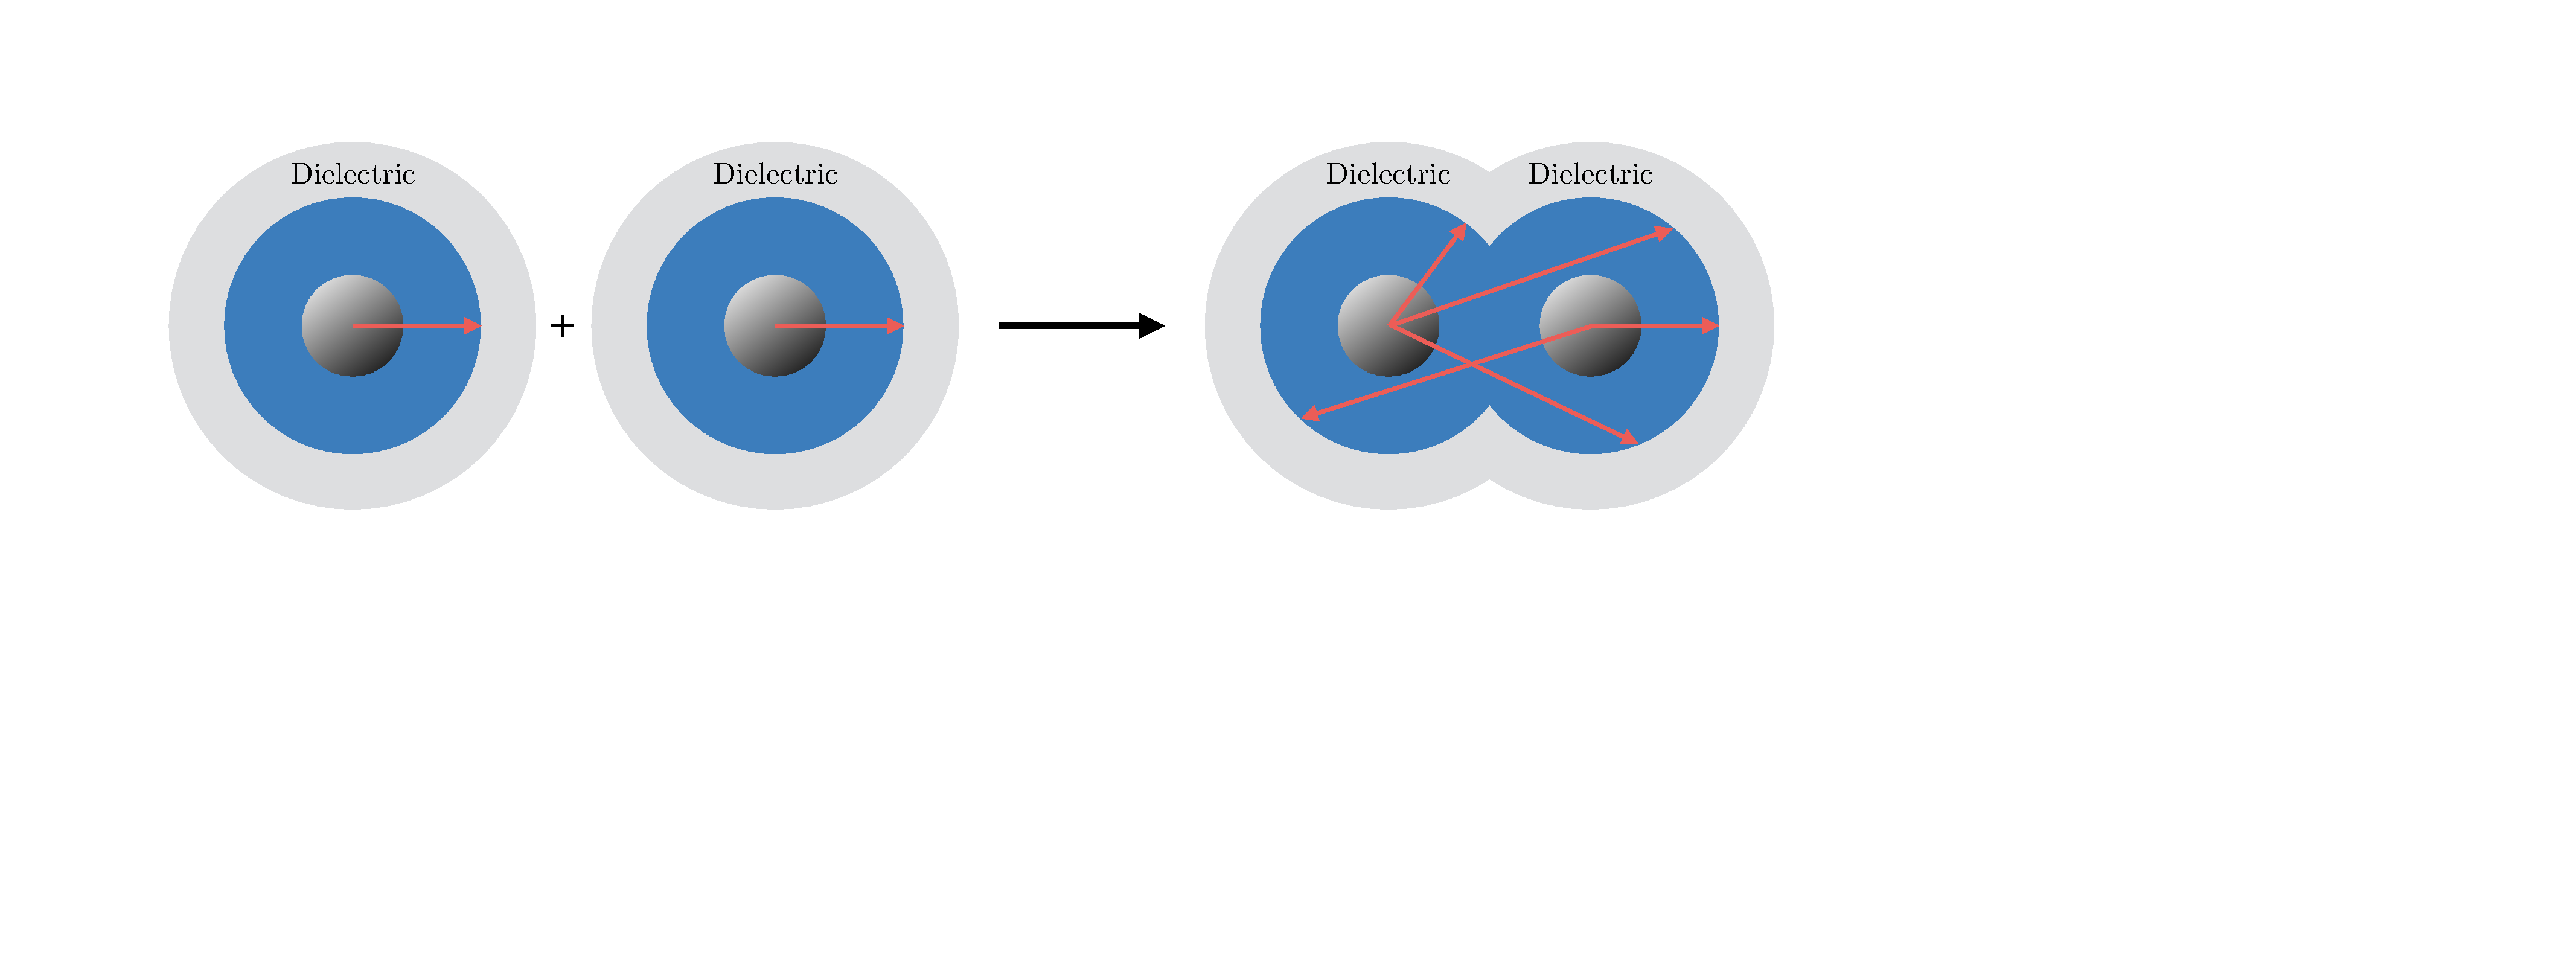
\includegraphics[scale=0.33]{figures/pdf/bornradius.pdf}
\caption{The pairwise nature of the Born radius.}
\label{bornrad}
\end{figure}
\vspace*{0.2cm}

The exponential function in \cref{genborn} is exploited to force $G_{\textrm{pol}}$ to approximate the dielectric part of Coulomb's law as atoms $i$ and $j$ move beyond the contact distance of their Born radii. It should be noted that solving \cref{genborn} for $G_{\textrm{pol}}$ is not trivial, owing to the pairwise nature of $\alpha_{ij}$; computing $\alpha_{ij}$ itself requires a numerical finite-difference method, which, while yielding well-defined Born radii, becomes prohibitively time-consuming as the systems under investigation become increasingly complex.

In the 1997 revision to GB/SA, \cite{qiu} the approach to calculating the Born radii was made fully analytical, circumventing the need to employ a numerical method to compute the electrostatic polarization term. This was accomplished by the definition of a new term, $G'_{\textrm{pol},i}$, \cref{gpoli}.

\begin{equation}
\label{gpoli}
G'_{\textrm{pol,}i} = \frac{-166.0}{R_{\textrm{vdW,}i}+\phi+P_1}+\sum^{\textrm{1,2}} \frac{P_2 V_j}{r_{ij}^{4}} + \sum^{\textrm{1,3}} \frac{P_3 V_j}{r_{ij}^{4}} + \sum^{\textrm{1,4,NB}} \frac{P_4 V_j \textrm{CCF}}{r_{ij}^{4}}
\end{equation}
\vspace*{-0.1cm}

\begin{figure}[b]
\centering
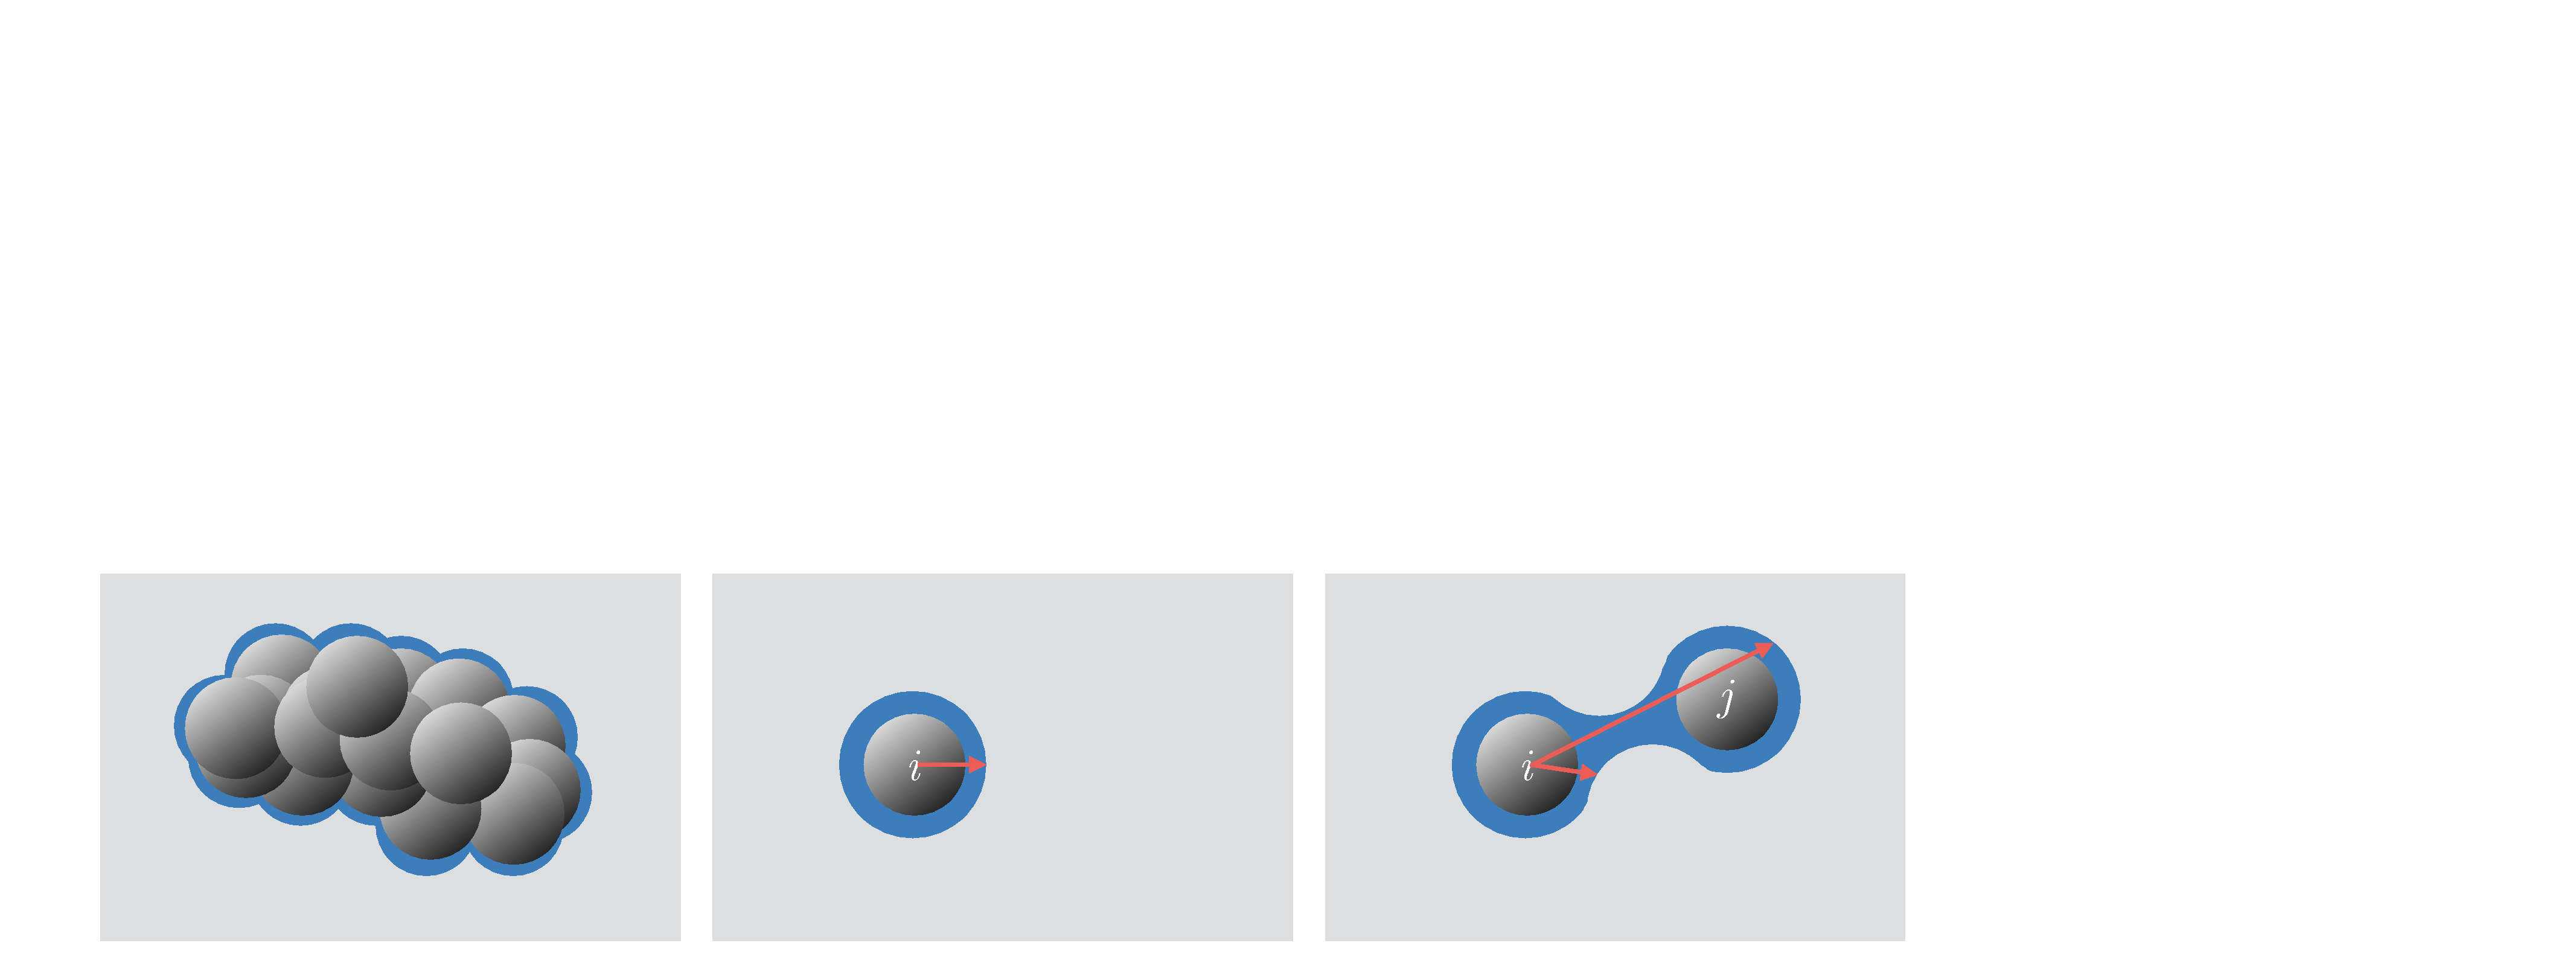
\includegraphics[scale=0.3]{figures/pdf/gpoli.pdf}\\
(a) \hspace*{4.4cm} (b) \hspace*{4.4cm} (c)
\caption{Born radii are calculated using the analytical approximation to $G_{\textrm{pol}}$.}
\label{figpoli}
\end{figure}

Thus, in \cref{gpoli}, the partial electrostatic contribution of atom $i$ is taken as the sum of self, 1,2, 1,3, 1,4, and 1,$>$4 terms relating to every other atom $j$. $P_{1}$--$P_{4}$ are optimized scaling factors for each respective interaction type, and CCF is a close-contact function for 1,4 and 1,$>$4 interactions. The dielectric offset, $\phi$, defines a gap between the edge of the van der Waals radius of atom $i$ and the beginning of the dielectric continuum, making the implicit solvent behave more like an explicit solvent. $V_{j}$ is the volume occupied by atom $j$, and $r_{ij}$ is the distance between atoms $i$ and $j$. The concept is illustrated in \cref{figpoli}. Imagine a system of neutral atoms, as in (a), where $G_{\textrm{pol}} = 0$. If one were to remove all the atoms except for one, and a charge were placed on that single atom, $i$, the system in (b) would then possess some nonzero $G_{\textrm{pol}}$, $G'_{\textrm{pol},i}$. Using the Born equation (\cref{born}), one could then easily compute $\alpha_{i}$. If one were to add a second atom $j$ back into the system but keep $j$ uncharged, then $G_{\textrm{pol}}$ would change by $V_{j}/r^{4}$ due to displacement of the continuum by atom $j$. Finally, placing the charge back onto $j$, as in (c), would change $G_{\textrm{pol}}$ by $G'_{\textrm{pol},j}$. The procedure could be repeated for all other atom pairs until a final $G_{\textrm{pol}}$ is achieved. This approach in principle makes the simulation of large biomolecular systems with GB/SA solvation much more feasible and has been widely accepted as the standard, modern form of GB/SA theory. \cite{jorg2005, jorg2004}

% ==========================================================================================
% ==========================================================================================
% ==========================================================================================

\subsection{GB/SA solvation in protein simulations.}

There is great appeal in employing implicit solvents in simulations of large biomolecular systems, \cite{bashford} primarily due to the simplification they can afford over systems modeled in explicit solvent. In the last 10 years, GB/SA has been widely used in the context of molecular dynamics simulations, including studies of RNA hairpin unfolding,\cite{sorin1} nucleic acid conformational dynamics,\cite{sorin2} and determination of free-energy surfaces of \textbeta-hairpin and \textalpha-helical peptides by replica-exchange molecular dynamics.\cite{felts} There is also precedent for the use of GB/SA in Metropolis\cite{metropolis} Monte Carlo simulations of biomolecular systems. For instance, flexible docking\cite{taylor} and concerted rotation with angles\cite{ulmschneider1, ulmschneider2} algorithms take advantage of GB/SA solvation.

Unfortunately, the number of reported studies using GB/SA in Monte Carlo simulations of proteins pales in comparison to the number of reported studies using GB/SA in molecular dynamics simulations of proteins, and few have exploited GB/SA in rigorous calculations of binding affinities. \cite{simonson, henchman, gallicchio, zhang} To understand this somewhat surprising finding, one must consider the impact of GB/SA theory on the methodological requirements of Monte Carlo vs.\ molecular dynamics simulations. Indeed, despite the simplification afforded by switching from an explicit to an implicit solvent model, simulations of large systems in implicit solvent can become similarly as computationally demanding as those in explicit solvent; whereas the computational demand and slow rate of convergence of modeling a system in explicit solvent arises from the large number of solvent molecules, high computational demand of modeling a system with GB/SA arises from the pairwise nature of the Born energy. For example, in a theoretical three-atom system consisting of atoms $i$, $j$, and $k$, the Born energy for atom pair $ij$ will change if the position of atom $k$ changes during a Monte Carlo move, because the Born radii of atoms $i$ and $j$ are both dependent on the position of atom $k$. Thus, in the context of a Monte Carlo simulation, one quickly finds that all atom-pair energies in a given system must be recalculated after every move, even if the position of most atoms in the system did not change. Accordingly, the sheer number of energy calculations that must be performed in a large system is staggering. Furthermore, a Monte Carlo simulation requires significantly more moves than a molecular dynamics simulation requires time steps; it is therefore not surprising that molecular dynamics simulations in GB/SA exhibit only a 4--5-fold increase in computation time relative to the gas phase,\cite{michel3} whereas we find that Monte Carlo simulations in GB/SA exhibit a 15--20-fold increase. In this light, the Monte Carlo method may quickly lose its appeal to those attempting to simulate large biomolecular systems with GB/SA. Nevertheless, the many powerful algorithms only available within a Monte Carlo manifold make it an indispensable tool for studying such systems.

Several modifications to the GB/SA model have been proposed in the literature.\cite{guvench, michel4, gelb, felts1} Rather than focusing on the form of $G_{\textrm{pol}}$, these approaches have developed procedures to determine which energies need to be recalculated after every move and which ones do not. For instance, the ``frozen atom'' approximation of Still and co-workers\cite{guvench} approximates the effects of atoms distant from the site of interest by freezing their coordinates throughout the duration of the simulation. Pairwise terms involving these frozen atoms therefore need to be calculated only once, and the derivatives thereof need not be calculated at all. In addition, a buffer region is defined, containing frozen atoms that are close enough to the site of interest to experience energetically significant changes to their Born radii as a result of the moving atoms. It quickly becomes apparent that given a setup such as this, different series of calculations can be performed for each atom pair based upon whether the pair is defined as frozen--frozen, moving--moving, buffer--frozen, or buffer--moving. This method was benchmarked using trial systems of camphor bound to cytochrome P450 and benzamidine bound to \textbeta-trypsin. Depending upon the system and the cutoff distance that was chosen, speed increases of approximately 1.5--10.6-fold were achieved.

A different approach was taken by Michel and co-workers\cite{michel4} in 2006, in which they used the pairwise descreening approximation (PDA)\cite{hawkins} for their description of the Born radii and structured their GB/SA implementation in such a way that the energy of an atom pair is only recalculated if the Born radius of either atom changes by more than a specified threshold after a Monte Carlo move. They determined the optimized threshold to be 0.005 \AA, yielding results within less than 0.1\% error of a fully rigorous calculation over the course of 5,000 moves. With this modification, a 3-fold speed increase was attained, and even with a threshold as low as 0.001 \AA, a 2.5-fold speed increase was attained. In addition, when the simplified sampling potential proposed by Gelb\cite{gelb} in 2003 was implemented alongside, the approximations afforded a 7--8-fold speed increase over a fully rigorous Monte Carlo GB/SA calculation.

% ==========================================================================================
% ==========================================================================================
% ==========================================================================================

\subsection{Monte Carlo free-energy perturbation.}

Free-energy perturbation (FEP) theory is a powerful method for calculating free-energy differences ($\Delta G$) of two different chemical states, \textbf{A} and \textbf{B}. Based on statistical mechanics and the Zwanzig equation,\cite{zwanzig} \cref{eqzwanzig}, it is used in both the molecular dynamics and Monte Carlo manifolds.
\vspace*{0.01cm}

\vspace*{-0.4cm}
\begin{equation}
\label{eqzwanzig}
\Delta G(\textrm{\textbf{A}} \longrightarrow \textrm{\textbf{B}}) = G_\textrm{\textbf{B}} - G_\textrm{\textbf{A}} = -k_{\textnormal{B}} T \ln \left\langle \textrm{exp} \left(- \frac{E_\textrm{\textbf{B}} - E_\textrm{\textbf{A}}}{k_{\textnormal{B}} T} \right) \right\rangle_\textrm{\textbf{A}}
\end{equation}
\vspace*{-0.5cm}

The difference in free energy between states \textbf{A} and \textbf{B} is calculated as an ensemble average of a simulation for state \textbf{A}. In practice, a Monte Carlo simulation is run for state \textbf{A} to determine $E_{\textrm{\textbf{A}}}$, and each time a new configuration is accepted, the energy $E_{\textrm{\textbf{B}}}$ is calculated for state \textbf{B} as well. For states that differ significantly, a scaling parameter $\lambda$ is used to divide the simulation into a series of small windows, allowing the system to be perturbed smoothly over several simulations from $\lambda = 0$ at state \textbf{A} to $\lambda = 1$ at state \textbf{B}. Simulations can also be run in reverse, from $\lambda = 1$ at state \textbf{B} to $\lambda = 0$ at state \textbf{A}, and hysteresis between the forward and backward simulations can be minimized by employing various techniques; using the smallest possible increments of $\lambda$ ensures smooth convergence and minimizes hysteresis. Typically, a doublewide sampling method is used, where an accepted configuration is perturbed to both $-\Delta\lambda$ and $+\Delta\lambda$ at once. Other sampling methods have been proposed, including overlap and double-ended variations.\cite{thomas} States \textbf{A} and \textbf{B} can differ in any number of ways, making FEP a very versatile computational tool. For instance, bond lengths or nonbonded interatomic distances can be perturbed from state \textbf{A} to \textbf{B}, yielding a potential energy-surface map along one or more sets of reaction coordinates. Alternately, atom types can be perturbed, simulating a theoretical mutation of molecule \textbf{A} into molecule \textbf{B}. The latter is particularly useful in determining relative free energies of hydration or relative free energies of binding. When doing so, the appropriate thermodynamic cycle is considered and two FEP calculations are performed independently. Examples are shown in \cref{thermocycle}.

\vspace*{0.2cm}
\begin{figure}[htbp]
\centering
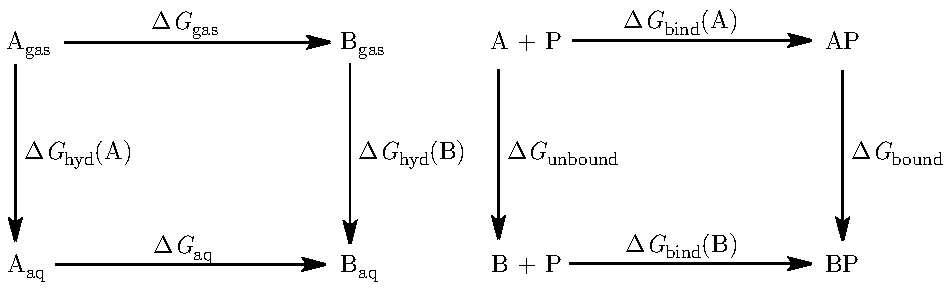
\includegraphics[scale=0.99]{figures/pdf/thermocycle.pdf}
\caption{Thermodynamic cycles for FEP-based determination of free energies of hydration (left) and binding (right).}
\label{thermocycle}
\end{figure}
\vspace*{0.2cm}

In \cref{thermocycle}, the thermodynamic cycle on the left represents a FEP simulation for calculating the relative free energy of hydration, $\Delta\Delta G_{\textrm{hyd}}$, between two molecules \textbf{A} and \textbf{B}. This quantity is determined in \cref{ddghyd} by perturbing molecule \textbf{A} into molecule \textbf{B} in both the gas phase and in aqueous solution, affording values for $\Delta G_{\textrm{gas}}(\textrm{\textbf{A}} \longrightarrow \textrm{\textbf{B}})$ and $\Delta G_{\textrm{aq}}(\textrm{\textbf{A}} \longrightarrow \textrm{\textbf{B}})$, respectively. \vspace*{-0.4cm}

\vspace*{-0.4cm}
\begin{equation}
\label{ddghyd}
\Delta G_{\textrm{aq}}(\textrm{\textbf{A}} \longrightarrow \textrm{\textbf{B}}) - \Delta G_{\textrm{gas}}(\textrm{\textbf{A}} \longrightarrow \textrm{\textbf{B}}) = \Delta G_{\textrm{hyd}}(\textrm{\textbf{B}}) - \Delta G_{\textrm{hyd}}(\textrm{\textbf{A}}) = \Delta\Delta G_{\textrm{hyd}}
\end{equation}
\vspace*{-0.8cm}

Similarly in \cref{thermocycle}, the thermodynamic cycle on the right depicts a FEP simulation for calculating relative free energies of binding, $\Delta\Delta G_{\textrm{bind}}$, between two ligands \textbf{A} and \textbf{B} to a protein \textbf{P}. This quantity is determined in \cref{ddgbind} by perturbing ligand \textbf{A} into ligand \textbf{B} in both the unbound and bound states, affording values for $\Delta G_{\textrm{unbound}}(\textrm{\textbf{A}} \longrightarrow \textrm{\textbf{B}})$ and $\Delta G_{\textrm{bound}}(\textrm{\textbf{AP}} \longrightarrow \textrm{\textbf{BP}})$, respectively. 

\vspace*{-0.8cm}
\begin{equation}
\label{ddgbind}
\Delta G_{\textrm{bound}}(\textrm{\textbf{AP}} \rightarrow \textrm{\textbf{BP}}) - \Delta G_{\textrm{unbound}}(\textrm{\textbf{A}} \rightarrow \textrm{\textbf{B}}) = \Delta G_{\textrm{bind}}(\textrm{\textbf{B}}) - \Delta G_{\textrm{bind}}(\textrm{\textbf{A}}) = \Delta\Delta G_{\textrm{bind}}
\end{equation}
\vspace*{-0.8cm}

Of course, for realistic free energies of binding, solvation (typically by water) must be accounted for in both the unbound and bound states.

The implications of this theory to those the field of computer-aided drug design are exciting, to say the least; for any molecule \textbf{A} whose biological activity is known or well predicted, any number of modifications can be made and the relative biological activity for the derivative \textbf{B} can be easily predicted. Results can be corroborated by biological assay and further structural or chemical refinements can be made as necessary. Application of this theory can allow investigators to screen large sets of potential drug candidates with relative ease or to optimize an already-promising lead, making it more potent or perhaps altering its binding mode to target mutations in the host.\cite{jorg2004sc}

% ==========================================================================================
% ==========================================================================================
% ==========================================================================================

\subsection{Investigative focus.}

The problem of correctly capturing the effects of solvation in applications of computer-aided drug design is not a trivial one, owing to large system size, structural complexity of solutes, mathematical obstacles, and stringent methodological requirements. Although continuum solvent models can aid in some of these aspects, they have historically been an incomplete solution to the problem; for example, the GB/SA solvation model is generally not amenable to FEP methods used in drug design, and specific details of implementation within a software package further complicate compatibility. Thus, we sought modification of the methodological approach to GB/SA calculations in the context of Monte Carlo free-energy perturbation. Our implementation is modeled after that of Michel, Taylor, and Essex.\cite{michel4} This approximation is based on the assumption that the impact of a moving atom on the Born radius of a distant atom is small, and therefore that a significant number of pairwise energy calculations can be omitted with little to no impact on the total energy change of the system after a Monte Carlo move. We sought to implement, test, and validate these modifications using real-world systems like those seen in our current drug-design projects, including benchmarking to document the performance of different subroutines and statistical analysis to fully understand the impact of our approximations.

% ==========================================================================================
% ==========================================================================================
% ==========================================================================================

\section{Experimental design and results.}

The scope of this work was three-fold. The first goal was to evaluate the existing implementation of GB/SA in terms of both performance and accuracy. The second goal was to modify the existing implementation of GB/SA to be compatible with existing FEP subroutines and to evaluate the performance and accuracy of both small and large FEP/GBSA simulations. Free energies of binding were to be compared to analogous ones in TIP4P explicit water. The third goal was to implement an approximated generalized Born potential, modeled after that of Michel, Taylor, and Essex.\cite{michel4} The effects of the approximation were to be evaluated in terms of speed, accuracy, and ability to scale, again comparing free energies of binding to those of analogous TIP4P simulations. In all cases, care was taken to adhere to the appropriate standards of system setup, end-user involvement, and consideration of available computational resources.

In the search for non-nucleoside inhibitors of HIV-1 reverse transcriptase, lead optimization of structures that were generated from similarity searches have lead to active compounds consisting of a 1,3,4-oxadiazole core linking a phenyl and an anilinyl ring.\cite{barreiro1, barreiro2} We chose as our test system a structure from an NNRTI series for HIV-RT, consisting of a parent ligand 5-benzyl-$N$-phenyl-1,3,4-oxadiazol-2-amine and ten of its monochloro analogs bound to HIV-1 RT. The protein scoop contained 2,728 atoms in 178 residues, and the parent ligand contained 30 atoms. The parent ligand \textbf{1} is shown in \cref{parent}. 

\begin{figure}
\centering
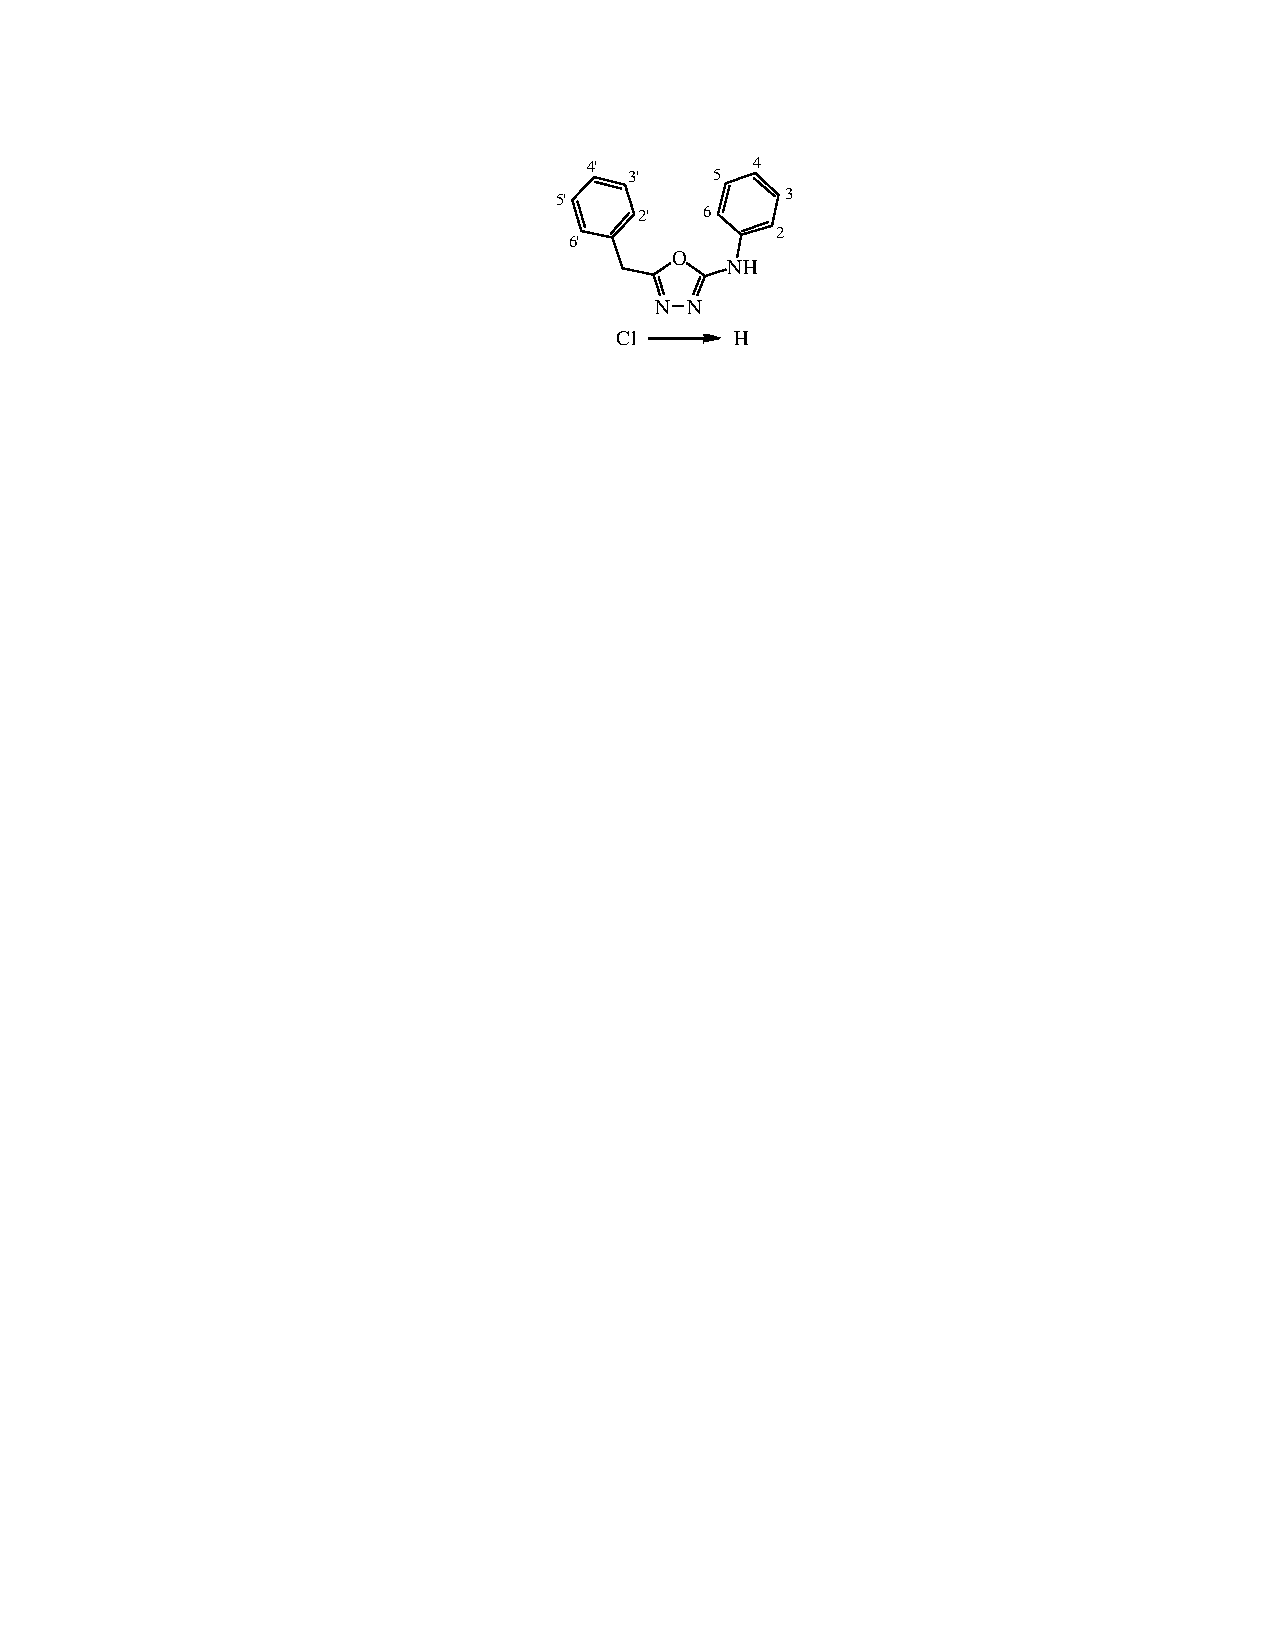
\includegraphics[scale=0.99]{figures/pdf/parent.pdf}
\caption{The parent ligand \textbf{1}, 5-benzyl-$N$-phenyl-1,3,4-oxadiazol-2-amine, in our test system. Monochloro substitution has been investigated at the ten positions indicated.}
\label{parent}
\end{figure}

Additional test cases used throughout this work consisted of two sets of small organic molecules involving perturbations commonly seen in FEP simulations of drug-like molecules, including a PhX $\longrightarrow$ PhY series, \cref{small,phxphy}. Unless otherwise noted, all calculations were performed using a modified version of \textit{MCPRO} \cite{jorgmcp} version 2.05 on Linux.

\begin{table}[p]
\centering
\caption{Test perturbations of small organic molecules.}
\begin{tabular}{rcl}
\toprule
PhCH$_3$  & $\longrightarrow$ &  PhOH \\
PhC(O)CH$_3$  & $\longrightarrow$ &  PhEt \\
Benzene  & $\longrightarrow$ &  Pyridine   \\
Cyclohexane  & $\longrightarrow$ &  THP \\
THP & $\longrightarrow$ & Dioxane   \\
Piperidine & $\longrightarrow$ &  THP    \\
AcOCH$_3$ & $\longrightarrow$ & AcOH    \\
AcOH & $\longrightarrow$ & Acetone   \\
AcNH$_2$ & $\longrightarrow$ & AcOH   \\
N(CH$_3$)$_3$ & $\longrightarrow$ & Acetone   \\ 
N(CH$_3$)$_3$ & $\longrightarrow$ & NH(CH$_3$)$_2$   \\ 
NH(CH$_3$)$_2$ & $\longrightarrow$ & CH$_3$NH$_2$   \\
iPrCl & $\longrightarrow$ & Propane   \\
Propane & $\longrightarrow$ & Ethane   \\
Propane & $\longrightarrow$ & $n$-PrBr   \\
\bottomrule
\end{tabular}
\label{small}
\end{table}

\begin{table}[p]
\centering
\caption{Test perturbations featuring the PhX $\longrightarrow$ PhY motif.}
\begin{tabular}{rcl}
\toprule
PhBr  & $\longrightarrow$ &  PhCl \\
PhCH$_3$         & $\longrightarrow$ & PhCF$_3$   \\
PhCl         & $\longrightarrow$ & PhF  \\
PhCl         & $\longrightarrow$ & Benzene   \\
PhF         & $\longrightarrow$ &  Benzene \\
PhCN       & $\longrightarrow$ &  PhF \\
PhC(O)CH$_3$  & $\longrightarrow$ & PhC(O)NH$_2$  \\
PhC(O)CH$_3$  & $\longrightarrow$ & PhNO$_2$  \\
PhEt         & $\longrightarrow$ & PhCH$_3$  \\
PhEt         & $\longrightarrow$ & PhOCH$_3$  \\
PhPr         & $\longrightarrow$ & BzOCH$_3$ \\
PhSH         & $\longrightarrow$ & PhOH  \\
iPrPh         & $\longrightarrow$ & PhEt  \\
PhCH$_3$         & $\longrightarrow$ & PhCl   \\
PhCH$_3$         & $\longrightarrow$ & Benzene  \\
PhCH$_3$         & $\longrightarrow$ & PhNH$_{2}$  \\
PhNO$_2$     & $\longrightarrow$ & PhOH  \\
PhNHCH$_3$       & $\longrightarrow$ & PhNH$_{2}$  \\ 
PhOH         & $\longrightarrow$ &  PhF \\
PhOH          & $\longrightarrow$ & PhOCH$_3$  \\
PhOCH$_3$        & $\longrightarrow$ & PhOH  \\
PhSCH$_3$         & $\longrightarrow$ & PhOCH$_3$  \\
\bottomrule
\end{tabular}
\label{phxphy}
\end{table} 

% ==========================================================================================
% ==========================================================================================
% ==========================================================================================

\subsection{Preliminary evaluation of GB/SA performance.}

To evaluate the performance and accuracy of the unmodified version of GB/SA in \textit{MCPRO}, standard Monte Carlo simulations were performed on our test system (\textbf{1}, \cref{parent}) bound and unbound, in the gas phase and with GB/SA, with \num{1.66e5} configurations of equilibration followed by \num{5.0e5} configurations of averaging for each of 14 windows of doublewide sampling. These values are scaled by 1/60 from those of a typical simulation in explicit water to account for the solute/solvent move ratio. Periodically, interactions of residues of similar charge were monitored; in our experience when using GB/SA in simulations of large proteins, the Coulombic forces between residues are often miscalculated if the GB/SA parameterization for the Born radii is not correct. For instance, two lysine residues might be brought together or even fused if the exaggeration is large enough. We envisioned that this could be a problem that would need to be addressed before proceeding with any further enhancements of the GB/SA model. Gratifyingly, our inspections revealed no such phenomena. Benchmark simulation times are given in \cref{prelim}. 

\begin{table}[htbp]
\centering
\caption{Preliminary Monte Carlo benchmarking results for our test system.}
\begin{tabular}{cccc}
\toprule
Conditions              & Simulation time (h) & $\Delta t_{\textrm{bound vs. unbound}}$ & $\Delta t_{\textrm{GB/SA vs.\ gas}}$ \\
\midrule
Unbound, gas phase      & 0.43                & --                                                     & --\\
Bound,   gas phase      & 4.51                & 10.5$x$                                                & --\\
Unbound, GB/SA          & 0.62                & --                                                     & 1.44$x$\\
Bound,   GB/SA          & 76                  & 123$x$                                                 & 16.8$x$\\
\bottomrule
\end{tabular}%
\label{prelim}%
\end{table}%

\cref{prelim} shows several pieces of data of which it was important to remain cognizant while proceeding. First, the gas-phase simulations took approximately 10.5 times longer to complete in the bound form than in the unbound form, giving a sense of the size of the bound system relative to the unbound. Not surprisingly, the efficiency of the GB/SA simulations deteriorated rapidly with increasing system size: the GB/SA calculations took 123 times longer to complete in the bound form in the unbound form. Perhaps more interesting is the comparison of gas-phase simulation times to GB/SA simulation times. These data indicate that for the unbound system (comprised of 30 atoms), GB/SA simulation times were roughly on par with those in the gas phase, costing a slowdown of only a few minutes. However, the simulation of the bound ligand \textbf{1} in GB/SA took nearly 17 times longer than it did in the gas phase, leaving ample room for improvement.

In the unmodified version of \textit{MCPRO}, single-point energy calculations and standard Monte Carlo simulations (both of which are nonperturbing techniques) were the only tools available with GB/SA solvation. Nevertheless, energies could still be calculated that were in some ways analogous to those acquired via Monte Carlo FEP in TIP4P explicit water. For example, relative free energies of solvation could be determined by using single-point GB/SA energy calculations for the initial and final states (\textbf{A} and \textbf{B}, respectively), \cref{eqsp}.

\vspace*{-0.3cm}
\begin{equation}
\label{eqsp}
\Delta G_{\textrm{sol}} \textrm{(SP/GBSA,\textbf{B})} - \Delta G_{\textrm{sol}} \textrm{(SP/GBSA,\textbf{A})} = \Delta\Delta G_{\textrm{sol}}\textrm{(SP/GBSA)}
\end{equation}

The value of $\Delta\Delta G_{\textrm{sol}}\textrm{(SP/GBSA)}$ is analogous to $\Delta\Delta G_{\textrm{sol}}\textrm{(TIP4P)}$, which could be computed using our standard MC/FEP protocol with TIP4P explicit water, \cref{eqtip}.

\begin{equation}
\label{eqtip}
\Delta G \textrm{(FEP/TIP4P)} - \Delta G \textrm{(FEP/Vacuum)} = \Delta\Delta G_{\textrm{sol}}\textrm{(TIP4P)}
\end{equation}
\vspace*{-0.8cm}


Although these two energies are arrived upon by very different algorithms (single-point energy calculations involve no sampling whatsoever), during the early stage of the investigation we were interested in whether or not the effect of the water sampling in MC/FEP could be captured in simple single-point energy calculations with GB/SA solvation. Thus, values of $\Delta\Delta G_{\textrm{sol}}\textrm{(SP/GBSA)}$ and $\Delta\Delta G_{\textrm{sol}}\textrm{(TIP4P)}$ were computed for the entire test set of 55 small- to mid-size organic molecules. For the MC/FEP calculations in TIP4P explicit water, \num{1.0e7} configurations of equilibration and \num{3.0e7} configurations of averaging were accumulated with solute moves attempted every 60 configurations. The doublewide sampling method was used over 14 windows. Calculations took between 7 and 55 times longer with TIP4P compared to those in the gas phase; CPU times for GB/SA single-point calculations were negligible. A correlation plot is shown in \cref{precorr}. 

\begin{figure}[b!]
\centering
% GNUPLOT: LaTeX picture with Postscript
\begingroup
  \makeatletter
  \providecommand\color[2][]{%
    \GenericError{(gnuplot) \space\space\space\@spaces}{%
      Package color not loaded in conjunction with
      terminal option `colourtext'%
    }{See the gnuplot documentation for explanation.%
    }{Either use 'blacktext' in gnuplot or load the package
      color.sty in LaTeX.}%
    \renewcommand\color[2][]{}%
  }%
  \providecommand\includegraphics[2][]{%
    \GenericError{(gnuplot) \space\space\space\@spaces}{%
      Package graphicx or graphics not loaded%
    }{See the gnuplot documentation for explanation.%
    }{The gnuplot epslatex terminal needs graphicx.sty or graphics.sty.}%
    \renewcommand\includegraphics[2][]{}%
  }%
  \providecommand\rotatebox[2]{#2}%
  \@ifundefined{ifGPcolor}{%
    \newif\ifGPcolor
    \GPcolortrue
  }{}%
  \@ifundefined{ifGPblacktext}{%
    \newif\ifGPblacktext
    \GPblacktextfalse
  }{}%
  % define a \g@addto@macro without @ in the name:
  \let\gplgaddtomacro\g@addto@macro
  % define empty templates for all commands taking text:
  \gdef\gplbacktext{}%
  \gdef\gplfronttext{}%
  \makeatother
  \ifGPblacktext
    % no textcolor at all
    \def\colorrgb#1{}%
    \def\colorgray#1{}%
  \else
    % gray or color?
    \ifGPcolor
      \def\colorrgb#1{\color[rgb]{#1}}%
      \def\colorgray#1{\color[gray]{#1}}%
      \expandafter\def\csname LTw\endcsname{\color{white}}%
      \expandafter\def\csname LTb\endcsname{\color{black}}%
      \expandafter\def\csname LTa\endcsname{\color{black}}%
      \expandafter\def\csname LT0\endcsname{\color[rgb]{1,0,0}}%
      \expandafter\def\csname LT1\endcsname{\color[rgb]{0,1,0}}%
      \expandafter\def\csname LT2\endcsname{\color[rgb]{0,0,1}}%
      \expandafter\def\csname LT3\endcsname{\color[rgb]{1,0,1}}%
      \expandafter\def\csname LT4\endcsname{\color[rgb]{0,1,1}}%
      \expandafter\def\csname LT5\endcsname{\color[rgb]{1,1,0}}%
      \expandafter\def\csname LT6\endcsname{\color[rgb]{0,0,0}}%
      \expandafter\def\csname LT7\endcsname{\color[rgb]{1,0.3,0}}%
      \expandafter\def\csname LT8\endcsname{\color[rgb]{0.5,0.5,0.5}}%
    \else
      % gray
      \def\colorrgb#1{\color{black}}%
      \def\colorgray#1{\color[gray]{#1}}%
      \expandafter\def\csname LTw\endcsname{\color{white}}%
      \expandafter\def\csname LTb\endcsname{\color{black}}%
      \expandafter\def\csname LTa\endcsname{\color{black}}%
      \expandafter\def\csname LT0\endcsname{\color{black}}%
      \expandafter\def\csname LT1\endcsname{\color{black}}%
      \expandafter\def\csname LT2\endcsname{\color{black}}%
      \expandafter\def\csname LT3\endcsname{\color{black}}%
      \expandafter\def\csname LT4\endcsname{\color{black}}%
      \expandafter\def\csname LT5\endcsname{\color{black}}%
      \expandafter\def\csname LT6\endcsname{\color{black}}%
      \expandafter\def\csname LT7\endcsname{\color{black}}%
      \expandafter\def\csname LT8\endcsname{\color{black}}%
    \fi
  \fi
  \setlength{\unitlength}{0.0500bp}%
  \begin{picture}(7200.00,5040.00)%
    \gplgaddtomacro\gplbacktext{%
      \csname LTb\endcsname%
      \put(682,880){\makebox(0,0)[r]{\strut{}-8}}%
      \csname LTb\endcsname%
      \put(682,1436){\makebox(0,0)[r]{\strut{}-6}}%
      \csname LTb\endcsname%
      \put(682,1993){\makebox(0,0)[r]{\strut{}-4}}%
      \csname LTb\endcsname%
      \put(682,2549){\makebox(0,0)[r]{\strut{}-2}}%
      \csname LTb\endcsname%
      \put(682,3106){\makebox(0,0)[r]{\strut{} 0}}%
      \csname LTb\endcsname%
      \put(682,3662){\makebox(0,0)[r]{\strut{} 2}}%
      \csname LTb\endcsname%
      \put(682,4219){\makebox(0,0)[r]{\strut{} 4}}%
      \csname LTb\endcsname%
      \put(682,4775){\makebox(0,0)[r]{\strut{} 6}}%
      \csname LTb\endcsname%
      \put(814,660){\makebox(0,0){\strut{}-12}}%
      \csname LTb\endcsname%
      \put(1479,660){\makebox(0,0){\strut{}-10}}%
      \csname LTb\endcsname%
      \put(2145,660){\makebox(0,0){\strut{}-8}}%
      \csname LTb\endcsname%
      \put(2810,660){\makebox(0,0){\strut{}-6}}%
      \csname LTb\endcsname%
      \put(3476,660){\makebox(0,0){\strut{}-4}}%
      \csname LTb\endcsname%
      \put(4141,660){\makebox(0,0){\strut{}-2}}%
      \csname LTb\endcsname%
      \put(4807,660){\makebox(0,0){\strut{} 0}}%
      \csname LTb\endcsname%
      \put(5472,660){\makebox(0,0){\strut{} 2}}%
      \csname LTb\endcsname%
      \put(6138,660){\makebox(0,0){\strut{} 4}}%
      \csname LTb\endcsname%
      \put(6803,660){\makebox(0,0){\strut{} 6}}%
      \csname LTb\endcsname%
      \put(250,2827){\rotatebox{-270}{\makebox(0,0){\strut{}$\Delta\Delta G_\textrm{sol}$(SP/GBSA)}}}%
      \put(3808,330){\makebox(0,0){\strut{}$\Delta\Delta G_\textrm{sol}$(FEP/TIP4P)}}%
    }%
    \gplgaddtomacro\gplfronttext{%
    }%
    \gplbacktext
    \put(0,0){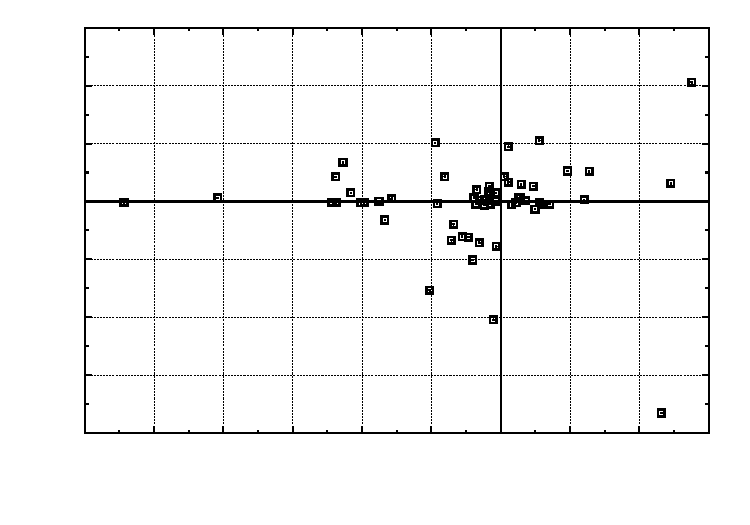
\includegraphics{figures/precorr/precorr}}%
    \gplfronttext
  \end{picture}%
\endgroup

\caption{Relative free energies of solvation determined by SP with GB/SA and MC/FEP with TIP4P. Values are in kcal/mol. No correlation is observed ($r^{2} = 0.0002$).}
\label{precorr}
\end{figure}

As is clear, there is essentially no correlation ($r^{2} = 0.0002$) between the relative free energies of solvation computed via MC/FEP in TIP4P explicit water and those determined from single-point calculations with GB/SA, and similar results could be expected for relative free energies of binding. Therefore, as was anticipated, the tools currently available with GB/SA solvation were insufficient for applications in drug design and as such there was clear motivation to pursue modifications allowing the use of GB/SA in the context Monte Carlo free-energy perturbation.

% ==========================================================================================
% ==========================================================================================
% ==========================================================================================

\subsection{Program structure and technical challenges.}

The unmodified version of GB/SA as implemented in \textit{MCPRO} was not compatible with MC/FEP simulations in part because it assumed a static approach to atomic properties, whereas in FEP, properties such as van der Waals radii, atomic volumes (minus any overlap with neighboring atoms), and Coulombic charges must be dynamically adjusted and scaled as perturbations are made. For example, in the unmodified GB/SA implementation, the charges for saturated alkanes were dealt with in a united-atom fashion, such that the charges of the alkane hydrogens were moved onto the attached alkane carbon. Thus, for methane, four formal charges of $+1.09$ corresponding to the four hydrogens were added onto the formal $-4.36$ charge on carbon, making all the atoms as a group Coulombically neutral. Although this type of simplification is often desirable, in a perturbation it can be logistically problematic. Take for instance the perturbation from methane to chloromethane, where a hydrogen atom is perturbed to a chlorine atom. In a united-atom approach with FEP, the charge on the perturbed hydrogen atom would need to be identified and smoothly moved off of the carbon, so that the charge would be fully condensed at the beginning of the perturbation but would be fully expanded, with the appropriate new charge and volume for chlorine, at the end of the perturbation. Switching from a united-atom approach to an all-atom approach would circumvent complications such at this, except that specific GB/SA parameters were originally developed with the united-atom approach in mind. Furthermore, as originally implemented, contribution of 1,2 and 1,3 interactions to $G'_{\textrm{pol,}i}$ in \cref{gpoli} were counted for certain types of 1,2 or 1,3 neighbors and were ignored for others. In a FEP simulation, however, these contributions might need to be counted for a given atom pair at one end of the perturbation but not at the other. Again in the case of perturbing methane to chloromethane, 1,2 interactions would be ignored entirely for methane, but would need to be counted only for the C--Cl atom pair in chloromethane.

Yet another component of FEP calculations that complicates integration with GB/SA is management of dummy atoms, which are special atom types whose properties are not felt by any other part of the system. Since an atom might require dummy characteristics at one end of the perturbation but not at the other, the properties of such atoms would also need to be dynamically adjusted and scaled as perturbations are made. When accommodating special cases like these, care must be taken to ensure that the energy of the system is not only consistent at any given point during the perturbation, but also that the change in energy of the system is smooth throughout the perturbation. Thus, several novel modifications were made to the GB/SA module in \textit{MCPRO} with the goal of making GB/SA calculations fully compatible with FEP simulations. Specific details follow.

A new subroutine, {\tt GETSIG}, is called at the initialization of each window in order to identify atoms whose initial and/or final states require special treatment for the determination of their van der Waals radii when FEP is being performed. Prior GB/SA code had no knowledge of initial and final states, a concept necessitated by many aspects of FEP calculations. In the original implementation of GB/SA in \textit{MCPRO}, atoms were assigned a van der Waals radius in one of two ways: either implicitly, based on their Lennard--Jones parameters $\varepsilon$ and $\sigma$ as given by \cref{eqlj}, or explicitly, based on the identity of the atom. For instance, the van der Waals radius of a benzene carbon is implicitly calculated to be 1.775 \AA{} based on its Lennard--Jones parameters, whereas the van der Waals radius for a hydrogen on a heteroatom is explicitly assigned to 1.15 \AA{} and the van der Waals radius for covalently bonded fluorine is explicitly assigned to 2.0 \AA. The implicitly based assignments are fully compatible with FEP, since the Lennard--Jones parameters are received by the GB/SA module after having been scaled appropriately by the FEP code base in \textit{MCPRO}\@. However, the explicit assignments are inherently incompatible with FEP since the identity of any given atom can change during an FEP run. Therefore, the {\tt GETSIG} subroutine acts as a decision-making ``switch'' to decide where and how van der Waals radii are assigned. If an FEP simulation with GB/SA solvation is requested, the {\tt GETSIG} subroutine checks initial and final atom types and explicitly assigns van der Waals radii to the appropriate atom types. Dummy atoms are treated explicitly at this point and are assigned a van der Waals radius of 1.15 \AA. If an atom requires an explicitly assigned van der Waals radius at one end of the perturbation and an implicitly calculated van der Waals radius at the other end, then special action is required: the Lennard--Jones parameters are determined for the atom type whose van der Waals radius would be implicitly calculated, and the van der Waals radius is then calculated for the appropriate state and stored as an explicitly assigned value. At the end of the {\tt GETSIG} subroutine, all initial and final van der Waals radii are passed to the {\tt GBSASETUP} subroutine, where scaled radii are calculated for the reference, first and second perturbed states, given by \cref{rvdwif}.

\vspace*{-.3cm}
\begin{equation}
\label{eqlj}
R_{ \textrm{vdW}} = \frac{1}{2} \left( \frac{\sqrt{4 \varepsilon \sigma^{12}}}{\sqrt{4 \varepsilon \sigma^{6}}} \right)^{1/3}
\end{equation}
\vspace*{-.5cm}

\vspace*{-0.7cm}
\begin{equation}
\label{rvdwif}
R_{ \textrm{vdW}} = \lambda R_{ \textrm{vdW}}(\textrm{Final}) + (1 - \lambda) R_{ \textrm{vdW}}(\textrm{Initial})
\end{equation}

Atoms whose van der Waals radii require no explicit assignment need no further treatment; the van der Waals radii for their reference, first and second perturbed states are calculated based solely on their pre-scaled Lennard--Jones parameters for the entirety of the simulation.

The {\tt GBSASETUP} subroutine in the GB/SA module is called immediately after the {\tt GETSIG} subroutine and is responsible for computing the first three terms of $G'_{\textrm{pol,}i}$ in \cref{gpoli}. This series of calculations required several significant modifications, the first of which was to include in FEP simulations the proper treatment of the united-atom approach to Coulombic charge on saturated alkyl groups. To this end, there are two scenarios: the first, where charges must be condensed at the beginning of the simulation but not at the end, and the second, where charges must be condensed at the end of the simulation but not at the beginning. Accounting for this is trivially accomplished by using the same scaling factor $\lambda$ used in the calculation of van der Waals radii.

Two examples can be used to illustrate the first scenario. First, in a perturbation from methane to chloromethane, the charge on the hydrogen that is perturbed to chlorine must be condensed in the case of methane but not in the case of chloromethane. Second, in a perturbation from methane to ammonia, the charge on all of the hydrogens must be condensed in the case of methane but not in the case of ammonia. Whereas the factors affecting charge condensation in the first example are determined by the identity of the hydrogen (atom $i$), in the second example they are determined by the identity of the carbon/nitrogen (atom $j$). In such events, scaling by $\lambda$ is performed as given in eqs \ref{qborn1} and \ref{qborn2}. Equations also apply for the first and second perturbed states.

\vspace*{-0.4cm}
\begin{equation}
\label{qborn1}
q_{\textrm{Born}}(i) = q_{\textrm{Born}}(i) + (1 - \lambda) q_{\textrm{Born}}(j)
\end{equation}
\vspace*{-1.7cm}

\begin{equation}
\label{qborn2}
q_{\textrm{Born}}(j) = \lambda q_{\textrm{Born}}(j)
\end{equation}
\vspace*{-0.7cm}

Thus, when the neighbor atom $j$ exhibits 100\% hydrogen-like characteristics (i.e., $\lambda = 0$), 100\% of $q_{\textrm{Born}}(j)$ is added onto $q_{\textrm{Born}}(i)$ and 0\% of $q_{\textrm{Born}}(j)$ is retained. Similarly, when the neighbor exhibits 50\% hydrogen-like characteristics (i.e., $\lambda = 0.5$), 50\% of $q_{\textrm{Born}}(j)$ is added onto $q_{\textrm{Born}}(i)$, and 50\% of $q_{\textrm{Born}}(j)$ is retained, and when the neighbor exhibits 0\% hydrogen-like characteristics (i.e., $\lambda = 1.0$), 0\% of $q_{\textrm{Born}}(j)$ is added onto $q_{\textrm{Born}}(i)$, and 100\% of $q_{\textrm{Born}}(j)$ is retained.

For the second scenario, two possible examples also exist, which are essentially the reverse of the examples given in the first scenario. One could envision perturbation from chloromethane to methane, where charge condensation is not required for the chlorine atom at the beginning of the simulation but is required for the hydrogen atom to which the chlorine atom is perturbed at the end of the simulation. Additionally, one could envision perturbation from ammonia to methane, where charge condensation is not required for the hydrogen atoms at the beginning of the simulation but is required for the hydrogen atoms at the end of the simulation, since the identity of the nitrogen is perturbed from nitrogen to carbon. Scaling by $\lambda$ is performed as given by eqs \ref{qborn3} and \ref{qborn4}. Equations also apply for the first and second perturbed states.

\vspace*{-.4cm}
\begin{equation}
\label{qborn3}
q_{\textrm{Born}}(i) = q_{\textrm{Born}}(i) + \lambda q_{\textrm{Born}}(j)
\end{equation}
\vspace*{-1.6cm}

\begin{equation}
\label{qborn4}
q_{\textrm{Born}}(j) = (1 - \lambda) q_{\textrm{Born}}(j)
\end{equation}
\vspace*{-0.7cm}

Thus, when the neighbor exhibits 100\% hydrogen-like characteristics (i.e., $\lambda$ = 0), 0\% of $q_{\textrm{Born}}(j)$ is added onto $q_{\textrm{Born}}(i)$ and 100\% of $q_{\textrm{Born}}(j)$ is retained. Similarly, when the neighbor exhibits 50\% hydrogen-like characteristics (i.e., $\lambda$ = 0.5), 50\% of $q_{\textrm{Born}}(j)$ is added onto $q_{\textrm{Born}}(i)$, and 50\% of $q_{\textrm{Born}}(j)$ is retained, and when the neighbor exhibits 0\% hydrogen-like characteristics (i.e., $\lambda$ = 1.0), 100\% of $q_{\textrm{Born}}(j)$ is added onto $q_{\textrm{Born}}(i)$, and 0\% of $q_{\textrm{Born}}(j)$ is retained.

Another modification requiring similar attention to detail was the Coulombic charge correction to N--O compounds. As standard procedure, in the event of an N--O group 24\% of the oxygen's charge is added to the nitrogen and removed from the oxygen. Since the decision to make such a correction is dependent on nonstatic atom types, in the unmodified implementation of GB/SA in \textit{MCPRO} this correction was not compatible with FEP. Simple decision-making statements were added to identify N--O pairs that are perturbed to non-N--O pairs, and in such events, the percent of the correction that is made is scaled from 100\% at the beginning of the simulation to 0\% at the end of the simulation. Similarly, for non-N--O pairs that are perturbed to N--O pairs, the percent of the correction that is made is scaled from 0\% at the beginning of the simulation to 100\% at the end of the simulation. In modifying the GB/SA module to accommodate FEP in calculating atomic volumes, a significant challenge was encountered in correctly calculating volume overlap of adjacent atoms. Generally, the atomic volume for an atom $i$ is calculated as the volume of a sphere with radius $R_{ \textrm{vdW}}$, minus the sum of any volume overlap from 1,2 neighboring atoms $j$. However, for certain atom-type pairs (such as C--F in fluoromethane), this method of calculating overlap of two atoms $i$ and $j$ can yield negative overlap, \cref{olap}.\vspace*{-0.6cm}

\vspace*{-.4cm}
\begin{equation}
\label{olap}
\textrm{overlap}(i) = (\pi/3)(R_{ \textrm{vdW}}(i)(1+ \textrm{ratio}))^{2}\cdot(3R_{ \textrm{vdW}}(i) - R_{ \textrm{vdW}}(i)(1+ \textrm{ratio}))
\end{equation}
\vspace*{-1.7cm}

\begin{equation*}
\textrm{where ratio} = \frac{R^{2}_{ \textrm{vdW}}(j) - R^{2}_{ \textrm{vdW}}(i) - r^{2}_{0}}{2R_{ \textrm{vdW}}(i) \cdot r_{0}}
\end{equation*}
\vspace*{-0.4cm}

For FEP calculations where both bond lengths and van der Waals radii change, the problem is exacerbated and volumes can become even more negative. Moreover, overlap of dummy atoms becomes problematic since they are given nonzero van der Waals radii. This was remedied through several adjustments: first, a maximum value of 1.000 was set for the ratio term, effectively restricting the perturbation so that an atom cannot be overlapped by a volume greater than its own. Second, the overlap for neighboring atoms that are perturbed to or from dummy atoms is scaled by $\lambda$ such that 100\% overlap is counted when the atom is not a dummy and 0\% overlap is counted when the atom is a dummy. Lastly, a minimum volume is set to 1.000 \AA$^{3}$ after overlap for all atoms to prevent division by zero for atoms that are completely overlapped by neighbors.

Yet another aspect of the GB/SA implementation that becomes problematic in FEP calculations is the fact that 1,2 and 1,3 contributions to the electrostatic term are not counted for alkane C--H atom pairs; in the event of an FEP simulation where an alkane C--H atom pair is perturbed in some way, the 1,2 and/or 1,3 contribution must be turned on or off. The initial appearance of the electrostatic term, $G'_{ \textrm{pol},i}$, is defined in \cref{buildpoli1} where $P_{1} = 0.073$. This also applies for the first and second perturbed states. Note that dummy atoms, which were assigned a minimum $R_{ \textrm{vdW}}$ of 1.15 \AA, acquire a nonzero  $G'_{ \textrm{pol},i}$ at this stage, which is incorrect and will be addressed later in the calculation of Born energies.

\vspace*{-0.4cm}
\begin{equation}
\label{buildpoli1}
G'_{ \textrm{pol},i} = \frac{-166.0}{0.09\cdot R_{ \textrm{vdW}}\cdot P_{1}}
\end{equation}
\vspace*{-0.5cm}


Several decision-making steps are then taken in order to correctly account for 1,2 and 1,3 interactions for certain atom-type pairs. Contribution of 1,2 interactions is ignored completely for hydrogen on CT/CY saturated carbons and for saturated carbons on hydrogen. Otherwise, full contribution of 1,2 interactions is given for the reference, first and second perturbed states by \cref{buildpoli2}, where $P_{2} = 0.921$.

\begin{equation}
\label{buildpoli2}
G'_{ \textrm{pol},i} = G'_{ \textrm{pol},i} + (P_{2}V_{j})(1/r^{4}_{0})
\end{equation}
\vspace*{-0.4cm}

In the event of FEP, contribution of 1,2 interactions is ignored completely for the following pair transformations, where both the initial and final states include pairs for which 1,2 electrostatic contribution must be ignored.

\vspace*{.4cm}
\begin{singlespace}
{\centering
\begin{tabular}{rcl}
C--H   & $\longrightarrow$ & C--DUM \\
C--H   & $\longrightarrow$ & DUM--C \\
H--C   & $\longrightarrow$ & C--DUM \\
H--C   & $\longrightarrow$ & DUM--C \\
C--DUM & $\longrightarrow$ & C--H \\
C--DUM & $\longrightarrow$ & H--C \\
DUM--C & $\longrightarrow$ & H--C \\
DUM--C & $\longrightarrow$ & C--H \\
N--DUM & $\longrightarrow$ & C--H/DUM \\
DUM--N & $\longrightarrow$ & H/DUM--C \\
\end{tabular}\\}
\end{singlespace}\vspace*{.7cm}

Several cases exist where 1,2 electrostatic contribution must be scaled on throughout the course of an FEP simulation. Such pair transformations include, but are not limited to, the following, where the initial state involves non-1,2-contributing pairs and the final state includes 1,2-contributing pairs.

\vspace*{.5cm}
\begin{singlespace}
{\centering
\begin{tabular}{rcl}
C--H/DUM & $\longrightarrow$ & C--C \\
H/DUM--C & $\longrightarrow$ & C--C \\
N--DUM   & $\longrightarrow$ & N--H \\
DUM--N   & $\longrightarrow$ & H--N \\
\end{tabular}\\}
\end{singlespace}\vspace*{.7cm}

Thus, 1,2 contribution for these pairs is scaled so that 0\% is added at $\lambda$ = 0 and 100\% is added at $\lambda$ = 1, for the reference, first and second perturbed states as in \cref{buildpoli3}.

\begin{equation}
\label{buildpoli3}
G'_{ \textrm{pol},i} = G'_{ \textrm{pol},i} + \lambda(P_{2}V_{j})(1/r^{4}_{0})
\end{equation}
\vspace*{-0.4cm}

Similarly, several cases exist where 1,2 electrostatic contribution must be scaled off throughout the course of an FEP simulation. Such pair transformations include, but are not limited to, the following, where the initial state involves 1,2-contributing pairs and the final state includes non-1,2-contributing pairs.

\vspace*{.4cm}
\begin{singlespace}
{\centering
\begin{tabular}{rcl}
C--C & $\longrightarrow$ & C--H/DUM \\ 
C--C & $\longrightarrow$ & H/DUM--C \\
N--H & $\longrightarrow$ & N--DUM \\
H--N & $\longrightarrow$ & DUM--N \\
\end{tabular}\\}
\end{singlespace}
\vspace*{.6cm}

Thus, 1,2 contribution by for these pairs is scaled so that 100\% is added at $\lambda$ = 0 and 0 is added at $\lambda$ = 1, for the reference, first and second perturbed states as in \cref{buildpoli4}.

\vspace*{-.4cm}
\begin{equation}
\label{buildpoli4}
G'_{ \textrm{pol},i} = G'_{ \textrm{pol},i} + (1 - \lambda)(P_{2}V_{j})(1/r^{4}_{0})
\end{equation}
\vspace*{-0.6cm}

Similar steps are taken for 1,3 electrostatic contribution. Again, 1,3 electrostatic contribution is ignored for hydrogen on CT/CY saturated carbons and for saturated carbons on hydrogen; it is included fully for other cases where no FEP has been requested, and is scaled by $\lambda$ for cases where 1,3 contribution must be turned on or off throughout the course of an FEP simulation. Such cases are identical to those for 1,2 contribution, and are given in eqs \ref{buildpoli5}--\ref{buildpoli7}, where $P_{3} = 6.211$. Equations apply for the first and second perturbed states as well. It should be noted that all {\tt GETSIG} and {\tt GBSASETUP} assignments and calculations up to this point are made once at the initialization of each window and are held constant throughout the remaining moves of that window; only the 1,4 and 1,$>$4 contributions to the energy are reevaluated after every move, since the 1,2 and 1,3 relationships (and thus the 1,2 and 1,3 electrostatic contributions) are unlikely to change within a given window.

\vspace*{-0.6cm}
\begin{equation}
\label{buildpoli5}
G'_{ \textrm{pol},i} = G'_{ \textrm{pol},i} + (P_{3}V_{k})(1/r^{4}_{0})
\end{equation}
\vspace*{-1.65cm}

\begin{equation}
\label{buildpoli6}
G'_{ \textrm{pol},i} = G'_{ \textrm{pol},i} + \lambda(P_{3}V_{k})(1/r^{4}_{0})
\end{equation}
\vspace*{-1.65cm}

\begin{equation}
\label{buildpoli7}
G'_{ \textrm{pol},i} = G'_{ \textrm{pol},i} + (1-\lambda)(P_{3}V_{k})(1/r^{4}_{0})
\end{equation}
\vspace*{-0.7cm}

From this point, $G'_{ \textrm{pol},i}$ for the reference, first, and second perturbed states is passed to the {\tt CALCEGB} subroutine, which is called after every move and evaluates the 1,4 and 1,$>$4 contributions to the energy. The close-contact function is evaluated for 1,$>$4 pairs and a Born factor term is established based on the close-contact function. The Born factor is then appropriately scaled by $\lambda$ if either atom in the pair is a dummy atom at any point during an FEP simulation. Born radii are summed in a pairwise fashion over all atom pairs for the reference, first and second perturbed states as in \cref{eqbf}.

\vspace*{-0.5cm}
\begin{equation}
\label{eqbf}
\alpha_{i} = \alpha_{i} + \textrm{bornfactor}(i,j)(V_{j})
\end{equation}
\vspace*{-0.8cm}

Thus, for pairs where a dummy atom is involved, the Born factor is scaled in such a way that its contribution to $\alpha_{i}$ is correct. The Born radii are subsequently updated as in \cref{agpoli}, and electrostatic pairs are defined as in eqs \ref{qq} and \ref{rr}. Equations also apply for the first and second perturbed states.

\vspace*{-0.3cm}
\begin{equation}
\label{agpoli}
\alpha_{i} = \frac{-166.0}{\alpha_{i} + G'_{ \textrm{pol},i}}
\end{equation}
\vspace*{-1.6cm}

\begin{equation}
\label{qq}
qq = q_{ \textrm{Born}}(i) \cdot q_{ \textrm{Born}}(j)
\end{equation}
\vspace*{-1.7cm}

\begin{equation}
\label{rr}
rr = \alpha_{i} \cdot \alpha_{j} 
\end{equation}
\vspace*{-0.8cm}

Note that in \cref{qq}, $qq$ is zero for pairs containing a dummy atom. Finally, several terms involving atomic coordinates are grouped into the energy components $E_{ \textrm{pol}}$ and $F_{ \textrm{GB}}$ as described by Still and co-workers,\cite{qiu} and the energy $E_{ \textrm{GB}}$ of the whole system is calculated for the reference, first, and second perturbed states by \cref{egb}.

\vspace*{-0.1cm}
\begin{equation}
\label{egb}
E_{\textrm{GB}} = E_{\textrm{GB}} - E_{\textrm{pol}} \left( \frac{\textrm{fac}}{F_{\textrm{GB}}} \right)
\end{equation}
\vspace*{-0.45cm}

In \cref{egb}, $\textrm{fac} = qq$ when $i \neq j$ or $\textrm{fac} = qq/2$ when $i = j$.

% ==========================================================================================
% ==========================================================================================
% ==========================================================================================

\subsection{Test cases of typical perturbations.}

\subsubsection{GB/SA energy components.}

In validating the new code implementing FEP with GB/SA, it was of utmost importance to verify that the total energy, energy components, and individual atomic properties were perturbed smoothly throughout a simulation; an irregular trajectory might indicate improper management of parameters or errors in the code. Accordingly, Monte Carlo free-energy perturbations were performed for all perturbations in the PhX $\longrightarrow$ PhY series (\cref{phxphy}) using standard protocol in \textit{MCPRO}, with GB/SA requested as a standard solvent. Atomic charges, volumes, and electrostatic contributions from key atoms were monitored, as was the total Born energy of the system, along the trajectory from $\lambda = 0 \longrightarrow \lambda = 1$. Simulations were run for \num{1.66e5} configurations of equilibration followed by \num{5.0e5} configurations of averaging for each of 14 windows using doublewide sampling. Key atoms were chosen based on their role in the perturbation; in general, any atom that was perturbed or that was attached to a perturbed atom was considered. Examples below illustrate performance of the code in resolving the technical challenges highlighted in the previous section.

\begin{figure}[b!]
\centering
PhCl $\longrightarrow$ PhH\\
% GNUPLOT: LaTeX picture with Postscript
\begingroup
  \makeatletter
  \providecommand\color[2][]{%
    \GenericError{(gnuplot) \space\space\space\@spaces}{%
      Package color not loaded in conjunction with
      terminal option `colourtext'%
    }{See the gnuplot documentation for explanation.%
    }{Either use 'blacktext' in gnuplot or load the package
      color.sty in LaTeX.}%
    \renewcommand\color[2][]{}%
  }%
  \providecommand\includegraphics[2][]{%
    \GenericError{(gnuplot) \space\space\space\@spaces}{%
      Package graphicx or graphics not loaded%
    }{See the gnuplot documentation for explanation.%
    }{The gnuplot epslatex terminal needs graphicx.sty or graphics.sty.}%
    \renewcommand\includegraphics[2][]{}%
  }%
  \providecommand\rotatebox[2]{#2}%
  \@ifundefined{ifGPcolor}{%
    \newif\ifGPcolor
    \GPcolortrue
  }{}%
  \@ifundefined{ifGPblacktext}{%
    \newif\ifGPblacktext
    \GPblacktextfalse
  }{}%
  % define a \g@addto@macro without @ in the name:
  \let\gplgaddtomacro\g@addto@macro
  % define empty templates for all commands taking text:
  \gdef\gplbacktext{}%
  \gdef\gplfronttext{}%
  \makeatother
  \ifGPblacktext
    % no textcolor at all
    \def\colorrgb#1{}%
    \def\colorgray#1{}%
  \else
    % gray or color?
    \ifGPcolor
      \def\colorrgb#1{\color[rgb]{#1}}%
      \def\colorgray#1{\color[gray]{#1}}%
      \expandafter\def\csname LTw\endcsname{\color{white}}%
      \expandafter\def\csname LTb\endcsname{\color{black}}%
      \expandafter\def\csname LTa\endcsname{\color{black}}%
      \expandafter\def\csname LT0\endcsname{\color[rgb]{1,0,0}}%
      \expandafter\def\csname LT1\endcsname{\color[rgb]{0,1,0}}%
      \expandafter\def\csname LT2\endcsname{\color[rgb]{0,0,1}}%
      \expandafter\def\csname LT3\endcsname{\color[rgb]{1,0,1}}%
      \expandafter\def\csname LT4\endcsname{\color[rgb]{0,1,1}}%
      \expandafter\def\csname LT5\endcsname{\color[rgb]{1,1,0}}%
      \expandafter\def\csname LT6\endcsname{\color[rgb]{0,0,0}}%
      \expandafter\def\csname LT7\endcsname{\color[rgb]{1,0.3,0}}%
      \expandafter\def\csname LT8\endcsname{\color[rgb]{0.5,0.5,0.5}}%
    \else
      % gray
      \def\colorrgb#1{\color{black}}%
      \def\colorgray#1{\color[gray]{#1}}%
      \expandafter\def\csname LTw\endcsname{\color{white}}%
      \expandafter\def\csname LTb\endcsname{\color{black}}%
      \expandafter\def\csname LTa\endcsname{\color{black}}%
      \expandafter\def\csname LT0\endcsname{\color{black}}%
      \expandafter\def\csname LT1\endcsname{\color{black}}%
      \expandafter\def\csname LT2\endcsname{\color{black}}%
      \expandafter\def\csname LT3\endcsname{\color{black}}%
      \expandafter\def\csname LT4\endcsname{\color{black}}%
      \expandafter\def\csname LT5\endcsname{\color{black}}%
      \expandafter\def\csname LT6\endcsname{\color{black}}%
      \expandafter\def\csname LT7\endcsname{\color{black}}%
      \expandafter\def\csname LT8\endcsname{\color{black}}%
    \fi
  \fi
  \setlength{\unitlength}{0.0500bp}%
  \begin{picture}(5040.00,3772.00)%
    \gplgaddtomacro\gplbacktext{%
      \csname LTb\endcsname%
      \put(1415,880){\makebox(0,0)[r]{\strut{}-125}}%
      \csname LTb\endcsname%
      \put(1415,1255){\makebox(0,0)[r]{\strut{}-120}}%
      \csname LTb\endcsname%
      \put(1415,1631){\makebox(0,0)[r]{\strut{}-115}}%
      \csname LTb\endcsname%
      \put(1415,2006){\makebox(0,0)[r]{\strut{}-110}}%
      \csname LTb\endcsname%
      \put(1415,2381){\makebox(0,0)[r]{\strut{}-105}}%
      \csname LTb\endcsname%
      \put(1415,2756){\makebox(0,0)[r]{\strut{}-100}}%
      \csname LTb\endcsname%
      \put(1415,3132){\makebox(0,0)[r]{\strut{}-95}}%
      \csname LTb\endcsname%
      \put(1415,3507){\makebox(0,0)[r]{\strut{}-90}}%
      \csname LTb\endcsname%
      \put(1547,660){\makebox(0,0){\strut{} 0}}%
      \csname LTb\endcsname%
      \put(2072,660){\makebox(0,0){\strut{} 0.2}}%
      \csname LTb\endcsname%
      \put(2598,660){\makebox(0,0){\strut{} 0.4}}%
      \csname LTb\endcsname%
      \put(3123,660){\makebox(0,0){\strut{} 0.6}}%
      \csname LTb\endcsname%
      \put(3649,660){\makebox(0,0){\strut{} 0.8}}%
      \csname LTb\endcsname%
      \put(4174,660){\makebox(0,0){\strut{} 1}}%
      \csname LTb\endcsname%
      \put(645,2193){\rotatebox{-270}{\makebox(0,0){\strut{}Born energy (kcal/mol)}}}%
      \put(2860,330){\makebox(0,0){\strut{}$\lambda$}}%
    }%
    \gplgaddtomacro\gplfronttext{%
    }%
    \gplbacktext
    \put(0,0){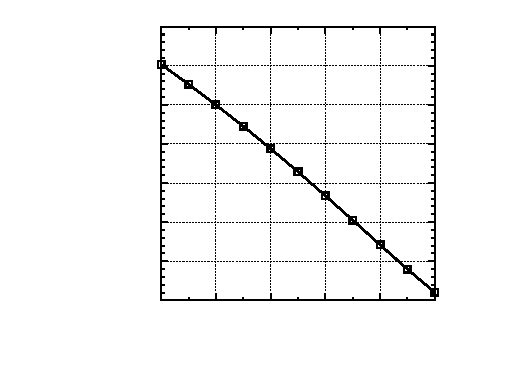
\includegraphics{figures/clh-en/clh-en}}%
    \gplfronttext
  \end{picture}%
\endgroup
\hspace*{-1.3cm}% GNUPLOT: LaTeX picture with Postscript
\begingroup
  \makeatletter
  \providecommand\color[2][]{%
    \GenericError{(gnuplot) \space\space\space\@spaces}{%
      Package color not loaded in conjunction with
      terminal option `colourtext'%
    }{See the gnuplot documentation for explanation.%
    }{Either use 'blacktext' in gnuplot or load the package
      color.sty in LaTeX.}%
    \renewcommand\color[2][]{}%
  }%
  \providecommand\includegraphics[2][]{%
    \GenericError{(gnuplot) \space\space\space\@spaces}{%
      Package graphicx or graphics not loaded%
    }{See the gnuplot documentation for explanation.%
    }{The gnuplot epslatex terminal needs graphicx.sty or graphics.sty.}%
    \renewcommand\includegraphics[2][]{}%
  }%
  \providecommand\rotatebox[2]{#2}%
  \@ifundefined{ifGPcolor}{%
    \newif\ifGPcolor
    \GPcolortrue
  }{}%
  \@ifundefined{ifGPblacktext}{%
    \newif\ifGPblacktext
    \GPblacktextfalse
  }{}%
  % define a \g@addto@macro without @ in the name:
  \let\gplgaddtomacro\g@addto@macro
  % define empty templates for all commands taking text:
  \gdef\gplbacktext{}%
  \gdef\gplfronttext{}%
  \makeatother
  \ifGPblacktext
    % no textcolor at all
    \def\colorrgb#1{}%
    \def\colorgray#1{}%
  \else
    % gray or color?
    \ifGPcolor
      \def\colorrgb#1{\color[rgb]{#1}}%
      \def\colorgray#1{\color[gray]{#1}}%
      \expandafter\def\csname LTw\endcsname{\color{white}}%
      \expandafter\def\csname LTb\endcsname{\color{black}}%
      \expandafter\def\csname LTa\endcsname{\color{black}}%
      \expandafter\def\csname LT0\endcsname{\color[rgb]{1,0,0}}%
      \expandafter\def\csname LT1\endcsname{\color[rgb]{0,1,0}}%
      \expandafter\def\csname LT2\endcsname{\color[rgb]{0,0,1}}%
      \expandafter\def\csname LT3\endcsname{\color[rgb]{1,0,1}}%
      \expandafter\def\csname LT4\endcsname{\color[rgb]{0,1,1}}%
      \expandafter\def\csname LT5\endcsname{\color[rgb]{1,1,0}}%
      \expandafter\def\csname LT6\endcsname{\color[rgb]{0,0,0}}%
      \expandafter\def\csname LT7\endcsname{\color[rgb]{1,0.3,0}}%
      \expandafter\def\csname LT8\endcsname{\color[rgb]{0.5,0.5,0.5}}%
    \else
      % gray
      \def\colorrgb#1{\color{black}}%
      \def\colorgray#1{\color[gray]{#1}}%
      \expandafter\def\csname LTw\endcsname{\color{white}}%
      \expandafter\def\csname LTb\endcsname{\color{black}}%
      \expandafter\def\csname LTa\endcsname{\color{black}}%
      \expandafter\def\csname LT0\endcsname{\color{black}}%
      \expandafter\def\csname LT1\endcsname{\color{black}}%
      \expandafter\def\csname LT2\endcsname{\color{black}}%
      \expandafter\def\csname LT3\endcsname{\color{black}}%
      \expandafter\def\csname LT4\endcsname{\color{black}}%
      \expandafter\def\csname LT5\endcsname{\color{black}}%
      \expandafter\def\csname LT6\endcsname{\color{black}}%
      \expandafter\def\csname LT7\endcsname{\color{black}}%
      \expandafter\def\csname LT8\endcsname{\color{black}}%
    \fi
  \fi
  \setlength{\unitlength}{0.0500bp}%
  \begin{picture}(5040.00,3772.00)%
    \gplgaddtomacro\gplbacktext{%
      \csname LTb\endcsname%
      \put(1481,880){\makebox(0,0)[r]{\strut{}-0.2}}%
      \csname LTb\endcsname%
      \put(1481,1208){\makebox(0,0)[r]{\strut{}-0.15}}%
      \csname LTb\endcsname%
      \put(1481,1537){\makebox(0,0)[r]{\strut{}-0.1}}%
      \csname LTb\endcsname%
      \put(1481,1865){\makebox(0,0)[r]{\strut{}-0.05}}%
      \csname LTb\endcsname%
      \put(1481,2194){\makebox(0,0)[r]{\strut{} 0}}%
      \csname LTb\endcsname%
      \put(1481,2522){\makebox(0,0)[r]{\strut{} 0.05}}%
      \csname LTb\endcsname%
      \put(1481,2850){\makebox(0,0)[r]{\strut{} 0.1}}%
      \csname LTb\endcsname%
      \put(1481,3179){\makebox(0,0)[r]{\strut{} 0.15}}%
      \csname LTb\endcsname%
      \put(1481,3507){\makebox(0,0)[r]{\strut{} 0.2}}%
      \csname LTb\endcsname%
      \put(1613,660){\makebox(0,0){\strut{} 0}}%
      \csname LTb\endcsname%
      \put(2138,660){\makebox(0,0){\strut{} 0.2}}%
      \csname LTb\endcsname%
      \put(2664,660){\makebox(0,0){\strut{} 0.4}}%
      \csname LTb\endcsname%
      \put(3189,660){\makebox(0,0){\strut{} 0.6}}%
      \csname LTb\endcsname%
      \put(3715,660){\makebox(0,0){\strut{} 0.8}}%
      \csname LTb\endcsname%
      \put(4240,660){\makebox(0,0){\strut{} 1}}%
      \put(579,2193){\rotatebox{-270}{\makebox(0,0){\strut{}charge}}}%
      \put(2926,330){\makebox(0,0){\strut{}$\lambda$}}%
    }%
    \gplgaddtomacro\gplfronttext{%
      \csname LTb\endcsname%
      \put(3253,3334){\makebox(0,0)[r]{\strut{}Cl $\rightarrow$ H}}%
      \csname LTb\endcsname%
      \put(3253,3114){\makebox(0,0)[r]{\strut{}C}}%
    }%
    \gplbacktext
    \put(0,0){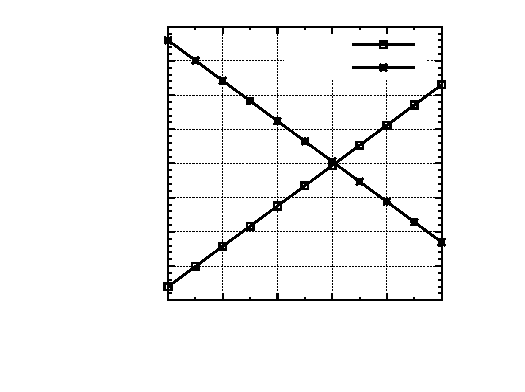
\includegraphics{figures/clh-charge/clh-charge}}%
    \gplfronttext
  \end{picture}%
\endgroup
\\
% GNUPLOT: LaTeX picture with Postscript
\begingroup
  \makeatletter
  \providecommand\color[2][]{%
    \GenericError{(gnuplot) \space\space\space\@spaces}{%
      Package color not loaded in conjunction with
      terminal option `colourtext'%
    }{See the gnuplot documentation for explanation.%
    }{Either use 'blacktext' in gnuplot or load the package
      color.sty in LaTeX.}%
    \renewcommand\color[2][]{}%
  }%
  \providecommand\includegraphics[2][]{%
    \GenericError{(gnuplot) \space\space\space\@spaces}{%
      Package graphicx or graphics not loaded%
    }{See the gnuplot documentation for explanation.%
    }{The gnuplot epslatex terminal needs graphicx.sty or graphics.sty.}%
    \renewcommand\includegraphics[2][]{}%
  }%
  \providecommand\rotatebox[2]{#2}%
  \@ifundefined{ifGPcolor}{%
    \newif\ifGPcolor
    \GPcolortrue
  }{}%
  \@ifundefined{ifGPblacktext}{%
    \newif\ifGPblacktext
    \GPblacktextfalse
  }{}%
  % define a \g@addto@macro without @ in the name:
  \let\gplgaddtomacro\g@addto@macro
  % define empty templates for all commands taking text:
  \gdef\gplbacktext{}%
  \gdef\gplfronttext{}%
  \makeatother
  \ifGPblacktext
    % no textcolor at all
    \def\colorrgb#1{}%
    \def\colorgray#1{}%
  \else
    % gray or color?
    \ifGPcolor
      \def\colorrgb#1{\color[rgb]{#1}}%
      \def\colorgray#1{\color[gray]{#1}}%
      \expandafter\def\csname LTw\endcsname{\color{white}}%
      \expandafter\def\csname LTb\endcsname{\color{black}}%
      \expandafter\def\csname LTa\endcsname{\color{black}}%
      \expandafter\def\csname LT0\endcsname{\color[rgb]{1,0,0}}%
      \expandafter\def\csname LT1\endcsname{\color[rgb]{0,1,0}}%
      \expandafter\def\csname LT2\endcsname{\color[rgb]{0,0,1}}%
      \expandafter\def\csname LT3\endcsname{\color[rgb]{1,0,1}}%
      \expandafter\def\csname LT4\endcsname{\color[rgb]{0,1,1}}%
      \expandafter\def\csname LT5\endcsname{\color[rgb]{1,1,0}}%
      \expandafter\def\csname LT6\endcsname{\color[rgb]{0,0,0}}%
      \expandafter\def\csname LT7\endcsname{\color[rgb]{1,0.3,0}}%
      \expandafter\def\csname LT8\endcsname{\color[rgb]{0.5,0.5,0.5}}%
    \else
      % gray
      \def\colorrgb#1{\color{black}}%
      \def\colorgray#1{\color[gray]{#1}}%
      \expandafter\def\csname LTw\endcsname{\color{white}}%
      \expandafter\def\csname LTb\endcsname{\color{black}}%
      \expandafter\def\csname LTa\endcsname{\color{black}}%
      \expandafter\def\csname LT0\endcsname{\color{black}}%
      \expandafter\def\csname LT1\endcsname{\color{black}}%
      \expandafter\def\csname LT2\endcsname{\color{black}}%
      \expandafter\def\csname LT3\endcsname{\color{black}}%
      \expandafter\def\csname LT4\endcsname{\color{black}}%
      \expandafter\def\csname LT5\endcsname{\color{black}}%
      \expandafter\def\csname LT6\endcsname{\color{black}}%
      \expandafter\def\csname LT7\endcsname{\color{black}}%
      \expandafter\def\csname LT8\endcsname{\color{black}}%
    \fi
  \fi
  \setlength{\unitlength}{0.0500bp}%
  \begin{picture}(5040.00,3772.00)%
    \gplgaddtomacro\gplbacktext{%
      \csname LTb\endcsname%
      \put(1349,880){\makebox(0,0)[r]{\strut{} 2}}%
      \csname LTb\endcsname%
      \put(1349,1208){\makebox(0,0)[r]{\strut{} 4}}%
      \csname LTb\endcsname%
      \put(1349,1537){\makebox(0,0)[r]{\strut{} 6}}%
      \csname LTb\endcsname%
      \put(1349,1865){\makebox(0,0)[r]{\strut{} 8}}%
      \csname LTb\endcsname%
      \put(1349,2194){\makebox(0,0)[r]{\strut{} 10}}%
      \csname LTb\endcsname%
      \put(1349,2522){\makebox(0,0)[r]{\strut{} 12}}%
      \csname LTb\endcsname%
      \put(1349,2850){\makebox(0,0)[r]{\strut{} 14}}%
      \csname LTb\endcsname%
      \put(1349,3179){\makebox(0,0)[r]{\strut{} 16}}%
      \csname LTb\endcsname%
      \put(1349,3507){\makebox(0,0)[r]{\strut{} 18}}%
      \csname LTb\endcsname%
      \put(1481,660){\makebox(0,0){\strut{} 0}}%
      \csname LTb\endcsname%
      \put(2006,660){\makebox(0,0){\strut{} 0.2}}%
      \csname LTb\endcsname%
      \put(2532,660){\makebox(0,0){\strut{} 0.4}}%
      \csname LTb\endcsname%
      \put(3057,660){\makebox(0,0){\strut{} 0.6}}%
      \csname LTb\endcsname%
      \put(3583,660){\makebox(0,0){\strut{} 0.8}}%
      \csname LTb\endcsname%
      \put(4108,660){\makebox(0,0){\strut{} 1}}%
      \csname LTb\endcsname%
      \put(711,2193){\rotatebox{-270}{\makebox(0,0){\strut{}volume (\AA$^{3}$)}}}%
      \put(2794,330){\makebox(0,0){\strut{}$\lambda$}}%
    }%
    \gplgaddtomacro\gplfronttext{%
      \csname LTb\endcsname%
      \put(3121,3334){\makebox(0,0)[r]{\strut{}Cl $\rightarrow$ H}}%
      \csname LTb\endcsname%
      \put(3121,3114){\makebox(0,0)[r]{\strut{}C}}%
    }%
    \gplbacktext
    \put(0,0){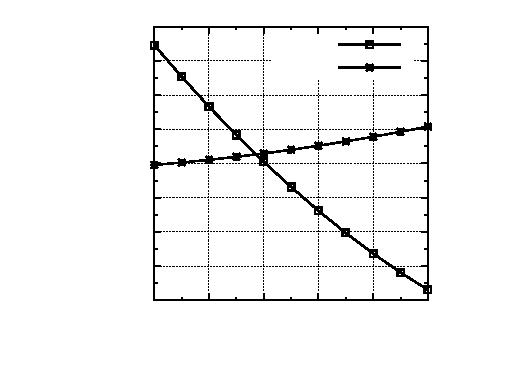
\includegraphics{figures/clh-vol/clh-vol}}%
    \gplfronttext
  \end{picture}%
\endgroup
\hspace*{-1.3cm}% GNUPLOT: LaTeX picture with Postscript
\begingroup
  \makeatletter
  \providecommand\color[2][]{%
    \GenericError{(gnuplot) \space\space\space\@spaces}{%
      Package color not loaded in conjunction with
      terminal option `colourtext'%
    }{See the gnuplot documentation for explanation.%
    }{Either use 'blacktext' in gnuplot or load the package
      color.sty in LaTeX.}%
    \renewcommand\color[2][]{}%
  }%
  \providecommand\includegraphics[2][]{%
    \GenericError{(gnuplot) \space\space\space\@spaces}{%
      Package graphicx or graphics not loaded%
    }{See the gnuplot documentation for explanation.%
    }{The gnuplot epslatex terminal needs graphicx.sty or graphics.sty.}%
    \renewcommand\includegraphics[2][]{}%
  }%
  \providecommand\rotatebox[2]{#2}%
  \@ifundefined{ifGPcolor}{%
    \newif\ifGPcolor
    \GPcolortrue
  }{}%
  \@ifundefined{ifGPblacktext}{%
    \newif\ifGPblacktext
    \GPblacktextfalse
  }{}%
  % define a \g@addto@macro without @ in the name:
  \let\gplgaddtomacro\g@addto@macro
  % define empty templates for all commands taking text:
  \gdef\gplbacktext{}%
  \gdef\gplfronttext{}%
  \makeatother
  \ifGPblacktext
    % no textcolor at all
    \def\colorrgb#1{}%
    \def\colorgray#1{}%
  \else
    % gray or color?
    \ifGPcolor
      \def\colorrgb#1{\color[rgb]{#1}}%
      \def\colorgray#1{\color[gray]{#1}}%
      \expandafter\def\csname LTw\endcsname{\color{white}}%
      \expandafter\def\csname LTb\endcsname{\color{black}}%
      \expandafter\def\csname LTa\endcsname{\color{black}}%
      \expandafter\def\csname LT0\endcsname{\color[rgb]{1,0,0}}%
      \expandafter\def\csname LT1\endcsname{\color[rgb]{0,1,0}}%
      \expandafter\def\csname LT2\endcsname{\color[rgb]{0,0,1}}%
      \expandafter\def\csname LT3\endcsname{\color[rgb]{1,0,1}}%
      \expandafter\def\csname LT4\endcsname{\color[rgb]{0,1,1}}%
      \expandafter\def\csname LT5\endcsname{\color[rgb]{1,1,0}}%
      \expandafter\def\csname LT6\endcsname{\color[rgb]{0,0,0}}%
      \expandafter\def\csname LT7\endcsname{\color[rgb]{1,0.3,0}}%
      \expandafter\def\csname LT8\endcsname{\color[rgb]{0.5,0.5,0.5}}%
    \else
      % gray
      \def\colorrgb#1{\color{black}}%
      \def\colorgray#1{\color[gray]{#1}}%
      \expandafter\def\csname LTw\endcsname{\color{white}}%
      \expandafter\def\csname LTb\endcsname{\color{black}}%
      \expandafter\def\csname LTa\endcsname{\color{black}}%
      \expandafter\def\csname LT0\endcsname{\color{black}}%
      \expandafter\def\csname LT1\endcsname{\color{black}}%
      \expandafter\def\csname LT2\endcsname{\color{black}}%
      \expandafter\def\csname LT3\endcsname{\color{black}}%
      \expandafter\def\csname LT4\endcsname{\color{black}}%
      \expandafter\def\csname LT5\endcsname{\color{black}}%
      \expandafter\def\csname LT6\endcsname{\color{black}}%
      \expandafter\def\csname LT7\endcsname{\color{black}}%
      \expandafter\def\csname LT8\endcsname{\color{black}}%
    \fi
  \fi
  \setlength{\unitlength}{0.0500bp}%
  \begin{picture}(5040.00,3772.00)%
    \gplgaddtomacro\gplbacktext{%
      \csname LTb\endcsname%
      \put(1415,1099){\makebox(0,0)[r]{\strut{}-120}}%
      \csname LTb\endcsname%
      \put(1415,1537){\makebox(0,0)[r]{\strut{}-110}}%
      \csname LTb\endcsname%
      \put(1415,1975){\makebox(0,0)[r]{\strut{}-100}}%
      \csname LTb\endcsname%
      \put(1415,2412){\makebox(0,0)[r]{\strut{}-90}}%
      \csname LTb\endcsname%
      \put(1415,2850){\makebox(0,0)[r]{\strut{}-80}}%
      \csname LTb\endcsname%
      \put(1415,3288){\makebox(0,0)[r]{\strut{}-70}}%
      \csname LTb\endcsname%
      \put(1547,660){\makebox(0,0){\strut{} 0}}%
      \csname LTb\endcsname%
      \put(2072,660){\makebox(0,0){\strut{} 0.2}}%
      \csname LTb\endcsname%
      \put(2598,660){\makebox(0,0){\strut{} 0.4}}%
      \csname LTb\endcsname%
      \put(3123,660){\makebox(0,0){\strut{} 0.6}}%
      \csname LTb\endcsname%
      \put(3649,660){\makebox(0,0){\strut{} 0.8}}%
      \csname LTb\endcsname%
      \put(4174,660){\makebox(0,0){\strut{} 1}}%
      \csname LTb\endcsname%
      \put(645,2193){\rotatebox{-270}{\makebox(0,0){\strut{}$G^\prime_{\textrm{pol},i}$}}}%
      \put(2860,330){\makebox(0,0){\strut{}$\lambda$}}%
    }%
    \gplgaddtomacro\gplfronttext{%
      \csname LTb\endcsname%
      \put(3187,3334){\makebox(0,0)[r]{\strut{}Cl $\rightarrow$ H}}%
      \csname LTb\endcsname%
      \put(3187,3114){\makebox(0,0)[r]{\strut{}C}}%
    }%
    \gplbacktext
    \put(0,0){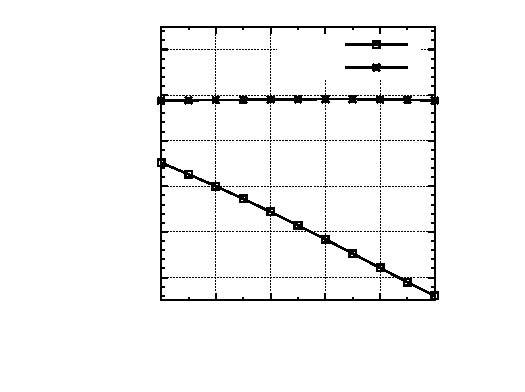
\includegraphics{figures/clh-pol/clh-pol}}%
    \gplfronttext
  \end{picture}%
\endgroup

\caption{The Born energy and components thereof for the perturbation of chlorobenzene to benzene. Top left: energy trajectory; top right: charge trajectories; bottom left: volume trajectories; bottom right: electrostatic trajectories.}
\label{clh}
\end{figure}

PhCl $\longrightarrow$ PhH. Results for the perturbation of chlorobenzene to benzene are given in \cref{clh}. Key atoms were determined to be the chlorine and the carbon to which the chlorine was attached. Given the aforementioned challenges with calculating van der Waals overlap in FEP, this example was particularly interesting as a test case because of the large differences in charge and volume between the initial and final state. All trajectories were smooth and consistent throughout the course of the perturbation. The charge trajectory (\cref{clh}, top right) reflected a reversal in charge in perturbing chlorine to hydrogen, consistent with the charge distribution observed for benzene. A similar reversal was seen in the case of atomic volumes, \cref{clh}, bottom left. A dramatic decrease in atomic volume was observed for the perturbation of chlorine to hydrogen, with concomitant increase in effective atomic volume for the attached carbon, owing to a decrease in van der Waals overlap. Electrostatic contribution (\cref{clh}, bottom right) also behaved as expected, and the resulting total Born energy followed a smooth arch with a maximum change in energy at $\lambda = 0.5$ and an overall $\Delta G_{ \textrm{Born}}$ of $+0.124$ kcal/mol for the perturbation.

\begin{figure}[t!]
\centering
PhCN $\longrightarrow$ PhF\\
% GNUPLOT: LaTeX picture with Postscript
\begingroup
  \makeatletter
  \providecommand\color[2][]{%
    \GenericError{(gnuplot) \space\space\space\@spaces}{%
      Package color not loaded in conjunction with
      terminal option `colourtext'%
    }{See the gnuplot documentation for explanation.%
    }{Either use 'blacktext' in gnuplot or load the package
      color.sty in LaTeX.}%
    \renewcommand\color[2][]{}%
  }%
  \providecommand\includegraphics[2][]{%
    \GenericError{(gnuplot) \space\space\space\@spaces}{%
      Package graphicx or graphics not loaded%
    }{See the gnuplot documentation for explanation.%
    }{The gnuplot epslatex terminal needs graphicx.sty or graphics.sty.}%
    \renewcommand\includegraphics[2][]{}%
  }%
  \providecommand\rotatebox[2]{#2}%
  \@ifundefined{ifGPcolor}{%
    \newif\ifGPcolor
    \GPcolortrue
  }{}%
  \@ifundefined{ifGPblacktext}{%
    \newif\ifGPblacktext
    \GPblacktextfalse
  }{}%
  % define a \g@addto@macro without @ in the name:
  \let\gplgaddtomacro\g@addto@macro
  % define empty templates for all commands taking text:
  \gdef\gplbacktext{}%
  \gdef\gplfronttext{}%
  \makeatother
  \ifGPblacktext
    % no textcolor at all
    \def\colorrgb#1{}%
    \def\colorgray#1{}%
  \else
    % gray or color?
    \ifGPcolor
      \def\colorrgb#1{\color[rgb]{#1}}%
      \def\colorgray#1{\color[gray]{#1}}%
      \expandafter\def\csname LTw\endcsname{\color{white}}%
      \expandafter\def\csname LTb\endcsname{\color{black}}%
      \expandafter\def\csname LTa\endcsname{\color{black}}%
      \expandafter\def\csname LT0\endcsname{\color[rgb]{1,0,0}}%
      \expandafter\def\csname LT1\endcsname{\color[rgb]{0,1,0}}%
      \expandafter\def\csname LT2\endcsname{\color[rgb]{0,0,1}}%
      \expandafter\def\csname LT3\endcsname{\color[rgb]{1,0,1}}%
      \expandafter\def\csname LT4\endcsname{\color[rgb]{0,1,1}}%
      \expandafter\def\csname LT5\endcsname{\color[rgb]{1,1,0}}%
      \expandafter\def\csname LT6\endcsname{\color[rgb]{0,0,0}}%
      \expandafter\def\csname LT7\endcsname{\color[rgb]{1,0.3,0}}%
      \expandafter\def\csname LT8\endcsname{\color[rgb]{0.5,0.5,0.5}}%
    \else
      % gray
      \def\colorrgb#1{\color{black}}%
      \def\colorgray#1{\color[gray]{#1}}%
      \expandafter\def\csname LTw\endcsname{\color{white}}%
      \expandafter\def\csname LTb\endcsname{\color{black}}%
      \expandafter\def\csname LTa\endcsname{\color{black}}%
      \expandafter\def\csname LT0\endcsname{\color{black}}%
      \expandafter\def\csname LT1\endcsname{\color{black}}%
      \expandafter\def\csname LT2\endcsname{\color{black}}%
      \expandafter\def\csname LT3\endcsname{\color{black}}%
      \expandafter\def\csname LT4\endcsname{\color{black}}%
      \expandafter\def\csname LT5\endcsname{\color{black}}%
      \expandafter\def\csname LT6\endcsname{\color{black}}%
      \expandafter\def\csname LT7\endcsname{\color{black}}%
      \expandafter\def\csname LT8\endcsname{\color{black}}%
    \fi
  \fi
  \setlength{\unitlength}{0.0500bp}%
  \begin{picture}(5040.00,3772.00)%
    \gplgaddtomacro\gplbacktext{%
      \csname LTb\endcsname%
      \put(1415,880){\makebox(0,0)[r]{\strut{}-6}}%
      \csname LTb\endcsname%
      \put(1415,1172){\makebox(0,0)[r]{\strut{}-5.5}}%
      \csname LTb\endcsname%
      \put(1415,1464){\makebox(0,0)[r]{\strut{}-5}}%
      \csname LTb\endcsname%
      \put(1415,1756){\makebox(0,0)[r]{\strut{}-4.5}}%
      \csname LTb\endcsname%
      \put(1415,2048){\makebox(0,0)[r]{\strut{}-4}}%
      \csname LTb\endcsname%
      \put(1415,2339){\makebox(0,0)[r]{\strut{}-3.5}}%
      \csname LTb\endcsname%
      \put(1415,2631){\makebox(0,0)[r]{\strut{}-3}}%
      \csname LTb\endcsname%
      \put(1415,2923){\makebox(0,0)[r]{\strut{}-2.5}}%
      \csname LTb\endcsname%
      \put(1415,3215){\makebox(0,0)[r]{\strut{}-2}}%
      \csname LTb\endcsname%
      \put(1415,3507){\makebox(0,0)[r]{\strut{}-1.5}}%
      \csname LTb\endcsname%
      \put(1547,660){\makebox(0,0){\strut{} 0}}%
      \csname LTb\endcsname%
      \put(2072,660){\makebox(0,0){\strut{} 0.2}}%
      \csname LTb\endcsname%
      \put(2598,660){\makebox(0,0){\strut{} 0.4}}%
      \csname LTb\endcsname%
      \put(3123,660){\makebox(0,0){\strut{} 0.6}}%
      \csname LTb\endcsname%
      \put(3649,660){\makebox(0,0){\strut{} 0.8}}%
      \csname LTb\endcsname%
      \put(4174,660){\makebox(0,0){\strut{} 1}}%
      \csname LTb\endcsname%
      \put(645,2193){\rotatebox{-270}{\makebox(0,0){\strut{}Born energy (kcal/mol)}}}%
      \put(2860,330){\makebox(0,0){\strut{}$\lambda$}}%
    }%
    \gplgaddtomacro\gplfronttext{%
    }%
    \gplbacktext
    \put(0,0){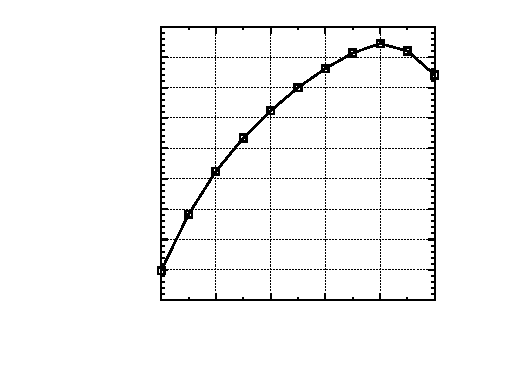
\includegraphics{figures/cnf-en/cnf-en}}%
    \gplfronttext
  \end{picture}%
\endgroup
\hspace*{-1.3cm}% GNUPLOT: LaTeX picture with Postscript
\begingroup
  \makeatletter
  \providecommand\color[2][]{%
    \GenericError{(gnuplot) \space\space\space\@spaces}{%
      Package color not loaded in conjunction with
      terminal option `colourtext'%
    }{See the gnuplot documentation for explanation.%
    }{Either use 'blacktext' in gnuplot or load the package
      color.sty in LaTeX.}%
    \renewcommand\color[2][]{}%
  }%
  \providecommand\includegraphics[2][]{%
    \GenericError{(gnuplot) \space\space\space\@spaces}{%
      Package graphicx or graphics not loaded%
    }{See the gnuplot documentation for explanation.%
    }{The gnuplot epslatex terminal needs graphicx.sty or graphics.sty.}%
    \renewcommand\includegraphics[2][]{}%
  }%
  \providecommand\rotatebox[2]{#2}%
  \@ifundefined{ifGPcolor}{%
    \newif\ifGPcolor
    \GPcolortrue
  }{}%
  \@ifundefined{ifGPblacktext}{%
    \newif\ifGPblacktext
    \GPblacktextfalse
  }{}%
  % define a \g@addto@macro without @ in the name:
  \let\gplgaddtomacro\g@addto@macro
  % define empty templates for all commands taking text:
  \gdef\gplbacktext{}%
  \gdef\gplfronttext{}%
  \makeatother
  \ifGPblacktext
    % no textcolor at all
    \def\colorrgb#1{}%
    \def\colorgray#1{}%
  \else
    % gray or color?
    \ifGPcolor
      \def\colorrgb#1{\color[rgb]{#1}}%
      \def\colorgray#1{\color[gray]{#1}}%
      \expandafter\def\csname LTw\endcsname{\color{white}}%
      \expandafter\def\csname LTb\endcsname{\color{black}}%
      \expandafter\def\csname LTa\endcsname{\color{black}}%
      \expandafter\def\csname LT0\endcsname{\color[rgb]{1,0,0}}%
      \expandafter\def\csname LT1\endcsname{\color[rgb]{0,1,0}}%
      \expandafter\def\csname LT2\endcsname{\color[rgb]{0,0,1}}%
      \expandafter\def\csname LT3\endcsname{\color[rgb]{1,0,1}}%
      \expandafter\def\csname LT4\endcsname{\color[rgb]{0,1,1}}%
      \expandafter\def\csname LT5\endcsname{\color[rgb]{1,1,0}}%
      \expandafter\def\csname LT6\endcsname{\color[rgb]{0,0,0}}%
      \expandafter\def\csname LT7\endcsname{\color[rgb]{1,0.3,0}}%
      \expandafter\def\csname LT8\endcsname{\color[rgb]{0.5,0.5,0.5}}%
    \else
      % gray
      \def\colorrgb#1{\color{black}}%
      \def\colorgray#1{\color[gray]{#1}}%
      \expandafter\def\csname LTw\endcsname{\color{white}}%
      \expandafter\def\csname LTb\endcsname{\color{black}}%
      \expandafter\def\csname LTa\endcsname{\color{black}}%
      \expandafter\def\csname LT0\endcsname{\color{black}}%
      \expandafter\def\csname LT1\endcsname{\color{black}}%
      \expandafter\def\csname LT2\endcsname{\color{black}}%
      \expandafter\def\csname LT3\endcsname{\color{black}}%
      \expandafter\def\csname LT4\endcsname{\color{black}}%
      \expandafter\def\csname LT5\endcsname{\color{black}}%
      \expandafter\def\csname LT6\endcsname{\color{black}}%
      \expandafter\def\csname LT7\endcsname{\color{black}}%
      \expandafter\def\csname LT8\endcsname{\color{black}}%
    \fi
  \fi
  \setlength{\unitlength}{0.0500bp}%
  \begin{picture}(5040.00,3772.00)%
    \gplgaddtomacro\gplbacktext{%
      \csname LTb\endcsname%
      \put(1415,1099){\makebox(0,0)[r]{\strut{}-0.4}}%
      \csname LTb\endcsname%
      \put(1415,1537){\makebox(0,0)[r]{\strut{}-0.2}}%
      \csname LTb\endcsname%
      \put(1415,1975){\makebox(0,0)[r]{\strut{} 0}}%
      \csname LTb\endcsname%
      \put(1415,2412){\makebox(0,0)[r]{\strut{} 0.2}}%
      \csname LTb\endcsname%
      \put(1415,2850){\makebox(0,0)[r]{\strut{} 0.4}}%
      \csname LTb\endcsname%
      \put(1415,3288){\makebox(0,0)[r]{\strut{} 0.6}}%
      \csname LTb\endcsname%
      \put(1547,660){\makebox(0,0){\strut{} 0}}%
      \csname LTb\endcsname%
      \put(2072,660){\makebox(0,0){\strut{} 0.2}}%
      \csname LTb\endcsname%
      \put(2598,660){\makebox(0,0){\strut{} 0.4}}%
      \csname LTb\endcsname%
      \put(3123,660){\makebox(0,0){\strut{} 0.6}}%
      \csname LTb\endcsname%
      \put(3649,660){\makebox(0,0){\strut{} 0.8}}%
      \csname LTb\endcsname%
      \put(4174,660){\makebox(0,0){\strut{} 1}}%
      \put(645,2193){\rotatebox{-270}{\makebox(0,0){\strut{}charge}}}%
      \put(2860,330){\makebox(0,0){\strut{}$\lambda$}}%
    }%
    \gplgaddtomacro\gplfronttext{%
      \csname LTb\endcsname%
      \put(3187,3334){\makebox(0,0)[r]{\strut{}C $\rightarrow$ F}}%
      \csname LTb\endcsname%
      \put(3187,3114){\makebox(0,0)[r]{\strut{}C}}%
      \csname LTb\endcsname%
      \put(3187,2894){\makebox(0,0)[r]{\strut{}N $\rightarrow$ Dummy}}%
    }%
    \gplbacktext
    \put(0,0){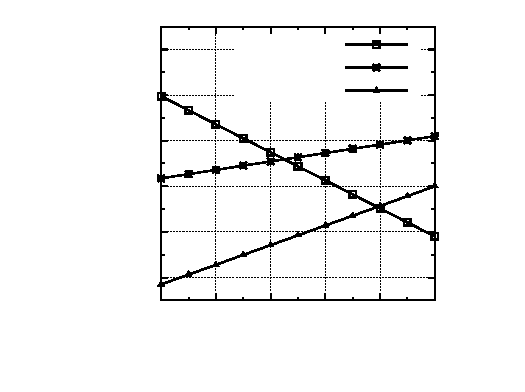
\includegraphics{figures/cnf-charge/cnf-charge}}%
    \gplfronttext
  \end{picture}%
\endgroup
\\
% GNUPLOT: LaTeX picture with Postscript
\begingroup
  \makeatletter
  \providecommand\color[2][]{%
    \GenericError{(gnuplot) \space\space\space\@spaces}{%
      Package color not loaded in conjunction with
      terminal option `colourtext'%
    }{See the gnuplot documentation for explanation.%
    }{Either use 'blacktext' in gnuplot or load the package
      color.sty in LaTeX.}%
    \renewcommand\color[2][]{}%
  }%
  \providecommand\includegraphics[2][]{%
    \GenericError{(gnuplot) \space\space\space\@spaces}{%
      Package graphicx or graphics not loaded%
    }{See the gnuplot documentation for explanation.%
    }{The gnuplot epslatex terminal needs graphicx.sty or graphics.sty.}%
    \renewcommand\includegraphics[2][]{}%
  }%
  \providecommand\rotatebox[2]{#2}%
  \@ifundefined{ifGPcolor}{%
    \newif\ifGPcolor
    \GPcolortrue
  }{}%
  \@ifundefined{ifGPblacktext}{%
    \newif\ifGPblacktext
    \GPblacktextfalse
  }{}%
  % define a \g@addto@macro without @ in the name:
  \let\gplgaddtomacro\g@addto@macro
  % define empty templates for all commands taking text:
  \gdef\gplbacktext{}%
  \gdef\gplfronttext{}%
  \makeatother
  \ifGPblacktext
    % no textcolor at all
    \def\colorrgb#1{}%
    \def\colorgray#1{}%
  \else
    % gray or color?
    \ifGPcolor
      \def\colorrgb#1{\color[rgb]{#1}}%
      \def\colorgray#1{\color[gray]{#1}}%
      \expandafter\def\csname LTw\endcsname{\color{white}}%
      \expandafter\def\csname LTb\endcsname{\color{black}}%
      \expandafter\def\csname LTa\endcsname{\color{black}}%
      \expandafter\def\csname LT0\endcsname{\color[rgb]{1,0,0}}%
      \expandafter\def\csname LT1\endcsname{\color[rgb]{0,1,0}}%
      \expandafter\def\csname LT2\endcsname{\color[rgb]{0,0,1}}%
      \expandafter\def\csname LT3\endcsname{\color[rgb]{1,0,1}}%
      \expandafter\def\csname LT4\endcsname{\color[rgb]{0,1,1}}%
      \expandafter\def\csname LT5\endcsname{\color[rgb]{1,1,0}}%
      \expandafter\def\csname LT6\endcsname{\color[rgb]{0,0,0}}%
      \expandafter\def\csname LT7\endcsname{\color[rgb]{1,0.3,0}}%
      \expandafter\def\csname LT8\endcsname{\color[rgb]{0.5,0.5,0.5}}%
    \else
      % gray
      \def\colorrgb#1{\color{black}}%
      \def\colorgray#1{\color[gray]{#1}}%
      \expandafter\def\csname LTw\endcsname{\color{white}}%
      \expandafter\def\csname LTb\endcsname{\color{black}}%
      \expandafter\def\csname LTa\endcsname{\color{black}}%
      \expandafter\def\csname LT0\endcsname{\color{black}}%
      \expandafter\def\csname LT1\endcsname{\color{black}}%
      \expandafter\def\csname LT2\endcsname{\color{black}}%
      \expandafter\def\csname LT3\endcsname{\color{black}}%
      \expandafter\def\csname LT4\endcsname{\color{black}}%
      \expandafter\def\csname LT5\endcsname{\color{black}}%
      \expandafter\def\csname LT6\endcsname{\color{black}}%
      \expandafter\def\csname LT7\endcsname{\color{black}}%
      \expandafter\def\csname LT8\endcsname{\color{black}}%
    \fi
  \fi
  \setlength{\unitlength}{0.0500bp}%
  \begin{picture}(5040.00,3772.00)%
    \gplgaddtomacro\gplbacktext{%
      \csname LTb\endcsname%
      \put(1349,880){\makebox(0,0)[r]{\strut{} 0}}%
      \csname LTb\endcsname%
      \put(1349,1255){\makebox(0,0)[r]{\strut{} 5}}%
      \csname LTb\endcsname%
      \put(1349,1631){\makebox(0,0)[r]{\strut{} 10}}%
      \csname LTb\endcsname%
      \put(1349,2006){\makebox(0,0)[r]{\strut{} 15}}%
      \csname LTb\endcsname%
      \put(1349,2381){\makebox(0,0)[r]{\strut{} 20}}%
      \csname LTb\endcsname%
      \put(1349,2756){\makebox(0,0)[r]{\strut{} 25}}%
      \csname LTb\endcsname%
      \put(1349,3132){\makebox(0,0)[r]{\strut{} 30}}%
      \csname LTb\endcsname%
      \put(1349,3507){\makebox(0,0)[r]{\strut{} 35}}%
      \csname LTb\endcsname%
      \put(1481,660){\makebox(0,0){\strut{} 0}}%
      \csname LTb\endcsname%
      \put(2006,660){\makebox(0,0){\strut{} 0.2}}%
      \csname LTb\endcsname%
      \put(2532,660){\makebox(0,0){\strut{} 0.4}}%
      \csname LTb\endcsname%
      \put(3057,660){\makebox(0,0){\strut{} 0.6}}%
      \csname LTb\endcsname%
      \put(3583,660){\makebox(0,0){\strut{} 0.8}}%
      \csname LTb\endcsname%
      \put(4108,660){\makebox(0,0){\strut{} 1}}%
      \csname LTb\endcsname%
      \put(711,2193){\rotatebox{-270}{\makebox(0,0){\strut{}volume (\AA$^{3}$)}}}%
      \put(2794,330){\makebox(0,0){\strut{}$\lambda$}}%
    }%
    \gplgaddtomacro\gplfronttext{%
      \csname LTb\endcsname%
      \put(3121,3334){\makebox(0,0)[r]{\strut{}C $\rightarrow$ F}}%
      \csname LTb\endcsname%
      \put(3121,3114){\makebox(0,0)[r]{\strut{}C}}%
      \csname LTb\endcsname%
      \put(3121,2894){\makebox(0,0)[r]{\strut{}N $\rightarrow$ Dummy}}%
    }%
    \gplbacktext
    \put(0,0){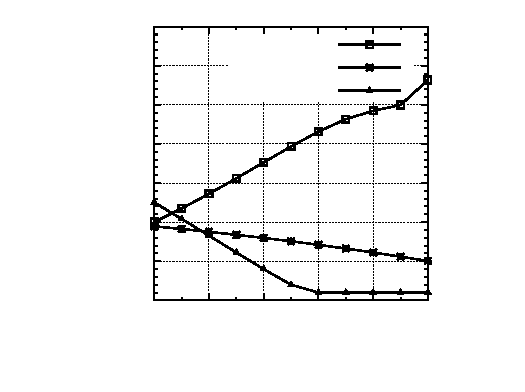
\includegraphics{figures/cnf-vol/cnf-vol}}%
    \gplfronttext
  \end{picture}%
\endgroup
\hspace*{-1.3cm}% GNUPLOT: LaTeX picture with Postscript
\begingroup
  \makeatletter
  \providecommand\color[2][]{%
    \GenericError{(gnuplot) \space\space\space\@spaces}{%
      Package color not loaded in conjunction with
      terminal option `colourtext'%
    }{See the gnuplot documentation for explanation.%
    }{Either use 'blacktext' in gnuplot or load the package
      color.sty in LaTeX.}%
    \renewcommand\color[2][]{}%
  }%
  \providecommand\includegraphics[2][]{%
    \GenericError{(gnuplot) \space\space\space\@spaces}{%
      Package graphicx or graphics not loaded%
    }{See the gnuplot documentation for explanation.%
    }{The gnuplot epslatex terminal needs graphicx.sty or graphics.sty.}%
    \renewcommand\includegraphics[2][]{}%
  }%
  \providecommand\rotatebox[2]{#2}%
  \@ifundefined{ifGPcolor}{%
    \newif\ifGPcolor
    \GPcolortrue
  }{}%
  \@ifundefined{ifGPblacktext}{%
    \newif\ifGPblacktext
    \GPblacktextfalse
  }{}%
  % define a \g@addto@macro without @ in the name:
  \let\gplgaddtomacro\g@addto@macro
  % define empty templates for all commands taking text:
  \gdef\gplbacktext{}%
  \gdef\gplfronttext{}%
  \makeatother
  \ifGPblacktext
    % no textcolor at all
    \def\colorrgb#1{}%
    \def\colorgray#1{}%
  \else
    % gray or color?
    \ifGPcolor
      \def\colorrgb#1{\color[rgb]{#1}}%
      \def\colorgray#1{\color[gray]{#1}}%
      \expandafter\def\csname LTw\endcsname{\color{white}}%
      \expandafter\def\csname LTb\endcsname{\color{black}}%
      \expandafter\def\csname LTa\endcsname{\color{black}}%
      \expandafter\def\csname LT0\endcsname{\color[rgb]{1,0,0}}%
      \expandafter\def\csname LT1\endcsname{\color[rgb]{0,1,0}}%
      \expandafter\def\csname LT2\endcsname{\color[rgb]{0,0,1}}%
      \expandafter\def\csname LT3\endcsname{\color[rgb]{1,0,1}}%
      \expandafter\def\csname LT4\endcsname{\color[rgb]{0,1,1}}%
      \expandafter\def\csname LT5\endcsname{\color[rgb]{1,1,0}}%
      \expandafter\def\csname LT6\endcsname{\color[rgb]{0,0,0}}%
      \expandafter\def\csname LT7\endcsname{\color[rgb]{1,0.3,0}}%
      \expandafter\def\csname LT8\endcsname{\color[rgb]{0.5,0.5,0.5}}%
    \else
      % gray
      \def\colorrgb#1{\color{black}}%
      \def\colorgray#1{\color[gray]{#1}}%
      \expandafter\def\csname LTw\endcsname{\color{white}}%
      \expandafter\def\csname LTb\endcsname{\color{black}}%
      \expandafter\def\csname LTa\endcsname{\color{black}}%
      \expandafter\def\csname LT0\endcsname{\color{black}}%
      \expandafter\def\csname LT1\endcsname{\color{black}}%
      \expandafter\def\csname LT2\endcsname{\color{black}}%
      \expandafter\def\csname LT3\endcsname{\color{black}}%
      \expandafter\def\csname LT4\endcsname{\color{black}}%
      \expandafter\def\csname LT5\endcsname{\color{black}}%
      \expandafter\def\csname LT6\endcsname{\color{black}}%
      \expandafter\def\csname LT7\endcsname{\color{black}}%
      \expandafter\def\csname LT8\endcsname{\color{black}}%
    \fi
  \fi
  \setlength{\unitlength}{0.0500bp}%
  \begin{picture}(5040.00,3772.00)%
    \gplgaddtomacro\gplbacktext{%
      \csname LTb\endcsname%
      \put(1415,880){\makebox(0,0)[r]{\strut{}-100}}%
      \csname LTb\endcsname%
      \put(1415,1284){\makebox(0,0)[r]{\strut{}-80}}%
      \csname LTb\endcsname%
      \put(1415,1688){\makebox(0,0)[r]{\strut{}-60}}%
      \csname LTb\endcsname%
      \put(1415,2092){\makebox(0,0)[r]{\strut{}-40}}%
      \csname LTb\endcsname%
      \put(1415,2497){\makebox(0,0)[r]{\strut{}-20}}%
      \csname LTb\endcsname%
      \put(1415,2901){\makebox(0,0)[r]{\strut{} 0}}%
      \csname LTb\endcsname%
      \put(1415,3305){\makebox(0,0)[r]{\strut{} 20}}%
      \csname LTb\endcsname%
      \put(1547,660){\makebox(0,0){\strut{} 0}}%
      \csname LTb\endcsname%
      \put(2072,660){\makebox(0,0){\strut{} 0.2}}%
      \csname LTb\endcsname%
      \put(2598,660){\makebox(0,0){\strut{} 0.4}}%
      \csname LTb\endcsname%
      \put(3123,660){\makebox(0,0){\strut{} 0.6}}%
      \csname LTb\endcsname%
      \put(3649,660){\makebox(0,0){\strut{} 0.8}}%
      \csname LTb\endcsname%
      \put(4174,660){\makebox(0,0){\strut{} 1}}%
      \put(645,2193){\rotatebox{-270}{\makebox(0,0){\strut{}$G^\prime_{\textrm{pol},i}$}}}%
      \put(2860,330){\makebox(0,0){\strut{}$\lambda$}}%
    }%
    \gplgaddtomacro\gplfronttext{%
      \csname LTb\endcsname%
      \put(3187,3334){\makebox(0,0)[r]{\strut{}C $\rightarrow$ F}}%
      \csname LTb\endcsname%
      \put(3187,3114){\makebox(0,0)[r]{\strut{}C}}%
      \csname LTb\endcsname%
      \put(3187,2894){\makebox(0,0)[r]{\strut{}N $\rightarrow$ Dummy}}%
    }%
    \gplbacktext
    \put(0,0){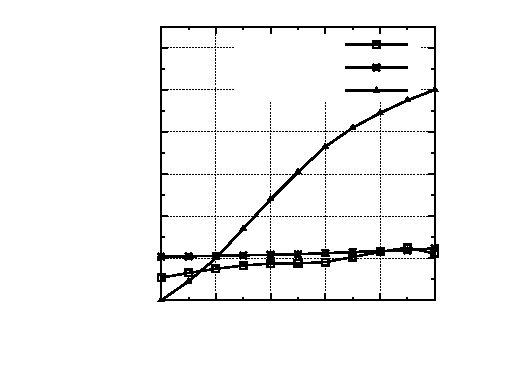
\includegraphics{figures/cnf-pol/cnf-pol}}%
    \gplfronttext
  \end{picture}%
\endgroup

\caption{The Born energy and components thereof for the perturbation of cyanobenzene to fluorobenzene. Top left: energy trajectory; top right: charge trajectories; bottom left: volume trajectories; bottom right: electrostatic trajectories.}
\label{cnf}
\end{figure}

PhCN $\longrightarrow$ PhF. Results for the perturbation of cyanobenzene to fluorobenzene are given in \cref{cnf}. Key atoms were determined to be the nitrogen being perturbed to a dummy atom, the carbon being perturbed to fluorine, and the carbon to which the carbon/fluorine was attached. Again, for all energies considered and components thereof, trajectories were smooth and consistent throughout the perturbation. This example was challenging as a test case due to the inclusion of a dummy atom, whose properties (or lack thereof) required special handling. Overall, the system was well behaved despite the challenges present. Of note were the trajectories of charge, volume, and electrostatic contribution for the nitrogen as it was perturbed to the dummy atom. Charge (\cref{cnf}, top right) was scaled linearly from $-0.43$ for nitrogen to zero for the dummy; atomic volume (\cref{cnf}, bottom left) was scaled linearly as well until a minimum of 1.0 \AA$^{3}$ was achieved at $\lambda = 0.6$. In this case, the minimum volume was reached before $\lambda = 1.0$ because of additional volume loss from overlap of the adjacent perturbation of carbon to fluorine, also reflected in the figure. Lastly, effective electrostatic contribution of the nitrogen was scaled smoothly, albeit not entirely linearly, to zero for the dummy. Other transformations were executed as anticipated, and the overall Born energy followed a smooth arch with a maximum change in energy at $\lambda = 0.8$ and an overall $\Delta G_{ \textrm{Born}}$ of $+3.2$ kcal/mol for the perturbation.

\begin{figure}[t!]
\centering
PhC(O)CH$_3$  $\longrightarrow$ PhC(O)NH$_2$\\
% GNUPLOT: LaTeX picture with Postscript
\begingroup
  \makeatletter
  \providecommand\color[2][]{%
    \GenericError{(gnuplot) \space\space\space\@spaces}{%
      Package color not loaded in conjunction with
      terminal option `colourtext'%
    }{See the gnuplot documentation for explanation.%
    }{Either use 'blacktext' in gnuplot or load the package
      color.sty in LaTeX.}%
    \renewcommand\color[2][]{}%
  }%
  \providecommand\includegraphics[2][]{%
    \GenericError{(gnuplot) \space\space\space\@spaces}{%
      Package graphicx or graphics not loaded%
    }{See the gnuplot documentation for explanation.%
    }{The gnuplot epslatex terminal needs graphicx.sty or graphics.sty.}%
    \renewcommand\includegraphics[2][]{}%
  }%
  \providecommand\rotatebox[2]{#2}%
  \@ifundefined{ifGPcolor}{%
    \newif\ifGPcolor
    \GPcolortrue
  }{}%
  \@ifundefined{ifGPblacktext}{%
    \newif\ifGPblacktext
    \GPblacktextfalse
  }{}%
  % define a \g@addto@macro without @ in the name:
  \let\gplgaddtomacro\g@addto@macro
  % define empty templates for all commands taking text:
  \gdef\gplbacktext{}%
  \gdef\gplfronttext{}%
  \makeatother
  \ifGPblacktext
    % no textcolor at all
    \def\colorrgb#1{}%
    \def\colorgray#1{}%
  \else
    % gray or color?
    \ifGPcolor
      \def\colorrgb#1{\color[rgb]{#1}}%
      \def\colorgray#1{\color[gray]{#1}}%
      \expandafter\def\csname LTw\endcsname{\color{white}}%
      \expandafter\def\csname LTb\endcsname{\color{black}}%
      \expandafter\def\csname LTa\endcsname{\color{black}}%
      \expandafter\def\csname LT0\endcsname{\color[rgb]{1,0,0}}%
      \expandafter\def\csname LT1\endcsname{\color[rgb]{0,1,0}}%
      \expandafter\def\csname LT2\endcsname{\color[rgb]{0,0,1}}%
      \expandafter\def\csname LT3\endcsname{\color[rgb]{1,0,1}}%
      \expandafter\def\csname LT4\endcsname{\color[rgb]{0,1,1}}%
      \expandafter\def\csname LT5\endcsname{\color[rgb]{1,1,0}}%
      \expandafter\def\csname LT6\endcsname{\color[rgb]{0,0,0}}%
      \expandafter\def\csname LT7\endcsname{\color[rgb]{1,0.3,0}}%
      \expandafter\def\csname LT8\endcsname{\color[rgb]{0.5,0.5,0.5}}%
    \else
      % gray
      \def\colorrgb#1{\color{black}}%
      \def\colorgray#1{\color[gray]{#1}}%
      \expandafter\def\csname LTw\endcsname{\color{white}}%
      \expandafter\def\csname LTb\endcsname{\color{black}}%
      \expandafter\def\csname LTa\endcsname{\color{black}}%
      \expandafter\def\csname LT0\endcsname{\color{black}}%
      \expandafter\def\csname LT1\endcsname{\color{black}}%
      \expandafter\def\csname LT2\endcsname{\color{black}}%
      \expandafter\def\csname LT3\endcsname{\color{black}}%
      \expandafter\def\csname LT4\endcsname{\color{black}}%
      \expandafter\def\csname LT5\endcsname{\color{black}}%
      \expandafter\def\csname LT6\endcsname{\color{black}}%
      \expandafter\def\csname LT7\endcsname{\color{black}}%
      \expandafter\def\csname LT8\endcsname{\color{black}}%
    \fi
  \fi
  \setlength{\unitlength}{0.0500bp}%
  \begin{picture}(5040.00,3772.00)%
    \gplgaddtomacro\gplbacktext{%
      \csname LTb\endcsname%
      \put(1349,880){\makebox(0,0)[r]{\strut{}-16}}%
      \csname LTb\endcsname%
      \put(1349,1358){\makebox(0,0)[r]{\strut{}-14}}%
      \csname LTb\endcsname%
      \put(1349,1835){\makebox(0,0)[r]{\strut{}-12}}%
      \csname LTb\endcsname%
      \put(1349,2313){\makebox(0,0)[r]{\strut{}-10}}%
      \csname LTb\endcsname%
      \put(1349,2791){\makebox(0,0)[r]{\strut{}-8}}%
      \csname LTb\endcsname%
      \put(1349,3268){\makebox(0,0)[r]{\strut{}-6}}%
      \csname LTb\endcsname%
      \put(1481,660){\makebox(0,0){\strut{} 0}}%
      \csname LTb\endcsname%
      \put(2006,660){\makebox(0,0){\strut{} 0.2}}%
      \csname LTb\endcsname%
      \put(2532,660){\makebox(0,0){\strut{} 0.4}}%
      \csname LTb\endcsname%
      \put(3057,660){\makebox(0,0){\strut{} 0.6}}%
      \csname LTb\endcsname%
      \put(3583,660){\makebox(0,0){\strut{} 0.8}}%
      \csname LTb\endcsname%
      \put(4108,660){\makebox(0,0){\strut{} 1}}%
      \csname LTb\endcsname%
      \put(711,2193){\rotatebox{-270}{\makebox(0,0){\strut{}Born energy (kcal/mol)}}}%
      \put(2794,330){\makebox(0,0){\strut{}$\lambda$}}%
    }%
    \gplgaddtomacro\gplfronttext{%
    }%
    \gplbacktext
    \put(0,0){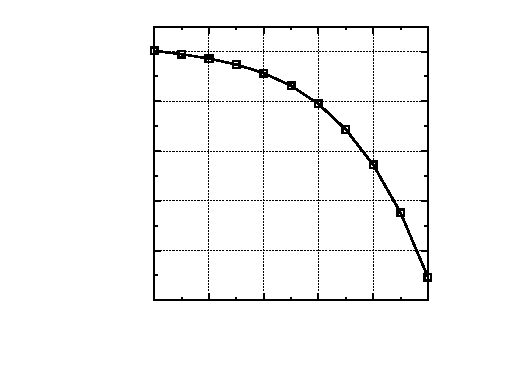
\includegraphics{figures/comenh2-en/comenh2-en}}%
    \gplfronttext
  \end{picture}%
\endgroup
\hspace*{-1.3cm}% GNUPLOT: LaTeX picture with Postscript
\begingroup
  \makeatletter
  \providecommand\color[2][]{%
    \GenericError{(gnuplot) \space\space\space\@spaces}{%
      Package color not loaded in conjunction with
      terminal option `colourtext'%
    }{See the gnuplot documentation for explanation.%
    }{Either use 'blacktext' in gnuplot or load the package
      color.sty in LaTeX.}%
    \renewcommand\color[2][]{}%
  }%
  \providecommand\includegraphics[2][]{%
    \GenericError{(gnuplot) \space\space\space\@spaces}{%
      Package graphicx or graphics not loaded%
    }{See the gnuplot documentation for explanation.%
    }{The gnuplot epslatex terminal needs graphicx.sty or graphics.sty.}%
    \renewcommand\includegraphics[2][]{}%
  }%
  \providecommand\rotatebox[2]{#2}%
  \@ifundefined{ifGPcolor}{%
    \newif\ifGPcolor
    \GPcolortrue
  }{}%
  \@ifundefined{ifGPblacktext}{%
    \newif\ifGPblacktext
    \GPblacktextfalse
  }{}%
  % define a \g@addto@macro without @ in the name:
  \let\gplgaddtomacro\g@addto@macro
  % define empty templates for all commands taking text:
  \gdef\gplbacktext{}%
  \gdef\gplfronttext{}%
  \makeatother
  \ifGPblacktext
    % no textcolor at all
    \def\colorrgb#1{}%
    \def\colorgray#1{}%
  \else
    % gray or color?
    \ifGPcolor
      \def\colorrgb#1{\color[rgb]{#1}}%
      \def\colorgray#1{\color[gray]{#1}}%
      \expandafter\def\csname LTw\endcsname{\color{white}}%
      \expandafter\def\csname LTb\endcsname{\color{black}}%
      \expandafter\def\csname LTa\endcsname{\color{black}}%
      \expandafter\def\csname LT0\endcsname{\color[rgb]{1,0,0}}%
      \expandafter\def\csname LT1\endcsname{\color[rgb]{0,1,0}}%
      \expandafter\def\csname LT2\endcsname{\color[rgb]{0,0,1}}%
      \expandafter\def\csname LT3\endcsname{\color[rgb]{1,0,1}}%
      \expandafter\def\csname LT4\endcsname{\color[rgb]{0,1,1}}%
      \expandafter\def\csname LT5\endcsname{\color[rgb]{1,1,0}}%
      \expandafter\def\csname LT6\endcsname{\color[rgb]{0,0,0}}%
      \expandafter\def\csname LT7\endcsname{\color[rgb]{1,0.3,0}}%
      \expandafter\def\csname LT8\endcsname{\color[rgb]{0.5,0.5,0.5}}%
    \else
      % gray
      \def\colorrgb#1{\color{black}}%
      \def\colorgray#1{\color[gray]{#1}}%
      \expandafter\def\csname LTw\endcsname{\color{white}}%
      \expandafter\def\csname LTb\endcsname{\color{black}}%
      \expandafter\def\csname LTa\endcsname{\color{black}}%
      \expandafter\def\csname LT0\endcsname{\color{black}}%
      \expandafter\def\csname LT1\endcsname{\color{black}}%
      \expandafter\def\csname LT2\endcsname{\color{black}}%
      \expandafter\def\csname LT3\endcsname{\color{black}}%
      \expandafter\def\csname LT4\endcsname{\color{black}}%
      \expandafter\def\csname LT5\endcsname{\color{black}}%
      \expandafter\def\csname LT6\endcsname{\color{black}}%
      \expandafter\def\csname LT7\endcsname{\color{black}}%
      \expandafter\def\csname LT8\endcsname{\color{black}}%
    \fi
  \fi
  \setlength{\unitlength}{0.0500bp}%
  \begin{picture}(5040.00,3772.00)%
    \gplgaddtomacro\gplbacktext{%
      \csname LTb\endcsname%
      \put(1415,880){\makebox(0,0)[r]{\strut{}-0.8}}%
      \csname LTb\endcsname%
      \put(1415,1208){\makebox(0,0)[r]{\strut{}-0.6}}%
      \csname LTb\endcsname%
      \put(1415,1537){\makebox(0,0)[r]{\strut{}-0.4}}%
      \csname LTb\endcsname%
      \put(1415,1865){\makebox(0,0)[r]{\strut{}-0.2}}%
      \csname LTb\endcsname%
      \put(1415,2194){\makebox(0,0)[r]{\strut{} 0}}%
      \csname LTb\endcsname%
      \put(1415,2522){\makebox(0,0)[r]{\strut{} 0.2}}%
      \csname LTb\endcsname%
      \put(1415,2850){\makebox(0,0)[r]{\strut{} 0.4}}%
      \csname LTb\endcsname%
      \put(1415,3179){\makebox(0,0)[r]{\strut{} 0.6}}%
      \csname LTb\endcsname%
      \put(1415,3507){\makebox(0,0)[r]{\strut{} 0.8}}%
      \csname LTb\endcsname%
      \put(1547,660){\makebox(0,0){\strut{} 0}}%
      \csname LTb\endcsname%
      \put(2072,660){\makebox(0,0){\strut{} 0.2}}%
      \csname LTb\endcsname%
      \put(2598,660){\makebox(0,0){\strut{} 0.4}}%
      \csname LTb\endcsname%
      \put(3123,660){\makebox(0,0){\strut{} 0.6}}%
      \csname LTb\endcsname%
      \put(3649,660){\makebox(0,0){\strut{} 0.8}}%
      \csname LTb\endcsname%
      \put(4174,660){\makebox(0,0){\strut{} 1}}%
      \put(645,2193){\rotatebox{-270}{\makebox(0,0){\strut{}charge}}}%
      \put(2860,330){\makebox(0,0){\strut{}$\lambda$}}%
    }%
    \gplgaddtomacro\gplfronttext{%
      \csname LTb\endcsname%
      \put(3187,3334){\makebox(0,0)[r]{\strut{}HC $\rightarrow$ HN}}%
      \csname LTb\endcsname%
      \put(3187,3114){\makebox(0,0)[r]{\strut{}C $\rightarrow$ N}}%
      \csname LTb\endcsname%
      \put(3187,2894){\makebox(0,0)[r]{\strut{}HC $\rightarrow$ Dummy}}%
    }%
    \gplbacktext
    \put(0,0){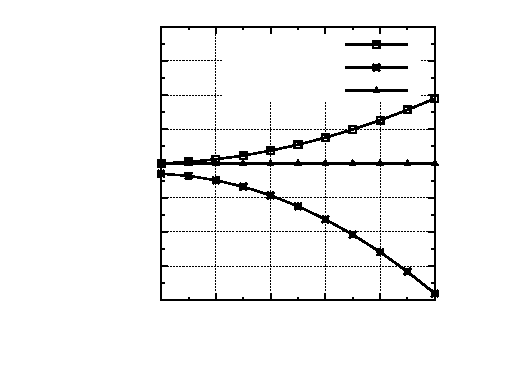
\includegraphics{figures/comenh2-charge/comenh2-charge}}%
    \gplfronttext
  \end{picture}%
\endgroup
\\
% GNUPLOT: LaTeX picture with Postscript
\begingroup
  \makeatletter
  \providecommand\color[2][]{%
    \GenericError{(gnuplot) \space\space\space\@spaces}{%
      Package color not loaded in conjunction with
      terminal option `colourtext'%
    }{See the gnuplot documentation for explanation.%
    }{Either use 'blacktext' in gnuplot or load the package
      color.sty in LaTeX.}%
    \renewcommand\color[2][]{}%
  }%
  \providecommand\includegraphics[2][]{%
    \GenericError{(gnuplot) \space\space\space\@spaces}{%
      Package graphicx or graphics not loaded%
    }{See the gnuplot documentation for explanation.%
    }{The gnuplot epslatex terminal needs graphicx.sty or graphics.sty.}%
    \renewcommand\includegraphics[2][]{}%
  }%
  \providecommand\rotatebox[2]{#2}%
  \@ifundefined{ifGPcolor}{%
    \newif\ifGPcolor
    \GPcolortrue
  }{}%
  \@ifundefined{ifGPblacktext}{%
    \newif\ifGPblacktext
    \GPblacktextfalse
  }{}%
  % define a \g@addto@macro without @ in the name:
  \let\gplgaddtomacro\g@addto@macro
  % define empty templates for all commands taking text:
  \gdef\gplbacktext{}%
  \gdef\gplfronttext{}%
  \makeatother
  \ifGPblacktext
    % no textcolor at all
    \def\colorrgb#1{}%
    \def\colorgray#1{}%
  \else
    % gray or color?
    \ifGPcolor
      \def\colorrgb#1{\color[rgb]{#1}}%
      \def\colorgray#1{\color[gray]{#1}}%
      \expandafter\def\csname LTw\endcsname{\color{white}}%
      \expandafter\def\csname LTb\endcsname{\color{black}}%
      \expandafter\def\csname LTa\endcsname{\color{black}}%
      \expandafter\def\csname LT0\endcsname{\color[rgb]{1,0,0}}%
      \expandafter\def\csname LT1\endcsname{\color[rgb]{0,1,0}}%
      \expandafter\def\csname LT2\endcsname{\color[rgb]{0,0,1}}%
      \expandafter\def\csname LT3\endcsname{\color[rgb]{1,0,1}}%
      \expandafter\def\csname LT4\endcsname{\color[rgb]{0,1,1}}%
      \expandafter\def\csname LT5\endcsname{\color[rgb]{1,1,0}}%
      \expandafter\def\csname LT6\endcsname{\color[rgb]{0,0,0}}%
      \expandafter\def\csname LT7\endcsname{\color[rgb]{1,0.3,0}}%
      \expandafter\def\csname LT8\endcsname{\color[rgb]{0.5,0.5,0.5}}%
    \else
      % gray
      \def\colorrgb#1{\color{black}}%
      \def\colorgray#1{\color[gray]{#1}}%
      \expandafter\def\csname LTw\endcsname{\color{white}}%
      \expandafter\def\csname LTb\endcsname{\color{black}}%
      \expandafter\def\csname LTa\endcsname{\color{black}}%
      \expandafter\def\csname LT0\endcsname{\color{black}}%
      \expandafter\def\csname LT1\endcsname{\color{black}}%
      \expandafter\def\csname LT2\endcsname{\color{black}}%
      \expandafter\def\csname LT3\endcsname{\color{black}}%
      \expandafter\def\csname LT4\endcsname{\color{black}}%
      \expandafter\def\csname LT5\endcsname{\color{black}}%
      \expandafter\def\csname LT6\endcsname{\color{black}}%
      \expandafter\def\csname LT7\endcsname{\color{black}}%
      \expandafter\def\csname LT8\endcsname{\color{black}}%
    \fi
  \fi
  \setlength{\unitlength}{0.0500bp}%
  \begin{picture}(5040.00,3772.00)%
    \gplgaddtomacro\gplbacktext{%
      \csname LTb\endcsname%
      \put(1349,880){\makebox(0,0)[r]{\strut{} 0}}%
      \csname LTb\endcsname%
      \put(1349,1172){\makebox(0,0)[r]{\strut{} 2}}%
      \csname LTb\endcsname%
      \put(1349,1464){\makebox(0,0)[r]{\strut{} 4}}%
      \csname LTb\endcsname%
      \put(1349,1756){\makebox(0,0)[r]{\strut{} 6}}%
      \csname LTb\endcsname%
      \put(1349,2048){\makebox(0,0)[r]{\strut{} 8}}%
      \csname LTb\endcsname%
      \put(1349,2339){\makebox(0,0)[r]{\strut{} 10}}%
      \csname LTb\endcsname%
      \put(1349,2631){\makebox(0,0)[r]{\strut{} 12}}%
      \csname LTb\endcsname%
      \put(1349,2923){\makebox(0,0)[r]{\strut{} 14}}%
      \csname LTb\endcsname%
      \put(1349,3215){\makebox(0,0)[r]{\strut{} 16}}%
      \csname LTb\endcsname%
      \put(1349,3507){\makebox(0,0)[r]{\strut{} 18}}%
      \csname LTb\endcsname%
      \put(1481,660){\makebox(0,0){\strut{} 0}}%
      \csname LTb\endcsname%
      \put(2006,660){\makebox(0,0){\strut{} 0.2}}%
      \csname LTb\endcsname%
      \put(2532,660){\makebox(0,0){\strut{} 0.4}}%
      \csname LTb\endcsname%
      \put(3057,660){\makebox(0,0){\strut{} 0.6}}%
      \csname LTb\endcsname%
      \put(3583,660){\makebox(0,0){\strut{} 0.8}}%
      \csname LTb\endcsname%
      \put(4108,660){\makebox(0,0){\strut{} 1}}%
      \put(711,2193){\rotatebox{-270}{\makebox(0,0){\strut{}volume (\AA$^{3}$)}}}%
      \put(2794,330){\makebox(0,0){\strut{}$\lambda$}}%
    }%
    \gplgaddtomacro\gplfronttext{%
      \csname LTb\endcsname%
      \put(3121,3334){\makebox(0,0)[r]{\strut{}HC $\rightarrow$ HN}}%
      \csname LTb\endcsname%
      \put(3121,3114){\makebox(0,0)[r]{\strut{}C $\rightarrow$ N}}%
      \csname LTb\endcsname%
      \put(3121,2894){\makebox(0,0)[r]{\strut{}HC $\rightarrow$ Dummy}}%
    }%
    \gplbacktext
    \put(0,0){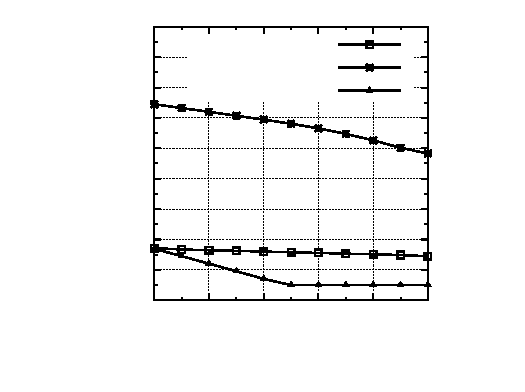
\includegraphics{figures/comenh2-vol/comenh2-vol}}%
    \gplfronttext
  \end{picture}%
\endgroup
\hspace*{-1.3cm}% GNUPLOT: LaTeX picture with Postscript
\begingroup
  \makeatletter
  \providecommand\color[2][]{%
    \GenericError{(gnuplot) \space\space\space\@spaces}{%
      Package color not loaded in conjunction with
      terminal option `colourtext'%
    }{See the gnuplot documentation for explanation.%
    }{Either use 'blacktext' in gnuplot or load the package
      color.sty in LaTeX.}%
    \renewcommand\color[2][]{}%
  }%
  \providecommand\includegraphics[2][]{%
    \GenericError{(gnuplot) \space\space\space\@spaces}{%
      Package graphicx or graphics not loaded%
    }{See the gnuplot documentation for explanation.%
    }{The gnuplot epslatex terminal needs graphicx.sty or graphics.sty.}%
    \renewcommand\includegraphics[2][]{}%
  }%
  \providecommand\rotatebox[2]{#2}%
  \@ifundefined{ifGPcolor}{%
    \newif\ifGPcolor
    \GPcolortrue
  }{}%
  \@ifundefined{ifGPblacktext}{%
    \newif\ifGPblacktext
    \GPblacktextfalse
  }{}%
  % define a \g@addto@macro without @ in the name:
  \let\gplgaddtomacro\g@addto@macro
  % define empty templates for all commands taking text:
  \gdef\gplbacktext{}%
  \gdef\gplfronttext{}%
  \makeatother
  \ifGPblacktext
    % no textcolor at all
    \def\colorrgb#1{}%
    \def\colorgray#1{}%
  \else
    % gray or color?
    \ifGPcolor
      \def\colorrgb#1{\color[rgb]{#1}}%
      \def\colorgray#1{\color[gray]{#1}}%
      \expandafter\def\csname LTw\endcsname{\color{white}}%
      \expandafter\def\csname LTb\endcsname{\color{black}}%
      \expandafter\def\csname LTa\endcsname{\color{black}}%
      \expandafter\def\csname LT0\endcsname{\color[rgb]{1,0,0}}%
      \expandafter\def\csname LT1\endcsname{\color[rgb]{0,1,0}}%
      \expandafter\def\csname LT2\endcsname{\color[rgb]{0,0,1}}%
      \expandafter\def\csname LT3\endcsname{\color[rgb]{1,0,1}}%
      \expandafter\def\csname LT4\endcsname{\color[rgb]{0,1,1}}%
      \expandafter\def\csname LT5\endcsname{\color[rgb]{1,1,0}}%
      \expandafter\def\csname LT6\endcsname{\color[rgb]{0,0,0}}%
      \expandafter\def\csname LT7\endcsname{\color[rgb]{1,0.3,0}}%
      \expandafter\def\csname LT8\endcsname{\color[rgb]{0.5,0.5,0.5}}%
    \else
      % gray
      \def\colorrgb#1{\color{black}}%
      \def\colorgray#1{\color[gray]{#1}}%
      \expandafter\def\csname LTw\endcsname{\color{white}}%
      \expandafter\def\csname LTb\endcsname{\color{black}}%
      \expandafter\def\csname LTa\endcsname{\color{black}}%
      \expandafter\def\csname LT0\endcsname{\color{black}}%
      \expandafter\def\csname LT1\endcsname{\color{black}}%
      \expandafter\def\csname LT2\endcsname{\color{black}}%
      \expandafter\def\csname LT3\endcsname{\color{black}}%
      \expandafter\def\csname LT4\endcsname{\color{black}}%
      \expandafter\def\csname LT5\endcsname{\color{black}}%
      \expandafter\def\csname LT6\endcsname{\color{black}}%
      \expandafter\def\csname LT7\endcsname{\color{black}}%
      \expandafter\def\csname LT8\endcsname{\color{black}}%
    \fi
  \fi
  \setlength{\unitlength}{0.0500bp}%
  \begin{picture}(5040.00,3772.00)%
    \gplgaddtomacro\gplbacktext{%
      \csname LTb\endcsname%
      \put(1415,1405){\makebox(0,0)[r]{\strut{}-100}}%
      \csname LTb\endcsname%
      \put(1415,2062){\makebox(0,0)[r]{\strut{}-50}}%
      \csname LTb\endcsname%
      \put(1415,2719){\makebox(0,0)[r]{\strut{} 0}}%
      \csname LTb\endcsname%
      \put(1415,3376){\makebox(0,0)[r]{\strut{} 50}}%
      \csname LTb\endcsname%
      \put(1547,660){\makebox(0,0){\strut{} 0}}%
      \csname LTb\endcsname%
      \put(2072,660){\makebox(0,0){\strut{} 0.2}}%
      \csname LTb\endcsname%
      \put(2598,660){\makebox(0,0){\strut{} 0.4}}%
      \csname LTb\endcsname%
      \put(3123,660){\makebox(0,0){\strut{} 0.6}}%
      \csname LTb\endcsname%
      \put(3649,660){\makebox(0,0){\strut{} 0.8}}%
      \csname LTb\endcsname%
      \put(4174,660){\makebox(0,0){\strut{} 1}}%
      \put(645,2193){\rotatebox{-270}{\makebox(0,0){\strut{}$G^\prime_{\textrm{pol},i}$}}}%
      \put(2860,330){\makebox(0,0){\strut{}$\lambda$}}%
    }%
    \gplgaddtomacro\gplfronttext{%
      \csname LTb\endcsname%
      \put(3187,3334){\makebox(0,0)[r]{\strut{}HC $\rightarrow$ HN}}%
      \csname LTb\endcsname%
      \put(3187,3114){\makebox(0,0)[r]{\strut{}C $\rightarrow$ N}}%
      \csname LTb\endcsname%
      \put(3187,2894){\makebox(0,0)[r]{\strut{}HC $\rightarrow$ Dummy}}%
    }%
    \gplbacktext
    \put(0,0){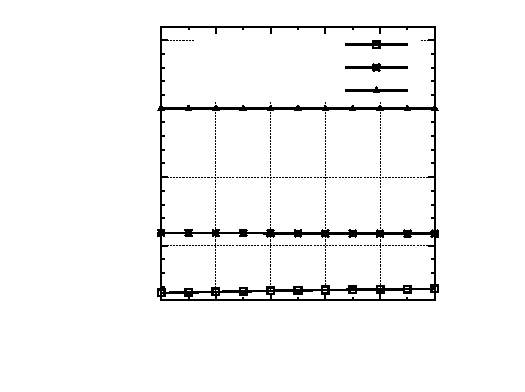
\includegraphics{figures/comenh2-pol/comenh2-pol}}%
    \gplfronttext
  \end{picture}%
\endgroup

\caption{The Born energy and components thereof for the perturbation of acetophenone to benzamide. Top left: energy trajectory; top right: charge trajectories; bottom left: volume trajectories; bottom right: electrostatic trajectories.}
\label{comenh2}
\end{figure}

PhC(O)CH$_3$  $\longrightarrow$ PhC(O)NH$_2$. Results for the perturbation of acetophenone to benzamide are given in \cref{comenh2}. This test case was particularly complicated, featuring three perturbations (hydrogen on carbon to hydrogen on nitrogen, carbon to nitrogen, and hydrogen to dummy), which included a dummy atom as well as a geometry change (methyl to amino). Further complicating the energetics was the methyl contribution to the electrostatic energy; recall that for H--C neighboring pairs where C is fully saturated, 1,2 and 1,3 contribution to the electrostatic energy is ignored. Thus, in this case, such contribution to the electrostatic energy is ignored for the methyl group in acetophenone but not for the amido group in benzamide. Gratifyingly, for all energies considered and components thereof, trajectories were smooth and consistent throughout the perturbation and trends played out as was anticipated. For atomic charges (\cref{comenh2}, top right), a significant change in charge was observed for methyl carbon to amido nitrogen. Of note was the observed change in charge for hydrogen on carbon to hydrogen on nitrogen. Recall that hydrogens on saturated carbons are treated in a united-atom fashion such that their charges are condensed onto the neighboring carbon. Contrarily, hydrogens on heteroatoms are treated in an all-atom fashion. Thus, charges on the methyl hydrogens were expanded throughout the simulation, from zero at $\lambda = 0$ to $+7.5$ at $\lambda = 1.0$. However, for one methyl hydrogen this was not the case; the condensed-charge methyl hydrogen that was perturbed to a dummy atom maintained its zero charge throughout the perturbation. Schematically, the charge trajectories give a visual depiction to the overall charge dispersion for the perturbation of acetophenone to benzamide. Like in the perturbation of cyanobenzene to fluorobenzene, the hydrogen to dummy perturbation reached a minimum volume of 1.0 \AA$^{3}$ near the midpoint of $\lambda$ (\cref{comenh2}, bottom left) and the effective contribution to the electrostatic polarization of the methyl hydrogen to dummy was held at zero. Other transformations were unremarkable, yielding a smooth overall Born energy trajectory and $\Delta G_{ \textrm{Born}}$ of $-9.2$ kcal/mol for the perturbation.


\begin{figure}[t!]
\centering
PhPr $\longrightarrow$ BzOCH$_3$\\
% GNUPLOT: LaTeX picture with Postscript
\begingroup
  \makeatletter
  \providecommand\color[2][]{%
    \GenericError{(gnuplot) \space\space\space\@spaces}{%
      Package color not loaded in conjunction with
      terminal option `colourtext'%
    }{See the gnuplot documentation for explanation.%
    }{Either use 'blacktext' in gnuplot or load the package
      color.sty in LaTeX.}%
    \renewcommand\color[2][]{}%
  }%
  \providecommand\includegraphics[2][]{%
    \GenericError{(gnuplot) \space\space\space\@spaces}{%
      Package graphicx or graphics not loaded%
    }{See the gnuplot documentation for explanation.%
    }{The gnuplot epslatex terminal needs graphicx.sty or graphics.sty.}%
    \renewcommand\includegraphics[2][]{}%
  }%
  \providecommand\rotatebox[2]{#2}%
  \@ifundefined{ifGPcolor}{%
    \newif\ifGPcolor
    \GPcolortrue
  }{}%
  \@ifundefined{ifGPblacktext}{%
    \newif\ifGPblacktext
    \GPblacktextfalse
  }{}%
  % define a \g@addto@macro without @ in the name:
  \let\gplgaddtomacro\g@addto@macro
  % define empty templates for all commands taking text:
  \gdef\gplbacktext{}%
  \gdef\gplfronttext{}%
  \makeatother
  \ifGPblacktext
    % no textcolor at all
    \def\colorrgb#1{}%
    \def\colorgray#1{}%
  \else
    % gray or color?
    \ifGPcolor
      \def\colorrgb#1{\color[rgb]{#1}}%
      \def\colorgray#1{\color[gray]{#1}}%
      \expandafter\def\csname LTw\endcsname{\color{white}}%
      \expandafter\def\csname LTb\endcsname{\color{black}}%
      \expandafter\def\csname LTa\endcsname{\color{black}}%
      \expandafter\def\csname LT0\endcsname{\color[rgb]{1,0,0}}%
      \expandafter\def\csname LT1\endcsname{\color[rgb]{0,1,0}}%
      \expandafter\def\csname LT2\endcsname{\color[rgb]{0,0,1}}%
      \expandafter\def\csname LT3\endcsname{\color[rgb]{1,0,1}}%
      \expandafter\def\csname LT4\endcsname{\color[rgb]{0,1,1}}%
      \expandafter\def\csname LT5\endcsname{\color[rgb]{1,1,0}}%
      \expandafter\def\csname LT6\endcsname{\color[rgb]{0,0,0}}%
      \expandafter\def\csname LT7\endcsname{\color[rgb]{1,0.3,0}}%
      \expandafter\def\csname LT8\endcsname{\color[rgb]{0.5,0.5,0.5}}%
    \else
      % gray
      \def\colorrgb#1{\color{black}}%
      \def\colorgray#1{\color[gray]{#1}}%
      \expandafter\def\csname LTw\endcsname{\color{white}}%
      \expandafter\def\csname LTb\endcsname{\color{black}}%
      \expandafter\def\csname LTa\endcsname{\color{black}}%
      \expandafter\def\csname LT0\endcsname{\color{black}}%
      \expandafter\def\csname LT1\endcsname{\color{black}}%
      \expandafter\def\csname LT2\endcsname{\color{black}}%
      \expandafter\def\csname LT3\endcsname{\color{black}}%
      \expandafter\def\csname LT4\endcsname{\color{black}}%
      \expandafter\def\csname LT5\endcsname{\color{black}}%
      \expandafter\def\csname LT6\endcsname{\color{black}}%
      \expandafter\def\csname LT7\endcsname{\color{black}}%
      \expandafter\def\csname LT8\endcsname{\color{black}}%
    \fi
  \fi
  \setlength{\unitlength}{0.0500bp}%
  \begin{picture}(5040.00,3772.00)%
    \gplgaddtomacro\gplbacktext{%
      \csname LTb\endcsname%
      \put(1415,880){\makebox(0,0)[r]{\strut{}-5.5}}%
      \csname LTb\endcsname%
      \put(1415,1405){\makebox(0,0)[r]{\strut{}-5}}%
      \csname LTb\endcsname%
      \put(1415,1931){\makebox(0,0)[r]{\strut{}-4.5}}%
      \csname LTb\endcsname%
      \put(1415,2456){\makebox(0,0)[r]{\strut{}-4}}%
      \csname LTb\endcsname%
      \put(1415,2982){\makebox(0,0)[r]{\strut{}-3.5}}%
      \csname LTb\endcsname%
      \put(1415,3507){\makebox(0,0)[r]{\strut{}-3}}%
      \csname LTb\endcsname%
      \put(1547,660){\makebox(0,0){\strut{} 0}}%
      \csname LTb\endcsname%
      \put(2072,660){\makebox(0,0){\strut{} 0.2}}%
      \csname LTb\endcsname%
      \put(2598,660){\makebox(0,0){\strut{} 0.4}}%
      \csname LTb\endcsname%
      \put(3123,660){\makebox(0,0){\strut{} 0.6}}%
      \csname LTb\endcsname%
      \put(3649,660){\makebox(0,0){\strut{} 0.8}}%
      \csname LTb\endcsname%
      \put(4174,660){\makebox(0,0){\strut{} 1}}%
      \csname LTb\endcsname%
      \put(645,2193){\rotatebox{-270}{\makebox(0,0){\strut{}Born energy (kcal/mol)}}}%
      \put(2860,330){\makebox(0,0){\strut{}$\lambda$}}%
    }%
    \gplgaddtomacro\gplfronttext{%
    }%
    \gplbacktext
    \put(0,0){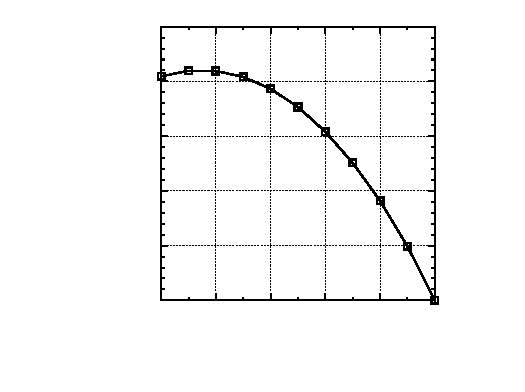
\includegraphics{figures/prmom-en/prmom-en}}%
    \gplfronttext
  \end{picture}%
\endgroup
\hspace*{-1.3cm}% GNUPLOT: LaTeX picture with Postscript
\begingroup
  \makeatletter
  \providecommand\color[2][]{%
    \GenericError{(gnuplot) \space\space\space\@spaces}{%
      Package color not loaded in conjunction with
      terminal option `colourtext'%
    }{See the gnuplot documentation for explanation.%
    }{Either use 'blacktext' in gnuplot or load the package
      color.sty in LaTeX.}%
    \renewcommand\color[2][]{}%
  }%
  \providecommand\includegraphics[2][]{%
    \GenericError{(gnuplot) \space\space\space\@spaces}{%
      Package graphicx or graphics not loaded%
    }{See the gnuplot documentation for explanation.%
    }{The gnuplot epslatex terminal needs graphicx.sty or graphics.sty.}%
    \renewcommand\includegraphics[2][]{}%
  }%
  \providecommand\rotatebox[2]{#2}%
  \@ifundefined{ifGPcolor}{%
    \newif\ifGPcolor
    \GPcolortrue
  }{}%
  \@ifundefined{ifGPblacktext}{%
    \newif\ifGPblacktext
    \GPblacktextfalse
  }{}%
  % define a \g@addto@macro without @ in the name:
  \let\gplgaddtomacro\g@addto@macro
  % define empty templates for all commands taking text:
  \gdef\gplbacktext{}%
  \gdef\gplfronttext{}%
  \makeatother
  \ifGPblacktext
    % no textcolor at all
    \def\colorrgb#1{}%
    \def\colorgray#1{}%
  \else
    % gray or color?
    \ifGPcolor
      \def\colorrgb#1{\color[rgb]{#1}}%
      \def\colorgray#1{\color[gray]{#1}}%
      \expandafter\def\csname LTw\endcsname{\color{white}}%
      \expandafter\def\csname LTb\endcsname{\color{black}}%
      \expandafter\def\csname LTa\endcsname{\color{black}}%
      \expandafter\def\csname LT0\endcsname{\color[rgb]{1,0,0}}%
      \expandafter\def\csname LT1\endcsname{\color[rgb]{0,1,0}}%
      \expandafter\def\csname LT2\endcsname{\color[rgb]{0,0,1}}%
      \expandafter\def\csname LT3\endcsname{\color[rgb]{1,0,1}}%
      \expandafter\def\csname LT4\endcsname{\color[rgb]{0,1,1}}%
      \expandafter\def\csname LT5\endcsname{\color[rgb]{1,1,0}}%
      \expandafter\def\csname LT6\endcsname{\color[rgb]{0,0,0}}%
      \expandafter\def\csname LT7\endcsname{\color[rgb]{1,0.3,0}}%
      \expandafter\def\csname LT8\endcsname{\color[rgb]{0.5,0.5,0.5}}%
    \else
      % gray
      \def\colorrgb#1{\color{black}}%
      \def\colorgray#1{\color[gray]{#1}}%
      \expandafter\def\csname LTw\endcsname{\color{white}}%
      \expandafter\def\csname LTb\endcsname{\color{black}}%
      \expandafter\def\csname LTa\endcsname{\color{black}}%
      \expandafter\def\csname LT0\endcsname{\color{black}}%
      \expandafter\def\csname LT1\endcsname{\color{black}}%
      \expandafter\def\csname LT2\endcsname{\color{black}}%
      \expandafter\def\csname LT3\endcsname{\color{black}}%
      \expandafter\def\csname LT4\endcsname{\color{black}}%
      \expandafter\def\csname LT5\endcsname{\color{black}}%
      \expandafter\def\csname LT6\endcsname{\color{black}}%
      \expandafter\def\csname LT7\endcsname{\color{black}}%
      \expandafter\def\csname LT8\endcsname{\color{black}}%
    \fi
  \fi
  \setlength{\unitlength}{0.0500bp}%
  \begin{picture}(5040.00,3772.00)%
    \gplgaddtomacro\gplbacktext{%
      \csname LTb\endcsname%
      \put(1415,1143){\makebox(0,0)[r]{\strut{}-0.4}}%
      \csname LTb\endcsname%
      \put(1415,1668){\makebox(0,0)[r]{\strut{}-0.2}}%
      \csname LTb\endcsname%
      \put(1415,2194){\makebox(0,0)[r]{\strut{} 0}}%
      \csname LTb\endcsname%
      \put(1415,2719){\makebox(0,0)[r]{\strut{} 0.2}}%
      \csname LTb\endcsname%
      \put(1415,3244){\makebox(0,0)[r]{\strut{} 0.4}}%
      \csname LTb\endcsname%
      \put(1547,660){\makebox(0,0){\strut{} 0}}%
      \csname LTb\endcsname%
      \put(2072,660){\makebox(0,0){\strut{} 0.2}}%
      \csname LTb\endcsname%
      \put(2598,660){\makebox(0,0){\strut{} 0.4}}%
      \csname LTb\endcsname%
      \put(3123,660){\makebox(0,0){\strut{} 0.6}}%
      \csname LTb\endcsname%
      \put(3649,660){\makebox(0,0){\strut{} 0.8}}%
      \csname LTb\endcsname%
      \put(4174,660){\makebox(0,0){\strut{} 1}}%
      \put(645,2193){\rotatebox{-270}{\makebox(0,0){\strut{}charge}}}%
      \put(2860,330){\makebox(0,0){\strut{}$\lambda$}}%
    }%
    \gplgaddtomacro\gplfronttext{%
      \csname LTb\endcsname%
      \put(3187,3334){\makebox(0,0)[r]{\strut{}C $\rightarrow$ O}}%
      \csname LTb\endcsname%
      \put(3187,3114){\makebox(0,0)[r]{\strut{}C}}%
      \csname LTb\endcsname%
      \put(3187,2894){\makebox(0,0)[r]{\strut{}H $\rightarrow$ Dummy}}%
    }%
    \gplbacktext
    \put(0,0){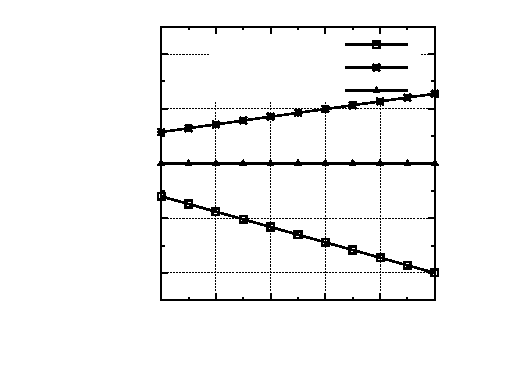
\includegraphics{figures/prmom-charge/prmom-charge}}%
    \gplfronttext
  \end{picture}%
\endgroup
\\
% GNUPLOT: LaTeX picture with Postscript
\begingroup
  \makeatletter
  \providecommand\color[2][]{%
    \GenericError{(gnuplot) \space\space\space\@spaces}{%
      Package color not loaded in conjunction with
      terminal option `colourtext'%
    }{See the gnuplot documentation for explanation.%
    }{Either use 'blacktext' in gnuplot or load the package
      color.sty in LaTeX.}%
    \renewcommand\color[2][]{}%
  }%
  \providecommand\includegraphics[2][]{%
    \GenericError{(gnuplot) \space\space\space\@spaces}{%
      Package graphicx or graphics not loaded%
    }{See the gnuplot documentation for explanation.%
    }{The gnuplot epslatex terminal needs graphicx.sty or graphics.sty.}%
    \renewcommand\includegraphics[2][]{}%
  }%
  \providecommand\rotatebox[2]{#2}%
  \@ifundefined{ifGPcolor}{%
    \newif\ifGPcolor
    \GPcolortrue
  }{}%
  \@ifundefined{ifGPblacktext}{%
    \newif\ifGPblacktext
    \GPblacktextfalse
  }{}%
  % define a \g@addto@macro without @ in the name:
  \let\gplgaddtomacro\g@addto@macro
  % define empty templates for all commands taking text:
  \gdef\gplbacktext{}%
  \gdef\gplfronttext{}%
  \makeatother
  \ifGPblacktext
    % no textcolor at all
    \def\colorrgb#1{}%
    \def\colorgray#1{}%
  \else
    % gray or color?
    \ifGPcolor
      \def\colorrgb#1{\color[rgb]{#1}}%
      \def\colorgray#1{\color[gray]{#1}}%
      \expandafter\def\csname LTw\endcsname{\color{white}}%
      \expandafter\def\csname LTb\endcsname{\color{black}}%
      \expandafter\def\csname LTa\endcsname{\color{black}}%
      \expandafter\def\csname LT0\endcsname{\color[rgb]{1,0,0}}%
      \expandafter\def\csname LT1\endcsname{\color[rgb]{0,1,0}}%
      \expandafter\def\csname LT2\endcsname{\color[rgb]{0,0,1}}%
      \expandafter\def\csname LT3\endcsname{\color[rgb]{1,0,1}}%
      \expandafter\def\csname LT4\endcsname{\color[rgb]{0,1,1}}%
      \expandafter\def\csname LT5\endcsname{\color[rgb]{1,1,0}}%
      \expandafter\def\csname LT6\endcsname{\color[rgb]{0,0,0}}%
      \expandafter\def\csname LT7\endcsname{\color[rgb]{1,0.3,0}}%
      \expandafter\def\csname LT8\endcsname{\color[rgb]{0.5,0.5,0.5}}%
    \else
      % gray
      \def\colorrgb#1{\color{black}}%
      \def\colorgray#1{\color[gray]{#1}}%
      \expandafter\def\csname LTw\endcsname{\color{white}}%
      \expandafter\def\csname LTb\endcsname{\color{black}}%
      \expandafter\def\csname LTa\endcsname{\color{black}}%
      \expandafter\def\csname LT0\endcsname{\color{black}}%
      \expandafter\def\csname LT1\endcsname{\color{black}}%
      \expandafter\def\csname LT2\endcsname{\color{black}}%
      \expandafter\def\csname LT3\endcsname{\color{black}}%
      \expandafter\def\csname LT4\endcsname{\color{black}}%
      \expandafter\def\csname LT5\endcsname{\color{black}}%
      \expandafter\def\csname LT6\endcsname{\color{black}}%
      \expandafter\def\csname LT7\endcsname{\color{black}}%
      \expandafter\def\csname LT8\endcsname{\color{black}}%
    \fi
  \fi
  \setlength{\unitlength}{0.0500bp}%
  \begin{picture}(5040.00,3772.00)%
    \gplgaddtomacro\gplbacktext{%
      \csname LTb\endcsname%
      \put(1349,880){\makebox(0,0)[r]{\strut{} 0}}%
      \csname LTb\endcsname%
      \put(1349,1172){\makebox(0,0)[r]{\strut{} 2}}%
      \csname LTb\endcsname%
      \put(1349,1464){\makebox(0,0)[r]{\strut{} 4}}%
      \csname LTb\endcsname%
      \put(1349,1756){\makebox(0,0)[r]{\strut{} 6}}%
      \csname LTb\endcsname%
      \put(1349,2048){\makebox(0,0)[r]{\strut{} 8}}%
      \csname LTb\endcsname%
      \put(1349,2339){\makebox(0,0)[r]{\strut{} 10}}%
      \csname LTb\endcsname%
      \put(1349,2631){\makebox(0,0)[r]{\strut{} 12}}%
      \csname LTb\endcsname%
      \put(1349,2923){\makebox(0,0)[r]{\strut{} 14}}%
      \csname LTb\endcsname%
      \put(1349,3215){\makebox(0,0)[r]{\strut{} 16}}%
      \csname LTb\endcsname%
      \put(1349,3507){\makebox(0,0)[r]{\strut{} 18}}%
      \csname LTb\endcsname%
      \put(1481,660){\makebox(0,0){\strut{} 0}}%
      \csname LTb\endcsname%
      \put(2006,660){\makebox(0,0){\strut{} 0.2}}%
      \csname LTb\endcsname%
      \put(2532,660){\makebox(0,0){\strut{} 0.4}}%
      \csname LTb\endcsname%
      \put(3057,660){\makebox(0,0){\strut{} 0.6}}%
      \csname LTb\endcsname%
      \put(3583,660){\makebox(0,0){\strut{} 0.8}}%
      \csname LTb\endcsname%
      \put(4108,660){\makebox(0,0){\strut{} 1}}%
      \put(711,2193){\rotatebox{-270}{\makebox(0,0){\strut{}volume (\AA$^{3}$)}}}%
      \put(2794,330){\makebox(0,0){\strut{}$\lambda$}}%
    }%
    \gplgaddtomacro\gplfronttext{%
      \csname LTb\endcsname%
      \put(3121,3334){\makebox(0,0)[r]{\strut{}C $\rightarrow$ O}}%
      \csname LTb\endcsname%
      \put(3121,3114){\makebox(0,0)[r]{\strut{}C}}%
      \csname LTb\endcsname%
      \put(3121,2894){\makebox(0,0)[r]{\strut{}H $\rightarrow$ Dummy}}%
    }%
    \gplbacktext
    \put(0,0){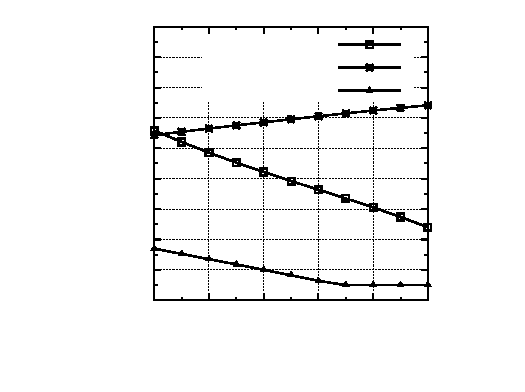
\includegraphics{figures/prmom-vol/prmom-vol}}%
    \gplfronttext
  \end{picture}%
\endgroup
\hspace*{-1.3cm}% GNUPLOT: LaTeX picture with Postscript
\begingroup
  \makeatletter
  \providecommand\color[2][]{%
    \GenericError{(gnuplot) \space\space\space\@spaces}{%
      Package color not loaded in conjunction with
      terminal option `colourtext'%
    }{See the gnuplot documentation for explanation.%
    }{Either use 'blacktext' in gnuplot or load the package
      color.sty in LaTeX.}%
    \renewcommand\color[2][]{}%
  }%
  \providecommand\includegraphics[2][]{%
    \GenericError{(gnuplot) \space\space\space\@spaces}{%
      Package graphicx or graphics not loaded%
    }{See the gnuplot documentation for explanation.%
    }{The gnuplot epslatex terminal needs graphicx.sty or graphics.sty.}%
    \renewcommand\includegraphics[2][]{}%
  }%
  \providecommand\rotatebox[2]{#2}%
  \@ifundefined{ifGPcolor}{%
    \newif\ifGPcolor
    \GPcolortrue
  }{}%
  \@ifundefined{ifGPblacktext}{%
    \newif\ifGPblacktext
    \GPblacktextfalse
  }{}%
  % define a \g@addto@macro without @ in the name:
  \let\gplgaddtomacro\g@addto@macro
  % define empty templates for all commands taking text:
  \gdef\gplbacktext{}%
  \gdef\gplfronttext{}%
  \makeatother
  \ifGPblacktext
    % no textcolor at all
    \def\colorrgb#1{}%
    \def\colorgray#1{}%
  \else
    % gray or color?
    \ifGPcolor
      \def\colorrgb#1{\color[rgb]{#1}}%
      \def\colorgray#1{\color[gray]{#1}}%
      \expandafter\def\csname LTw\endcsname{\color{white}}%
      \expandafter\def\csname LTb\endcsname{\color{black}}%
      \expandafter\def\csname LTa\endcsname{\color{black}}%
      \expandafter\def\csname LT0\endcsname{\color[rgb]{1,0,0}}%
      \expandafter\def\csname LT1\endcsname{\color[rgb]{0,1,0}}%
      \expandafter\def\csname LT2\endcsname{\color[rgb]{0,0,1}}%
      \expandafter\def\csname LT3\endcsname{\color[rgb]{1,0,1}}%
      \expandafter\def\csname LT4\endcsname{\color[rgb]{0,1,1}}%
      \expandafter\def\csname LT5\endcsname{\color[rgb]{1,1,0}}%
      \expandafter\def\csname LT6\endcsname{\color[rgb]{0,0,0}}%
      \expandafter\def\csname LT7\endcsname{\color[rgb]{1,0.3,0}}%
      \expandafter\def\csname LT8\endcsname{\color[rgb]{0.5,0.5,0.5}}%
    \else
      % gray
      \def\colorrgb#1{\color{black}}%
      \def\colorgray#1{\color[gray]{#1}}%
      \expandafter\def\csname LTw\endcsname{\color{white}}%
      \expandafter\def\csname LTb\endcsname{\color{black}}%
      \expandafter\def\csname LTa\endcsname{\color{black}}%
      \expandafter\def\csname LT0\endcsname{\color{black}}%
      \expandafter\def\csname LT1\endcsname{\color{black}}%
      \expandafter\def\csname LT2\endcsname{\color{black}}%
      \expandafter\def\csname LT3\endcsname{\color{black}}%
      \expandafter\def\csname LT4\endcsname{\color{black}}%
      \expandafter\def\csname LT5\endcsname{\color{black}}%
      \expandafter\def\csname LT6\endcsname{\color{black}}%
      \expandafter\def\csname LT7\endcsname{\color{black}}%
      \expandafter\def\csname LT8\endcsname{\color{black}}%
    \fi
  \fi
  \setlength{\unitlength}{0.0500bp}%
  \begin{picture}(5040.00,3772.00)%
    \gplgaddtomacro\gplbacktext{%
      \csname LTb\endcsname%
      \put(1415,1044){\makebox(0,0)[r]{\strut{}-100}}%
      \csname LTb\endcsname%
      \put(1415,1373){\makebox(0,0)[r]{\strut{}-80}}%
      \csname LTb\endcsname%
      \put(1415,1701){\makebox(0,0)[r]{\strut{}-60}}%
      \csname LTb\endcsname%
      \put(1415,2029){\makebox(0,0)[r]{\strut{}-40}}%
      \csname LTb\endcsname%
      \put(1415,2358){\makebox(0,0)[r]{\strut{}-20}}%
      \csname LTb\endcsname%
      \put(1415,2686){\makebox(0,0)[r]{\strut{} 0}}%
      \csname LTb\endcsname%
      \put(1415,3014){\makebox(0,0)[r]{\strut{} 20}}%
      \csname LTb\endcsname%
      \put(1415,3343){\makebox(0,0)[r]{\strut{} 40}}%
      \csname LTb\endcsname%
      \put(1547,660){\makebox(0,0){\strut{} 0}}%
      \csname LTb\endcsname%
      \put(2072,660){\makebox(0,0){\strut{} 0.2}}%
      \csname LTb\endcsname%
      \put(2598,660){\makebox(0,0){\strut{} 0.4}}%
      \csname LTb\endcsname%
      \put(3123,660){\makebox(0,0){\strut{} 0.6}}%
      \csname LTb\endcsname%
      \put(3649,660){\makebox(0,0){\strut{} 0.8}}%
      \csname LTb\endcsname%
      \put(4174,660){\makebox(0,0){\strut{} 1}}%
      \put(645,2193){\rotatebox{-270}{\makebox(0,0){\strut{}$G^\prime_{\textrm{pol},i}$}}}%
      \put(2860,330){\makebox(0,0){\strut{}$\lambda$}}%
    }%
    \gplgaddtomacro\gplfronttext{%
      \csname LTb\endcsname%
      \put(3187,3334){\makebox(0,0)[r]{\strut{}C $\rightarrow$ O}}%
      \csname LTb\endcsname%
      \put(3187,3114){\makebox(0,0)[r]{\strut{}C}}%
      \csname LTb\endcsname%
      \put(3187,2894){\makebox(0,0)[r]{\strut{}H $\rightarrow$ Dummy}}%
    }%
    \gplbacktext
    \put(0,0){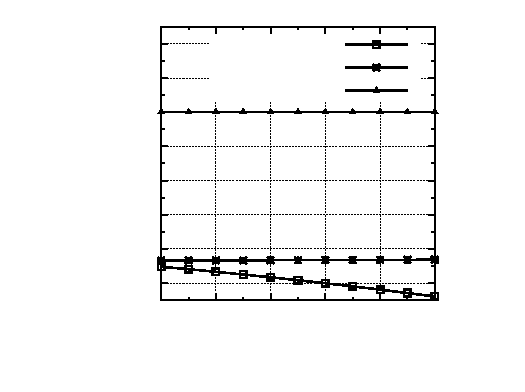
\includegraphics{figures/prmom-pol/prmom-pol}}%
    \gplfronttext
  \end{picture}%
\endgroup

\caption{The Born energy and components thereof for the perturbation of propylbenzene to benzyl methyl ether. Top left: energy trajectory; top right: charge trajectories; bottom left: volume trajectories; bottom right: electrostatic trajectories.}
\label{prmom}
\end{figure}


PhPr $\longrightarrow$ BzOCH$_3$ Results for the perturbation of propylbenzene to benzyl methyl ether are given in \cref{prmom}. Key atoms were determined for this test case to be the carbon perturbed to oxygen, the methyl carbon, and the hydrogens perturbed to dummy atoms. This test case was notable in that it involved oxygen and simultaneous perturbation to two vicinal dummy atoms. Nevertheless, trajectories were smooth and consistent throughout the course of the perturbation for the total Born energy of the system, atomic charges, volumes, and electrostatic contributions, and trends therein were unremarkable. Volumes (\cref{prmom}, bottom left) were stable despite vicinal hydrogen to dummy perturbations, with dummy atoms reaching the minimum volume of 1.0 \AA$^3$ near $\lambda = 0.7$ and electrostatic contribution for the methylene hydrogens to dummy remaining constant at zero. The perturbation yielded an overall Born energy change $\Delta G_{ \textrm{Born}}$ of $-2.1$ kcal/mol.

PhCH$_3$ $\longrightarrow$ PhCF$_3$. Results for the perturbation of toluene to (trifluoromethyl)benzene are given in \cref{ch3cf3}. Key atoms were determined to be the methyl hydrogens perturbed to fluorines and the carbon to which they were attached, as well as the substituted aromatic carbon. Once more, this example was particularly interesting as a test case because of the large differences in charge and volume between the initial and final state. Illustrating this is the volume trajectories graph (\cref{ch3cf3}, bottom left), which shows how the volume of the methyl carbon quickly vanished by $\lambda = 0.7$ as it became eclipsed by the three growing fluorines. Volume of the substituted aromatic carbon, the atom of the interest farthest from the fluorines, remained unchanged. Charge perturbations (\cref{ch3cf3}, top right) were large, most dramatically for the methyl carbon, which developed significant positive charge throughout the course of the simulation, owing to the large change in electronegativity between methyl and trifluoromethyl groups. Electrostatic contribution for methyl hydrogens was scaled linearly from zero, yielding a smooth overall Born energy trajectory and $\Delta G_{ \textrm{Born}}$ of $+0.75$ kcal/mol for the perturbation.


\begin{figure}[t!]
\centering
PhCH$_3$ $\longrightarrow$ PhCF$_3$\\
% GNUPLOT: LaTeX picture with Postscript
\begingroup
  \makeatletter
  \providecommand\color[2][]{%
    \GenericError{(gnuplot) \space\space\space\@spaces}{%
      Package color not loaded in conjunction with
      terminal option `colourtext'%
    }{See the gnuplot documentation for explanation.%
    }{Either use 'blacktext' in gnuplot or load the package
      color.sty in LaTeX.}%
    \renewcommand\color[2][]{}%
  }%
  \providecommand\includegraphics[2][]{%
    \GenericError{(gnuplot) \space\space\space\@spaces}{%
      Package graphicx or graphics not loaded%
    }{See the gnuplot documentation for explanation.%
    }{The gnuplot epslatex terminal needs graphicx.sty or graphics.sty.}%
    \renewcommand\includegraphics[2][]{}%
  }%
  \providecommand\rotatebox[2]{#2}%
  \@ifundefined{ifGPcolor}{%
    \newif\ifGPcolor
    \GPcolortrue
  }{}%
  \@ifundefined{ifGPblacktext}{%
    \newif\ifGPblacktext
    \GPblacktextfalse
  }{}%
  % define a \g@addto@macro without @ in the name:
  \let\gplgaddtomacro\g@addto@macro
  % define empty templates for all commands taking text:
  \gdef\gplbacktext{}%
  \gdef\gplfronttext{}%
  \makeatother
  \ifGPblacktext
    % no textcolor at all
    \def\colorrgb#1{}%
    \def\colorgray#1{}%
  \else
    % gray or color?
    \ifGPcolor
      \def\colorrgb#1{\color[rgb]{#1}}%
      \def\colorgray#1{\color[gray]{#1}}%
      \expandafter\def\csname LTw\endcsname{\color{white}}%
      \expandafter\def\csname LTb\endcsname{\color{black}}%
      \expandafter\def\csname LTa\endcsname{\color{black}}%
      \expandafter\def\csname LT0\endcsname{\color[rgb]{1,0,0}}%
      \expandafter\def\csname LT1\endcsname{\color[rgb]{0,1,0}}%
      \expandafter\def\csname LT2\endcsname{\color[rgb]{0,0,1}}%
      \expandafter\def\csname LT3\endcsname{\color[rgb]{1,0,1}}%
      \expandafter\def\csname LT4\endcsname{\color[rgb]{0,1,1}}%
      \expandafter\def\csname LT5\endcsname{\color[rgb]{1,1,0}}%
      \expandafter\def\csname LT6\endcsname{\color[rgb]{0,0,0}}%
      \expandafter\def\csname LT7\endcsname{\color[rgb]{1,0.3,0}}%
      \expandafter\def\csname LT8\endcsname{\color[rgb]{0.5,0.5,0.5}}%
    \else
      % gray
      \def\colorrgb#1{\color{black}}%
      \def\colorgray#1{\color[gray]{#1}}%
      \expandafter\def\csname LTw\endcsname{\color{white}}%
      \expandafter\def\csname LTb\endcsname{\color{black}}%
      \expandafter\def\csname LTa\endcsname{\color{black}}%
      \expandafter\def\csname LT0\endcsname{\color{black}}%
      \expandafter\def\csname LT1\endcsname{\color{black}}%
      \expandafter\def\csname LT2\endcsname{\color{black}}%
      \expandafter\def\csname LT3\endcsname{\color{black}}%
      \expandafter\def\csname LT4\endcsname{\color{black}}%
      \expandafter\def\csname LT5\endcsname{\color{black}}%
      \expandafter\def\csname LT6\endcsname{\color{black}}%
      \expandafter\def\csname LT7\endcsname{\color{black}}%
      \expandafter\def\csname LT8\endcsname{\color{black}}%
    \fi
  \fi
  \setlength{\unitlength}{0.0500bp}%
  \begin{picture}(5040.00,3772.00)%
    \gplgaddtomacro\gplbacktext{%
      \csname LTb\endcsname%
      \put(1415,880){\makebox(0,0)[r]{\strut{}-2.6}}%
      \csname LTb\endcsname%
      \put(1415,1405){\makebox(0,0)[r]{\strut{}-2.4}}%
      \csname LTb\endcsname%
      \put(1415,1931){\makebox(0,0)[r]{\strut{}-2.2}}%
      \csname LTb\endcsname%
      \put(1415,2456){\makebox(0,0)[r]{\strut{}-2}}%
      \csname LTb\endcsname%
      \put(1415,2982){\makebox(0,0)[r]{\strut{}-1.8}}%
      \csname LTb\endcsname%
      \put(1415,3507){\makebox(0,0)[r]{\strut{}-1.6}}%
      \csname LTb\endcsname%
      \put(1547,660){\makebox(0,0){\strut{} 0}}%
      \csname LTb\endcsname%
      \put(2072,660){\makebox(0,0){\strut{} 0.2}}%
      \csname LTb\endcsname%
      \put(2598,660){\makebox(0,0){\strut{} 0.4}}%
      \csname LTb\endcsname%
      \put(3123,660){\makebox(0,0){\strut{} 0.6}}%
      \csname LTb\endcsname%
      \put(3649,660){\makebox(0,0){\strut{} 0.8}}%
      \csname LTb\endcsname%
      \put(4174,660){\makebox(0,0){\strut{} 1}}%
      \csname LTb\endcsname%
      \put(645,2193){\rotatebox{-270}{\makebox(0,0){\strut{}Born energy (kcal/mol)}}}%
      \put(2860,330){\makebox(0,0){\strut{}$\lambda$}}%
    }%
    \gplgaddtomacro\gplfronttext{%
    }%
    \gplbacktext
    \put(0,0){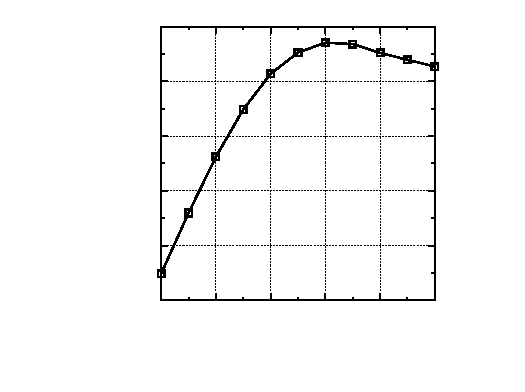
\includegraphics{figures/chf3-en/chf3-en}}%
    \gplfronttext
  \end{picture}%
\endgroup
\hspace*{-1.3cm}% GNUPLOT: LaTeX picture with Postscript
\begingroup
  \makeatletter
  \providecommand\color[2][]{%
    \GenericError{(gnuplot) \space\space\space\@spaces}{%
      Package color not loaded in conjunction with
      terminal option `colourtext'%
    }{See the gnuplot documentation for explanation.%
    }{Either use 'blacktext' in gnuplot or load the package
      color.sty in LaTeX.}%
    \renewcommand\color[2][]{}%
  }%
  \providecommand\includegraphics[2][]{%
    \GenericError{(gnuplot) \space\space\space\@spaces}{%
      Package graphicx or graphics not loaded%
    }{See the gnuplot documentation for explanation.%
    }{The gnuplot epslatex terminal needs graphicx.sty or graphics.sty.}%
    \renewcommand\includegraphics[2][]{}%
  }%
  \providecommand\rotatebox[2]{#2}%
  \@ifundefined{ifGPcolor}{%
    \newif\ifGPcolor
    \GPcolortrue
  }{}%
  \@ifundefined{ifGPblacktext}{%
    \newif\ifGPblacktext
    \GPblacktextfalse
  }{}%
  % define a \g@addto@macro without @ in the name:
  \let\gplgaddtomacro\g@addto@macro
  % define empty templates for all commands taking text:
  \gdef\gplbacktext{}%
  \gdef\gplfronttext{}%
  \makeatother
  \ifGPblacktext
    % no textcolor at all
    \def\colorrgb#1{}%
    \def\colorgray#1{}%
  \else
    % gray or color?
    \ifGPcolor
      \def\colorrgb#1{\color[rgb]{#1}}%
      \def\colorgray#1{\color[gray]{#1}}%
      \expandafter\def\csname LTw\endcsname{\color{white}}%
      \expandafter\def\csname LTb\endcsname{\color{black}}%
      \expandafter\def\csname LTa\endcsname{\color{black}}%
      \expandafter\def\csname LT0\endcsname{\color[rgb]{1,0,0}}%
      \expandafter\def\csname LT1\endcsname{\color[rgb]{0,1,0}}%
      \expandafter\def\csname LT2\endcsname{\color[rgb]{0,0,1}}%
      \expandafter\def\csname LT3\endcsname{\color[rgb]{1,0,1}}%
      \expandafter\def\csname LT4\endcsname{\color[rgb]{0,1,1}}%
      \expandafter\def\csname LT5\endcsname{\color[rgb]{1,1,0}}%
      \expandafter\def\csname LT6\endcsname{\color[rgb]{0,0,0}}%
      \expandafter\def\csname LT7\endcsname{\color[rgb]{1,0.3,0}}%
      \expandafter\def\csname LT8\endcsname{\color[rgb]{0.5,0.5,0.5}}%
    \else
      % gray
      \def\colorrgb#1{\color{black}}%
      \def\colorgray#1{\color[gray]{#1}}%
      \expandafter\def\csname LTw\endcsname{\color{white}}%
      \expandafter\def\csname LTb\endcsname{\color{black}}%
      \expandafter\def\csname LTa\endcsname{\color{black}}%
      \expandafter\def\csname LT0\endcsname{\color{black}}%
      \expandafter\def\csname LT1\endcsname{\color{black}}%
      \expandafter\def\csname LT2\endcsname{\color{black}}%
      \expandafter\def\csname LT3\endcsname{\color{black}}%
      \expandafter\def\csname LT4\endcsname{\color{black}}%
      \expandafter\def\csname LT5\endcsname{\color{black}}%
      \expandafter\def\csname LT6\endcsname{\color{black}}%
      \expandafter\def\csname LT7\endcsname{\color{black}}%
      \expandafter\def\csname LT8\endcsname{\color{black}}%
    \fi
  \fi
  \setlength{\unitlength}{0.0500bp}%
  \begin{picture}(5040.00,3772.00)%
    \gplgaddtomacro\gplbacktext{%
      \csname LTb\endcsname%
      \put(1415,1143){\makebox(0,0)[r]{\strut{}-0.2}}%
      \csname LTb\endcsname%
      \put(1415,1668){\makebox(0,0)[r]{\strut{} 0}}%
      \csname LTb\endcsname%
      \put(1415,2194){\makebox(0,0)[r]{\strut{} 0.2}}%
      \csname LTb\endcsname%
      \put(1415,2719){\makebox(0,0)[r]{\strut{} 0.4}}%
      \csname LTb\endcsname%
      \put(1415,3244){\makebox(0,0)[r]{\strut{} 0.6}}%
      \csname LTb\endcsname%
      \put(1547,660){\makebox(0,0){\strut{} 0}}%
      \csname LTb\endcsname%
      \put(2072,660){\makebox(0,0){\strut{} 0.2}}%
      \csname LTb\endcsname%
      \put(2598,660){\makebox(0,0){\strut{} 0.4}}%
      \csname LTb\endcsname%
      \put(3123,660){\makebox(0,0){\strut{} 0.6}}%
      \csname LTb\endcsname%
      \put(3649,660){\makebox(0,0){\strut{} 0.8}}%
      \csname LTb\endcsname%
      \put(4174,660){\makebox(0,0){\strut{} 1}}%
      \put(645,2193){\rotatebox{-270}{\makebox(0,0){\strut{}charge}}}%
      \put(2860,330){\makebox(0,0){\strut{}$\lambda$}}%
    }%
    \gplgaddtomacro\gplfronttext{%
      \csname LTb\endcsname%
      \put(3187,3334){\makebox(0,0)[r]{\strut{}C}}%
      \csname LTb\endcsname%
      \put(3187,3114){\makebox(0,0)[r]{\strut{}CA}}%
      \csname LTb\endcsname%
      \put(3187,2894){\makebox(0,0)[r]{\strut{}H $\rightarrow$ F}}%
    }%
    \gplbacktext
    \put(0,0){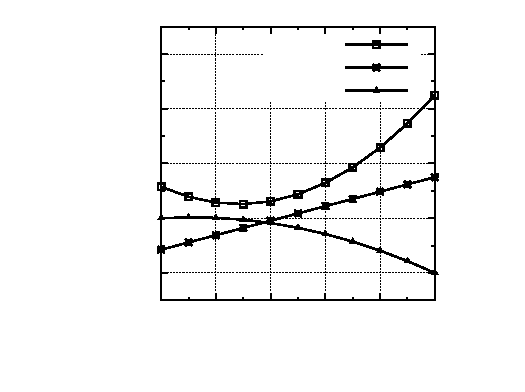
\includegraphics{figures/chf3-charge/chf3-charge}}%
    \gplfronttext
  \end{picture}%
\endgroup
\\
% GNUPLOT: LaTeX picture with Postscript
\begingroup
  \makeatletter
  \providecommand\color[2][]{%
    \GenericError{(gnuplot) \space\space\space\@spaces}{%
      Package color not loaded in conjunction with
      terminal option `colourtext'%
    }{See the gnuplot documentation for explanation.%
    }{Either use 'blacktext' in gnuplot or load the package
      color.sty in LaTeX.}%
    \renewcommand\color[2][]{}%
  }%
  \providecommand\includegraphics[2][]{%
    \GenericError{(gnuplot) \space\space\space\@spaces}{%
      Package graphicx or graphics not loaded%
    }{See the gnuplot documentation for explanation.%
    }{The gnuplot epslatex terminal needs graphicx.sty or graphics.sty.}%
    \renewcommand\includegraphics[2][]{}%
  }%
  \providecommand\rotatebox[2]{#2}%
  \@ifundefined{ifGPcolor}{%
    \newif\ifGPcolor
    \GPcolortrue
  }{}%
  \@ifundefined{ifGPblacktext}{%
    \newif\ifGPblacktext
    \GPblacktextfalse
  }{}%
  % define a \g@addto@macro without @ in the name:
  \let\gplgaddtomacro\g@addto@macro
  % define empty templates for all commands taking text:
  \gdef\gplbacktext{}%
  \gdef\gplfronttext{}%
  \makeatother
  \ifGPblacktext
    % no textcolor at all
    \def\colorrgb#1{}%
    \def\colorgray#1{}%
  \else
    % gray or color?
    \ifGPcolor
      \def\colorrgb#1{\color[rgb]{#1}}%
      \def\colorgray#1{\color[gray]{#1}}%
      \expandafter\def\csname LTw\endcsname{\color{white}}%
      \expandafter\def\csname LTb\endcsname{\color{black}}%
      \expandafter\def\csname LTa\endcsname{\color{black}}%
      \expandafter\def\csname LT0\endcsname{\color[rgb]{1,0,0}}%
      \expandafter\def\csname LT1\endcsname{\color[rgb]{0,1,0}}%
      \expandafter\def\csname LT2\endcsname{\color[rgb]{0,0,1}}%
      \expandafter\def\csname LT3\endcsname{\color[rgb]{1,0,1}}%
      \expandafter\def\csname LT4\endcsname{\color[rgb]{0,1,1}}%
      \expandafter\def\csname LT5\endcsname{\color[rgb]{1,1,0}}%
      \expandafter\def\csname LT6\endcsname{\color[rgb]{0,0,0}}%
      \expandafter\def\csname LT7\endcsname{\color[rgb]{1,0.3,0}}%
      \expandafter\def\csname LT8\endcsname{\color[rgb]{0.5,0.5,0.5}}%
    \else
      % gray
      \def\colorrgb#1{\color{black}}%
      \def\colorgray#1{\color[gray]{#1}}%
      \expandafter\def\csname LTw\endcsname{\color{white}}%
      \expandafter\def\csname LTb\endcsname{\color{black}}%
      \expandafter\def\csname LTa\endcsname{\color{black}}%
      \expandafter\def\csname LT0\endcsname{\color{black}}%
      \expandafter\def\csname LT1\endcsname{\color{black}}%
      \expandafter\def\csname LT2\endcsname{\color{black}}%
      \expandafter\def\csname LT3\endcsname{\color{black}}%
      \expandafter\def\csname LT4\endcsname{\color{black}}%
      \expandafter\def\csname LT5\endcsname{\color{black}}%
      \expandafter\def\csname LT6\endcsname{\color{black}}%
      \expandafter\def\csname LT7\endcsname{\color{black}}%
      \expandafter\def\csname LT8\endcsname{\color{black}}%
    \fi
  \fi
  \setlength{\unitlength}{0.0500bp}%
  \begin{picture}(5040.00,3772.00)%
    \gplgaddtomacro\gplbacktext{%
      \csname LTb\endcsname%
      \put(1349,880){\makebox(0,0)[r]{\strut{} 0}}%
      \csname LTb\endcsname%
      \put(1349,1208){\makebox(0,0)[r]{\strut{} 5}}%
      \csname LTb\endcsname%
      \put(1349,1537){\makebox(0,0)[r]{\strut{} 10}}%
      \csname LTb\endcsname%
      \put(1349,1865){\makebox(0,0)[r]{\strut{} 15}}%
      \csname LTb\endcsname%
      \put(1349,2194){\makebox(0,0)[r]{\strut{} 20}}%
      \csname LTb\endcsname%
      \put(1349,2522){\makebox(0,0)[r]{\strut{} 25}}%
      \csname LTb\endcsname%
      \put(1349,2850){\makebox(0,0)[r]{\strut{} 30}}%
      \csname LTb\endcsname%
      \put(1349,3179){\makebox(0,0)[r]{\strut{} 35}}%
      \csname LTb\endcsname%
      \put(1349,3507){\makebox(0,0)[r]{\strut{} 40}}%
      \csname LTb\endcsname%
      \put(1481,660){\makebox(0,0){\strut{} 0}}%
      \csname LTb\endcsname%
      \put(2006,660){\makebox(0,0){\strut{} 0.2}}%
      \csname LTb\endcsname%
      \put(2532,660){\makebox(0,0){\strut{} 0.4}}%
      \csname LTb\endcsname%
      \put(3057,660){\makebox(0,0){\strut{} 0.6}}%
      \csname LTb\endcsname%
      \put(3583,660){\makebox(0,0){\strut{} 0.8}}%
      \csname LTb\endcsname%
      \put(4108,660){\makebox(0,0){\strut{} 1}}%
      \put(711,2193){\rotatebox{-270}{\makebox(0,0){\strut{}volume (\AA$^{3}$)}}}%
      \put(2794,330){\makebox(0,0){\strut{}$\lambda$}}%
    }%
    \gplgaddtomacro\gplfronttext{%
      \csname LTb\endcsname%
      \put(3121,3334){\makebox(0,0)[r]{\strut{}C}}%
      \csname LTb\endcsname%
      \put(3121,3114){\makebox(0,0)[r]{\strut{}CA}}%
      \csname LTb\endcsname%
      \put(3121,2894){\makebox(0,0)[r]{\strut{}H $\rightarrow$ F}}%
    }%
    \gplbacktext
    \put(0,0){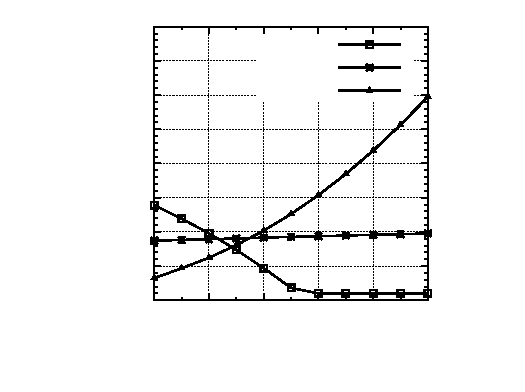
\includegraphics{figures/chf3-vol/chf3-vol}}%
    \gplfronttext
  \end{picture}%
\endgroup
\hspace*{-1.3cm}% GNUPLOT: LaTeX picture with Postscript
\begingroup
  \makeatletter
  \providecommand\color[2][]{%
    \GenericError{(gnuplot) \space\space\space\@spaces}{%
      Package color not loaded in conjunction with
      terminal option `colourtext'%
    }{See the gnuplot documentation for explanation.%
    }{Either use 'blacktext' in gnuplot or load the package
      color.sty in LaTeX.}%
    \renewcommand\color[2][]{}%
  }%
  \providecommand\includegraphics[2][]{%
    \GenericError{(gnuplot) \space\space\space\@spaces}{%
      Package graphicx or graphics not loaded%
    }{See the gnuplot documentation for explanation.%
    }{The gnuplot epslatex terminal needs graphicx.sty or graphics.sty.}%
    \renewcommand\includegraphics[2][]{}%
  }%
  \providecommand\rotatebox[2]{#2}%
  \@ifundefined{ifGPcolor}{%
    \newif\ifGPcolor
    \GPcolortrue
  }{}%
  \@ifundefined{ifGPblacktext}{%
    \newif\ifGPblacktext
    \GPblacktextfalse
  }{}%
  % define a \g@addto@macro without @ in the name:
  \let\gplgaddtomacro\g@addto@macro
  % define empty templates for all commands taking text:
  \gdef\gplbacktext{}%
  \gdef\gplfronttext{}%
  \makeatother
  \ifGPblacktext
    % no textcolor at all
    \def\colorrgb#1{}%
    \def\colorgray#1{}%
  \else
    % gray or color?
    \ifGPcolor
      \def\colorrgb#1{\color[rgb]{#1}}%
      \def\colorgray#1{\color[gray]{#1}}%
      \expandafter\def\csname LTw\endcsname{\color{white}}%
      \expandafter\def\csname LTb\endcsname{\color{black}}%
      \expandafter\def\csname LTa\endcsname{\color{black}}%
      \expandafter\def\csname LT0\endcsname{\color[rgb]{1,0,0}}%
      \expandafter\def\csname LT1\endcsname{\color[rgb]{0,1,0}}%
      \expandafter\def\csname LT2\endcsname{\color[rgb]{0,0,1}}%
      \expandafter\def\csname LT3\endcsname{\color[rgb]{1,0,1}}%
      \expandafter\def\csname LT4\endcsname{\color[rgb]{0,1,1}}%
      \expandafter\def\csname LT5\endcsname{\color[rgb]{1,1,0}}%
      \expandafter\def\csname LT6\endcsname{\color[rgb]{0,0,0}}%
      \expandafter\def\csname LT7\endcsname{\color[rgb]{1,0.3,0}}%
      \expandafter\def\csname LT8\endcsname{\color[rgb]{0.5,0.5,0.5}}%
    \else
      % gray
      \def\colorrgb#1{\color{black}}%
      \def\colorgray#1{\color[gray]{#1}}%
      \expandafter\def\csname LTw\endcsname{\color{white}}%
      \expandafter\def\csname LTb\endcsname{\color{black}}%
      \expandafter\def\csname LTa\endcsname{\color{black}}%
      \expandafter\def\csname LT0\endcsname{\color{black}}%
      \expandafter\def\csname LT1\endcsname{\color{black}}%
      \expandafter\def\csname LT2\endcsname{\color{black}}%
      \expandafter\def\csname LT3\endcsname{\color{black}}%
      \expandafter\def\csname LT4\endcsname{\color{black}}%
      \expandafter\def\csname LT5\endcsname{\color{black}}%
      \expandafter\def\csname LT6\endcsname{\color{black}}%
      \expandafter\def\csname LT7\endcsname{\color{black}}%
      \expandafter\def\csname LT8\endcsname{\color{black}}%
    \fi
  \fi
  \setlength{\unitlength}{0.0500bp}%
  \begin{picture}(5040.00,3772.00)%
    \gplgaddtomacro\gplbacktext{%
      \csname LTb\endcsname%
      \put(1415,880){\makebox(0,0)[r]{\strut{}-140}}%
      \csname LTb\endcsname%
      \put(1415,1255){\makebox(0,0)[r]{\strut{}-120}}%
      \csname LTb\endcsname%
      \put(1415,1631){\makebox(0,0)[r]{\strut{}-100}}%
      \csname LTb\endcsname%
      \put(1415,2006){\makebox(0,0)[r]{\strut{}-80}}%
      \csname LTb\endcsname%
      \put(1415,2381){\makebox(0,0)[r]{\strut{}-60}}%
      \csname LTb\endcsname%
      \put(1415,2756){\makebox(0,0)[r]{\strut{}-40}}%
      \csname LTb\endcsname%
      \put(1415,3132){\makebox(0,0)[r]{\strut{}-20}}%
      \csname LTb\endcsname%
      \put(1415,3507){\makebox(0,0)[r]{\strut{} 0}}%
      \csname LTb\endcsname%
      \put(1547,660){\makebox(0,0){\strut{} 0}}%
      \csname LTb\endcsname%
      \put(2072,660){\makebox(0,0){\strut{} 0.2}}%
      \csname LTb\endcsname%
      \put(2598,660){\makebox(0,0){\strut{} 0.4}}%
      \csname LTb\endcsname%
      \put(3123,660){\makebox(0,0){\strut{} 0.6}}%
      \csname LTb\endcsname%
      \put(3649,660){\makebox(0,0){\strut{} 0.8}}%
      \csname LTb\endcsname%
      \put(4174,660){\makebox(0,0){\strut{} 1}}%
      \put(645,2193){\rotatebox{-270}{\makebox(0,0){\strut{}$G^\prime_{\textrm{pol},i}$}}}%
      \put(2860,330){\makebox(0,0){\strut{}$\lambda$}}%
    }%
    \gplgaddtomacro\gplfronttext{%
      \csname LTb\endcsname%
      \put(3187,3334){\makebox(0,0)[r]{\strut{}C}}%
      \csname LTb\endcsname%
      \put(3187,3114){\makebox(0,0)[r]{\strut{}CA}}%
      \csname LTb\endcsname%
      \put(3187,2894){\makebox(0,0)[r]{\strut{}H $\rightarrow$ F}}%
    }%
    \gplbacktext
    \put(0,0){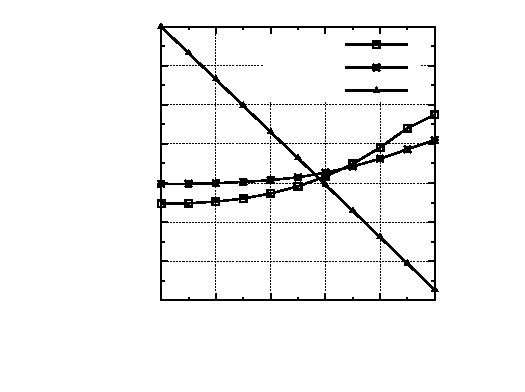
\includegraphics{figures/chf3-pol/chf3-pol}}%
    \gplfronttext
  \end{picture}%
\endgroup

\caption{The Born energy and components thereof for the perturbation of toluene to (trifluoromethyl)benzene. Top left: energy trajectory; top right: charge trajectories; bottom left: volume trajectories; bottom right: electrostatic trajectories.}
\label{ch3cf3}
\end{figure}

\begin{figure}[t!]
\centering
PhC(O)CH$_3$  $\longrightarrow$ PhNO$_2$\\
% GNUPLOT: LaTeX picture with Postscript
\begingroup
  \makeatletter
  \providecommand\color[2][]{%
    \GenericError{(gnuplot) \space\space\space\@spaces}{%
      Package color not loaded in conjunction with
      terminal option `colourtext'%
    }{See the gnuplot documentation for explanation.%
    }{Either use 'blacktext' in gnuplot or load the package
      color.sty in LaTeX.}%
    \renewcommand\color[2][]{}%
  }%
  \providecommand\includegraphics[2][]{%
    \GenericError{(gnuplot) \space\space\space\@spaces}{%
      Package graphicx or graphics not loaded%
    }{See the gnuplot documentation for explanation.%
    }{The gnuplot epslatex terminal needs graphicx.sty or graphics.sty.}%
    \renewcommand\includegraphics[2][]{}%
  }%
  \providecommand\rotatebox[2]{#2}%
  \@ifundefined{ifGPcolor}{%
    \newif\ifGPcolor
    \GPcolortrue
  }{}%
  \@ifundefined{ifGPblacktext}{%
    \newif\ifGPblacktext
    \GPblacktextfalse
  }{}%
  % define a \g@addto@macro without @ in the name:
  \let\gplgaddtomacro\g@addto@macro
  % define empty templates for all commands taking text:
  \gdef\gplbacktext{}%
  \gdef\gplfronttext{}%
  \makeatother
  \ifGPblacktext
    % no textcolor at all
    \def\colorrgb#1{}%
    \def\colorgray#1{}%
  \else
    % gray or color?
    \ifGPcolor
      \def\colorrgb#1{\color[rgb]{#1}}%
      \def\colorgray#1{\color[gray]{#1}}%
      \expandafter\def\csname LTw\endcsname{\color{white}}%
      \expandafter\def\csname LTb\endcsname{\color{black}}%
      \expandafter\def\csname LTa\endcsname{\color{black}}%
      \expandafter\def\csname LT0\endcsname{\color[rgb]{1,0,0}}%
      \expandafter\def\csname LT1\endcsname{\color[rgb]{0,1,0}}%
      \expandafter\def\csname LT2\endcsname{\color[rgb]{0,0,1}}%
      \expandafter\def\csname LT3\endcsname{\color[rgb]{1,0,1}}%
      \expandafter\def\csname LT4\endcsname{\color[rgb]{0,1,1}}%
      \expandafter\def\csname LT5\endcsname{\color[rgb]{1,1,0}}%
      \expandafter\def\csname LT6\endcsname{\color[rgb]{0,0,0}}%
      \expandafter\def\csname LT7\endcsname{\color[rgb]{1,0.3,0}}%
      \expandafter\def\csname LT8\endcsname{\color[rgb]{0.5,0.5,0.5}}%
    \else
      % gray
      \def\colorrgb#1{\color{black}}%
      \def\colorgray#1{\color[gray]{#1}}%
      \expandafter\def\csname LTw\endcsname{\color{white}}%
      \expandafter\def\csname LTb\endcsname{\color{black}}%
      \expandafter\def\csname LTa\endcsname{\color{black}}%
      \expandafter\def\csname LT0\endcsname{\color{black}}%
      \expandafter\def\csname LT1\endcsname{\color{black}}%
      \expandafter\def\csname LT2\endcsname{\color{black}}%
      \expandafter\def\csname LT3\endcsname{\color{black}}%
      \expandafter\def\csname LT4\endcsname{\color{black}}%
      \expandafter\def\csname LT5\endcsname{\color{black}}%
      \expandafter\def\csname LT6\endcsname{\color{black}}%
      \expandafter\def\csname LT7\endcsname{\color{black}}%
      \expandafter\def\csname LT8\endcsname{\color{black}}%
    \fi
  \fi
  \setlength{\unitlength}{0.0500bp}%
  \begin{picture}(5040.00,3772.00)%
    \gplgaddtomacro\gplbacktext{%
      \csname LTb\endcsname%
      \put(1415,880){\makebox(0,0)[r]{\strut{}-7.4}}%
      \csname LTb\endcsname%
      \put(1415,1255){\makebox(0,0)[r]{\strut{}-7.2}}%
      \csname LTb\endcsname%
      \put(1415,1631){\makebox(0,0)[r]{\strut{}-7}}%
      \csname LTb\endcsname%
      \put(1415,2006){\makebox(0,0)[r]{\strut{}-6.8}}%
      \csname LTb\endcsname%
      \put(1415,2381){\makebox(0,0)[r]{\strut{}-6.6}}%
      \csname LTb\endcsname%
      \put(1415,2756){\makebox(0,0)[r]{\strut{}-6.4}}%
      \csname LTb\endcsname%
      \put(1415,3132){\makebox(0,0)[r]{\strut{}-6.2}}%
      \csname LTb\endcsname%
      \put(1415,3507){\makebox(0,0)[r]{\strut{}-6}}%
      \csname LTb\endcsname%
      \put(1547,660){\makebox(0,0){\strut{} 0}}%
      \csname LTb\endcsname%
      \put(2072,660){\makebox(0,0){\strut{} 0.2}}%
      \csname LTb\endcsname%
      \put(2598,660){\makebox(0,0){\strut{} 0.4}}%
      \csname LTb\endcsname%
      \put(3123,660){\makebox(0,0){\strut{} 0.6}}%
      \csname LTb\endcsname%
      \put(3649,660){\makebox(0,0){\strut{} 0.8}}%
      \csname LTb\endcsname%
      \put(4174,660){\makebox(0,0){\strut{} 1}}%
      \csname LTb\endcsname%
      \put(645,2193){\rotatebox{-270}{\makebox(0,0){\strut{}Born energy (kcal/mol)}}}%
      \put(2860,330){\makebox(0,0){\strut{}$\lambda$}}%
    }%
    \gplgaddtomacro\gplfronttext{%
    }%
    \gplbacktext
    \put(0,0){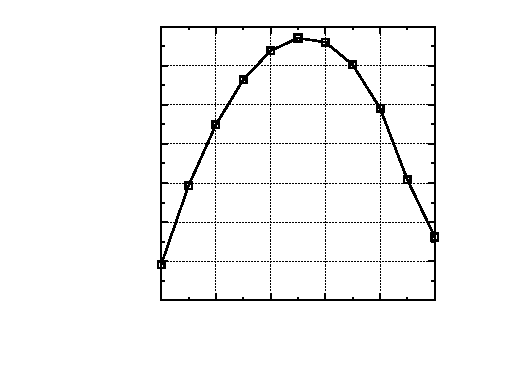
\includegraphics{figures/no2-en/no2-en}}%
    \gplfronttext
  \end{picture}%
\endgroup
\hspace*{-1.3cm}% GNUPLOT: LaTeX picture with Postscript
\begingroup
  \makeatletter
  \providecommand\color[2][]{%
    \GenericError{(gnuplot) \space\space\space\@spaces}{%
      Package color not loaded in conjunction with
      terminal option `colourtext'%
    }{See the gnuplot documentation for explanation.%
    }{Either use 'blacktext' in gnuplot or load the package
      color.sty in LaTeX.}%
    \renewcommand\color[2][]{}%
  }%
  \providecommand\includegraphics[2][]{%
    \GenericError{(gnuplot) \space\space\space\@spaces}{%
      Package graphicx or graphics not loaded%
    }{See the gnuplot documentation for explanation.%
    }{The gnuplot epslatex terminal needs graphicx.sty or graphics.sty.}%
    \renewcommand\includegraphics[2][]{}%
  }%
  \providecommand\rotatebox[2]{#2}%
  \@ifundefined{ifGPcolor}{%
    \newif\ifGPcolor
    \GPcolortrue
  }{}%
  \@ifundefined{ifGPblacktext}{%
    \newif\ifGPblacktext
    \GPblacktextfalse
  }{}%
  % define a \g@addto@macro without @ in the name:
  \let\gplgaddtomacro\g@addto@macro
  % define empty templates for all commands taking text:
  \gdef\gplbacktext{}%
  \gdef\gplfronttext{}%
  \makeatother
  \ifGPblacktext
    % no textcolor at all
    \def\colorrgb#1{}%
    \def\colorgray#1{}%
  \else
    % gray or color?
    \ifGPcolor
      \def\colorrgb#1{\color[rgb]{#1}}%
      \def\colorgray#1{\color[gray]{#1}}%
      \expandafter\def\csname LTw\endcsname{\color{white}}%
      \expandafter\def\csname LTb\endcsname{\color{black}}%
      \expandafter\def\csname LTa\endcsname{\color{black}}%
      \expandafter\def\csname LT0\endcsname{\color[rgb]{1,0,0}}%
      \expandafter\def\csname LT1\endcsname{\color[rgb]{0,1,0}}%
      \expandafter\def\csname LT2\endcsname{\color[rgb]{0,0,1}}%
      \expandafter\def\csname LT3\endcsname{\color[rgb]{1,0,1}}%
      \expandafter\def\csname LT4\endcsname{\color[rgb]{0,1,1}}%
      \expandafter\def\csname LT5\endcsname{\color[rgb]{1,1,0}}%
      \expandafter\def\csname LT6\endcsname{\color[rgb]{0,0,0}}%
      \expandafter\def\csname LT7\endcsname{\color[rgb]{1,0.3,0}}%
      \expandafter\def\csname LT8\endcsname{\color[rgb]{0.5,0.5,0.5}}%
    \else
      % gray
      \def\colorrgb#1{\color{black}}%
      \def\colorgray#1{\color[gray]{#1}}%
      \expandafter\def\csname LTw\endcsname{\color{white}}%
      \expandafter\def\csname LTb\endcsname{\color{black}}%
      \expandafter\def\csname LTa\endcsname{\color{black}}%
      \expandafter\def\csname LT0\endcsname{\color{black}}%
      \expandafter\def\csname LT1\endcsname{\color{black}}%
      \expandafter\def\csname LT2\endcsname{\color{black}}%
      \expandafter\def\csname LT3\endcsname{\color{black}}%
      \expandafter\def\csname LT4\endcsname{\color{black}}%
      \expandafter\def\csname LT5\endcsname{\color{black}}%
      \expandafter\def\csname LT6\endcsname{\color{black}}%
      \expandafter\def\csname LT7\endcsname{\color{black}}%
      \expandafter\def\csname LT8\endcsname{\color{black}}%
    \fi
  \fi
  \setlength{\unitlength}{0.0500bp}%
  \begin{picture}(5040.00,3772.00)%
    \gplgaddtomacro\gplbacktext{%
      \csname LTb\endcsname%
      \put(1415,880){\makebox(0,0)[r]{\strut{}-0.5}}%
      \csname LTb\endcsname%
      \put(1415,1537){\makebox(0,0)[r]{\strut{} 0}}%
      \csname LTb\endcsname%
      \put(1415,2194){\makebox(0,0)[r]{\strut{} 0.5}}%
      \csname LTb\endcsname%
      \put(1415,2850){\makebox(0,0)[r]{\strut{} 1}}%
      \csname LTb\endcsname%
      \put(1415,3507){\makebox(0,0)[r]{\strut{} 1.5}}%
      \csname LTb\endcsname%
      \put(1547,660){\makebox(0,0){\strut{} 0}}%
      \csname LTb\endcsname%
      \put(2072,660){\makebox(0,0){\strut{} 0.2}}%
      \csname LTb\endcsname%
      \put(2598,660){\makebox(0,0){\strut{} 0.4}}%
      \csname LTb\endcsname%
      \put(3123,660){\makebox(0,0){\strut{} 0.6}}%
      \csname LTb\endcsname%
      \put(3649,660){\makebox(0,0){\strut{} 0.8}}%
      \csname LTb\endcsname%
      \put(4174,660){\makebox(0,0){\strut{} 1}}%
      \put(645,2193){\rotatebox{-270}{\makebox(0,0){\strut{}charge}}}%
      \put(2860,330){\makebox(0,0){\strut{}$\lambda$}}%
    }%
    \gplgaddtomacro\gplfronttext{%
      \csname LTb\endcsname%
      \put(3187,3334){\makebox(0,0)[r]{\strut{}C $\rightarrow$ O}}%
      \csname LTb\endcsname%
      \put(3187,3114){\makebox(0,0)[r]{\strut{}C $\rightarrow$ N}}%
      \csname LTb\endcsname%
      \put(3187,2894){\makebox(0,0)[r]{\strut{}H $\rightarrow$ Dummy}}%
    }%
    \gplbacktext
    \put(0,0){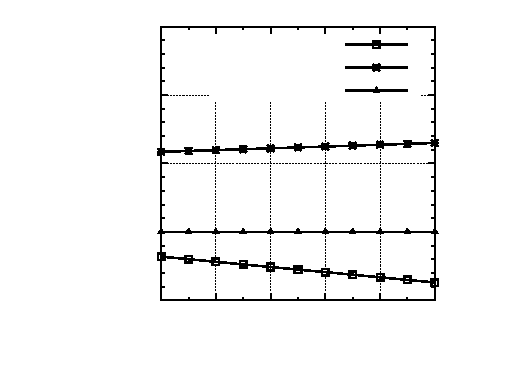
\includegraphics{figures/no2-charge/no2-charge}}%
    \gplfronttext
  \end{picture}%
\endgroup
\\
% GNUPLOT: LaTeX picture with Postscript
\begingroup
  \makeatletter
  \providecommand\color[2][]{%
    \GenericError{(gnuplot) \space\space\space\@spaces}{%
      Package color not loaded in conjunction with
      terminal option `colourtext'%
    }{See the gnuplot documentation for explanation.%
    }{Either use 'blacktext' in gnuplot or load the package
      color.sty in LaTeX.}%
    \renewcommand\color[2][]{}%
  }%
  \providecommand\includegraphics[2][]{%
    \GenericError{(gnuplot) \space\space\space\@spaces}{%
      Package graphicx or graphics not loaded%
    }{See the gnuplot documentation for explanation.%
    }{The gnuplot epslatex terminal needs graphicx.sty or graphics.sty.}%
    \renewcommand\includegraphics[2][]{}%
  }%
  \providecommand\rotatebox[2]{#2}%
  \@ifundefined{ifGPcolor}{%
    \newif\ifGPcolor
    \GPcolortrue
  }{}%
  \@ifundefined{ifGPblacktext}{%
    \newif\ifGPblacktext
    \GPblacktextfalse
  }{}%
  % define a \g@addto@macro without @ in the name:
  \let\gplgaddtomacro\g@addto@macro
  % define empty templates for all commands taking text:
  \gdef\gplbacktext{}%
  \gdef\gplfronttext{}%
  \makeatother
  \ifGPblacktext
    % no textcolor at all
    \def\colorrgb#1{}%
    \def\colorgray#1{}%
  \else
    % gray or color?
    \ifGPcolor
      \def\colorrgb#1{\color[rgb]{#1}}%
      \def\colorgray#1{\color[gray]{#1}}%
      \expandafter\def\csname LTw\endcsname{\color{white}}%
      \expandafter\def\csname LTb\endcsname{\color{black}}%
      \expandafter\def\csname LTa\endcsname{\color{black}}%
      \expandafter\def\csname LT0\endcsname{\color[rgb]{1,0,0}}%
      \expandafter\def\csname LT1\endcsname{\color[rgb]{0,1,0}}%
      \expandafter\def\csname LT2\endcsname{\color[rgb]{0,0,1}}%
      \expandafter\def\csname LT3\endcsname{\color[rgb]{1,0,1}}%
      \expandafter\def\csname LT4\endcsname{\color[rgb]{0,1,1}}%
      \expandafter\def\csname LT5\endcsname{\color[rgb]{1,1,0}}%
      \expandafter\def\csname LT6\endcsname{\color[rgb]{0,0,0}}%
      \expandafter\def\csname LT7\endcsname{\color[rgb]{1,0.3,0}}%
      \expandafter\def\csname LT8\endcsname{\color[rgb]{0.5,0.5,0.5}}%
    \else
      % gray
      \def\colorrgb#1{\color{black}}%
      \def\colorgray#1{\color[gray]{#1}}%
      \expandafter\def\csname LTw\endcsname{\color{white}}%
      \expandafter\def\csname LTb\endcsname{\color{black}}%
      \expandafter\def\csname LTa\endcsname{\color{black}}%
      \expandafter\def\csname LT0\endcsname{\color{black}}%
      \expandafter\def\csname LT1\endcsname{\color{black}}%
      \expandafter\def\csname LT2\endcsname{\color{black}}%
      \expandafter\def\csname LT3\endcsname{\color{black}}%
      \expandafter\def\csname LT4\endcsname{\color{black}}%
      \expandafter\def\csname LT5\endcsname{\color{black}}%
      \expandafter\def\csname LT6\endcsname{\color{black}}%
      \expandafter\def\csname LT7\endcsname{\color{black}}%
      \expandafter\def\csname LT8\endcsname{\color{black}}%
    \fi
  \fi
  \setlength{\unitlength}{0.0500bp}%
  \begin{picture}(5040.00,3772.00)%
    \gplgaddtomacro\gplbacktext{%
      \csname LTb\endcsname%
      \put(1349,880){\makebox(0,0)[r]{\strut{} 0}}%
      \csname LTb\endcsname%
      \put(1349,1537){\makebox(0,0)[r]{\strut{} 5}}%
      \csname LTb\endcsname%
      \put(1349,2194){\makebox(0,0)[r]{\strut{} 10}}%
      \csname LTb\endcsname%
      \put(1349,2850){\makebox(0,0)[r]{\strut{} 15}}%
      \csname LTb\endcsname%
      \put(1349,3507){\makebox(0,0)[r]{\strut{} 20}}%
      \csname LTb\endcsname%
      \put(1481,660){\makebox(0,0){\strut{} 0}}%
      \csname LTb\endcsname%
      \put(2006,660){\makebox(0,0){\strut{} 0.2}}%
      \csname LTb\endcsname%
      \put(2532,660){\makebox(0,0){\strut{} 0.4}}%
      \csname LTb\endcsname%
      \put(3057,660){\makebox(0,0){\strut{} 0.6}}%
      \csname LTb\endcsname%
      \put(3583,660){\makebox(0,0){\strut{} 0.8}}%
      \csname LTb\endcsname%
      \put(4108,660){\makebox(0,0){\strut{} 1}}%
      \put(711,2193){\rotatebox{-270}{\makebox(0,0){\strut{}volume (\AA$^{3}$)}}}%
      \put(2794,330){\makebox(0,0){\strut{}$\lambda$}}%
    }%
    \gplgaddtomacro\gplfronttext{%
      \csname LTb\endcsname%
      \put(3121,3334){\makebox(0,0)[r]{\strut{}C $\rightarrow$ O}}%
      \csname LTb\endcsname%
      \put(3121,3114){\makebox(0,0)[r]{\strut{}C $\rightarrow$ N}}%
      \csname LTb\endcsname%
      \put(3121,2894){\makebox(0,0)[r]{\strut{}H $\rightarrow$ Dummy}}%
    }%
    \gplbacktext
    \put(0,0){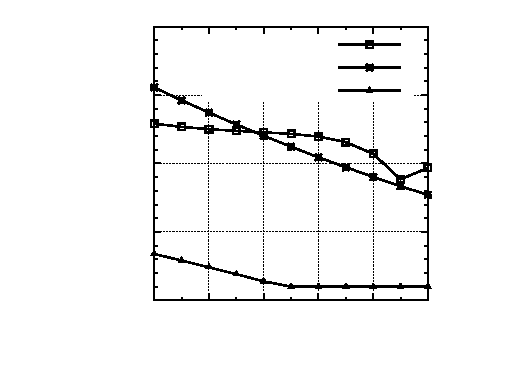
\includegraphics{figures/no2-vol/no2-vol}}%
    \gplfronttext
  \end{picture}%
\endgroup
\hspace*{-1.3cm}% GNUPLOT: LaTeX picture with Postscript
\begingroup
  \makeatletter
  \providecommand\color[2][]{%
    \GenericError{(gnuplot) \space\space\space\@spaces}{%
      Package color not loaded in conjunction with
      terminal option `colourtext'%
    }{See the gnuplot documentation for explanation.%
    }{Either use 'blacktext' in gnuplot or load the package
      color.sty in LaTeX.}%
    \renewcommand\color[2][]{}%
  }%
  \providecommand\includegraphics[2][]{%
    \GenericError{(gnuplot) \space\space\space\@spaces}{%
      Package graphicx or graphics not loaded%
    }{See the gnuplot documentation for explanation.%
    }{The gnuplot epslatex terminal needs graphicx.sty or graphics.sty.}%
    \renewcommand\includegraphics[2][]{}%
  }%
  \providecommand\rotatebox[2]{#2}%
  \@ifundefined{ifGPcolor}{%
    \newif\ifGPcolor
    \GPcolortrue
  }{}%
  \@ifundefined{ifGPblacktext}{%
    \newif\ifGPblacktext
    \GPblacktextfalse
  }{}%
  % define a \g@addto@macro without @ in the name:
  \let\gplgaddtomacro\g@addto@macro
  % define empty templates for all commands taking text:
  \gdef\gplbacktext{}%
  \gdef\gplfronttext{}%
  \makeatother
  \ifGPblacktext
    % no textcolor at all
    \def\colorrgb#1{}%
    \def\colorgray#1{}%
  \else
    % gray or color?
    \ifGPcolor
      \def\colorrgb#1{\color[rgb]{#1}}%
      \def\colorgray#1{\color[gray]{#1}}%
      \expandafter\def\csname LTw\endcsname{\color{white}}%
      \expandafter\def\csname LTb\endcsname{\color{black}}%
      \expandafter\def\csname LTa\endcsname{\color{black}}%
      \expandafter\def\csname LT0\endcsname{\color[rgb]{1,0,0}}%
      \expandafter\def\csname LT1\endcsname{\color[rgb]{0,1,0}}%
      \expandafter\def\csname LT2\endcsname{\color[rgb]{0,0,1}}%
      \expandafter\def\csname LT3\endcsname{\color[rgb]{1,0,1}}%
      \expandafter\def\csname LT4\endcsname{\color[rgb]{0,1,1}}%
      \expandafter\def\csname LT5\endcsname{\color[rgb]{1,1,0}}%
      \expandafter\def\csname LT6\endcsname{\color[rgb]{0,0,0}}%
      \expandafter\def\csname LT7\endcsname{\color[rgb]{1,0.3,0}}%
      \expandafter\def\csname LT8\endcsname{\color[rgb]{0.5,0.5,0.5}}%
    \else
      % gray
      \def\colorrgb#1{\color{black}}%
      \def\colorgray#1{\color[gray]{#1}}%
      \expandafter\def\csname LTw\endcsname{\color{white}}%
      \expandafter\def\csname LTb\endcsname{\color{black}}%
      \expandafter\def\csname LTa\endcsname{\color{black}}%
      \expandafter\def\csname LT0\endcsname{\color{black}}%
      \expandafter\def\csname LT1\endcsname{\color{black}}%
      \expandafter\def\csname LT2\endcsname{\color{black}}%
      \expandafter\def\csname LT3\endcsname{\color{black}}%
      \expandafter\def\csname LT4\endcsname{\color{black}}%
      \expandafter\def\csname LT5\endcsname{\color{black}}%
      \expandafter\def\csname LT6\endcsname{\color{black}}%
      \expandafter\def\csname LT7\endcsname{\color{black}}%
      \expandafter\def\csname LT8\endcsname{\color{black}}%
    \fi
  \fi
  \setlength{\unitlength}{0.0500bp}%
  \begin{picture}(5040.00,3772.00)%
    \gplgaddtomacro\gplbacktext{%
      \csname LTb\endcsname%
      \put(1415,1044){\makebox(0,0)[r]{\strut{}-100}}%
      \csname LTb\endcsname%
      \put(1415,1373){\makebox(0,0)[r]{\strut{}-80}}%
      \csname LTb\endcsname%
      \put(1415,1701){\makebox(0,0)[r]{\strut{}-60}}%
      \csname LTb\endcsname%
      \put(1415,2029){\makebox(0,0)[r]{\strut{}-40}}%
      \csname LTb\endcsname%
      \put(1415,2358){\makebox(0,0)[r]{\strut{}-20}}%
      \csname LTb\endcsname%
      \put(1415,2686){\makebox(0,0)[r]{\strut{} 0}}%
      \csname LTb\endcsname%
      \put(1415,3014){\makebox(0,0)[r]{\strut{} 20}}%
      \csname LTb\endcsname%
      \put(1415,3343){\makebox(0,0)[r]{\strut{} 40}}%
      \csname LTb\endcsname%
      \put(1547,660){\makebox(0,0){\strut{} 0}}%
      \csname LTb\endcsname%
      \put(2072,660){\makebox(0,0){\strut{} 0.2}}%
      \csname LTb\endcsname%
      \put(2598,660){\makebox(0,0){\strut{} 0.4}}%
      \csname LTb\endcsname%
      \put(3123,660){\makebox(0,0){\strut{} 0.6}}%
      \csname LTb\endcsname%
      \put(3649,660){\makebox(0,0){\strut{} 0.8}}%
      \csname LTb\endcsname%
      \put(4174,660){\makebox(0,0){\strut{} 1}}%
      \put(645,2193){\rotatebox{-270}{\makebox(0,0){\strut{}$G^\prime_{\textrm{pol},i}$}}}%
      \put(2860,330){\makebox(0,0){\strut{}$\lambda$}}%
    }%
    \gplgaddtomacro\gplfronttext{%
      \csname LTb\endcsname%
      \put(3187,3334){\makebox(0,0)[r]{\strut{}C $\rightarrow$ O}}%
      \csname LTb\endcsname%
      \put(3187,3114){\makebox(0,0)[r]{\strut{}C $\rightarrow$ N}}%
      \csname LTb\endcsname%
      \put(3187,2894){\makebox(0,0)[r]{\strut{}H $\rightarrow$ Dummy}}%
    }%
    \gplbacktext
    \put(0,0){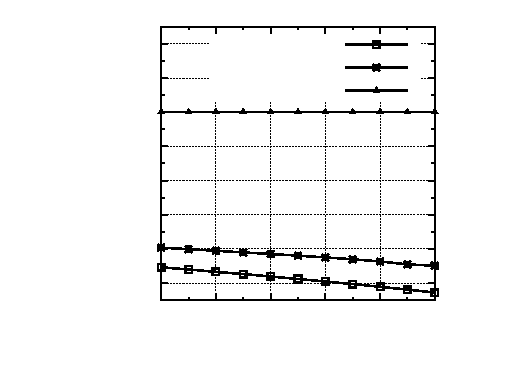
\includegraphics{figures/no2-pol/no2-pol}}%
    \gplfronttext
  \end{picture}%
\endgroup

\caption{The Born energy and components thereof for the perturbation of acetophenone to nitrobenzene. Top left: energy trajectory; top right: charge trajectories; bottom left: volume trajectories; bottom right: electrostatic trajectories.}
\label{no2}
\end{figure}

PhC(O)CH$_3$  $\longrightarrow$ PhNO$_2$. Results for the perturbation of acetophenone to nitrobenzene are given in \cref{no2}. This test case was particularly complicated, featuring three perturbations (methyl carbon to oxygen, $sp^2$ carbon to nitrogen, and hydrogen to dummy) and evolution of a net charge. Further complicating management of charge was perturbation into two N--O atom pairs, a condition that necessitated special accommodation in the FEP GB/SA code. In the event of an N--O group 24\% of the oxygen's charge is added to the nitrogen and removed from the oxygen; in this case, the percent charge added to the nitrogen to each oxygen was scaled on throughout the perturbation, from 0\% at $\lambda = 0$ to 24\% at $\lambda = 1$. Gratifyingly, atomic charges (\cref{no2}, top right) were perturbed linearly throughout the simulation, with the charge on the methyl carbon becoming more negative as it was perturbed to oxygen, the charge on the $sp^2$ carbon becoming more positive as it was perturbed to nitrogen, and the charge on the methyl hydrogens and dummies remaining zero throughout. Volumes (\cref{no2}, bottom left) were predictable with the exception of a small dip in volume for the methyl carbon to oxygen perturbation at $\lambda = 0.9$, although the trajectory was resolved at $\lambda = 1$. Dummy atoms reached the minimum volume of 1.0 \AA$^3$ at $\lambda = 0.5$. Perturbation of electrostatic contribution (\cref{no2}, bottom right) was unremarkable, with contribution from methylene hydrogens to dummy remaining constant at zero. A smooth overall Born energy trajectory arch yielded a modest $\Delta G_{ \textrm{Born}}$ of $+0.15$ kcal/mol for the perturbation. 

These examples highlight the ability of our FEP implementation to handle special cases of charge united-atom to all-atom conversion including expansion/condensation and adjustment, as well as volume overlap, dummy atom and C--H contribution to $G'_{ \textrm{pol},i}$, and geometric perturbations for a wide range of commonly encountered functional groups and functional group transformations.

% ==========================================================================================
% ==========================================================================================
% ==========================================================================================

\subsubsection{Free energies of solvation.}

Having confirmed that the energies and components thereof were well behaved for a wide range of functional group transformations, we were interested in investigating the performance of our implementation if GB/SA with FEP in computing free energies of solvation. Monte Carlo free-energy perturbations were performed for all transformations in Tables \ref{small} and \ref{phxphy} in the gas phase, with GB/SA solvation, and with TIP4P explicit solvation. Standard setup was used in \textit{MCPRO} with 14 windows of doublewide sampling. For the GB/SA and gas-phase calculations, simulations were run for \num{1.66e5} configurations of equilibration followed by \num{5.0e5} configurations of averaging per window, and for the TIP4P calculations, simulations were run for \num{1.0e7} configurations of equilibration followed by \num{3.0e7} configurations of averaging with solute moves attempted every 60 configurations. Using the concept illustrated in the thermodynamic cycle in \cref{thermocycle}, free energies of solvation were then determined. Trajectories of select examples are presented. For each set of trajectories (one set containing GB/SA, TIP4P, and gas phase trajectories), free energies of solvation were determined by evaluating the energy difference between each aqueous trajectory and the gas phase trajectory at their respective endpoints. Whereas only this endpoint was necessary in computing the free energies of solvation, examining the trajectories as a whole gave a sense of the evolution of the energies throughout the perturbation. Remarkably it was demonstrated that the GB/SA simulations yielded not only endpoints similar to those with TIP4P, but in most cases, the energies followed similar trajectories as well, Figures \ref{dgsolphxy1} and \ref{dgsolphxy2}.

\begin{figure}[p]
\centering
% GNUPLOT: LaTeX picture with Postscript
\begingroup
  \makeatletter
  \providecommand\color[2][]{%
    \GenericError{(gnuplot) \space\space\space\@spaces}{%
      Package color not loaded in conjunction with
      terminal option `colourtext'%
    }{See the gnuplot documentation for explanation.%
    }{Either use 'blacktext' in gnuplot or load the package
      color.sty in LaTeX.}%
    \renewcommand\color[2][]{}%
  }%
  \providecommand\includegraphics[2][]{%
    \GenericError{(gnuplot) \space\space\space\@spaces}{%
      Package graphicx or graphics not loaded%
    }{See the gnuplot documentation for explanation.%
    }{The gnuplot epslatex terminal needs graphicx.sty or graphics.sty.}%
    \renewcommand\includegraphics[2][]{}%
  }%
  \providecommand\rotatebox[2]{#2}%
  \@ifundefined{ifGPcolor}{%
    \newif\ifGPcolor
    \GPcolortrue
  }{}%
  \@ifundefined{ifGPblacktext}{%
    \newif\ifGPblacktext
    \GPblacktextfalse
  }{}%
  % define a \g@addto@macro without @ in the name:
  \let\gplgaddtomacro\g@addto@macro
  % define empty templates for all commands taking text:
  \gdef\gplbacktext{}%
  \gdef\gplfronttext{}%
  \makeatother
  \ifGPblacktext
    % no textcolor at all
    \def\colorrgb#1{}%
    \def\colorgray#1{}%
  \else
    % gray or color?
    \ifGPcolor
      \def\colorrgb#1{\color[rgb]{#1}}%
      \def\colorgray#1{\color[gray]{#1}}%
      \expandafter\def\csname LTw\endcsname{\color{white}}%
      \expandafter\def\csname LTb\endcsname{\color{black}}%
      \expandafter\def\csname LTa\endcsname{\color{black}}%
      \expandafter\def\csname LT0\endcsname{\color[rgb]{1,0,0}}%
      \expandafter\def\csname LT1\endcsname{\color[rgb]{0,1,0}}%
      \expandafter\def\csname LT2\endcsname{\color[rgb]{0,0,1}}%
      \expandafter\def\csname LT3\endcsname{\color[rgb]{1,0,1}}%
      \expandafter\def\csname LT4\endcsname{\color[rgb]{0,1,1}}%
      \expandafter\def\csname LT5\endcsname{\color[rgb]{1,1,0}}%
      \expandafter\def\csname LT6\endcsname{\color[rgb]{0,0,0}}%
      \expandafter\def\csname LT7\endcsname{\color[rgb]{1,0.3,0}}%
      \expandafter\def\csname LT8\endcsname{\color[rgb]{0.5,0.5,0.5}}%
    \else
      % gray
      \def\colorrgb#1{\color{black}}%
      \def\colorgray#1{\color[gray]{#1}}%
      \expandafter\def\csname LTw\endcsname{\color{white}}%
      \expandafter\def\csname LTb\endcsname{\color{black}}%
      \expandafter\def\csname LTa\endcsname{\color{black}}%
      \expandafter\def\csname LT0\endcsname{\color{black}}%
      \expandafter\def\csname LT1\endcsname{\color{black}}%
      \expandafter\def\csname LT2\endcsname{\color{black}}%
      \expandafter\def\csname LT3\endcsname{\color{black}}%
      \expandafter\def\csname LT4\endcsname{\color{black}}%
      \expandafter\def\csname LT5\endcsname{\color{black}}%
      \expandafter\def\csname LT6\endcsname{\color{black}}%
      \expandafter\def\csname LT7\endcsname{\color{black}}%
      \expandafter\def\csname LT8\endcsname{\color{black}}%
    \fi
  \fi
  \setlength{\unitlength}{0.0500bp}%
  \begin{picture}(5040.00,3772.00)%
    \gplgaddtomacro\gplbacktext{%
      \csname LTb\endcsname%
      \put(1613,880){\makebox(0,0)[r]{\strut{} 0}}%
      \csname LTb\endcsname%
      \put(1613,1128){\makebox(0,0)[r]{\strut{} 0.2}}%
      \csname LTb\endcsname%
      \put(1613,1376){\makebox(0,0)[r]{\strut{} 0.4}}%
      \csname LTb\endcsname%
      \put(1613,1624){\makebox(0,0)[r]{\strut{} 0.6}}%
      \csname LTb\endcsname%
      \put(1613,1872){\makebox(0,0)[r]{\strut{} 0.8}}%
      \csname LTb\endcsname%
      \put(1613,2119){\makebox(0,0)[r]{\strut{} 1}}%
      \csname LTb\endcsname%
      \put(1613,2367){\makebox(0,0)[r]{\strut{} 1.2}}%
      \csname LTb\endcsname%
      \put(1613,2615){\makebox(0,0)[r]{\strut{} 1.4}}%
      \csname LTb\endcsname%
      \put(1613,2863){\makebox(0,0)[r]{\strut{} 1.6}}%
      \csname LTb\endcsname%
      \put(1613,3111){\makebox(0,0)[r]{\strut{} 1.8}}%
      \csname LTb\endcsname%
      \put(1745,660){\makebox(0,0){\strut{} 0}}%
      \csname LTb\endcsname%
      \put(2191,660){\makebox(0,0){\strut{} 0.2}}%
      \csname LTb\endcsname%
      \put(2637,660){\makebox(0,0){\strut{} 0.4}}%
      \csname LTb\endcsname%
      \put(3084,660){\makebox(0,0){\strut{} 0.6}}%
      \csname LTb\endcsname%
      \put(3530,660){\makebox(0,0){\strut{} 0.8}}%
      \csname LTb\endcsname%
      \put(3976,660){\makebox(0,0){\strut{} 1}}%
      \put(843,1995){\rotatebox{-270}{\makebox(0,0){\strut{}$\Delta G_\textrm{sol}$ (kcal/mol)}}}%
      \put(2860,330){\makebox(0,0){\strut{}$\lambda$}}%
      \put(2860,3441){\makebox(0,0){\strut{}PhCl $\longrightarrow$ PhH}}%
    }%
    \gplgaddtomacro\gplfronttext{%
      \csname LTb\endcsname%
      \put(2989,2938){\makebox(0,0)[r]{\strut{}GB/SA}}%
      \csname LTb\endcsname%
      \put(2989,2718){\makebox(0,0)[r]{\strut{}TIP4P}}%
      \csname LTb\endcsname%
      \put(2989,2498){\makebox(0,0)[r]{\strut{}Gas Phase}}%
    }%
    \gplbacktext
    \put(0,0){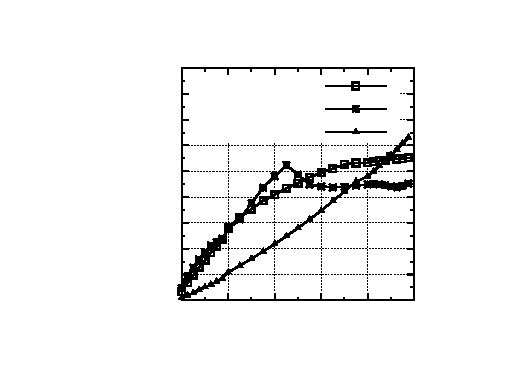
\includegraphics{figures/clh-dgsol/clh-dgsol}}%
    \gplfronttext
  \end{picture}%
\endgroup
\hspace*{-1.3cm}% GNUPLOT: LaTeX picture with Postscript
\begingroup
  \makeatletter
  \providecommand\color[2][]{%
    \GenericError{(gnuplot) \space\space\space\@spaces}{%
      Package color not loaded in conjunction with
      terminal option `colourtext'%
    }{See the gnuplot documentation for explanation.%
    }{Either use 'blacktext' in gnuplot or load the package
      color.sty in LaTeX.}%
    \renewcommand\color[2][]{}%
  }%
  \providecommand\includegraphics[2][]{%
    \GenericError{(gnuplot) \space\space\space\@spaces}{%
      Package graphicx or graphics not loaded%
    }{See the gnuplot documentation for explanation.%
    }{The gnuplot epslatex terminal needs graphicx.sty or graphics.sty.}%
    \renewcommand\includegraphics[2][]{}%
  }%
  \providecommand\rotatebox[2]{#2}%
  \@ifundefined{ifGPcolor}{%
    \newif\ifGPcolor
    \GPcolortrue
  }{}%
  \@ifundefined{ifGPblacktext}{%
    \newif\ifGPblacktext
    \GPblacktextfalse
  }{}%
  % define a \g@addto@macro without @ in the name:
  \let\gplgaddtomacro\g@addto@macro
  % define empty templates for all commands taking text:
  \gdef\gplbacktext{}%
  \gdef\gplfronttext{}%
  \makeatother
  \ifGPblacktext
    % no textcolor at all
    \def\colorrgb#1{}%
    \def\colorgray#1{}%
  \else
    % gray or color?
    \ifGPcolor
      \def\colorrgb#1{\color[rgb]{#1}}%
      \def\colorgray#1{\color[gray]{#1}}%
      \expandafter\def\csname LTw\endcsname{\color{white}}%
      \expandafter\def\csname LTb\endcsname{\color{black}}%
      \expandafter\def\csname LTa\endcsname{\color{black}}%
      \expandafter\def\csname LT0\endcsname{\color[rgb]{1,0,0}}%
      \expandafter\def\csname LT1\endcsname{\color[rgb]{0,1,0}}%
      \expandafter\def\csname LT2\endcsname{\color[rgb]{0,0,1}}%
      \expandafter\def\csname LT3\endcsname{\color[rgb]{1,0,1}}%
      \expandafter\def\csname LT4\endcsname{\color[rgb]{0,1,1}}%
      \expandafter\def\csname LT5\endcsname{\color[rgb]{1,1,0}}%
      \expandafter\def\csname LT6\endcsname{\color[rgb]{0,0,0}}%
      \expandafter\def\csname LT7\endcsname{\color[rgb]{1,0.3,0}}%
      \expandafter\def\csname LT8\endcsname{\color[rgb]{0.5,0.5,0.5}}%
    \else
      % gray
      \def\colorrgb#1{\color{black}}%
      \def\colorgray#1{\color[gray]{#1}}%
      \expandafter\def\csname LTw\endcsname{\color{white}}%
      \expandafter\def\csname LTb\endcsname{\color{black}}%
      \expandafter\def\csname LTa\endcsname{\color{black}}%
      \expandafter\def\csname LT0\endcsname{\color{black}}%
      \expandafter\def\csname LT1\endcsname{\color{black}}%
      \expandafter\def\csname LT2\endcsname{\color{black}}%
      \expandafter\def\csname LT3\endcsname{\color{black}}%
      \expandafter\def\csname LT4\endcsname{\color{black}}%
      \expandafter\def\csname LT5\endcsname{\color{black}}%
      \expandafter\def\csname LT6\endcsname{\color{black}}%
      \expandafter\def\csname LT7\endcsname{\color{black}}%
      \expandafter\def\csname LT8\endcsname{\color{black}}%
    \fi
  \fi
  \setlength{\unitlength}{0.0500bp}%
  \begin{picture}(5040.00,3772.00)%
    \gplgaddtomacro\gplbacktext{%
      \csname LTb\endcsname%
      \put(1481,880){\makebox(0,0)[r]{\strut{}-6}}%
      \csname LTb\endcsname%
      \put(1481,1128){\makebox(0,0)[r]{\strut{}-5}}%
      \csname LTb\endcsname%
      \put(1481,1376){\makebox(0,0)[r]{\strut{}-4}}%
      \csname LTb\endcsname%
      \put(1481,1624){\makebox(0,0)[r]{\strut{}-3}}%
      \csname LTb\endcsname%
      \put(1481,1872){\makebox(0,0)[r]{\strut{}-2}}%
      \csname LTb\endcsname%
      \put(1481,2119){\makebox(0,0)[r]{\strut{}-1}}%
      \csname LTb\endcsname%
      \put(1481,2367){\makebox(0,0)[r]{\strut{} 0}}%
      \csname LTb\endcsname%
      \put(1481,2615){\makebox(0,0)[r]{\strut{} 1}}%
      \csname LTb\endcsname%
      \put(1481,2863){\makebox(0,0)[r]{\strut{} 2}}%
      \csname LTb\endcsname%
      \put(1481,3111){\makebox(0,0)[r]{\strut{} 3}}%
      \csname LTb\endcsname%
      \put(1613,660){\makebox(0,0){\strut{} 0}}%
      \csname LTb\endcsname%
      \put(2059,660){\makebox(0,0){\strut{} 0.2}}%
      \csname LTb\endcsname%
      \put(2505,660){\makebox(0,0){\strut{} 0.4}}%
      \csname LTb\endcsname%
      \put(2952,660){\makebox(0,0){\strut{} 0.6}}%
      \csname LTb\endcsname%
      \put(3398,660){\makebox(0,0){\strut{} 0.8}}%
      \csname LTb\endcsname%
      \put(3844,660){\makebox(0,0){\strut{} 1}}%
      \put(975,1995){\rotatebox{-270}{\makebox(0,0){\strut{}$\Delta G_\textrm{sol}$ (kcal/mol)}}}%
      \put(2728,330){\makebox(0,0){\strut{}$\lambda$}}%
      \put(2728,3441){\makebox(0,0){\strut{}PhCN $\longrightarrow$ PhF}}%
    }%
    \gplgaddtomacro\gplfronttext{%
      \csname LTb\endcsname%
      \put(2857,2938){\makebox(0,0)[r]{\strut{}GB/SA}}%
      \csname LTb\endcsname%
      \put(2857,2718){\makebox(0,0)[r]{\strut{}TIP4P}}%
      \csname LTb\endcsname%
      \put(2857,2498){\makebox(0,0)[r]{\strut{}Gas Phase}}%
    }%
    \gplbacktext
    \put(0,0){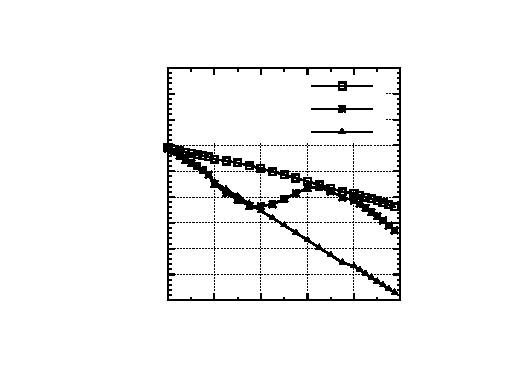
\includegraphics{figures/cnf-dgsol/cnf-dgsol}}%
    \gplfronttext
  \end{picture}%
\endgroup
\\
% GNUPLOT: LaTeX picture with Postscript
\begingroup
  \makeatletter
  \providecommand\color[2][]{%
    \GenericError{(gnuplot) \space\space\space\@spaces}{%
      Package color not loaded in conjunction with
      terminal option `colourtext'%
    }{See the gnuplot documentation for explanation.%
    }{Either use 'blacktext' in gnuplot or load the package
      color.sty in LaTeX.}%
    \renewcommand\color[2][]{}%
  }%
  \providecommand\includegraphics[2][]{%
    \GenericError{(gnuplot) \space\space\space\@spaces}{%
      Package graphicx or graphics not loaded%
    }{See the gnuplot documentation for explanation.%
    }{The gnuplot epslatex terminal needs graphicx.sty or graphics.sty.}%
    \renewcommand\includegraphics[2][]{}%
  }%
  \providecommand\rotatebox[2]{#2}%
  \@ifundefined{ifGPcolor}{%
    \newif\ifGPcolor
    \GPcolortrue
  }{}%
  \@ifundefined{ifGPblacktext}{%
    \newif\ifGPblacktext
    \GPblacktextfalse
  }{}%
  % define a \g@addto@macro without @ in the name:
  \let\gplgaddtomacro\g@addto@macro
  % define empty templates for all commands taking text:
  \gdef\gplbacktext{}%
  \gdef\gplfronttext{}%
  \makeatother
  \ifGPblacktext
    % no textcolor at all
    \def\colorrgb#1{}%
    \def\colorgray#1{}%
  \else
    % gray or color?
    \ifGPcolor
      \def\colorrgb#1{\color[rgb]{#1}}%
      \def\colorgray#1{\color[gray]{#1}}%
      \expandafter\def\csname LTw\endcsname{\color{white}}%
      \expandafter\def\csname LTb\endcsname{\color{black}}%
      \expandafter\def\csname LTa\endcsname{\color{black}}%
      \expandafter\def\csname LT0\endcsname{\color[rgb]{1,0,0}}%
      \expandafter\def\csname LT1\endcsname{\color[rgb]{0,1,0}}%
      \expandafter\def\csname LT2\endcsname{\color[rgb]{0,0,1}}%
      \expandafter\def\csname LT3\endcsname{\color[rgb]{1,0,1}}%
      \expandafter\def\csname LT4\endcsname{\color[rgb]{0,1,1}}%
      \expandafter\def\csname LT5\endcsname{\color[rgb]{1,1,0}}%
      \expandafter\def\csname LT6\endcsname{\color[rgb]{0,0,0}}%
      \expandafter\def\csname LT7\endcsname{\color[rgb]{1,0.3,0}}%
      \expandafter\def\csname LT8\endcsname{\color[rgb]{0.5,0.5,0.5}}%
    \else
      % gray
      \def\colorrgb#1{\color{black}}%
      \def\colorgray#1{\color[gray]{#1}}%
      \expandafter\def\csname LTw\endcsname{\color{white}}%
      \expandafter\def\csname LTb\endcsname{\color{black}}%
      \expandafter\def\csname LTa\endcsname{\color{black}}%
      \expandafter\def\csname LT0\endcsname{\color{black}}%
      \expandafter\def\csname LT1\endcsname{\color{black}}%
      \expandafter\def\csname LT2\endcsname{\color{black}}%
      \expandafter\def\csname LT3\endcsname{\color{black}}%
      \expandafter\def\csname LT4\endcsname{\color{black}}%
      \expandafter\def\csname LT5\endcsname{\color{black}}%
      \expandafter\def\csname LT6\endcsname{\color{black}}%
      \expandafter\def\csname LT7\endcsname{\color{black}}%
      \expandafter\def\csname LT8\endcsname{\color{black}}%
    \fi
  \fi
  \setlength{\unitlength}{0.0500bp}%
  \begin{picture}(5040.00,3772.00)%
    \gplgaddtomacro\gplbacktext{%
      \csname LTb\endcsname%
      \put(1547,1083){\makebox(0,0)[r]{\strut{}-30}}%
      \csname LTb\endcsname%
      \put(1547,1488){\makebox(0,0)[r]{\strut{}-20}}%
      \csname LTb\endcsname%
      \put(1547,1894){\makebox(0,0)[r]{\strut{}-10}}%
      \csname LTb\endcsname%
      \put(1547,2300){\makebox(0,0)[r]{\strut{} 0}}%
      \csname LTb\endcsname%
      \put(1547,2705){\makebox(0,0)[r]{\strut{} 10}}%
      \csname LTb\endcsname%
      \put(1547,3111){\makebox(0,0)[r]{\strut{} 20}}%
      \csname LTb\endcsname%
      \put(1679,660){\makebox(0,0){\strut{} 0}}%
      \csname LTb\endcsname%
      \put(2125,660){\makebox(0,0){\strut{} 0.2}}%
      \csname LTb\endcsname%
      \put(2571,660){\makebox(0,0){\strut{} 0.4}}%
      \csname LTb\endcsname%
      \put(3018,660){\makebox(0,0){\strut{} 0.6}}%
      \csname LTb\endcsname%
      \put(3464,660){\makebox(0,0){\strut{} 0.8}}%
      \csname LTb\endcsname%
      \put(3910,660){\makebox(0,0){\strut{} 1}}%
      \put(909,1995){\rotatebox{-270}{\makebox(0,0){\strut{}$\Delta G_\textrm{sol}$ (kcal/mol)}}}%
      \put(2794,330){\makebox(0,0){\strut{}$\lambda$}}%
      \put(2794,3441){\makebox(0,0){\strut{}PhC(O)CH$_3$ $\longrightarrow$ PhC(O)NH$_2$}}%
    }%
    \gplgaddtomacro\gplfronttext{%
      \csname LTb\endcsname%
      \put(2923,2938){\makebox(0,0)[r]{\strut{}GB/SA}}%
      \csname LTb\endcsname%
      \put(2923,2718){\makebox(0,0)[r]{\strut{}TIP4P}}%
      \csname LTb\endcsname%
      \put(2923,2498){\makebox(0,0)[r]{\strut{}Gas Phase}}%
    }%
    \gplbacktext
    \put(0,0){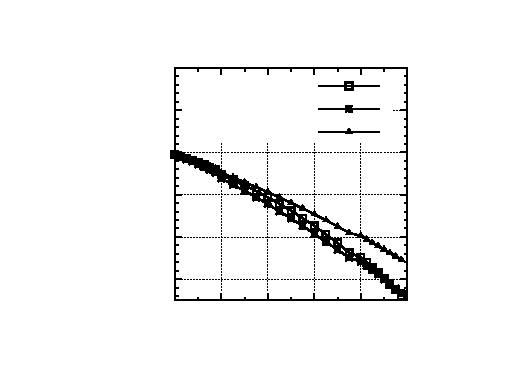
\includegraphics{figures/comenh2-dgsol/comenh2-dgsol}}%
    \gplfronttext
  \end{picture}%
\endgroup
\hspace*{-1.3cm}% GNUPLOT: LaTeX picture with Postscript
\begingroup
  \makeatletter
  \providecommand\color[2][]{%
    \GenericError{(gnuplot) \space\space\space\@spaces}{%
      Package color not loaded in conjunction with
      terminal option `colourtext'%
    }{See the gnuplot documentation for explanation.%
    }{Either use 'blacktext' in gnuplot or load the package
      color.sty in LaTeX.}%
    \renewcommand\color[2][]{}%
  }%
  \providecommand\includegraphics[2][]{%
    \GenericError{(gnuplot) \space\space\space\@spaces}{%
      Package graphicx or graphics not loaded%
    }{See the gnuplot documentation for explanation.%
    }{The gnuplot epslatex terminal needs graphicx.sty or graphics.sty.}%
    \renewcommand\includegraphics[2][]{}%
  }%
  \providecommand\rotatebox[2]{#2}%
  \@ifundefined{ifGPcolor}{%
    \newif\ifGPcolor
    \GPcolortrue
  }{}%
  \@ifundefined{ifGPblacktext}{%
    \newif\ifGPblacktext
    \GPblacktextfalse
  }{}%
  % define a \g@addto@macro without @ in the name:
  \let\gplgaddtomacro\g@addto@macro
  % define empty templates for all commands taking text:
  \gdef\gplbacktext{}%
  \gdef\gplfronttext{}%
  \makeatother
  \ifGPblacktext
    % no textcolor at all
    \def\colorrgb#1{}%
    \def\colorgray#1{}%
  \else
    % gray or color?
    \ifGPcolor
      \def\colorrgb#1{\color[rgb]{#1}}%
      \def\colorgray#1{\color[gray]{#1}}%
      \expandafter\def\csname LTw\endcsname{\color{white}}%
      \expandafter\def\csname LTb\endcsname{\color{black}}%
      \expandafter\def\csname LTa\endcsname{\color{black}}%
      \expandafter\def\csname LT0\endcsname{\color[rgb]{1,0,0}}%
      \expandafter\def\csname LT1\endcsname{\color[rgb]{0,1,0}}%
      \expandafter\def\csname LT2\endcsname{\color[rgb]{0,0,1}}%
      \expandafter\def\csname LT3\endcsname{\color[rgb]{1,0,1}}%
      \expandafter\def\csname LT4\endcsname{\color[rgb]{0,1,1}}%
      \expandafter\def\csname LT5\endcsname{\color[rgb]{1,1,0}}%
      \expandafter\def\csname LT6\endcsname{\color[rgb]{0,0,0}}%
      \expandafter\def\csname LT7\endcsname{\color[rgb]{1,0.3,0}}%
      \expandafter\def\csname LT8\endcsname{\color[rgb]{0.5,0.5,0.5}}%
    \else
      % gray
      \def\colorrgb#1{\color{black}}%
      \def\colorgray#1{\color[gray]{#1}}%
      \expandafter\def\csname LTw\endcsname{\color{white}}%
      \expandafter\def\csname LTb\endcsname{\color{black}}%
      \expandafter\def\csname LTa\endcsname{\color{black}}%
      \expandafter\def\csname LT0\endcsname{\color{black}}%
      \expandafter\def\csname LT1\endcsname{\color{black}}%
      \expandafter\def\csname LT2\endcsname{\color{black}}%
      \expandafter\def\csname LT3\endcsname{\color{black}}%
      \expandafter\def\csname LT4\endcsname{\color{black}}%
      \expandafter\def\csname LT5\endcsname{\color{black}}%
      \expandafter\def\csname LT6\endcsname{\color{black}}%
      \expandafter\def\csname LT7\endcsname{\color{black}}%
      \expandafter\def\csname LT8\endcsname{\color{black}}%
    \fi
  \fi
  \setlength{\unitlength}{0.0500bp}%
  \begin{picture}(5040.00,3772.00)%
    \gplgaddtomacro\gplbacktext{%
      \csname LTb\endcsname%
      \put(1613,880){\makebox(0,0)[r]{\strut{}-2}}%
      \csname LTb\endcsname%
      \put(1613,1159){\makebox(0,0)[r]{\strut{}-1.5}}%
      \csname LTb\endcsname%
      \put(1613,1438){\makebox(0,0)[r]{\strut{}-1}}%
      \csname LTb\endcsname%
      \put(1613,1717){\makebox(0,0)[r]{\strut{}-0.5}}%
      \csname LTb\endcsname%
      \put(1613,1996){\makebox(0,0)[r]{\strut{} 0}}%
      \csname LTb\endcsname%
      \put(1613,2274){\makebox(0,0)[r]{\strut{} 0.5}}%
      \csname LTb\endcsname%
      \put(1613,2553){\makebox(0,0)[r]{\strut{} 1}}%
      \csname LTb\endcsname%
      \put(1613,2832){\makebox(0,0)[r]{\strut{} 1.5}}%
      \csname LTb\endcsname%
      \put(1613,3111){\makebox(0,0)[r]{\strut{} 2}}%
      \csname LTb\endcsname%
      \put(1745,660){\makebox(0,0){\strut{} 0}}%
      \csname LTb\endcsname%
      \put(2191,660){\makebox(0,0){\strut{} 0.2}}%
      \csname LTb\endcsname%
      \put(2637,660){\makebox(0,0){\strut{} 0.4}}%
      \csname LTb\endcsname%
      \put(3084,660){\makebox(0,0){\strut{} 0.6}}%
      \csname LTb\endcsname%
      \put(3530,660){\makebox(0,0){\strut{} 0.8}}%
      \csname LTb\endcsname%
      \put(3976,660){\makebox(0,0){\strut{} 1}}%
      \put(843,1995){\rotatebox{-270}{\makebox(0,0){\strut{}$\Delta G_\textrm{sol}$ (kcal/mol)}}}%
      \put(2860,330){\makebox(0,0){\strut{}$\lambda$}}%
      \put(2860,3441){\makebox(0,0){\strut{}PhPr $\longrightarrow$ BzOCH$_3$}}%
    }%
    \gplgaddtomacro\gplfronttext{%
      \csname LTb\endcsname%
      \put(2989,2938){\makebox(0,0)[r]{\strut{}GB/SA}}%
      \csname LTb\endcsname%
      \put(2989,2718){\makebox(0,0)[r]{\strut{}TIP4P}}%
      \csname LTb\endcsname%
      \put(2989,2498){\makebox(0,0)[r]{\strut{}Gas Phase}}%
    }%
    \gplbacktext
    \put(0,0){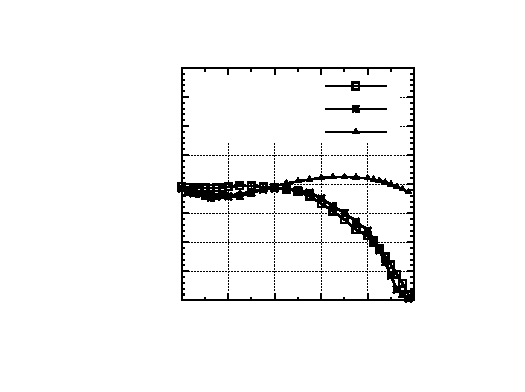
\includegraphics{figures/prmom-dgsol/prmom-dgsol}}%
    \gplfronttext
  \end{picture}%
\endgroup
\\
% GNUPLOT: LaTeX picture with Postscript
\begingroup
  \makeatletter
  \providecommand\color[2][]{%
    \GenericError{(gnuplot) \space\space\space\@spaces}{%
      Package color not loaded in conjunction with
      terminal option `colourtext'%
    }{See the gnuplot documentation for explanation.%
    }{Either use 'blacktext' in gnuplot or load the package
      color.sty in LaTeX.}%
    \renewcommand\color[2][]{}%
  }%
  \providecommand\includegraphics[2][]{%
    \GenericError{(gnuplot) \space\space\space\@spaces}{%
      Package graphicx or graphics not loaded%
    }{See the gnuplot documentation for explanation.%
    }{The gnuplot epslatex terminal needs graphicx.sty or graphics.sty.}%
    \renewcommand\includegraphics[2][]{}%
  }%
  \providecommand\rotatebox[2]{#2}%
  \@ifundefined{ifGPcolor}{%
    \newif\ifGPcolor
    \GPcolortrue
  }{}%
  \@ifundefined{ifGPblacktext}{%
    \newif\ifGPblacktext
    \GPblacktextfalse
  }{}%
  % define a \g@addto@macro without @ in the name:
  \let\gplgaddtomacro\g@addto@macro
  % define empty templates for all commands taking text:
  \gdef\gplbacktext{}%
  \gdef\gplfronttext{}%
  \makeatother
  \ifGPblacktext
    % no textcolor at all
    \def\colorrgb#1{}%
    \def\colorgray#1{}%
  \else
    % gray or color?
    \ifGPcolor
      \def\colorrgb#1{\color[rgb]{#1}}%
      \def\colorgray#1{\color[gray]{#1}}%
      \expandafter\def\csname LTw\endcsname{\color{white}}%
      \expandafter\def\csname LTb\endcsname{\color{black}}%
      \expandafter\def\csname LTa\endcsname{\color{black}}%
      \expandafter\def\csname LT0\endcsname{\color[rgb]{1,0,0}}%
      \expandafter\def\csname LT1\endcsname{\color[rgb]{0,1,0}}%
      \expandafter\def\csname LT2\endcsname{\color[rgb]{0,0,1}}%
      \expandafter\def\csname LT3\endcsname{\color[rgb]{1,0,1}}%
      \expandafter\def\csname LT4\endcsname{\color[rgb]{0,1,1}}%
      \expandafter\def\csname LT5\endcsname{\color[rgb]{1,1,0}}%
      \expandafter\def\csname LT6\endcsname{\color[rgb]{0,0,0}}%
      \expandafter\def\csname LT7\endcsname{\color[rgb]{1,0.3,0}}%
      \expandafter\def\csname LT8\endcsname{\color[rgb]{0.5,0.5,0.5}}%
    \else
      % gray
      \def\colorrgb#1{\color{black}}%
      \def\colorgray#1{\color[gray]{#1}}%
      \expandafter\def\csname LTw\endcsname{\color{white}}%
      \expandafter\def\csname LTb\endcsname{\color{black}}%
      \expandafter\def\csname LTa\endcsname{\color{black}}%
      \expandafter\def\csname LT0\endcsname{\color{black}}%
      \expandafter\def\csname LT1\endcsname{\color{black}}%
      \expandafter\def\csname LT2\endcsname{\color{black}}%
      \expandafter\def\csname LT3\endcsname{\color{black}}%
      \expandafter\def\csname LT4\endcsname{\color{black}}%
      \expandafter\def\csname LT5\endcsname{\color{black}}%
      \expandafter\def\csname LT6\endcsname{\color{black}}%
      \expandafter\def\csname LT7\endcsname{\color{black}}%
      \expandafter\def\csname LT8\endcsname{\color{black}}%
    \fi
  \fi
  \setlength{\unitlength}{0.0500bp}%
  \begin{picture}(5040.00,3772.00)%
    \gplgaddtomacro\gplbacktext{%
      \csname LTb\endcsname%
      \put(1547,880){\makebox(0,0)[r]{\strut{} 0}}%
      \csname LTb\endcsname%
      \put(1547,1159){\makebox(0,0)[r]{\strut{} 2}}%
      \csname LTb\endcsname%
      \put(1547,1438){\makebox(0,0)[r]{\strut{} 4}}%
      \csname LTb\endcsname%
      \put(1547,1717){\makebox(0,0)[r]{\strut{} 6}}%
      \csname LTb\endcsname%
      \put(1547,1996){\makebox(0,0)[r]{\strut{} 8}}%
      \csname LTb\endcsname%
      \put(1547,2274){\makebox(0,0)[r]{\strut{} 10}}%
      \csname LTb\endcsname%
      \put(1547,2553){\makebox(0,0)[r]{\strut{} 12}}%
      \csname LTb\endcsname%
      \put(1547,2832){\makebox(0,0)[r]{\strut{} 14}}%
      \csname LTb\endcsname%
      \put(1547,3111){\makebox(0,0)[r]{\strut{} 16}}%
      \csname LTb\endcsname%
      \put(1679,660){\makebox(0,0){\strut{} 0}}%
      \csname LTb\endcsname%
      \put(2125,660){\makebox(0,0){\strut{} 0.2}}%
      \csname LTb\endcsname%
      \put(2571,660){\makebox(0,0){\strut{} 0.4}}%
      \csname LTb\endcsname%
      \put(3018,660){\makebox(0,0){\strut{} 0.6}}%
      \csname LTb\endcsname%
      \put(3464,660){\makebox(0,0){\strut{} 0.8}}%
      \csname LTb\endcsname%
      \put(3910,660){\makebox(0,0){\strut{} 1}}%
      \put(909,1995){\rotatebox{-270}{\makebox(0,0){\strut{}$\Delta G_\textrm{sol}$ (kcal/mol)}}}%
      \put(2794,330){\makebox(0,0){\strut{}$\lambda$}}%
      \put(2794,3441){\makebox(0,0){\strut{}PhCH$_3$ $\longrightarrow$ PhCF$_3$}}%
    }%
    \gplgaddtomacro\gplfronttext{%
      \csname LTb\endcsname%
      \put(2923,2938){\makebox(0,0)[r]{\strut{}GB/SA}}%
      \csname LTb\endcsname%
      \put(2923,2718){\makebox(0,0)[r]{\strut{}TIP4P}}%
      \csname LTb\endcsname%
      \put(2923,2498){\makebox(0,0)[r]{\strut{}Gas Phase}}%
    }%
    \gplbacktext
    \put(0,0){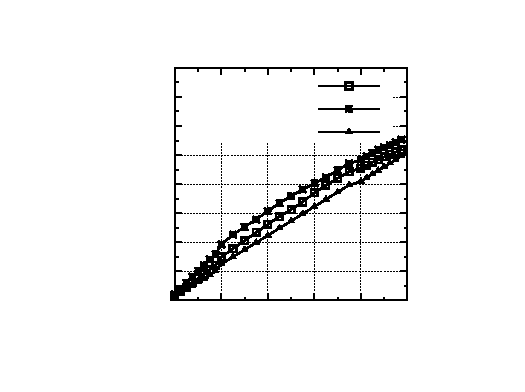
\includegraphics{figures/ch3f3-dgsol/ch3f3-dgsol}}%
    \gplfronttext
  \end{picture}%
\endgroup
\hspace*{-1.3cm}% GNUPLOT: LaTeX picture with Postscript
\begingroup
  \makeatletter
  \providecommand\color[2][]{%
    \GenericError{(gnuplot) \space\space\space\@spaces}{%
      Package color not loaded in conjunction with
      terminal option `colourtext'%
    }{See the gnuplot documentation for explanation.%
    }{Either use 'blacktext' in gnuplot or load the package
      color.sty in LaTeX.}%
    \renewcommand\color[2][]{}%
  }%
  \providecommand\includegraphics[2][]{%
    \GenericError{(gnuplot) \space\space\space\@spaces}{%
      Package graphicx or graphics not loaded%
    }{See the gnuplot documentation for explanation.%
    }{The gnuplot epslatex terminal needs graphicx.sty or graphics.sty.}%
    \renewcommand\includegraphics[2][]{}%
  }%
  \providecommand\rotatebox[2]{#2}%
  \@ifundefined{ifGPcolor}{%
    \newif\ifGPcolor
    \GPcolortrue
  }{}%
  \@ifundefined{ifGPblacktext}{%
    \newif\ifGPblacktext
    \GPblacktextfalse
  }{}%
  % define a \g@addto@macro without @ in the name:
  \let\gplgaddtomacro\g@addto@macro
  % define empty templates for all commands taking text:
  \gdef\gplbacktext{}%
  \gdef\gplfronttext{}%
  \makeatother
  \ifGPblacktext
    % no textcolor at all
    \def\colorrgb#1{}%
    \def\colorgray#1{}%
  \else
    % gray or color?
    \ifGPcolor
      \def\colorrgb#1{\color[rgb]{#1}}%
      \def\colorgray#1{\color[gray]{#1}}%
      \expandafter\def\csname LTw\endcsname{\color{white}}%
      \expandafter\def\csname LTb\endcsname{\color{black}}%
      \expandafter\def\csname LTa\endcsname{\color{black}}%
      \expandafter\def\csname LT0\endcsname{\color[rgb]{1,0,0}}%
      \expandafter\def\csname LT1\endcsname{\color[rgb]{0,1,0}}%
      \expandafter\def\csname LT2\endcsname{\color[rgb]{0,0,1}}%
      \expandafter\def\csname LT3\endcsname{\color[rgb]{1,0,1}}%
      \expandafter\def\csname LT4\endcsname{\color[rgb]{0,1,1}}%
      \expandafter\def\csname LT5\endcsname{\color[rgb]{1,1,0}}%
      \expandafter\def\csname LT6\endcsname{\color[rgb]{0,0,0}}%
      \expandafter\def\csname LT7\endcsname{\color[rgb]{1,0.3,0}}%
      \expandafter\def\csname LT8\endcsname{\color[rgb]{0.5,0.5,0.5}}%
    \else
      % gray
      \def\colorrgb#1{\color{black}}%
      \def\colorgray#1{\color[gray]{#1}}%
      \expandafter\def\csname LTw\endcsname{\color{white}}%
      \expandafter\def\csname LTb\endcsname{\color{black}}%
      \expandafter\def\csname LTa\endcsname{\color{black}}%
      \expandafter\def\csname LT0\endcsname{\color{black}}%
      \expandafter\def\csname LT1\endcsname{\color{black}}%
      \expandafter\def\csname LT2\endcsname{\color{black}}%
      \expandafter\def\csname LT3\endcsname{\color{black}}%
      \expandafter\def\csname LT4\endcsname{\color{black}}%
      \expandafter\def\csname LT5\endcsname{\color{black}}%
      \expandafter\def\csname LT6\endcsname{\color{black}}%
      \expandafter\def\csname LT7\endcsname{\color{black}}%
      \expandafter\def\csname LT8\endcsname{\color{black}}%
    \fi
  \fi
  \setlength{\unitlength}{0.0500bp}%
  \begin{picture}(5040.00,3772.00)%
    \gplgaddtomacro\gplbacktext{%
      \csname LTb\endcsname%
      \put(1547,880){\makebox(0,0)[r]{\strut{} 0}}%
      \csname LTb\endcsname%
      \put(1547,1199){\makebox(0,0)[r]{\strut{} 2}}%
      \csname LTb\endcsname%
      \put(1547,1517){\makebox(0,0)[r]{\strut{} 4}}%
      \csname LTb\endcsname%
      \put(1547,1836){\makebox(0,0)[r]{\strut{} 6}}%
      \csname LTb\endcsname%
      \put(1547,2155){\makebox(0,0)[r]{\strut{} 8}}%
      \csname LTb\endcsname%
      \put(1547,2474){\makebox(0,0)[r]{\strut{} 10}}%
      \csname LTb\endcsname%
      \put(1547,2792){\makebox(0,0)[r]{\strut{} 12}}%
      \csname LTb\endcsname%
      \put(1547,3111){\makebox(0,0)[r]{\strut{} 14}}%
      \csname LTb\endcsname%
      \put(1679,660){\makebox(0,0){\strut{} 0}}%
      \csname LTb\endcsname%
      \put(2125,660){\makebox(0,0){\strut{} 0.2}}%
      \csname LTb\endcsname%
      \put(2571,660){\makebox(0,0){\strut{} 0.4}}%
      \csname LTb\endcsname%
      \put(3018,660){\makebox(0,0){\strut{} 0.6}}%
      \csname LTb\endcsname%
      \put(3464,660){\makebox(0,0){\strut{} 0.8}}%
      \csname LTb\endcsname%
      \put(3910,660){\makebox(0,0){\strut{} 1}}%
      \put(909,1995){\rotatebox{-270}{\makebox(0,0){\strut{}$\Delta G_\textrm{sol}$ (kcal/mol)}}}%
      \put(2794,330){\makebox(0,0){\strut{}$\lambda$}}%
      \put(2794,3441){\makebox(0,0){\strut{}PhC(O)CH$_3$ $\longrightarrow$ PhNO$_2$}}%
    }%
    \gplgaddtomacro\gplfronttext{%
      \csname LTb\endcsname%
      \put(2923,2938){\makebox(0,0)[r]{\strut{}GB/SA}}%
      \csname LTb\endcsname%
      \put(2923,2718){\makebox(0,0)[r]{\strut{}TIP4P}}%
      \csname LTb\endcsname%
      \put(2923,2498){\makebox(0,0)[r]{\strut{}Gas Phase}}%
    }%
    \gplbacktext
    \put(0,0){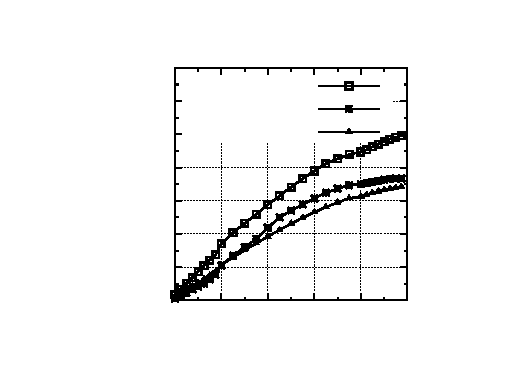
\includegraphics{figures/comeno2-dgsol/comeno2-dgsol}}%
    \gplfronttext
  \end{picture}%
\endgroup
\\
\caption{Selected trajectories for $\Delta G_\textrm{sol}$ from the PhX $\longrightarrow$ PhY (Table \ref{phxphy}) series.}
\label{dgsolphxy1}
\end{figure}

\begin{figure}[p] 
\centering
% GNUPLOT: LaTeX picture with Postscript
\begingroup
  \makeatletter
  \providecommand\color[2][]{%
    \GenericError{(gnuplot) \space\space\space\@spaces}{%
      Package color not loaded in conjunction with
      terminal option `colourtext'%
    }{See the gnuplot documentation for explanation.%
    }{Either use 'blacktext' in gnuplot or load the package
      color.sty in LaTeX.}%
    \renewcommand\color[2][]{}%
  }%
  \providecommand\includegraphics[2][]{%
    \GenericError{(gnuplot) \space\space\space\@spaces}{%
      Package graphicx or graphics not loaded%
    }{See the gnuplot documentation for explanation.%
    }{The gnuplot epslatex terminal needs graphicx.sty or graphics.sty.}%
    \renewcommand\includegraphics[2][]{}%
  }%
  \providecommand\rotatebox[2]{#2}%
  \@ifundefined{ifGPcolor}{%
    \newif\ifGPcolor
    \GPcolortrue
  }{}%
  \@ifundefined{ifGPblacktext}{%
    \newif\ifGPblacktext
    \GPblacktextfalse
  }{}%
  % define a \g@addto@macro without @ in the name:
  \let\gplgaddtomacro\g@addto@macro
  % define empty templates for all commands taking text:
  \gdef\gplbacktext{}%
  \gdef\gplfronttext{}%
  \makeatother
  \ifGPblacktext
    % no textcolor at all
    \def\colorrgb#1{}%
    \def\colorgray#1{}%
  \else
    % gray or color?
    \ifGPcolor
      \def\colorrgb#1{\color[rgb]{#1}}%
      \def\colorgray#1{\color[gray]{#1}}%
      \expandafter\def\csname LTw\endcsname{\color{white}}%
      \expandafter\def\csname LTb\endcsname{\color{black}}%
      \expandafter\def\csname LTa\endcsname{\color{black}}%
      \expandafter\def\csname LT0\endcsname{\color[rgb]{1,0,0}}%
      \expandafter\def\csname LT1\endcsname{\color[rgb]{0,1,0}}%
      \expandafter\def\csname LT2\endcsname{\color[rgb]{0,0,1}}%
      \expandafter\def\csname LT3\endcsname{\color[rgb]{1,0,1}}%
      \expandafter\def\csname LT4\endcsname{\color[rgb]{0,1,1}}%
      \expandafter\def\csname LT5\endcsname{\color[rgb]{1,1,0}}%
      \expandafter\def\csname LT6\endcsname{\color[rgb]{0,0,0}}%
      \expandafter\def\csname LT7\endcsname{\color[rgb]{1,0.3,0}}%
      \expandafter\def\csname LT8\endcsname{\color[rgb]{0.5,0.5,0.5}}%
    \else
      % gray
      \def\colorrgb#1{\color{black}}%
      \def\colorgray#1{\color[gray]{#1}}%
      \expandafter\def\csname LTw\endcsname{\color{white}}%
      \expandafter\def\csname LTb\endcsname{\color{black}}%
      \expandafter\def\csname LTa\endcsname{\color{black}}%
      \expandafter\def\csname LT0\endcsname{\color{black}}%
      \expandafter\def\csname LT1\endcsname{\color{black}}%
      \expandafter\def\csname LT2\endcsname{\color{black}}%
      \expandafter\def\csname LT3\endcsname{\color{black}}%
      \expandafter\def\csname LT4\endcsname{\color{black}}%
      \expandafter\def\csname LT5\endcsname{\color{black}}%
      \expandafter\def\csname LT6\endcsname{\color{black}}%
      \expandafter\def\csname LT7\endcsname{\color{black}}%
      \expandafter\def\csname LT8\endcsname{\color{black}}%
    \fi
  \fi
  \setlength{\unitlength}{0.0500bp}%
  \begin{picture}(5040.00,3772.00)%
    \gplgaddtomacro\gplbacktext{%
      \csname LTb\endcsname%
      \put(1481,880){\makebox(0,0)[r]{\strut{}-8}}%
      \csname LTb\endcsname%
      \put(1481,1252){\makebox(0,0)[r]{\strut{}-6}}%
      \csname LTb\endcsname%
      \put(1481,1624){\makebox(0,0)[r]{\strut{}-4}}%
      \csname LTb\endcsname%
      \put(1481,1996){\makebox(0,0)[r]{\strut{}-2}}%
      \csname LTb\endcsname%
      \put(1481,2367){\makebox(0,0)[r]{\strut{} 0}}%
      \csname LTb\endcsname%
      \put(1481,2739){\makebox(0,0)[r]{\strut{} 2}}%
      \csname LTb\endcsname%
      \put(1481,3111){\makebox(0,0)[r]{\strut{} 4}}%
      \csname LTb\endcsname%
      \put(1613,660){\makebox(0,0){\strut{} 0}}%
      \csname LTb\endcsname%
      \put(2059,660){\makebox(0,0){\strut{} 0.2}}%
      \csname LTb\endcsname%
      \put(2505,660){\makebox(0,0){\strut{} 0.4}}%
      \csname LTb\endcsname%
      \put(2952,660){\makebox(0,0){\strut{} 0.6}}%
      \csname LTb\endcsname%
      \put(3398,660){\makebox(0,0){\strut{} 0.8}}%
      \csname LTb\endcsname%
      \put(3844,660){\makebox(0,0){\strut{} 1}}%
      \put(975,1995){\rotatebox{-270}{\makebox(0,0){\strut{}$\Delta G_\textrm{sol}$ (kcal/mol)}}}%
      \put(2728,330){\makebox(0,0){\strut{}$\lambda$}}%
      \put(2728,3441){\makebox(0,0){\strut{}PhSH $\longrightarrow$ PhOH}}%
    }%
    \gplgaddtomacro\gplfronttext{%
      \csname LTb\endcsname%
      \put(2857,2938){\makebox(0,0)[r]{\strut{}GB/SA}}%
      \csname LTb\endcsname%
      \put(2857,2718){\makebox(0,0)[r]{\strut{}TIP4P}}%
      \csname LTb\endcsname%
      \put(2857,2498){\makebox(0,0)[r]{\strut{}Gas Phase}}%
    }%
    \gplbacktext
    \put(0,0){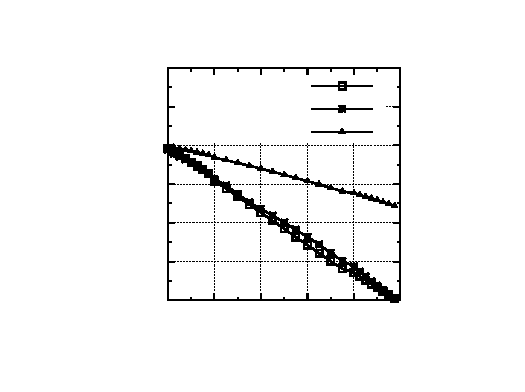
\includegraphics{figures/shoh-dgsol/shoh-dgsol}}%
    \gplfronttext
  \end{picture}%
\endgroup
\hspace*{-1.3cm}% GNUPLOT: LaTeX picture with Postscript
\begingroup
  \makeatletter
  \providecommand\color[2][]{%
    \GenericError{(gnuplot) \space\space\space\@spaces}{%
      Package color not loaded in conjunction with
      terminal option `colourtext'%
    }{See the gnuplot documentation for explanation.%
    }{Either use 'blacktext' in gnuplot or load the package
      color.sty in LaTeX.}%
    \renewcommand\color[2][]{}%
  }%
  \providecommand\includegraphics[2][]{%
    \GenericError{(gnuplot) \space\space\space\@spaces}{%
      Package graphicx or graphics not loaded%
    }{See the gnuplot documentation for explanation.%
    }{The gnuplot epslatex terminal needs graphicx.sty or graphics.sty.}%
    \renewcommand\includegraphics[2][]{}%
  }%
  \providecommand\rotatebox[2]{#2}%
  \@ifundefined{ifGPcolor}{%
    \newif\ifGPcolor
    \GPcolortrue
  }{}%
  \@ifundefined{ifGPblacktext}{%
    \newif\ifGPblacktext
    \GPblacktextfalse
  }{}%
  % define a \g@addto@macro without @ in the name:
  \let\gplgaddtomacro\g@addto@macro
  % define empty templates for all commands taking text:
  \gdef\gplbacktext{}%
  \gdef\gplfronttext{}%
  \makeatother
  \ifGPblacktext
    % no textcolor at all
    \def\colorrgb#1{}%
    \def\colorgray#1{}%
  \else
    % gray or color?
    \ifGPcolor
      \def\colorrgb#1{\color[rgb]{#1}}%
      \def\colorgray#1{\color[gray]{#1}}%
      \expandafter\def\csname LTw\endcsname{\color{white}}%
      \expandafter\def\csname LTb\endcsname{\color{black}}%
      \expandafter\def\csname LTa\endcsname{\color{black}}%
      \expandafter\def\csname LT0\endcsname{\color[rgb]{1,0,0}}%
      \expandafter\def\csname LT1\endcsname{\color[rgb]{0,1,0}}%
      \expandafter\def\csname LT2\endcsname{\color[rgb]{0,0,1}}%
      \expandafter\def\csname LT3\endcsname{\color[rgb]{1,0,1}}%
      \expandafter\def\csname LT4\endcsname{\color[rgb]{0,1,1}}%
      \expandafter\def\csname LT5\endcsname{\color[rgb]{1,1,0}}%
      \expandafter\def\csname LT6\endcsname{\color[rgb]{0,0,0}}%
      \expandafter\def\csname LT7\endcsname{\color[rgb]{1,0.3,0}}%
      \expandafter\def\csname LT8\endcsname{\color[rgb]{0.5,0.5,0.5}}%
    \else
      % gray
      \def\colorrgb#1{\color{black}}%
      \def\colorgray#1{\color[gray]{#1}}%
      \expandafter\def\csname LTw\endcsname{\color{white}}%
      \expandafter\def\csname LTb\endcsname{\color{black}}%
      \expandafter\def\csname LTa\endcsname{\color{black}}%
      \expandafter\def\csname LT0\endcsname{\color{black}}%
      \expandafter\def\csname LT1\endcsname{\color{black}}%
      \expandafter\def\csname LT2\endcsname{\color{black}}%
      \expandafter\def\csname LT3\endcsname{\color{black}}%
      \expandafter\def\csname LT4\endcsname{\color{black}}%
      \expandafter\def\csname LT5\endcsname{\color{black}}%
      \expandafter\def\csname LT6\endcsname{\color{black}}%
      \expandafter\def\csname LT7\endcsname{\color{black}}%
      \expandafter\def\csname LT8\endcsname{\color{black}}%
    \fi
  \fi
  \setlength{\unitlength}{0.0500bp}%
  \begin{picture}(5040.00,3772.00)%
    \gplgaddtomacro\gplbacktext{%
      \csname LTb\endcsname%
      \put(1481,880){\makebox(0,0)[r]{\strut{} 0}}%
      \csname LTb\endcsname%
      \put(1481,1159){\makebox(0,0)[r]{\strut{} 1}}%
      \csname LTb\endcsname%
      \put(1481,1438){\makebox(0,0)[r]{\strut{} 2}}%
      \csname LTb\endcsname%
      \put(1481,1717){\makebox(0,0)[r]{\strut{} 3}}%
      \csname LTb\endcsname%
      \put(1481,1996){\makebox(0,0)[r]{\strut{} 4}}%
      \csname LTb\endcsname%
      \put(1481,2274){\makebox(0,0)[r]{\strut{} 5}}%
      \csname LTb\endcsname%
      \put(1481,2553){\makebox(0,0)[r]{\strut{} 6}}%
      \csname LTb\endcsname%
      \put(1481,2832){\makebox(0,0)[r]{\strut{} 7}}%
      \csname LTb\endcsname%
      \put(1481,3111){\makebox(0,0)[r]{\strut{} 8}}%
      \csname LTb\endcsname%
      \put(1613,660){\makebox(0,0){\strut{} 0}}%
      \csname LTb\endcsname%
      \put(2059,660){\makebox(0,0){\strut{} 0.2}}%
      \csname LTb\endcsname%
      \put(2505,660){\makebox(0,0){\strut{} 0.4}}%
      \csname LTb\endcsname%
      \put(2952,660){\makebox(0,0){\strut{} 0.6}}%
      \csname LTb\endcsname%
      \put(3398,660){\makebox(0,0){\strut{} 0.8}}%
      \csname LTb\endcsname%
      \put(3844,660){\makebox(0,0){\strut{} 1}}%
      \put(975,1995){\rotatebox{-270}{\makebox(0,0){\strut{}$\Delta G_\textrm{sol}$ (kcal/mol)}}}%
      \put(2728,330){\makebox(0,0){\strut{}$\lambda$}}%
      \put(2728,3441){\makebox(0,0){\strut{}PhSCH$_3$ $\longrightarrow$ PhOCH$_3$}}%
    }%
    \gplgaddtomacro\gplfronttext{%
      \csname LTb\endcsname%
      \put(2857,2938){\makebox(0,0)[r]{\strut{}GB/SA}}%
      \csname LTb\endcsname%
      \put(2857,2718){\makebox(0,0)[r]{\strut{}TIP4P}}%
      \csname LTb\endcsname%
      \put(2857,2498){\makebox(0,0)[r]{\strut{}Gas Phase}}%
    }%
    \gplbacktext
    \put(0,0){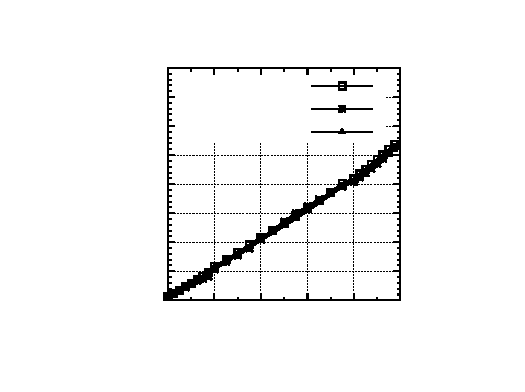
\includegraphics{figures/smeome-dgsol/smeome-dgsol}}%
    \gplfronttext
  \end{picture}%
\endgroup
\\
% GNUPLOT: LaTeX picture with Postscript
\begingroup
  \makeatletter
  \providecommand\color[2][]{%
    \GenericError{(gnuplot) \space\space\space\@spaces}{%
      Package color not loaded in conjunction with
      terminal option `colourtext'%
    }{See the gnuplot documentation for explanation.%
    }{Either use 'blacktext' in gnuplot or load the package
      color.sty in LaTeX.}%
    \renewcommand\color[2][]{}%
  }%
  \providecommand\includegraphics[2][]{%
    \GenericError{(gnuplot) \space\space\space\@spaces}{%
      Package graphicx or graphics not loaded%
    }{See the gnuplot documentation for explanation.%
    }{The gnuplot epslatex terminal needs graphicx.sty or graphics.sty.}%
    \renewcommand\includegraphics[2][]{}%
  }%
  \providecommand\rotatebox[2]{#2}%
  \@ifundefined{ifGPcolor}{%
    \newif\ifGPcolor
    \GPcolortrue
  }{}%
  \@ifundefined{ifGPblacktext}{%
    \newif\ifGPblacktext
    \GPblacktextfalse
  }{}%
  % define a \g@addto@macro without @ in the name:
  \let\gplgaddtomacro\g@addto@macro
  % define empty templates for all commands taking text:
  \gdef\gplbacktext{}%
  \gdef\gplfronttext{}%
  \makeatother
  \ifGPblacktext
    % no textcolor at all
    \def\colorrgb#1{}%
    \def\colorgray#1{}%
  \else
    % gray or color?
    \ifGPcolor
      \def\colorrgb#1{\color[rgb]{#1}}%
      \def\colorgray#1{\color[gray]{#1}}%
      \expandafter\def\csname LTw\endcsname{\color{white}}%
      \expandafter\def\csname LTb\endcsname{\color{black}}%
      \expandafter\def\csname LTa\endcsname{\color{black}}%
      \expandafter\def\csname LT0\endcsname{\color[rgb]{1,0,0}}%
      \expandafter\def\csname LT1\endcsname{\color[rgb]{0,1,0}}%
      \expandafter\def\csname LT2\endcsname{\color[rgb]{0,0,1}}%
      \expandafter\def\csname LT3\endcsname{\color[rgb]{1,0,1}}%
      \expandafter\def\csname LT4\endcsname{\color[rgb]{0,1,1}}%
      \expandafter\def\csname LT5\endcsname{\color[rgb]{1,1,0}}%
      \expandafter\def\csname LT6\endcsname{\color[rgb]{0,0,0}}%
      \expandafter\def\csname LT7\endcsname{\color[rgb]{1,0.3,0}}%
      \expandafter\def\csname LT8\endcsname{\color[rgb]{0.5,0.5,0.5}}%
    \else
      % gray
      \def\colorrgb#1{\color{black}}%
      \def\colorgray#1{\color[gray]{#1}}%
      \expandafter\def\csname LTw\endcsname{\color{white}}%
      \expandafter\def\csname LTb\endcsname{\color{black}}%
      \expandafter\def\csname LTa\endcsname{\color{black}}%
      \expandafter\def\csname LT0\endcsname{\color{black}}%
      \expandafter\def\csname LT1\endcsname{\color{black}}%
      \expandafter\def\csname LT2\endcsname{\color{black}}%
      \expandafter\def\csname LT3\endcsname{\color{black}}%
      \expandafter\def\csname LT4\endcsname{\color{black}}%
      \expandafter\def\csname LT5\endcsname{\color{black}}%
      \expandafter\def\csname LT6\endcsname{\color{black}}%
      \expandafter\def\csname LT7\endcsname{\color{black}}%
      \expandafter\def\csname LT8\endcsname{\color{black}}%
    \fi
  \fi
  \setlength{\unitlength}{0.0500bp}%
  \begin{picture}(5040.00,3772.00)%
    \gplgaddtomacro\gplbacktext{%
      \csname LTb\endcsname%
      \put(1547,880){\makebox(0,0)[r]{\strut{} 0}}%
      \csname LTb\endcsname%
      \put(1547,1199){\makebox(0,0)[r]{\strut{} 2}}%
      \csname LTb\endcsname%
      \put(1547,1517){\makebox(0,0)[r]{\strut{} 4}}%
      \csname LTb\endcsname%
      \put(1547,1836){\makebox(0,0)[r]{\strut{} 6}}%
      \csname LTb\endcsname%
      \put(1547,2155){\makebox(0,0)[r]{\strut{} 8}}%
      \csname LTb\endcsname%
      \put(1547,2474){\makebox(0,0)[r]{\strut{} 10}}%
      \csname LTb\endcsname%
      \put(1547,2792){\makebox(0,0)[r]{\strut{} 12}}%
      \csname LTb\endcsname%
      \put(1547,3111){\makebox(0,0)[r]{\strut{} 14}}%
      \csname LTb\endcsname%
      \put(1679,660){\makebox(0,0){\strut{} 0}}%
      \csname LTb\endcsname%
      \put(2125,660){\makebox(0,0){\strut{} 0.2}}%
      \csname LTb\endcsname%
      \put(2571,660){\makebox(0,0){\strut{} 0.4}}%
      \csname LTb\endcsname%
      \put(3018,660){\makebox(0,0){\strut{} 0.6}}%
      \csname LTb\endcsname%
      \put(3464,660){\makebox(0,0){\strut{} 0.8}}%
      \csname LTb\endcsname%
      \put(3910,660){\makebox(0,0){\strut{} 1}}%
      \put(909,1995){\rotatebox{-270}{\makebox(0,0){\strut{}$\Delta G_\textrm{sol}$ (kcal/mol)}}}%
      \put(2794,330){\makebox(0,0){\strut{}$\lambda$}}%
      \put(2794,3441){\makebox(0,0){\strut{}PhOH $\longrightarrow$ PhF}}%
    }%
    \gplgaddtomacro\gplfronttext{%
      \csname LTb\endcsname%
      \put(2923,2938){\makebox(0,0)[r]{\strut{}GB/SA}}%
      \csname LTb\endcsname%
      \put(2923,2718){\makebox(0,0)[r]{\strut{}TIP4P}}%
      \csname LTb\endcsname%
      \put(2923,2498){\makebox(0,0)[r]{\strut{}Gas Phase}}%
    }%
    \gplbacktext
    \put(0,0){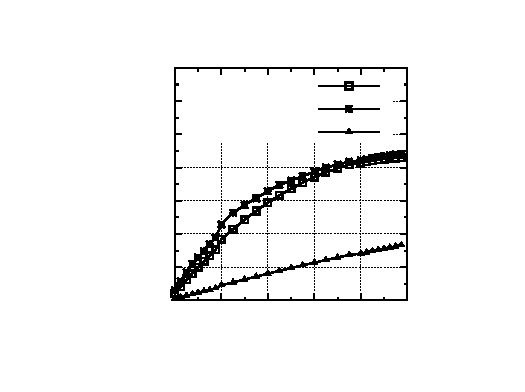
\includegraphics{figures/ohf-dgsol/ohf-dgsol}}%
    \gplfronttext
  \end{picture}%
\endgroup
\hspace*{-1.3cm}% GNUPLOT: LaTeX picture with Postscript
\begingroup
  \makeatletter
  \providecommand\color[2][]{%
    \GenericError{(gnuplot) \space\space\space\@spaces}{%
      Package color not loaded in conjunction with
      terminal option `colourtext'%
    }{See the gnuplot documentation for explanation.%
    }{Either use 'blacktext' in gnuplot or load the package
      color.sty in LaTeX.}%
    \renewcommand\color[2][]{}%
  }%
  \providecommand\includegraphics[2][]{%
    \GenericError{(gnuplot) \space\space\space\@spaces}{%
      Package graphicx or graphics not loaded%
    }{See the gnuplot documentation for explanation.%
    }{The gnuplot epslatex terminal needs graphicx.sty or graphics.sty.}%
    \renewcommand\includegraphics[2][]{}%
  }%
  \providecommand\rotatebox[2]{#2}%
  \@ifundefined{ifGPcolor}{%
    \newif\ifGPcolor
    \GPcolortrue
  }{}%
  \@ifundefined{ifGPblacktext}{%
    \newif\ifGPblacktext
    \GPblacktextfalse
  }{}%
  % define a \g@addto@macro without @ in the name:
  \let\gplgaddtomacro\g@addto@macro
  % define empty templates for all commands taking text:
  \gdef\gplbacktext{}%
  \gdef\gplfronttext{}%
  \makeatother
  \ifGPblacktext
    % no textcolor at all
    \def\colorrgb#1{}%
    \def\colorgray#1{}%
  \else
    % gray or color?
    \ifGPcolor
      \def\colorrgb#1{\color[rgb]{#1}}%
      \def\colorgray#1{\color[gray]{#1}}%
      \expandafter\def\csname LTw\endcsname{\color{white}}%
      \expandafter\def\csname LTb\endcsname{\color{black}}%
      \expandafter\def\csname LTa\endcsname{\color{black}}%
      \expandafter\def\csname LT0\endcsname{\color[rgb]{1,0,0}}%
      \expandafter\def\csname LT1\endcsname{\color[rgb]{0,1,0}}%
      \expandafter\def\csname LT2\endcsname{\color[rgb]{0,0,1}}%
      \expandafter\def\csname LT3\endcsname{\color[rgb]{1,0,1}}%
      \expandafter\def\csname LT4\endcsname{\color[rgb]{0,1,1}}%
      \expandafter\def\csname LT5\endcsname{\color[rgb]{1,1,0}}%
      \expandafter\def\csname LT6\endcsname{\color[rgb]{0,0,0}}%
      \expandafter\def\csname LT7\endcsname{\color[rgb]{1,0.3,0}}%
      \expandafter\def\csname LT8\endcsname{\color[rgb]{0.5,0.5,0.5}}%
    \else
      % gray
      \def\colorrgb#1{\color{black}}%
      \def\colorgray#1{\color[gray]{#1}}%
      \expandafter\def\csname LTw\endcsname{\color{white}}%
      \expandafter\def\csname LTb\endcsname{\color{black}}%
      \expandafter\def\csname LTa\endcsname{\color{black}}%
      \expandafter\def\csname LT0\endcsname{\color{black}}%
      \expandafter\def\csname LT1\endcsname{\color{black}}%
      \expandafter\def\csname LT2\endcsname{\color{black}}%
      \expandafter\def\csname LT3\endcsname{\color{black}}%
      \expandafter\def\csname LT4\endcsname{\color{black}}%
      \expandafter\def\csname LT5\endcsname{\color{black}}%
      \expandafter\def\csname LT6\endcsname{\color{black}}%
      \expandafter\def\csname LT7\endcsname{\color{black}}%
      \expandafter\def\csname LT8\endcsname{\color{black}}%
    \fi
  \fi
  \setlength{\unitlength}{0.0500bp}%
  \begin{picture}(5040.00,3772.00)%
    \gplgaddtomacro\gplbacktext{%
      \csname LTb\endcsname%
      \put(1613,880){\makebox(0,0)[r]{\strut{} 0}}%
      \csname LTb\endcsname%
      \put(1613,1159){\makebox(0,0)[r]{\strut{} 0.5}}%
      \csname LTb\endcsname%
      \put(1613,1438){\makebox(0,0)[r]{\strut{} 1}}%
      \csname LTb\endcsname%
      \put(1613,1717){\makebox(0,0)[r]{\strut{} 1.5}}%
      \csname LTb\endcsname%
      \put(1613,1996){\makebox(0,0)[r]{\strut{} 2}}%
      \csname LTb\endcsname%
      \put(1613,2274){\makebox(0,0)[r]{\strut{} 2.5}}%
      \csname LTb\endcsname%
      \put(1613,2553){\makebox(0,0)[r]{\strut{} 3}}%
      \csname LTb\endcsname%
      \put(1613,2832){\makebox(0,0)[r]{\strut{} 3.5}}%
      \csname LTb\endcsname%
      \put(1613,3111){\makebox(0,0)[r]{\strut{} 4}}%
      \csname LTb\endcsname%
      \put(1745,660){\makebox(0,0){\strut{} 0}}%
      \csname LTb\endcsname%
      \put(2191,660){\makebox(0,0){\strut{} 0.2}}%
      \csname LTb\endcsname%
      \put(2637,660){\makebox(0,0){\strut{} 0.4}}%
      \csname LTb\endcsname%
      \put(3084,660){\makebox(0,0){\strut{} 0.6}}%
      \csname LTb\endcsname%
      \put(3530,660){\makebox(0,0){\strut{} 0.8}}%
      \csname LTb\endcsname%
      \put(3976,660){\makebox(0,0){\strut{} 1}}%
      \put(843,1995){\rotatebox{-270}{\makebox(0,0){\strut{}$\Delta G_\textrm{sol}$ (kcal/mol)}}}%
      \put(2860,330){\makebox(0,0){\strut{}$\lambda$}}%
      \put(2860,3441){\makebox(0,0){\strut{}PhEt $\longrightarrow$ PhOCH$_3$}}%
    }%
    \gplgaddtomacro\gplfronttext{%
      \csname LTb\endcsname%
      \put(2989,2938){\makebox(0,0)[r]{\strut{}GB/SA}}%
      \csname LTb\endcsname%
      \put(2989,2718){\makebox(0,0)[r]{\strut{}TIP4P}}%
      \csname LTb\endcsname%
      \put(2989,2498){\makebox(0,0)[r]{\strut{}Gas Phase}}%
    }%
    \gplbacktext
    \put(0,0){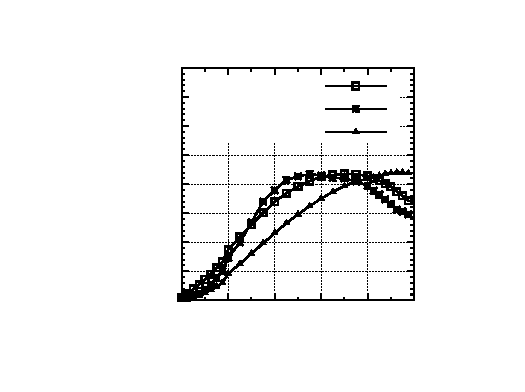
\includegraphics{figures/etome-dgsol/etome-dgsol}}%
    \gplfronttext
  \end{picture}%
\endgroup
\\
% GNUPLOT: LaTeX picture with Postscript
\begingroup
  \makeatletter
  \providecommand\color[2][]{%
    \GenericError{(gnuplot) \space\space\space\@spaces}{%
      Package color not loaded in conjunction with
      terminal option `colourtext'%
    }{See the gnuplot documentation for explanation.%
    }{Either use 'blacktext' in gnuplot or load the package
      color.sty in LaTeX.}%
    \renewcommand\color[2][]{}%
  }%
  \providecommand\includegraphics[2][]{%
    \GenericError{(gnuplot) \space\space\space\@spaces}{%
      Package graphicx or graphics not loaded%
    }{See the gnuplot documentation for explanation.%
    }{The gnuplot epslatex terminal needs graphicx.sty or graphics.sty.}%
    \renewcommand\includegraphics[2][]{}%
  }%
  \providecommand\rotatebox[2]{#2}%
  \@ifundefined{ifGPcolor}{%
    \newif\ifGPcolor
    \GPcolortrue
  }{}%
  \@ifundefined{ifGPblacktext}{%
    \newif\ifGPblacktext
    \GPblacktextfalse
  }{}%
  % define a \g@addto@macro without @ in the name:
  \let\gplgaddtomacro\g@addto@macro
  % define empty templates for all commands taking text:
  \gdef\gplbacktext{}%
  \gdef\gplfronttext{}%
  \makeatother
  \ifGPblacktext
    % no textcolor at all
    \def\colorrgb#1{}%
    \def\colorgray#1{}%
  \else
    % gray or color?
    \ifGPcolor
      \def\colorrgb#1{\color[rgb]{#1}}%
      \def\colorgray#1{\color[gray]{#1}}%
      \expandafter\def\csname LTw\endcsname{\color{white}}%
      \expandafter\def\csname LTb\endcsname{\color{black}}%
      \expandafter\def\csname LTa\endcsname{\color{black}}%
      \expandafter\def\csname LT0\endcsname{\color[rgb]{1,0,0}}%
      \expandafter\def\csname LT1\endcsname{\color[rgb]{0,1,0}}%
      \expandafter\def\csname LT2\endcsname{\color[rgb]{0,0,1}}%
      \expandafter\def\csname LT3\endcsname{\color[rgb]{1,0,1}}%
      \expandafter\def\csname LT4\endcsname{\color[rgb]{0,1,1}}%
      \expandafter\def\csname LT5\endcsname{\color[rgb]{1,1,0}}%
      \expandafter\def\csname LT6\endcsname{\color[rgb]{0,0,0}}%
      \expandafter\def\csname LT7\endcsname{\color[rgb]{1,0.3,0}}%
      \expandafter\def\csname LT8\endcsname{\color[rgb]{0.5,0.5,0.5}}%
    \else
      % gray
      \def\colorrgb#1{\color{black}}%
      \def\colorgray#1{\color[gray]{#1}}%
      \expandafter\def\csname LTw\endcsname{\color{white}}%
      \expandafter\def\csname LTb\endcsname{\color{black}}%
      \expandafter\def\csname LTa\endcsname{\color{black}}%
      \expandafter\def\csname LT0\endcsname{\color{black}}%
      \expandafter\def\csname LT1\endcsname{\color{black}}%
      \expandafter\def\csname LT2\endcsname{\color{black}}%
      \expandafter\def\csname LT3\endcsname{\color{black}}%
      \expandafter\def\csname LT4\endcsname{\color{black}}%
      \expandafter\def\csname LT5\endcsname{\color{black}}%
      \expandafter\def\csname LT6\endcsname{\color{black}}%
      \expandafter\def\csname LT7\endcsname{\color{black}}%
      \expandafter\def\csname LT8\endcsname{\color{black}}%
    \fi
  \fi
  \setlength{\unitlength}{0.0500bp}%
  \begin{picture}(5040.00,3772.00)%
    \gplgaddtomacro\gplbacktext{%
      \csname LTb\endcsname%
      \put(1547,880){\makebox(0,0)[r]{\strut{} 0}}%
      \csname LTb\endcsname%
      \put(1547,1159){\makebox(0,0)[r]{\strut{} 2}}%
      \csname LTb\endcsname%
      \put(1547,1438){\makebox(0,0)[r]{\strut{} 4}}%
      \csname LTb\endcsname%
      \put(1547,1717){\makebox(0,0)[r]{\strut{} 6}}%
      \csname LTb\endcsname%
      \put(1547,1996){\makebox(0,0)[r]{\strut{} 8}}%
      \csname LTb\endcsname%
      \put(1547,2274){\makebox(0,0)[r]{\strut{} 10}}%
      \csname LTb\endcsname%
      \put(1547,2553){\makebox(0,0)[r]{\strut{} 12}}%
      \csname LTb\endcsname%
      \put(1547,2832){\makebox(0,0)[r]{\strut{} 14}}%
      \csname LTb\endcsname%
      \put(1547,3111){\makebox(0,0)[r]{\strut{} 16}}%
      \csname LTb\endcsname%
      \put(1679,660){\makebox(0,0){\strut{} 0}}%
      \csname LTb\endcsname%
      \put(2125,660){\makebox(0,0){\strut{} 0.2}}%
      \csname LTb\endcsname%
      \put(2571,660){\makebox(0,0){\strut{} 0.4}}%
      \csname LTb\endcsname%
      \put(3018,660){\makebox(0,0){\strut{} 0.6}}%
      \csname LTb\endcsname%
      \put(3464,660){\makebox(0,0){\strut{} 0.8}}%
      \csname LTb\endcsname%
      \put(3910,660){\makebox(0,0){\strut{} 1}}%
      \put(909,1995){\rotatebox{-270}{\makebox(0,0){\strut{}$\Delta G_\textrm{sol}$ (kcal/mol)}}}%
      \put(2794,330){\makebox(0,0){\strut{}$\lambda$}}%
      \put(2794,3441){\makebox(0,0){\strut{}PhOH $\longrightarrow$ PhOCH$_3$}}%
    }%
    \gplgaddtomacro\gplfronttext{%
      \csname LTb\endcsname%
      \put(2923,2938){\makebox(0,0)[r]{\strut{}GB/SA}}%
      \csname LTb\endcsname%
      \put(2923,2718){\makebox(0,0)[r]{\strut{}TIP4P}}%
      \csname LTb\endcsname%
      \put(2923,2498){\makebox(0,0)[r]{\strut{}Gas Phase}}%
    }%
    \gplbacktext
    \put(0,0){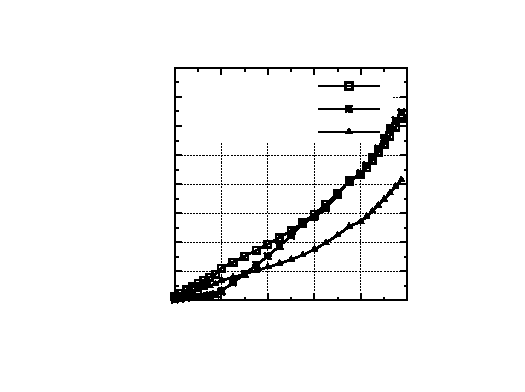
\includegraphics{figures/ohome-dgsol/ohome-dgsol}}%
    \gplfronttext
  \end{picture}%
\endgroup
\hspace*{-1.3cm}% GNUPLOT: LaTeX picture with Postscript
\begingroup
  \makeatletter
  \providecommand\color[2][]{%
    \GenericError{(gnuplot) \space\space\space\@spaces}{%
      Package color not loaded in conjunction with
      terminal option `colourtext'%
    }{See the gnuplot documentation for explanation.%
    }{Either use 'blacktext' in gnuplot or load the package
      color.sty in LaTeX.}%
    \renewcommand\color[2][]{}%
  }%
  \providecommand\includegraphics[2][]{%
    \GenericError{(gnuplot) \space\space\space\@spaces}{%
      Package graphicx or graphics not loaded%
    }{See the gnuplot documentation for explanation.%
    }{The gnuplot epslatex terminal needs graphicx.sty or graphics.sty.}%
    \renewcommand\includegraphics[2][]{}%
  }%
  \providecommand\rotatebox[2]{#2}%
  \@ifundefined{ifGPcolor}{%
    \newif\ifGPcolor
    \GPcolortrue
  }{}%
  \@ifundefined{ifGPblacktext}{%
    \newif\ifGPblacktext
    \GPblacktextfalse
  }{}%
  % define a \g@addto@macro without @ in the name:
  \let\gplgaddtomacro\g@addto@macro
  % define empty templates for all commands taking text:
  \gdef\gplbacktext{}%
  \gdef\gplfronttext{}%
  \makeatother
  \ifGPblacktext
    % no textcolor at all
    \def\colorrgb#1{}%
    \def\colorgray#1{}%
  \else
    % gray or color?
    \ifGPcolor
      \def\colorrgb#1{\color[rgb]{#1}}%
      \def\colorgray#1{\color[gray]{#1}}%
      \expandafter\def\csname LTw\endcsname{\color{white}}%
      \expandafter\def\csname LTb\endcsname{\color{black}}%
      \expandafter\def\csname LTa\endcsname{\color{black}}%
      \expandafter\def\csname LT0\endcsname{\color[rgb]{1,0,0}}%
      \expandafter\def\csname LT1\endcsname{\color[rgb]{0,1,0}}%
      \expandafter\def\csname LT2\endcsname{\color[rgb]{0,0,1}}%
      \expandafter\def\csname LT3\endcsname{\color[rgb]{1,0,1}}%
      \expandafter\def\csname LT4\endcsname{\color[rgb]{0,1,1}}%
      \expandafter\def\csname LT5\endcsname{\color[rgb]{1,1,0}}%
      \expandafter\def\csname LT6\endcsname{\color[rgb]{0,0,0}}%
      \expandafter\def\csname LT7\endcsname{\color[rgb]{1,0.3,0}}%
      \expandafter\def\csname LT8\endcsname{\color[rgb]{0.5,0.5,0.5}}%
    \else
      % gray
      \def\colorrgb#1{\color{black}}%
      \def\colorgray#1{\color[gray]{#1}}%
      \expandafter\def\csname LTw\endcsname{\color{white}}%
      \expandafter\def\csname LTb\endcsname{\color{black}}%
      \expandafter\def\csname LTa\endcsname{\color{black}}%
      \expandafter\def\csname LT0\endcsname{\color{black}}%
      \expandafter\def\csname LT1\endcsname{\color{black}}%
      \expandafter\def\csname LT2\endcsname{\color{black}}%
      \expandafter\def\csname LT3\endcsname{\color{black}}%
      \expandafter\def\csname LT4\endcsname{\color{black}}%
      \expandafter\def\csname LT5\endcsname{\color{black}}%
      \expandafter\def\csname LT6\endcsname{\color{black}}%
      \expandafter\def\csname LT7\endcsname{\color{black}}%
      \expandafter\def\csname LT8\endcsname{\color{black}}%
    \fi
  \fi
  \setlength{\unitlength}{0.0500bp}%
  \begin{picture}(5040.00,3772.00)%
    \gplgaddtomacro\gplbacktext{%
      \csname LTb\endcsname%
      \put(1547,880){\makebox(0,0)[r]{\strut{}-14}}%
      \csname LTb\endcsname%
      \put(1547,1128){\makebox(0,0)[r]{\strut{}-12}}%
      \csname LTb\endcsname%
      \put(1547,1376){\makebox(0,0)[r]{\strut{}-10}}%
      \csname LTb\endcsname%
      \put(1547,1624){\makebox(0,0)[r]{\strut{}-8}}%
      \csname LTb\endcsname%
      \put(1547,1872){\makebox(0,0)[r]{\strut{}-6}}%
      \csname LTb\endcsname%
      \put(1547,2119){\makebox(0,0)[r]{\strut{}-4}}%
      \csname LTb\endcsname%
      \put(1547,2367){\makebox(0,0)[r]{\strut{}-2}}%
      \csname LTb\endcsname%
      \put(1547,2615){\makebox(0,0)[r]{\strut{} 0}}%
      \csname LTb\endcsname%
      \put(1547,2863){\makebox(0,0)[r]{\strut{} 2}}%
      \csname LTb\endcsname%
      \put(1547,3111){\makebox(0,0)[r]{\strut{} 4}}%
      \csname LTb\endcsname%
      \put(1679,660){\makebox(0,0){\strut{} 0}}%
      \csname LTb\endcsname%
      \put(2125,660){\makebox(0,0){\strut{} 0.2}}%
      \csname LTb\endcsname%
      \put(2571,660){\makebox(0,0){\strut{} 0.4}}%
      \csname LTb\endcsname%
      \put(3018,660){\makebox(0,0){\strut{} 0.6}}%
      \csname LTb\endcsname%
      \put(3464,660){\makebox(0,0){\strut{} 0.8}}%
      \csname LTb\endcsname%
      \put(3910,660){\makebox(0,0){\strut{} 1}}%
      \put(909,1995){\rotatebox{-270}{\makebox(0,0){\strut{}$\Delta G_\textrm{sol}$ (kcal/mol)}}}%
      \put(2794,330){\makebox(0,0){\strut{}$\lambda$}}%
      \put(2794,3441){\makebox(0,0){\strut{}PhOCH$_3$ $\longrightarrow$ PhOH}}%
    }%
    \gplgaddtomacro\gplfronttext{%
      \csname LTb\endcsname%
      \put(2923,2938){\makebox(0,0)[r]{\strut{}GB/SA}}%
      \csname LTb\endcsname%
      \put(2923,2718){\makebox(0,0)[r]{\strut{}TIP4P}}%
      \csname LTb\endcsname%
      \put(2923,2498){\makebox(0,0)[r]{\strut{}Gas Phase}}%
    }%
    \gplbacktext
    \put(0,0){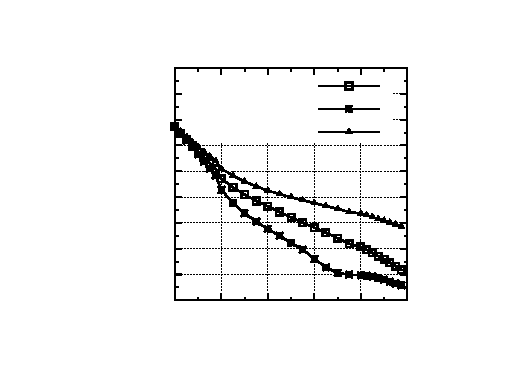
\includegraphics{figures/omeoh-dgsol/omeoh-dgsol}}%
    \gplfronttext
  \end{picture}%
\endgroup
\\
\caption{More selected trajectories for $\Delta G_\textrm{sol}$ from the PhX $\longrightarrow$ PhY (Table \ref{phxphy}) series.}
\label{dgsolphxy2}
\end{figure}

\begin{figure}[t!]
\centering
% GNUPLOT: LaTeX picture with Postscript
\begingroup
  \makeatletter
  \providecommand\color[2][]{%
    \GenericError{(gnuplot) \space\space\space\@spaces}{%
      Package color not loaded in conjunction with
      terminal option `colourtext'%
    }{See the gnuplot documentation for explanation.%
    }{Either use 'blacktext' in gnuplot or load the package
      color.sty in LaTeX.}%
    \renewcommand\color[2][]{}%
  }%
  \providecommand\includegraphics[2][]{%
    \GenericError{(gnuplot) \space\space\space\@spaces}{%
      Package graphicx or graphics not loaded%
    }{See the gnuplot documentation for explanation.%
    }{The gnuplot epslatex terminal needs graphicx.sty or graphics.sty.}%
    \renewcommand\includegraphics[2][]{}%
  }%
  \providecommand\rotatebox[2]{#2}%
  \@ifundefined{ifGPcolor}{%
    \newif\ifGPcolor
    \GPcolortrue
  }{}%
  \@ifundefined{ifGPblacktext}{%
    \newif\ifGPblacktext
    \GPblacktextfalse
  }{}%
  % define a \g@addto@macro without @ in the name:
  \let\gplgaddtomacro\g@addto@macro
  % define empty templates for all commands taking text:
  \gdef\gplbacktext{}%
  \gdef\gplfronttext{}%
  \makeatother
  \ifGPblacktext
    % no textcolor at all
    \def\colorrgb#1{}%
    \def\colorgray#1{}%
  \else
    % gray or color?
    \ifGPcolor
      \def\colorrgb#1{\color[rgb]{#1}}%
      \def\colorgray#1{\color[gray]{#1}}%
      \expandafter\def\csname LTw\endcsname{\color{white}}%
      \expandafter\def\csname LTb\endcsname{\color{black}}%
      \expandafter\def\csname LTa\endcsname{\color{black}}%
      \expandafter\def\csname LT0\endcsname{\color[rgb]{1,0,0}}%
      \expandafter\def\csname LT1\endcsname{\color[rgb]{0,1,0}}%
      \expandafter\def\csname LT2\endcsname{\color[rgb]{0,0,1}}%
      \expandafter\def\csname LT3\endcsname{\color[rgb]{1,0,1}}%
      \expandafter\def\csname LT4\endcsname{\color[rgb]{0,1,1}}%
      \expandafter\def\csname LT5\endcsname{\color[rgb]{1,1,0}}%
      \expandafter\def\csname LT6\endcsname{\color[rgb]{0,0,0}}%
      \expandafter\def\csname LT7\endcsname{\color[rgb]{1,0.3,0}}%
      \expandafter\def\csname LT8\endcsname{\color[rgb]{0.5,0.5,0.5}}%
    \else
      % gray
      \def\colorrgb#1{\color{black}}%
      \def\colorgray#1{\color[gray]{#1}}%
      \expandafter\def\csname LTw\endcsname{\color{white}}%
      \expandafter\def\csname LTb\endcsname{\color{black}}%
      \expandafter\def\csname LTa\endcsname{\color{black}}%
      \expandafter\def\csname LT0\endcsname{\color{black}}%
      \expandafter\def\csname LT1\endcsname{\color{black}}%
      \expandafter\def\csname LT2\endcsname{\color{black}}%
      \expandafter\def\csname LT3\endcsname{\color{black}}%
      \expandafter\def\csname LT4\endcsname{\color{black}}%
      \expandafter\def\csname LT5\endcsname{\color{black}}%
      \expandafter\def\csname LT6\endcsname{\color{black}}%
      \expandafter\def\csname LT7\endcsname{\color{black}}%
      \expandafter\def\csname LT8\endcsname{\color{black}}%
    \fi
  \fi
  \setlength{\unitlength}{0.0500bp}%
  \begin{picture}(7200.00,5040.00)%
    \gplgaddtomacro\gplbacktext{%
      \csname LTb\endcsname%
      \put(814,880){\makebox(0,0)[r]{\strut{}-10}}%
      \csname LTb\endcsname%
      \put(814,1313){\makebox(0,0)[r]{\strut{}-8}}%
      \csname LTb\endcsname%
      \put(814,1746){\makebox(0,0)[r]{\strut{}-6}}%
      \csname LTb\endcsname%
      \put(814,2178){\makebox(0,0)[r]{\strut{}-4}}%
      \csname LTb\endcsname%
      \put(814,2611){\makebox(0,0)[r]{\strut{}-2}}%
      \csname LTb\endcsname%
      \put(814,3044){\makebox(0,0)[r]{\strut{} 0}}%
      \csname LTb\endcsname%
      \put(814,3477){\makebox(0,0)[r]{\strut{} 2}}%
      \csname LTb\endcsname%
      \put(814,3909){\makebox(0,0)[r]{\strut{} 4}}%
      \csname LTb\endcsname%
      \put(814,4342){\makebox(0,0)[r]{\strut{} 6}}%
      \csname LTb\endcsname%
      \put(814,4775){\makebox(0,0)[r]{\strut{} 8}}%
      \csname LTb\endcsname%
      \put(946,660){\makebox(0,0){\strut{}-10}}%
      \csname LTb\endcsname%
      \put(1678,660){\makebox(0,0){\strut{}-8}}%
      \csname LTb\endcsname%
      \put(2410,660){\makebox(0,0){\strut{}-6}}%
      \csname LTb\endcsname%
      \put(3142,660){\makebox(0,0){\strut{}-4}}%
      \csname LTb\endcsname%
      \put(3875,660){\makebox(0,0){\strut{}-2}}%
      \csname LTb\endcsname%
      \put(4607,660){\makebox(0,0){\strut{} 0}}%
      \csname LTb\endcsname%
      \put(5339,660){\makebox(0,0){\strut{} 2}}%
      \csname LTb\endcsname%
      \put(6071,660){\makebox(0,0){\strut{} 4}}%
      \csname LTb\endcsname%
      \put(6803,660){\makebox(0,0){\strut{} 6}}%
      \put(250,2827){\rotatebox{-270}{\makebox(0,0){\strut{}$\Delta\Delta G_\textrm{sol}$(GB/SA)}}}%
      \put(3874,330){\makebox(0,0){\strut{}$\Delta\Delta G_\textrm{sol}$(TIP4P)}}%
    }%
    \gplgaddtomacro\gplfronttext{%
      \csname LTb\endcsname%
      \put(5816,4602){\makebox(0,0)[r]{\strut{}fit: $y = 0.9708x + 0.7141$}}%
    }%
    \gplbacktext
    \put(0,0){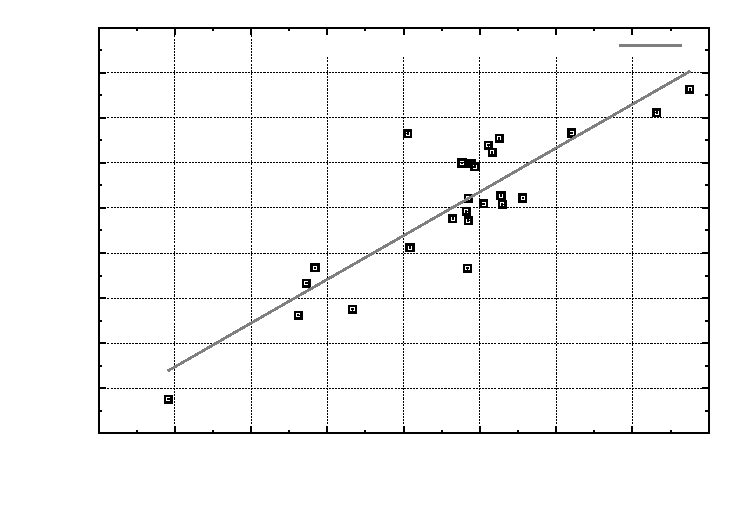
\includegraphics{figures/corrphxy/corrphxy}}%
    \gplfronttext
  \end{picture}%
\endgroup

\caption{Correlation plot between GB/SA and TIP4P for the entire PhX $\longrightarrow$ PhY test set, $r^2$ = 0.7588, $y = 0.9708x + 0.7141$.}
\label{corrphxy}
\end{figure}

For the perturbation of 
chlorobenzene to benzene, 
$\Delta G_{\textrm{GB/SA}}(\textrm{\textbf{A}}\longrightarrow\textrm{\textbf{B}})$ = 1.104 kcal/mol, 
$\Delta G_{\textrm{TIP4P}}(\textrm{\textbf{A}}\longrightarrow\textrm{\textbf{B}})$ = 0.904 kcal/mol, and 
$\Delta G_{\textrm{gas}}(\textrm{\textbf{A}}\longrightarrow\textrm{\textbf{B}})$ = 1.261 kcal/mol. 
Thus, relative free energies of solvation for the perturbation of chlorobenzene to benzene were $-0.157$ kcal/mol for GB/SA and $-0.357$ kcal/mol for TIP4P. For the PhX $\longrightarrow$  PhY set in general, GB/SA trajectories behaved more like gas-phase trajectories than TIP4P trajectories; GB/SA and gas-phase trajectories typically followed a more predictable path, whereas TIP4P trajectories often fluctuated, owing to variations in water molecule configurations. 
Such examples are given by 
chlorobenzene to benzene, 
cyanobenzene to fluorobenzene 
$(\Delta\Delta G_{ \textrm{sol}}(\textrm{GB/SA})$ = 3.325 kcal/mol, 
$\Delta\Delta G_{ \textrm{sol}}(\textrm{TIP4P})$ = 2.408 kcal/mol), 
ethylbenzene to anisole 
$(\Delta\Delta G_{ \textrm{sol}}(\textrm{GB/SA})$ = $-0.501$ kcal/mol, 
$\Delta\Delta G_{ \textrm{sol}}(\textrm{TIP4P})$ = 0.717 kcal/mol), as well as 
anisole to phenol 
$(\Delta\Delta G_{ \textrm{sol}}(\textrm{GB/SA})$ = $-3.335$ kcal/mol, 
$\Delta\Delta G_{ \textrm{sol}}(\textrm{TIP4P})$ = $-4.549$ kcal/mol). 
Fortunately, most deviations were small and eventually corrected themselves. Additionally, there were many cases where the GB/SA and TIP4P trajectories mimicked each other's, illustrated by perturbations of 
acetophenone to benzamide 
$(\Delta\Delta G_{ \textrm{sol}}(\textrm{GB/SA})$ = $-8.480$ kcal/mol, 
$\Delta\Delta G_{ \textrm{sol}}(\textrm{TIP4P})$ = $-7.865$ kcal/mol), 
propylbenzene to benzyl methyl ether 
$(\Delta\Delta G_{ \textrm{sol}}(\textrm{GB/SA})$ = $-1.765$ kcal/mol, 
$\Delta\Delta G_{ \textrm{sol}}(\textrm{TIP4P})$ = $-1.833$ kcal/mol), 
thiophenol to phenol 
$(\Delta\Delta G_{ \textrm{sol}}(\textrm{GB/SA})$ = $-4.758$ kcal/mol, 
$\Delta\Delta G_{ \textrm{sol}}(\textrm{TIP4P})$ = $-4.764$ kcal/mol), 
thioanisole to anisole 
$(\Delta\Delta G_{ \textrm{sol}}(\textrm{GB/SA})$ = 0.182 kcal/mol, 
$\Delta\Delta G_{ \textrm{sol}}(\textrm{TIP4P})$ = 0.102 kcal/mol), 
as well as phenol to fluorobenzene 
$(\Delta\Delta G_{ \textrm{sol}}(\textrm{GB/SA})$ = 5.261 kcal/mol, 
$\Delta\Delta G_{ \textrm{sol}}(\textrm{TIP4P})$ = 5.506 kcal/mol), 
and ethylbenzene to anisole 
$(\Delta\Delta G_{ \textrm{sol}}(\textrm{GB/SA})$ = $-0.477$ kcal/mol, 
$\Delta\Delta G_{ \textrm{sol}}(\textrm{TIP4P})$ = $0.710$ kcal/mol) and 
phenol to anisole 
$(\Delta\Delta G_{ \textrm{sol}}(\textrm{GB/SA})$ = 4.227 kcal/mol, 
$\Delta\Delta G_{ \textrm{sol}}(\textrm{TIP4P})$ = 4.640 kcal/mol). 
One example of a perturbation run forwards and backwards is given for phenol to anisole and anisole to phenol. 
Hysteresis was larger for GB/SA (forwards 
$\Delta\Delta G_{ \textrm{sol}}(\textrm{GB/SA})$ = 4.227 kcal/mol, backwards 
$\Delta\Delta G_{ \textrm{sol}}(\textrm{GB/SA})$ = $-3.335$ kcal/mol, 
hysteresis = 0.892 kcal/mol) 
than for TIP4P (forwards 
$\Delta\Delta G_{ \textrm{sol}}(\textrm{TIP4P})$ = 4.640 kcal/mol, backwards 
$\Delta\Delta G_{ \textrm{sol}}(\textrm{TIP4P})$ = $-4.549$ kcal/mol, 
hysteresis = 0.091 kcal/mol). 
Overall, GB/SA performed reasonably well in reproducing relative free energies of solvation in TIP4P explicit water (\cref{corrphxy}) with a correlation value $r^{2} = 0.7588$. 

\begin{figure}[p]
\centering
% GNUPLOT: LaTeX picture with Postscript
\begingroup
  \makeatletter
  \providecommand\color[2][]{%
    \GenericError{(gnuplot) \space\space\space\@spaces}{%
      Package color not loaded in conjunction with
      terminal option `colourtext'%
    }{See the gnuplot documentation for explanation.%
    }{Either use 'blacktext' in gnuplot or load the package
      color.sty in LaTeX.}%
    \renewcommand\color[2][]{}%
  }%
  \providecommand\includegraphics[2][]{%
    \GenericError{(gnuplot) \space\space\space\@spaces}{%
      Package graphicx or graphics not loaded%
    }{See the gnuplot documentation for explanation.%
    }{The gnuplot epslatex terminal needs graphicx.sty or graphics.sty.}%
    \renewcommand\includegraphics[2][]{}%
  }%
  \providecommand\rotatebox[2]{#2}%
  \@ifundefined{ifGPcolor}{%
    \newif\ifGPcolor
    \GPcolortrue
  }{}%
  \@ifundefined{ifGPblacktext}{%
    \newif\ifGPblacktext
    \GPblacktextfalse
  }{}%
  % define a \g@addto@macro without @ in the name:
  \let\gplgaddtomacro\g@addto@macro
  % define empty templates for all commands taking text:
  \gdef\gplbacktext{}%
  \gdef\gplfronttext{}%
  \makeatother
  \ifGPblacktext
    % no textcolor at all
    \def\colorrgb#1{}%
    \def\colorgray#1{}%
  \else
    % gray or color?
    \ifGPcolor
      \def\colorrgb#1{\color[rgb]{#1}}%
      \def\colorgray#1{\color[gray]{#1}}%
      \expandafter\def\csname LTw\endcsname{\color{white}}%
      \expandafter\def\csname LTb\endcsname{\color{black}}%
      \expandafter\def\csname LTa\endcsname{\color{black}}%
      \expandafter\def\csname LT0\endcsname{\color[rgb]{1,0,0}}%
      \expandafter\def\csname LT1\endcsname{\color[rgb]{0,1,0}}%
      \expandafter\def\csname LT2\endcsname{\color[rgb]{0,0,1}}%
      \expandafter\def\csname LT3\endcsname{\color[rgb]{1,0,1}}%
      \expandafter\def\csname LT4\endcsname{\color[rgb]{0,1,1}}%
      \expandafter\def\csname LT5\endcsname{\color[rgb]{1,1,0}}%
      \expandafter\def\csname LT6\endcsname{\color[rgb]{0,0,0}}%
      \expandafter\def\csname LT7\endcsname{\color[rgb]{1,0.3,0}}%
      \expandafter\def\csname LT8\endcsname{\color[rgb]{0.5,0.5,0.5}}%
    \else
      % gray
      \def\colorrgb#1{\color{black}}%
      \def\colorgray#1{\color[gray]{#1}}%
      \expandafter\def\csname LTw\endcsname{\color{white}}%
      \expandafter\def\csname LTb\endcsname{\color{black}}%
      \expandafter\def\csname LTa\endcsname{\color{black}}%
      \expandafter\def\csname LT0\endcsname{\color{black}}%
      \expandafter\def\csname LT1\endcsname{\color{black}}%
      \expandafter\def\csname LT2\endcsname{\color{black}}%
      \expandafter\def\csname LT3\endcsname{\color{black}}%
      \expandafter\def\csname LT4\endcsname{\color{black}}%
      \expandafter\def\csname LT5\endcsname{\color{black}}%
      \expandafter\def\csname LT6\endcsname{\color{black}}%
      \expandafter\def\csname LT7\endcsname{\color{black}}%
      \expandafter\def\csname LT8\endcsname{\color{black}}%
    \fi
  \fi
  \setlength{\unitlength}{0.0500bp}%
  \begin{picture}(5040.00,3772.00)%
    \gplgaddtomacro\gplbacktext{%
      \csname LTb\endcsname%
      \put(1481,880){\makebox(0,0)[r]{\strut{}-3}}%
      \csname LTb\endcsname%
      \put(1481,1252){\makebox(0,0)[r]{\strut{}-2}}%
      \csname LTb\endcsname%
      \put(1481,1624){\makebox(0,0)[r]{\strut{}-1}}%
      \csname LTb\endcsname%
      \put(1481,1996){\makebox(0,0)[r]{\strut{} 0}}%
      \csname LTb\endcsname%
      \put(1481,2367){\makebox(0,0)[r]{\strut{} 1}}%
      \csname LTb\endcsname%
      \put(1481,2739){\makebox(0,0)[r]{\strut{} 2}}%
      \csname LTb\endcsname%
      \put(1481,3111){\makebox(0,0)[r]{\strut{} 3}}%
      \csname LTb\endcsname%
      \put(1613,660){\makebox(0,0){\strut{} 0}}%
      \csname LTb\endcsname%
      \put(2059,660){\makebox(0,0){\strut{} 0.2}}%
      \csname LTb\endcsname%
      \put(2505,660){\makebox(0,0){\strut{} 0.4}}%
      \csname LTb\endcsname%
      \put(2952,660){\makebox(0,0){\strut{} 0.6}}%
      \csname LTb\endcsname%
      \put(3398,660){\makebox(0,0){\strut{} 0.8}}%
      \csname LTb\endcsname%
      \put(3844,660){\makebox(0,0){\strut{} 1}}%
      \put(975,1995){\rotatebox{-270}{\makebox(0,0){\strut{}$\Delta G_\textrm{sol}$ (kcal/mol)}}}%
      \put(2728,330){\makebox(0,0){\strut{}$\lambda$}}%
      \put(2728,3441){\makebox(0,0){\strut{}H$_3$C---CH$_3$ $\longrightarrow$ H$_3$C---H}}%
    }%
    \gplgaddtomacro\gplfronttext{%
      \csname LTb\endcsname%
      \put(2857,2938){\makebox(0,0)[r]{\strut{}GB/SA}}%
      \csname LTb\endcsname%
      \put(2857,2718){\makebox(0,0)[r]{\strut{}TIP4P}}%
      \csname LTb\endcsname%
      \put(2857,2498){\makebox(0,0)[r]{\strut{}Gas Phase}}%
    }%
    \gplbacktext
    \put(0,0){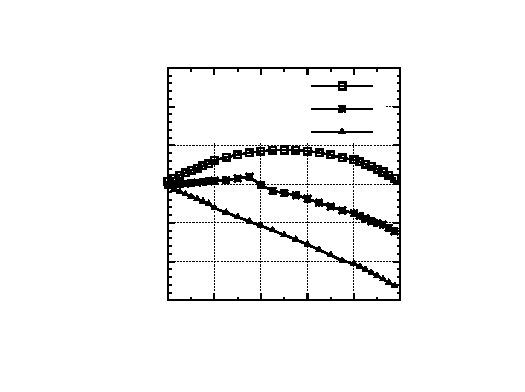
\includegraphics{figures/ethmeth-dgsol/ethmeth-dgsol}}%
    \gplfronttext
  \end{picture}%
\endgroup
\hspace*{-1.3cm}% GNUPLOT: LaTeX picture with Postscript
\begingroup
  \makeatletter
  \providecommand\color[2][]{%
    \GenericError{(gnuplot) \space\space\space\@spaces}{%
      Package color not loaded in conjunction with
      terminal option `colourtext'%
    }{See the gnuplot documentation for explanation.%
    }{Either use 'blacktext' in gnuplot or load the package
      color.sty in LaTeX.}%
    \renewcommand\color[2][]{}%
  }%
  \providecommand\includegraphics[2][]{%
    \GenericError{(gnuplot) \space\space\space\@spaces}{%
      Package graphicx or graphics not loaded%
    }{See the gnuplot documentation for explanation.%
    }{The gnuplot epslatex terminal needs graphicx.sty or graphics.sty.}%
    \renewcommand\includegraphics[2][]{}%
  }%
  \providecommand\rotatebox[2]{#2}%
  \@ifundefined{ifGPcolor}{%
    \newif\ifGPcolor
    \GPcolortrue
  }{}%
  \@ifundefined{ifGPblacktext}{%
    \newif\ifGPblacktext
    \GPblacktextfalse
  }{}%
  % define a \g@addto@macro without @ in the name:
  \let\gplgaddtomacro\g@addto@macro
  % define empty templates for all commands taking text:
  \gdef\gplbacktext{}%
  \gdef\gplfronttext{}%
  \makeatother
  \ifGPblacktext
    % no textcolor at all
    \def\colorrgb#1{}%
    \def\colorgray#1{}%
  \else
    % gray or color?
    \ifGPcolor
      \def\colorrgb#1{\color[rgb]{#1}}%
      \def\colorgray#1{\color[gray]{#1}}%
      \expandafter\def\csname LTw\endcsname{\color{white}}%
      \expandafter\def\csname LTb\endcsname{\color{black}}%
      \expandafter\def\csname LTa\endcsname{\color{black}}%
      \expandafter\def\csname LT0\endcsname{\color[rgb]{1,0,0}}%
      \expandafter\def\csname LT1\endcsname{\color[rgb]{0,1,0}}%
      \expandafter\def\csname LT2\endcsname{\color[rgb]{0,0,1}}%
      \expandafter\def\csname LT3\endcsname{\color[rgb]{1,0,1}}%
      \expandafter\def\csname LT4\endcsname{\color[rgb]{0,1,1}}%
      \expandafter\def\csname LT5\endcsname{\color[rgb]{1,1,0}}%
      \expandafter\def\csname LT6\endcsname{\color[rgb]{0,0,0}}%
      \expandafter\def\csname LT7\endcsname{\color[rgb]{1,0.3,0}}%
      \expandafter\def\csname LT8\endcsname{\color[rgb]{0.5,0.5,0.5}}%
    \else
      % gray
      \def\colorrgb#1{\color{black}}%
      \def\colorgray#1{\color[gray]{#1}}%
      \expandafter\def\csname LTw\endcsname{\color{white}}%
      \expandafter\def\csname LTb\endcsname{\color{black}}%
      \expandafter\def\csname LTa\endcsname{\color{black}}%
      \expandafter\def\csname LT0\endcsname{\color{black}}%
      \expandafter\def\csname LT1\endcsname{\color{black}}%
      \expandafter\def\csname LT2\endcsname{\color{black}}%
      \expandafter\def\csname LT3\endcsname{\color{black}}%
      \expandafter\def\csname LT4\endcsname{\color{black}}%
      \expandafter\def\csname LT5\endcsname{\color{black}}%
      \expandafter\def\csname LT6\endcsname{\color{black}}%
      \expandafter\def\csname LT7\endcsname{\color{black}}%
      \expandafter\def\csname LT8\endcsname{\color{black}}%
    \fi
  \fi
  \setlength{\unitlength}{0.0500bp}%
  \begin{picture}(5040.00,3772.00)%
    \gplgaddtomacro\gplbacktext{%
      \csname LTb\endcsname%
      \put(1547,880){\makebox(0,0)[r]{\strut{} 0}}%
      \csname LTb\endcsname%
      \put(1547,1438){\makebox(0,0)[r]{\strut{} 5}}%
      \csname LTb\endcsname%
      \put(1547,1996){\makebox(0,0)[r]{\strut{} 10}}%
      \csname LTb\endcsname%
      \put(1547,2553){\makebox(0,0)[r]{\strut{} 15}}%
      \csname LTb\endcsname%
      \put(1547,3111){\makebox(0,0)[r]{\strut{} 20}}%
      \csname LTb\endcsname%
      \put(1679,660){\makebox(0,0){\strut{} 0}}%
      \csname LTb\endcsname%
      \put(2125,660){\makebox(0,0){\strut{} 0.2}}%
      \csname LTb\endcsname%
      \put(2571,660){\makebox(0,0){\strut{} 0.4}}%
      \csname LTb\endcsname%
      \put(3018,660){\makebox(0,0){\strut{} 0.6}}%
      \csname LTb\endcsname%
      \put(3464,660){\makebox(0,0){\strut{} 0.8}}%
      \csname LTb\endcsname%
      \put(3910,660){\makebox(0,0){\strut{} 1}}%
      \put(909,1995){\rotatebox{-270}{\makebox(0,0){\strut{}$\Delta G_\textrm{sol}$ (kcal/mol)}}}%
      \put(2794,330){\makebox(0,0){\strut{}$\lambda$}}%
      \put(2794,3441){\makebox(0,0){\strut{}AcNH$_2$ $\longrightarrow$ AcOH}}%
    }%
    \gplgaddtomacro\gplfronttext{%
      \csname LTb\endcsname%
      \put(2923,2938){\makebox(0,0)[r]{\strut{}GB/SA}}%
      \csname LTb\endcsname%
      \put(2923,2718){\makebox(0,0)[r]{\strut{}TIP4P}}%
      \csname LTb\endcsname%
      \put(2923,2498){\makebox(0,0)[r]{\strut{}Gas Phase}}%
    }%
    \gplbacktext
    \put(0,0){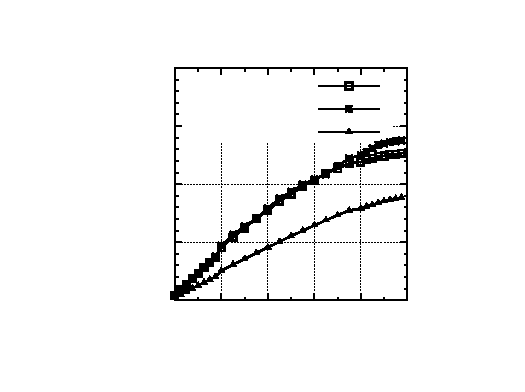
\includegraphics{figures/acamoh-dgsol/acamoh-dgsol}}%
    \gplfronttext
  \end{picture}%
\endgroup
\\
% GNUPLOT: LaTeX picture with Postscript
\begingroup
  \makeatletter
  \providecommand\color[2][]{%
    \GenericError{(gnuplot) \space\space\space\@spaces}{%
      Package color not loaded in conjunction with
      terminal option `colourtext'%
    }{See the gnuplot documentation for explanation.%
    }{Either use 'blacktext' in gnuplot or load the package
      color.sty in LaTeX.}%
    \renewcommand\color[2][]{}%
  }%
  \providecommand\includegraphics[2][]{%
    \GenericError{(gnuplot) \space\space\space\@spaces}{%
      Package graphicx or graphics not loaded%
    }{See the gnuplot documentation for explanation.%
    }{The gnuplot epslatex terminal needs graphicx.sty or graphics.sty.}%
    \renewcommand\includegraphics[2][]{}%
  }%
  \providecommand\rotatebox[2]{#2}%
  \@ifundefined{ifGPcolor}{%
    \newif\ifGPcolor
    \GPcolortrue
  }{}%
  \@ifundefined{ifGPblacktext}{%
    \newif\ifGPblacktext
    \GPblacktextfalse
  }{}%
  % define a \g@addto@macro without @ in the name:
  \let\gplgaddtomacro\g@addto@macro
  % define empty templates for all commands taking text:
  \gdef\gplbacktext{}%
  \gdef\gplfronttext{}%
  \makeatother
  \ifGPblacktext
    % no textcolor at all
    \def\colorrgb#1{}%
    \def\colorgray#1{}%
  \else
    % gray or color?
    \ifGPcolor
      \def\colorrgb#1{\color[rgb]{#1}}%
      \def\colorgray#1{\color[gray]{#1}}%
      \expandafter\def\csname LTw\endcsname{\color{white}}%
      \expandafter\def\csname LTb\endcsname{\color{black}}%
      \expandafter\def\csname LTa\endcsname{\color{black}}%
      \expandafter\def\csname LT0\endcsname{\color[rgb]{1,0,0}}%
      \expandafter\def\csname LT1\endcsname{\color[rgb]{0,1,0}}%
      \expandafter\def\csname LT2\endcsname{\color[rgb]{0,0,1}}%
      \expandafter\def\csname LT3\endcsname{\color[rgb]{1,0,1}}%
      \expandafter\def\csname LT4\endcsname{\color[rgb]{0,1,1}}%
      \expandafter\def\csname LT5\endcsname{\color[rgb]{1,1,0}}%
      \expandafter\def\csname LT6\endcsname{\color[rgb]{0,0,0}}%
      \expandafter\def\csname LT7\endcsname{\color[rgb]{1,0.3,0}}%
      \expandafter\def\csname LT8\endcsname{\color[rgb]{0.5,0.5,0.5}}%
    \else
      % gray
      \def\colorrgb#1{\color{black}}%
      \def\colorgray#1{\color[gray]{#1}}%
      \expandafter\def\csname LTw\endcsname{\color{white}}%
      \expandafter\def\csname LTb\endcsname{\color{black}}%
      \expandafter\def\csname LTa\endcsname{\color{black}}%
      \expandafter\def\csname LT0\endcsname{\color{black}}%
      \expandafter\def\csname LT1\endcsname{\color{black}}%
      \expandafter\def\csname LT2\endcsname{\color{black}}%
      \expandafter\def\csname LT3\endcsname{\color{black}}%
      \expandafter\def\csname LT4\endcsname{\color{black}}%
      \expandafter\def\csname LT5\endcsname{\color{black}}%
      \expandafter\def\csname LT6\endcsname{\color{black}}%
      \expandafter\def\csname LT7\endcsname{\color{black}}%
      \expandafter\def\csname LT8\endcsname{\color{black}}%
    \fi
  \fi
  \setlength{\unitlength}{0.0500bp}%
  \begin{picture}(5040.00,3772.00)%
    \gplgaddtomacro\gplbacktext{%
      \csname LTb\endcsname%
      \put(1547,880){\makebox(0,0)[r]{\strut{}-30}}%
      \csname LTb\endcsname%
      \put(1547,1128){\makebox(0,0)[r]{\strut{}-25}}%
      \csname LTb\endcsname%
      \put(1547,1376){\makebox(0,0)[r]{\strut{}-20}}%
      \csname LTb\endcsname%
      \put(1547,1624){\makebox(0,0)[r]{\strut{}-15}}%
      \csname LTb\endcsname%
      \put(1547,1872){\makebox(0,0)[r]{\strut{}-10}}%
      \csname LTb\endcsname%
      \put(1547,2119){\makebox(0,0)[r]{\strut{}-5}}%
      \csname LTb\endcsname%
      \put(1547,2367){\makebox(0,0)[r]{\strut{} 0}}%
      \csname LTb\endcsname%
      \put(1547,2615){\makebox(0,0)[r]{\strut{} 5}}%
      \csname LTb\endcsname%
      \put(1547,2863){\makebox(0,0)[r]{\strut{} 10}}%
      \csname LTb\endcsname%
      \put(1547,3111){\makebox(0,0)[r]{\strut{} 15}}%
      \csname LTb\endcsname%
      \put(1679,660){\makebox(0,0){\strut{} 0}}%
      \csname LTb\endcsname%
      \put(2125,660){\makebox(0,0){\strut{} 0.2}}%
      \csname LTb\endcsname%
      \put(2571,660){\makebox(0,0){\strut{} 0.4}}%
      \csname LTb\endcsname%
      \put(3018,660){\makebox(0,0){\strut{} 0.6}}%
      \csname LTb\endcsname%
      \put(3464,660){\makebox(0,0){\strut{} 0.8}}%
      \csname LTb\endcsname%
      \put(3910,660){\makebox(0,0){\strut{} 1}}%
      \put(909,1995){\rotatebox{-270}{\makebox(0,0){\strut{}$\Delta G_\textrm{sol}$ (kcal/mol)}}}%
      \put(2794,330){\makebox(0,0){\strut{}$\lambda$}}%
      \put(2794,3441){\makebox(0,0){\strut{}Cyclohexane $\longrightarrow$ THP}}%
    }%
    \gplgaddtomacro\gplfronttext{%
      \csname LTb\endcsname%
      \put(2923,2938){\makebox(0,0)[r]{\strut{}GB/SA}}%
      \csname LTb\endcsname%
      \put(2923,2718){\makebox(0,0)[r]{\strut{}TIP4P}}%
      \csname LTb\endcsname%
      \put(2923,2498){\makebox(0,0)[r]{\strut{}Gas Phase}}%
    }%
    \gplbacktext
    \put(0,0){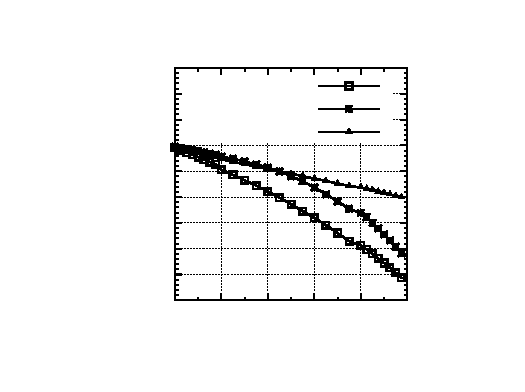
\includegraphics{figures/chexthp-dgsol/chexthp-dgsol}}%
    \gplfronttext
  \end{picture}%
\endgroup
\hspace*{-1.3cm}% GNUPLOT: LaTeX picture with Postscript
\begingroup
  \makeatletter
  \providecommand\color[2][]{%
    \GenericError{(gnuplot) \space\space\space\@spaces}{%
      Package color not loaded in conjunction with
      terminal option `colourtext'%
    }{See the gnuplot documentation for explanation.%
    }{Either use 'blacktext' in gnuplot or load the package
      color.sty in LaTeX.}%
    \renewcommand\color[2][]{}%
  }%
  \providecommand\includegraphics[2][]{%
    \GenericError{(gnuplot) \space\space\space\@spaces}{%
      Package graphicx or graphics not loaded%
    }{See the gnuplot documentation for explanation.%
    }{The gnuplot epslatex terminal needs graphicx.sty or graphics.sty.}%
    \renewcommand\includegraphics[2][]{}%
  }%
  \providecommand\rotatebox[2]{#2}%
  \@ifundefined{ifGPcolor}{%
    \newif\ifGPcolor
    \GPcolortrue
  }{}%
  \@ifundefined{ifGPblacktext}{%
    \newif\ifGPblacktext
    \GPblacktextfalse
  }{}%
  % define a \g@addto@macro without @ in the name:
  \let\gplgaddtomacro\g@addto@macro
  % define empty templates for all commands taking text:
  \gdef\gplbacktext{}%
  \gdef\gplfronttext{}%
  \makeatother
  \ifGPblacktext
    % no textcolor at all
    \def\colorrgb#1{}%
    \def\colorgray#1{}%
  \else
    % gray or color?
    \ifGPcolor
      \def\colorrgb#1{\color[rgb]{#1}}%
      \def\colorgray#1{\color[gray]{#1}}%
      \expandafter\def\csname LTw\endcsname{\color{white}}%
      \expandafter\def\csname LTb\endcsname{\color{black}}%
      \expandafter\def\csname LTa\endcsname{\color{black}}%
      \expandafter\def\csname LT0\endcsname{\color[rgb]{1,0,0}}%
      \expandafter\def\csname LT1\endcsname{\color[rgb]{0,1,0}}%
      \expandafter\def\csname LT2\endcsname{\color[rgb]{0,0,1}}%
      \expandafter\def\csname LT3\endcsname{\color[rgb]{1,0,1}}%
      \expandafter\def\csname LT4\endcsname{\color[rgb]{0,1,1}}%
      \expandafter\def\csname LT5\endcsname{\color[rgb]{1,1,0}}%
      \expandafter\def\csname LT6\endcsname{\color[rgb]{0,0,0}}%
      \expandafter\def\csname LT7\endcsname{\color[rgb]{1,0.3,0}}%
      \expandafter\def\csname LT8\endcsname{\color[rgb]{0.5,0.5,0.5}}%
    \else
      % gray
      \def\colorrgb#1{\color{black}}%
      \def\colorgray#1{\color[gray]{#1}}%
      \expandafter\def\csname LTw\endcsname{\color{white}}%
      \expandafter\def\csname LTb\endcsname{\color{black}}%
      \expandafter\def\csname LTa\endcsname{\color{black}}%
      \expandafter\def\csname LT0\endcsname{\color{black}}%
      \expandafter\def\csname LT1\endcsname{\color{black}}%
      \expandafter\def\csname LT2\endcsname{\color{black}}%
      \expandafter\def\csname LT3\endcsname{\color{black}}%
      \expandafter\def\csname LT4\endcsname{\color{black}}%
      \expandafter\def\csname LT5\endcsname{\color{black}}%
      \expandafter\def\csname LT6\endcsname{\color{black}}%
      \expandafter\def\csname LT7\endcsname{\color{black}}%
      \expandafter\def\csname LT8\endcsname{\color{black}}%
    \fi
  \fi
  \setlength{\unitlength}{0.0500bp}%
  \begin{picture}(5040.00,3772.00)%
    \gplgaddtomacro\gplbacktext{%
      \csname LTb\endcsname%
      \put(1481,880){\makebox(0,0)[r]{\strut{}-6}}%
      \csname LTb\endcsname%
      \put(1481,1252){\makebox(0,0)[r]{\strut{}-4}}%
      \csname LTb\endcsname%
      \put(1481,1624){\makebox(0,0)[r]{\strut{}-2}}%
      \csname LTb\endcsname%
      \put(1481,1996){\makebox(0,0)[r]{\strut{} 0}}%
      \csname LTb\endcsname%
      \put(1481,2367){\makebox(0,0)[r]{\strut{} 2}}%
      \csname LTb\endcsname%
      \put(1481,2739){\makebox(0,0)[r]{\strut{} 4}}%
      \csname LTb\endcsname%
      \put(1481,3111){\makebox(0,0)[r]{\strut{} 6}}%
      \csname LTb\endcsname%
      \put(1613,660){\makebox(0,0){\strut{} 0}}%
      \csname LTb\endcsname%
      \put(2059,660){\makebox(0,0){\strut{} 0.2}}%
      \csname LTb\endcsname%
      \put(2505,660){\makebox(0,0){\strut{} 0.4}}%
      \csname LTb\endcsname%
      \put(2952,660){\makebox(0,0){\strut{} 0.6}}%
      \csname LTb\endcsname%
      \put(3398,660){\makebox(0,0){\strut{} 0.8}}%
      \csname LTb\endcsname%
      \put(3844,660){\makebox(0,0){\strut{} 1}}%
      \put(975,1995){\rotatebox{-270}{\makebox(0,0){\strut{}$\Delta G_\textrm{sol}$ (kcal/mol)}}}%
      \put(2728,330){\makebox(0,0){\strut{}$\lambda$}}%
      \put(2728,3441){\makebox(0,0){\strut{}Cyclohexane $\longrightarrow$ Piperidine}}%
    }%
    \gplgaddtomacro\gplfronttext{%
      \csname LTb\endcsname%
      \put(2857,2938){\makebox(0,0)[r]{\strut{}GB/SA}}%
      \csname LTb\endcsname%
      \put(2857,2718){\makebox(0,0)[r]{\strut{}TIP4P}}%
      \csname LTb\endcsname%
      \put(2857,2498){\makebox(0,0)[r]{\strut{}Gas Phase}}%
    }%
    \gplbacktext
    \put(0,0){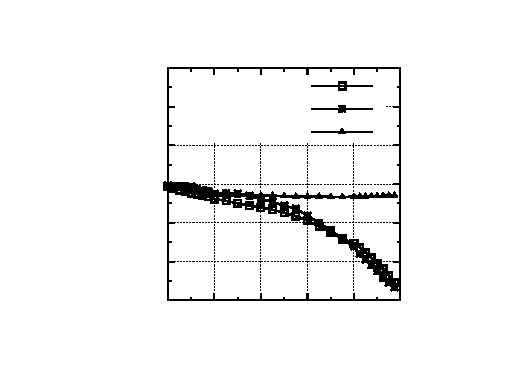
\includegraphics{figures/chexpip-dgsol/chexpip-dgsol}}%
    \gplfronttext
  \end{picture}%
\endgroup
\\
% GNUPLOT: LaTeX picture with Postscript
\begingroup
  \makeatletter
  \providecommand\color[2][]{%
    \GenericError{(gnuplot) \space\space\space\@spaces}{%
      Package color not loaded in conjunction with
      terminal option `colourtext'%
    }{See the gnuplot documentation for explanation.%
    }{Either use 'blacktext' in gnuplot or load the package
      color.sty in LaTeX.}%
    \renewcommand\color[2][]{}%
  }%
  \providecommand\includegraphics[2][]{%
    \GenericError{(gnuplot) \space\space\space\@spaces}{%
      Package graphicx or graphics not loaded%
    }{See the gnuplot documentation for explanation.%
    }{The gnuplot epslatex terminal needs graphicx.sty or graphics.sty.}%
    \renewcommand\includegraphics[2][]{}%
  }%
  \providecommand\rotatebox[2]{#2}%
  \@ifundefined{ifGPcolor}{%
    \newif\ifGPcolor
    \GPcolortrue
  }{}%
  \@ifundefined{ifGPblacktext}{%
    \newif\ifGPblacktext
    \GPblacktextfalse
  }{}%
  % define a \g@addto@macro without @ in the name:
  \let\gplgaddtomacro\g@addto@macro
  % define empty templates for all commands taking text:
  \gdef\gplbacktext{}%
  \gdef\gplfronttext{}%
  \makeatother
  \ifGPblacktext
    % no textcolor at all
    \def\colorrgb#1{}%
    \def\colorgray#1{}%
  \else
    % gray or color?
    \ifGPcolor
      \def\colorrgb#1{\color[rgb]{#1}}%
      \def\colorgray#1{\color[gray]{#1}}%
      \expandafter\def\csname LTw\endcsname{\color{white}}%
      \expandafter\def\csname LTb\endcsname{\color{black}}%
      \expandafter\def\csname LTa\endcsname{\color{black}}%
      \expandafter\def\csname LT0\endcsname{\color[rgb]{1,0,0}}%
      \expandafter\def\csname LT1\endcsname{\color[rgb]{0,1,0}}%
      \expandafter\def\csname LT2\endcsname{\color[rgb]{0,0,1}}%
      \expandafter\def\csname LT3\endcsname{\color[rgb]{1,0,1}}%
      \expandafter\def\csname LT4\endcsname{\color[rgb]{0,1,1}}%
      \expandafter\def\csname LT5\endcsname{\color[rgb]{1,1,0}}%
      \expandafter\def\csname LT6\endcsname{\color[rgb]{0,0,0}}%
      \expandafter\def\csname LT7\endcsname{\color[rgb]{1,0.3,0}}%
      \expandafter\def\csname LT8\endcsname{\color[rgb]{0.5,0.5,0.5}}%
    \else
      % gray
      \def\colorrgb#1{\color{black}}%
      \def\colorgray#1{\color[gray]{#1}}%
      \expandafter\def\csname LTw\endcsname{\color{white}}%
      \expandafter\def\csname LTb\endcsname{\color{black}}%
      \expandafter\def\csname LTa\endcsname{\color{black}}%
      \expandafter\def\csname LT0\endcsname{\color{black}}%
      \expandafter\def\csname LT1\endcsname{\color{black}}%
      \expandafter\def\csname LT2\endcsname{\color{black}}%
      \expandafter\def\csname LT3\endcsname{\color{black}}%
      \expandafter\def\csname LT4\endcsname{\color{black}}%
      \expandafter\def\csname LT5\endcsname{\color{black}}%
      \expandafter\def\csname LT6\endcsname{\color{black}}%
      \expandafter\def\csname LT7\endcsname{\color{black}}%
      \expandafter\def\csname LT8\endcsname{\color{black}}%
    \fi
  \fi
  \setlength{\unitlength}{0.0500bp}%
  \begin{picture}(5040.00,3772.00)%
    \gplgaddtomacro\gplbacktext{%
      \csname LTb\endcsname%
      \put(1481,880){\makebox(0,0)[r]{\strut{}-4}}%
      \csname LTb\endcsname%
      \put(1481,1199){\makebox(0,0)[r]{\strut{}-3}}%
      \csname LTb\endcsname%
      \put(1481,1517){\makebox(0,0)[r]{\strut{}-2}}%
      \csname LTb\endcsname%
      \put(1481,1836){\makebox(0,0)[r]{\strut{}-1}}%
      \csname LTb\endcsname%
      \put(1481,2155){\makebox(0,0)[r]{\strut{} 0}}%
      \csname LTb\endcsname%
      \put(1481,2474){\makebox(0,0)[r]{\strut{} 1}}%
      \csname LTb\endcsname%
      \put(1481,2792){\makebox(0,0)[r]{\strut{} 2}}%
      \csname LTb\endcsname%
      \put(1481,3111){\makebox(0,0)[r]{\strut{} 3}}%
      \csname LTb\endcsname%
      \put(1613,660){\makebox(0,0){\strut{} 0}}%
      \csname LTb\endcsname%
      \put(2059,660){\makebox(0,0){\strut{} 0.2}}%
      \csname LTb\endcsname%
      \put(2505,660){\makebox(0,0){\strut{} 0.4}}%
      \csname LTb\endcsname%
      \put(2952,660){\makebox(0,0){\strut{} 0.6}}%
      \csname LTb\endcsname%
      \put(3398,660){\makebox(0,0){\strut{} 0.8}}%
      \csname LTb\endcsname%
      \put(3844,660){\makebox(0,0){\strut{} 1}}%
      \put(975,1995){\rotatebox{-270}{\makebox(0,0){\strut{}$\Delta G_\textrm{sol}$ (kcal/mol)}}}%
      \put(2728,330){\makebox(0,0){\strut{}$\lambda$}}%
      \put(2728,3441){\makebox(0,0){\strut{}Propane $\longrightarrow$ $n$-PrBr}}%
    }%
    \gplgaddtomacro\gplfronttext{%
      \csname LTb\endcsname%
      \put(2857,2938){\makebox(0,0)[r]{\strut{}GB/SA}}%
      \csname LTb\endcsname%
      \put(2857,2718){\makebox(0,0)[r]{\strut{}TIP4P}}%
      \csname LTb\endcsname%
      \put(2857,2498){\makebox(0,0)[r]{\strut{}Gas Phase}}%
    }%
    \gplbacktext
    \put(0,0){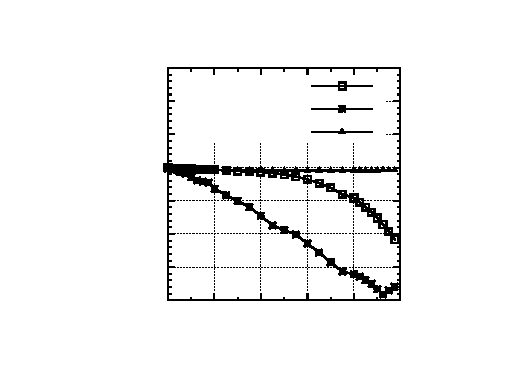
\includegraphics{figures/propbr-dgsol/propbr-dgsol}}%
    \gplfronttext
  \end{picture}%
\endgroup
\hspace*{-1.3cm}% GNUPLOT: LaTeX picture with Postscript
\begingroup
  \makeatletter
  \providecommand\color[2][]{%
    \GenericError{(gnuplot) \space\space\space\@spaces}{%
      Package color not loaded in conjunction with
      terminal option `colourtext'%
    }{See the gnuplot documentation for explanation.%
    }{Either use 'blacktext' in gnuplot or load the package
      color.sty in LaTeX.}%
    \renewcommand\color[2][]{}%
  }%
  \providecommand\includegraphics[2][]{%
    \GenericError{(gnuplot) \space\space\space\@spaces}{%
      Package graphicx or graphics not loaded%
    }{See the gnuplot documentation for explanation.%
    }{The gnuplot epslatex terminal needs graphicx.sty or graphics.sty.}%
    \renewcommand\includegraphics[2][]{}%
  }%
  \providecommand\rotatebox[2]{#2}%
  \@ifundefined{ifGPcolor}{%
    \newif\ifGPcolor
    \GPcolortrue
  }{}%
  \@ifundefined{ifGPblacktext}{%
    \newif\ifGPblacktext
    \GPblacktextfalse
  }{}%
  % define a \g@addto@macro without @ in the name:
  \let\gplgaddtomacro\g@addto@macro
  % define empty templates for all commands taking text:
  \gdef\gplbacktext{}%
  \gdef\gplfronttext{}%
  \makeatother
  \ifGPblacktext
    % no textcolor at all
    \def\colorrgb#1{}%
    \def\colorgray#1{}%
  \else
    % gray or color?
    \ifGPcolor
      \def\colorrgb#1{\color[rgb]{#1}}%
      \def\colorgray#1{\color[gray]{#1}}%
      \expandafter\def\csname LTw\endcsname{\color{white}}%
      \expandafter\def\csname LTb\endcsname{\color{black}}%
      \expandafter\def\csname LTa\endcsname{\color{black}}%
      \expandafter\def\csname LT0\endcsname{\color[rgb]{1,0,0}}%
      \expandafter\def\csname LT1\endcsname{\color[rgb]{0,1,0}}%
      \expandafter\def\csname LT2\endcsname{\color[rgb]{0,0,1}}%
      \expandafter\def\csname LT3\endcsname{\color[rgb]{1,0,1}}%
      \expandafter\def\csname LT4\endcsname{\color[rgb]{0,1,1}}%
      \expandafter\def\csname LT5\endcsname{\color[rgb]{1,1,0}}%
      \expandafter\def\csname LT6\endcsname{\color[rgb]{0,0,0}}%
      \expandafter\def\csname LT7\endcsname{\color[rgb]{1,0.3,0}}%
      \expandafter\def\csname LT8\endcsname{\color[rgb]{0.5,0.5,0.5}}%
    \else
      % gray
      \def\colorrgb#1{\color{black}}%
      \def\colorgray#1{\color[gray]{#1}}%
      \expandafter\def\csname LTw\endcsname{\color{white}}%
      \expandafter\def\csname LTb\endcsname{\color{black}}%
      \expandafter\def\csname LTa\endcsname{\color{black}}%
      \expandafter\def\csname LT0\endcsname{\color{black}}%
      \expandafter\def\csname LT1\endcsname{\color{black}}%
      \expandafter\def\csname LT2\endcsname{\color{black}}%
      \expandafter\def\csname LT3\endcsname{\color{black}}%
      \expandafter\def\csname LT4\endcsname{\color{black}}%
      \expandafter\def\csname LT5\endcsname{\color{black}}%
      \expandafter\def\csname LT6\endcsname{\color{black}}%
      \expandafter\def\csname LT7\endcsname{\color{black}}%
      \expandafter\def\csname LT8\endcsname{\color{black}}%
    \fi
  \fi
  \setlength{\unitlength}{0.0500bp}%
  \begin{picture}(5040.00,3772.00)%
    \gplgaddtomacro\gplbacktext{%
      \csname LTb\endcsname%
      \put(1481,880){\makebox(0,0)[r]{\strut{} 0}}%
      \csname LTb\endcsname%
      \put(1481,1326){\makebox(0,0)[r]{\strut{} 1}}%
      \csname LTb\endcsname%
      \put(1481,1772){\makebox(0,0)[r]{\strut{} 2}}%
      \csname LTb\endcsname%
      \put(1481,2219){\makebox(0,0)[r]{\strut{} 3}}%
      \csname LTb\endcsname%
      \put(1481,2665){\makebox(0,0)[r]{\strut{} 4}}%
      \csname LTb\endcsname%
      \put(1481,3111){\makebox(0,0)[r]{\strut{} 5}}%
      \csname LTb\endcsname%
      \put(1613,660){\makebox(0,0){\strut{} 0}}%
      \csname LTb\endcsname%
      \put(2059,660){\makebox(0,0){\strut{} 0.2}}%
      \csname LTb\endcsname%
      \put(2505,660){\makebox(0,0){\strut{} 0.4}}%
      \csname LTb\endcsname%
      \put(2952,660){\makebox(0,0){\strut{} 0.6}}%
      \csname LTb\endcsname%
      \put(3398,660){\makebox(0,0){\strut{} 0.8}}%
      \csname LTb\endcsname%
      \put(3844,660){\makebox(0,0){\strut{} 1}}%
      \put(975,1995){\rotatebox{-270}{\makebox(0,0){\strut{}$\Delta G_\textrm{sol}$ (kcal/mol)}}}%
      \put(2728,330){\makebox(0,0){\strut{}$\lambda$}}%
      \put(2728,3441){\makebox(0,0){\strut{}Propane $\longrightarrow$ iPrCl}}%
    }%
    \gplgaddtomacro\gplfronttext{%
      \csname LTb\endcsname%
      \put(2857,2938){\makebox(0,0)[r]{\strut{}GB/SA}}%
      \csname LTb\endcsname%
      \put(2857,2718){\makebox(0,0)[r]{\strut{}TIP4P}}%
      \csname LTb\endcsname%
      \put(2857,2498){\makebox(0,0)[r]{\strut{}Gas Phase}}%
    }%
    \gplbacktext
    \put(0,0){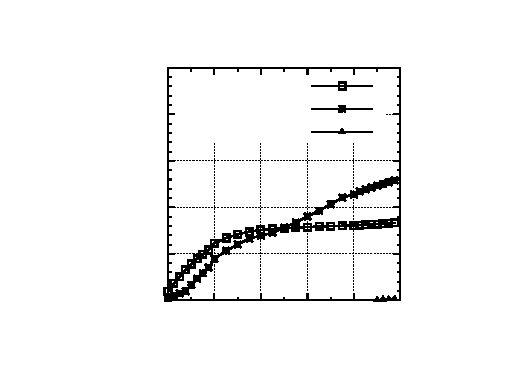
\includegraphics{figures/clprop-dgsol/clprop-dgsol}}%
    \gplfronttext
  \end{picture}%
\endgroup
\\
\caption{Selected trajectories for $\Delta G_\textrm{sol}$ from the small perturbations (Table \ref{small}) series.}
\label{dgsolsm1}
\end{figure}

\begin{figure}[p]
\centering
% GNUPLOT: LaTeX picture with Postscript
\begingroup
  \makeatletter
  \providecommand\color[2][]{%
    \GenericError{(gnuplot) \space\space\space\@spaces}{%
      Package color not loaded in conjunction with
      terminal option `colourtext'%
    }{See the gnuplot documentation for explanation.%
    }{Either use 'blacktext' in gnuplot or load the package
      color.sty in LaTeX.}%
    \renewcommand\color[2][]{}%
  }%
  \providecommand\includegraphics[2][]{%
    \GenericError{(gnuplot) \space\space\space\@spaces}{%
      Package graphicx or graphics not loaded%
    }{See the gnuplot documentation for explanation.%
    }{The gnuplot epslatex terminal needs graphicx.sty or graphics.sty.}%
    \renewcommand\includegraphics[2][]{}%
  }%
  \providecommand\rotatebox[2]{#2}%
  \@ifundefined{ifGPcolor}{%
    \newif\ifGPcolor
    \GPcolortrue
  }{}%
  \@ifundefined{ifGPblacktext}{%
    \newif\ifGPblacktext
    \GPblacktextfalse
  }{}%
  % define a \g@addto@macro without @ in the name:
  \let\gplgaddtomacro\g@addto@macro
  % define empty templates for all commands taking text:
  \gdef\gplbacktext{}%
  \gdef\gplfronttext{}%
  \makeatother
  \ifGPblacktext
    % no textcolor at all
    \def\colorrgb#1{}%
    \def\colorgray#1{}%
  \else
    % gray or color?
    \ifGPcolor
      \def\colorrgb#1{\color[rgb]{#1}}%
      \def\colorgray#1{\color[gray]{#1}}%
      \expandafter\def\csname LTw\endcsname{\color{white}}%
      \expandafter\def\csname LTb\endcsname{\color{black}}%
      \expandafter\def\csname LTa\endcsname{\color{black}}%
      \expandafter\def\csname LT0\endcsname{\color[rgb]{1,0,0}}%
      \expandafter\def\csname LT1\endcsname{\color[rgb]{0,1,0}}%
      \expandafter\def\csname LT2\endcsname{\color[rgb]{0,0,1}}%
      \expandafter\def\csname LT3\endcsname{\color[rgb]{1,0,1}}%
      \expandafter\def\csname LT4\endcsname{\color[rgb]{0,1,1}}%
      \expandafter\def\csname LT5\endcsname{\color[rgb]{1,1,0}}%
      \expandafter\def\csname LT6\endcsname{\color[rgb]{0,0,0}}%
      \expandafter\def\csname LT7\endcsname{\color[rgb]{1,0.3,0}}%
      \expandafter\def\csname LT8\endcsname{\color[rgb]{0.5,0.5,0.5}}%
    \else
      % gray
      \def\colorrgb#1{\color{black}}%
      \def\colorgray#1{\color[gray]{#1}}%
      \expandafter\def\csname LTw\endcsname{\color{white}}%
      \expandafter\def\csname LTb\endcsname{\color{black}}%
      \expandafter\def\csname LTa\endcsname{\color{black}}%
      \expandafter\def\csname LT0\endcsname{\color{black}}%
      \expandafter\def\csname LT1\endcsname{\color{black}}%
      \expandafter\def\csname LT2\endcsname{\color{black}}%
      \expandafter\def\csname LT3\endcsname{\color{black}}%
      \expandafter\def\csname LT4\endcsname{\color{black}}%
      \expandafter\def\csname LT5\endcsname{\color{black}}%
      \expandafter\def\csname LT6\endcsname{\color{black}}%
      \expandafter\def\csname LT7\endcsname{\color{black}}%
      \expandafter\def\csname LT8\endcsname{\color{black}}%
    \fi
  \fi
  \setlength{\unitlength}{0.0500bp}%
  \begin{picture}(5040.00,3772.00)%
    \gplgaddtomacro\gplbacktext{%
      \csname LTb\endcsname%
      \put(1547,880){\makebox(0,0)[r]{\strut{}-40}}%
      \csname LTb\endcsname%
      \put(1547,1252){\makebox(0,0)[r]{\strut{}-30}}%
      \csname LTb\endcsname%
      \put(1547,1624){\makebox(0,0)[r]{\strut{}-20}}%
      \csname LTb\endcsname%
      \put(1547,1996){\makebox(0,0)[r]{\strut{}-10}}%
      \csname LTb\endcsname%
      \put(1547,2367){\makebox(0,0)[r]{\strut{} 0}}%
      \csname LTb\endcsname%
      \put(1547,2739){\makebox(0,0)[r]{\strut{} 10}}%
      \csname LTb\endcsname%
      \put(1547,3111){\makebox(0,0)[r]{\strut{} 20}}%
      \csname LTb\endcsname%
      \put(1679,660){\makebox(0,0){\strut{} 0}}%
      \csname LTb\endcsname%
      \put(2125,660){\makebox(0,0){\strut{} 0.2}}%
      \csname LTb\endcsname%
      \put(2571,660){\makebox(0,0){\strut{} 0.4}}%
      \csname LTb\endcsname%
      \put(3018,660){\makebox(0,0){\strut{} 0.6}}%
      \csname LTb\endcsname%
      \put(3464,660){\makebox(0,0){\strut{} 0.8}}%
      \csname LTb\endcsname%
      \put(3910,660){\makebox(0,0){\strut{} 1}}%
      \put(909,1995){\rotatebox{-270}{\makebox(0,0){\strut{}$\Delta G_\textrm{sol}$ (kcal/mol)}}}%
      \put(2794,330){\makebox(0,0){\strut{}$\lambda$}}%
      \put(2794,3441){\makebox(0,0){\strut{}Benzene $\longrightarrow$ Pyridine}}%
    }%
    \gplgaddtomacro\gplfronttext{%
      \csname LTb\endcsname%
      \put(2923,2938){\makebox(0,0)[r]{\strut{}GB/SA}}%
      \csname LTb\endcsname%
      \put(2923,2718){\makebox(0,0)[r]{\strut{}TIP4P}}%
      \csname LTb\endcsname%
      \put(2923,2498){\makebox(0,0)[r]{\strut{}Gas Phase}}%
    }%
    \gplbacktext
    \put(0,0){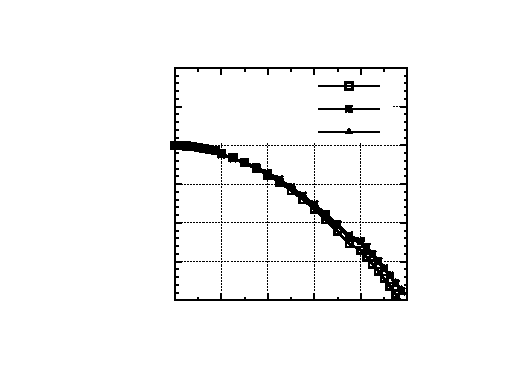
\includegraphics{figures/benzpyr-dgsol/benzpyr-dgsol}}%
    \gplfronttext
  \end{picture}%
\endgroup
\hspace*{-1.3cm}% GNUPLOT: LaTeX picture with Postscript
\begingroup
  \makeatletter
  \providecommand\color[2][]{%
    \GenericError{(gnuplot) \space\space\space\@spaces}{%
      Package color not loaded in conjunction with
      terminal option `colourtext'%
    }{See the gnuplot documentation for explanation.%
    }{Either use 'blacktext' in gnuplot or load the package
      color.sty in LaTeX.}%
    \renewcommand\color[2][]{}%
  }%
  \providecommand\includegraphics[2][]{%
    \GenericError{(gnuplot) \space\space\space\@spaces}{%
      Package graphicx or graphics not loaded%
    }{See the gnuplot documentation for explanation.%
    }{The gnuplot epslatex terminal needs graphicx.sty or graphics.sty.}%
    \renewcommand\includegraphics[2][]{}%
  }%
  \providecommand\rotatebox[2]{#2}%
  \@ifundefined{ifGPcolor}{%
    \newif\ifGPcolor
    \GPcolortrue
  }{}%
  \@ifundefined{ifGPblacktext}{%
    \newif\ifGPblacktext
    \GPblacktextfalse
  }{}%
  % define a \g@addto@macro without @ in the name:
  \let\gplgaddtomacro\g@addto@macro
  % define empty templates for all commands taking text:
  \gdef\gplbacktext{}%
  \gdef\gplfronttext{}%
  \makeatother
  \ifGPblacktext
    % no textcolor at all
    \def\colorrgb#1{}%
    \def\colorgray#1{}%
  \else
    % gray or color?
    \ifGPcolor
      \def\colorrgb#1{\color[rgb]{#1}}%
      \def\colorgray#1{\color[gray]{#1}}%
      \expandafter\def\csname LTw\endcsname{\color{white}}%
      \expandafter\def\csname LTb\endcsname{\color{black}}%
      \expandafter\def\csname LTa\endcsname{\color{black}}%
      \expandafter\def\csname LT0\endcsname{\color[rgb]{1,0,0}}%
      \expandafter\def\csname LT1\endcsname{\color[rgb]{0,1,0}}%
      \expandafter\def\csname LT2\endcsname{\color[rgb]{0,0,1}}%
      \expandafter\def\csname LT3\endcsname{\color[rgb]{1,0,1}}%
      \expandafter\def\csname LT4\endcsname{\color[rgb]{0,1,1}}%
      \expandafter\def\csname LT5\endcsname{\color[rgb]{1,1,0}}%
      \expandafter\def\csname LT6\endcsname{\color[rgb]{0,0,0}}%
      \expandafter\def\csname LT7\endcsname{\color[rgb]{1,0.3,0}}%
      \expandafter\def\csname LT8\endcsname{\color[rgb]{0.5,0.5,0.5}}%
    \else
      % gray
      \def\colorrgb#1{\color{black}}%
      \def\colorgray#1{\color[gray]{#1}}%
      \expandafter\def\csname LTw\endcsname{\color{white}}%
      \expandafter\def\csname LTb\endcsname{\color{black}}%
      \expandafter\def\csname LTa\endcsname{\color{black}}%
      \expandafter\def\csname LT0\endcsname{\color{black}}%
      \expandafter\def\csname LT1\endcsname{\color{black}}%
      \expandafter\def\csname LT2\endcsname{\color{black}}%
      \expandafter\def\csname LT3\endcsname{\color{black}}%
      \expandafter\def\csname LT4\endcsname{\color{black}}%
      \expandafter\def\csname LT5\endcsname{\color{black}}%
      \expandafter\def\csname LT6\endcsname{\color{black}}%
      \expandafter\def\csname LT7\endcsname{\color{black}}%
      \expandafter\def\csname LT8\endcsname{\color{black}}%
    \fi
  \fi
  \setlength{\unitlength}{0.0500bp}%
  \begin{picture}(5040.00,3772.00)%
    \gplgaddtomacro\gplbacktext{%
      \csname LTb\endcsname%
      \put(1547,880){\makebox(0,0)[r]{\strut{}-10}}%
      \csname LTb\endcsname%
      \put(1547,1177){\makebox(0,0)[r]{\strut{}-8}}%
      \csname LTb\endcsname%
      \put(1547,1475){\makebox(0,0)[r]{\strut{}-6}}%
      \csname LTb\endcsname%
      \put(1547,1772){\makebox(0,0)[r]{\strut{}-4}}%
      \csname LTb\endcsname%
      \put(1547,2070){\makebox(0,0)[r]{\strut{}-2}}%
      \csname LTb\endcsname%
      \put(1547,2367){\makebox(0,0)[r]{\strut{} 0}}%
      \csname LTb\endcsname%
      \put(1547,2665){\makebox(0,0)[r]{\strut{} 2}}%
      \csname LTb\endcsname%
      \put(1547,2962){\makebox(0,0)[r]{\strut{} 4}}%
      \csname LTb\endcsname%
      \put(1679,660){\makebox(0,0){\strut{} 0}}%
      \csname LTb\endcsname%
      \put(2125,660){\makebox(0,0){\strut{} 0.2}}%
      \csname LTb\endcsname%
      \put(2571,660){\makebox(0,0){\strut{} 0.4}}%
      \csname LTb\endcsname%
      \put(3018,660){\makebox(0,0){\strut{} 0.6}}%
      \csname LTb\endcsname%
      \put(3464,660){\makebox(0,0){\strut{} 0.8}}%
      \csname LTb\endcsname%
      \put(3910,660){\makebox(0,0){\strut{} 1}}%
      \put(909,1995){\rotatebox{-270}{\makebox(0,0){\strut{}$\Delta G_\textrm{sol}$ (kcal/mol)}}}%
      \put(2794,330){\makebox(0,0){\strut{}$\lambda$}}%
      \put(2794,3441){\makebox(0,0){\strut{}PhCH$_3$ $\longrightarrow$ PhOH}}%
    }%
    \gplgaddtomacro\gplfronttext{%
      \csname LTb\endcsname%
      \put(2923,2938){\makebox(0,0)[r]{\strut{}GB/SA}}%
      \csname LTb\endcsname%
      \put(2923,2718){\makebox(0,0)[r]{\strut{}TIP4P}}%
      \csname LTb\endcsname%
      \put(2923,2498){\makebox(0,0)[r]{\strut{}Gas Phase}}%
    }%
    \gplbacktext
    \put(0,0){\includegraphics{figures/tolphoh-dgsol/tolphoh-dgsol}}%
    \gplfronttext
  \end{picture}%
\endgroup
\\
% GNUPLOT: LaTeX picture with Postscript
\begingroup
  \makeatletter
  \providecommand\color[2][]{%
    \GenericError{(gnuplot) \space\space\space\@spaces}{%
      Package color not loaded in conjunction with
      terminal option `colourtext'%
    }{See the gnuplot documentation for explanation.%
    }{Either use 'blacktext' in gnuplot or load the package
      color.sty in LaTeX.}%
    \renewcommand\color[2][]{}%
  }%
  \providecommand\includegraphics[2][]{%
    \GenericError{(gnuplot) \space\space\space\@spaces}{%
      Package graphicx or graphics not loaded%
    }{See the gnuplot documentation for explanation.%
    }{The gnuplot epslatex terminal needs graphicx.sty or graphics.sty.}%
    \renewcommand\includegraphics[2][]{}%
  }%
  \providecommand\rotatebox[2]{#2}%
  \@ifundefined{ifGPcolor}{%
    \newif\ifGPcolor
    \GPcolortrue
  }{}%
  \@ifundefined{ifGPblacktext}{%
    \newif\ifGPblacktext
    \GPblacktextfalse
  }{}%
  % define a \g@addto@macro without @ in the name:
  \let\gplgaddtomacro\g@addto@macro
  % define empty templates for all commands taking text:
  \gdef\gplbacktext{}%
  \gdef\gplfronttext{}%
  \makeatother
  \ifGPblacktext
    % no textcolor at all
    \def\colorrgb#1{}%
    \def\colorgray#1{}%
  \else
    % gray or color?
    \ifGPcolor
      \def\colorrgb#1{\color[rgb]{#1}}%
      \def\colorgray#1{\color[gray]{#1}}%
      \expandafter\def\csname LTw\endcsname{\color{white}}%
      \expandafter\def\csname LTb\endcsname{\color{black}}%
      \expandafter\def\csname LTa\endcsname{\color{black}}%
      \expandafter\def\csname LT0\endcsname{\color[rgb]{1,0,0}}%
      \expandafter\def\csname LT1\endcsname{\color[rgb]{0,1,0}}%
      \expandafter\def\csname LT2\endcsname{\color[rgb]{0,0,1}}%
      \expandafter\def\csname LT3\endcsname{\color[rgb]{1,0,1}}%
      \expandafter\def\csname LT4\endcsname{\color[rgb]{0,1,1}}%
      \expandafter\def\csname LT5\endcsname{\color[rgb]{1,1,0}}%
      \expandafter\def\csname LT6\endcsname{\color[rgb]{0,0,0}}%
      \expandafter\def\csname LT7\endcsname{\color[rgb]{1,0.3,0}}%
      \expandafter\def\csname LT8\endcsname{\color[rgb]{0.5,0.5,0.5}}%
    \else
      % gray
      \def\colorrgb#1{\color{black}}%
      \def\colorgray#1{\color[gray]{#1}}%
      \expandafter\def\csname LTw\endcsname{\color{white}}%
      \expandafter\def\csname LTb\endcsname{\color{black}}%
      \expandafter\def\csname LTa\endcsname{\color{black}}%
      \expandafter\def\csname LT0\endcsname{\color{black}}%
      \expandafter\def\csname LT1\endcsname{\color{black}}%
      \expandafter\def\csname LT2\endcsname{\color{black}}%
      \expandafter\def\csname LT3\endcsname{\color{black}}%
      \expandafter\def\csname LT4\endcsname{\color{black}}%
      \expandafter\def\csname LT5\endcsname{\color{black}}%
      \expandafter\def\csname LT6\endcsname{\color{black}}%
      \expandafter\def\csname LT7\endcsname{\color{black}}%
      \expandafter\def\csname LT8\endcsname{\color{black}}%
    \fi
  \fi
  \setlength{\unitlength}{0.0500bp}%
  \begin{picture}(5040.00,3772.00)%
    \gplgaddtomacro\gplbacktext{%
      \csname LTb\endcsname%
      \put(1547,880){\makebox(0,0)[r]{\strut{}-10}}%
      \csname LTb\endcsname%
      \put(1547,1177){\makebox(0,0)[r]{\strut{}-8}}%
      \csname LTb\endcsname%
      \put(1547,1475){\makebox(0,0)[r]{\strut{}-6}}%
      \csname LTb\endcsname%
      \put(1547,1772){\makebox(0,0)[r]{\strut{}-4}}%
      \csname LTb\endcsname%
      \put(1547,2070){\makebox(0,0)[r]{\strut{}-2}}%
      \csname LTb\endcsname%
      \put(1547,2367){\makebox(0,0)[r]{\strut{} 0}}%
      \csname LTb\endcsname%
      \put(1547,2665){\makebox(0,0)[r]{\strut{} 2}}%
      \csname LTb\endcsname%
      \put(1547,2962){\makebox(0,0)[r]{\strut{} 4}}%
      \csname LTb\endcsname%
      \put(1679,660){\makebox(0,0){\strut{} 0}}%
      \csname LTb\endcsname%
      \put(2125,660){\makebox(0,0){\strut{} 0.2}}%
      \csname LTb\endcsname%
      \put(2571,660){\makebox(0,0){\strut{} 0.4}}%
      \csname LTb\endcsname%
      \put(3018,660){\makebox(0,0){\strut{} 0.6}}%
      \csname LTb\endcsname%
      \put(3464,660){\makebox(0,0){\strut{} 0.8}}%
      \csname LTb\endcsname%
      \put(3910,660){\makebox(0,0){\strut{} 1}}%
      \put(909,1995){\rotatebox{-270}{\makebox(0,0){\strut{}$\Delta G_\textrm{sol}$ (kcal/mol)}}}%
      \put(2794,330){\makebox(0,0){\strut{}$\lambda$}}%
      \put(2794,3441){\makebox(0,0){\strut{}PhCH$_3$ $\longrightarrow$ PhNH$_2$}}%
    }%
    \gplgaddtomacro\gplfronttext{%
      \csname LTb\endcsname%
      \put(2923,2938){\makebox(0,0)[r]{\strut{}GB/SA}}%
      \csname LTb\endcsname%
      \put(2923,2718){\makebox(0,0)[r]{\strut{}TIP4P}}%
      \csname LTb\endcsname%
      \put(2923,2498){\makebox(0,0)[r]{\strut{}Gas Phase}}%
    }%
    \gplbacktext
    \put(0,0){\includegraphics{figures/tolanil-dgsol/tolanil-dgsol}}%
    \gplfronttext
  \end{picture}%
\endgroup
\hspace*{-1.3cm}% GNUPLOT: LaTeX picture with Postscript
\begingroup
  \makeatletter
  \providecommand\color[2][]{%
    \GenericError{(gnuplot) \space\space\space\@spaces}{%
      Package color not loaded in conjunction with
      terminal option `colourtext'%
    }{See the gnuplot documentation for explanation.%
    }{Either use 'blacktext' in gnuplot or load the package
      color.sty in LaTeX.}%
    \renewcommand\color[2][]{}%
  }%
  \providecommand\includegraphics[2][]{%
    \GenericError{(gnuplot) \space\space\space\@spaces}{%
      Package graphicx or graphics not loaded%
    }{See the gnuplot documentation for explanation.%
    }{The gnuplot epslatex terminal needs graphicx.sty or graphics.sty.}%
    \renewcommand\includegraphics[2][]{}%
  }%
  \providecommand\rotatebox[2]{#2}%
  \@ifundefined{ifGPcolor}{%
    \newif\ifGPcolor
    \GPcolortrue
  }{}%
  \@ifundefined{ifGPblacktext}{%
    \newif\ifGPblacktext
    \GPblacktextfalse
  }{}%
  % define a \g@addto@macro without @ in the name:
  \let\gplgaddtomacro\g@addto@macro
  % define empty templates for all commands taking text:
  \gdef\gplbacktext{}%
  \gdef\gplfronttext{}%
  \makeatother
  \ifGPblacktext
    % no textcolor at all
    \def\colorrgb#1{}%
    \def\colorgray#1{}%
  \else
    % gray or color?
    \ifGPcolor
      \def\colorrgb#1{\color[rgb]{#1}}%
      \def\colorgray#1{\color[gray]{#1}}%
      \expandafter\def\csname LTw\endcsname{\color{white}}%
      \expandafter\def\csname LTb\endcsname{\color{black}}%
      \expandafter\def\csname LTa\endcsname{\color{black}}%
      \expandafter\def\csname LT0\endcsname{\color[rgb]{1,0,0}}%
      \expandafter\def\csname LT1\endcsname{\color[rgb]{0,1,0}}%
      \expandafter\def\csname LT2\endcsname{\color[rgb]{0,0,1}}%
      \expandafter\def\csname LT3\endcsname{\color[rgb]{1,0,1}}%
      \expandafter\def\csname LT4\endcsname{\color[rgb]{0,1,1}}%
      \expandafter\def\csname LT5\endcsname{\color[rgb]{1,1,0}}%
      \expandafter\def\csname LT6\endcsname{\color[rgb]{0,0,0}}%
      \expandafter\def\csname LT7\endcsname{\color[rgb]{1,0.3,0}}%
      \expandafter\def\csname LT8\endcsname{\color[rgb]{0.5,0.5,0.5}}%
    \else
      % gray
      \def\colorrgb#1{\color{black}}%
      \def\colorgray#1{\color[gray]{#1}}%
      \expandafter\def\csname LTw\endcsname{\color{white}}%
      \expandafter\def\csname LTb\endcsname{\color{black}}%
      \expandafter\def\csname LTa\endcsname{\color{black}}%
      \expandafter\def\csname LT0\endcsname{\color{black}}%
      \expandafter\def\csname LT1\endcsname{\color{black}}%
      \expandafter\def\csname LT2\endcsname{\color{black}}%
      \expandafter\def\csname LT3\endcsname{\color{black}}%
      \expandafter\def\csname LT4\endcsname{\color{black}}%
      \expandafter\def\csname LT5\endcsname{\color{black}}%
      \expandafter\def\csname LT6\endcsname{\color{black}}%
      \expandafter\def\csname LT7\endcsname{\color{black}}%
      \expandafter\def\csname LT8\endcsname{\color{black}}%
    \fi
  \fi
  \setlength{\unitlength}{0.0500bp}%
  \begin{picture}(5040.00,3772.00)%
    \gplgaddtomacro\gplbacktext{%
      \csname LTb\endcsname%
      \put(1547,880){\makebox(0,0)[r]{\strut{} 0}}%
      \csname LTb\endcsname%
      \put(1547,1252){\makebox(0,0)[r]{\strut{} 2}}%
      \csname LTb\endcsname%
      \put(1547,1624){\makebox(0,0)[r]{\strut{} 4}}%
      \csname LTb\endcsname%
      \put(1547,1996){\makebox(0,0)[r]{\strut{} 6}}%
      \csname LTb\endcsname%
      \put(1547,2367){\makebox(0,0)[r]{\strut{} 8}}%
      \csname LTb\endcsname%
      \put(1547,2739){\makebox(0,0)[r]{\strut{} 10}}%
      \csname LTb\endcsname%
      \put(1547,3111){\makebox(0,0)[r]{\strut{} 12}}%
      \csname LTb\endcsname%
      \put(1679,660){\makebox(0,0){\strut{} 0}}%
      \csname LTb\endcsname%
      \put(2125,660){\makebox(0,0){\strut{} 0.2}}%
      \csname LTb\endcsname%
      \put(2571,660){\makebox(0,0){\strut{} 0.4}}%
      \csname LTb\endcsname%
      \put(3018,660){\makebox(0,0){\strut{} 0.6}}%
      \csname LTb\endcsname%
      \put(3464,660){\makebox(0,0){\strut{} 0.8}}%
      \csname LTb\endcsname%
      \put(3910,660){\makebox(0,0){\strut{} 1}}%
      \put(909,1995){\rotatebox{-270}{\makebox(0,0){\strut{}$\Delta G_\textrm{sol}$ (kcal/mol)}}}%
      \put(2794,330){\makebox(0,0){\strut{}$\lambda$}}%
      \put(2794,3441){\makebox(0,0){\strut{}Piperidine $\longrightarrow$ THP}}%
    }%
    \gplgaddtomacro\gplfronttext{%
      \csname LTb\endcsname%
      \put(2923,2938){\makebox(0,0)[r]{\strut{}GB/SA}}%
      \csname LTb\endcsname%
      \put(2923,2718){\makebox(0,0)[r]{\strut{}TIP4P}}%
      \csname LTb\endcsname%
      \put(2923,2498){\makebox(0,0)[r]{\strut{}Gas Phase}}%
    }%
    \gplbacktext
    \put(0,0){\includegraphics{figures/thioananis-dgsol/thioananis-dgsol}}%
    \gplfronttext
  \end{picture}%
\endgroup
\\
% GNUPLOT: LaTeX picture with Postscript
\begingroup
  \makeatletter
  \providecommand\color[2][]{%
    \GenericError{(gnuplot) \space\space\space\@spaces}{%
      Package color not loaded in conjunction with
      terminal option `colourtext'%
    }{See the gnuplot documentation for explanation.%
    }{Either use 'blacktext' in gnuplot or load the package
      color.sty in LaTeX.}%
    \renewcommand\color[2][]{}%
  }%
  \providecommand\includegraphics[2][]{%
    \GenericError{(gnuplot) \space\space\space\@spaces}{%
      Package graphicx or graphics not loaded%
    }{See the gnuplot documentation for explanation.%
    }{The gnuplot epslatex terminal needs graphicx.sty or graphics.sty.}%
    \renewcommand\includegraphics[2][]{}%
  }%
  \providecommand\rotatebox[2]{#2}%
  \@ifundefined{ifGPcolor}{%
    \newif\ifGPcolor
    \GPcolortrue
  }{}%
  \@ifundefined{ifGPblacktext}{%
    \newif\ifGPblacktext
    \GPblacktextfalse
  }{}%
  % define a \g@addto@macro without @ in the name:
  \let\gplgaddtomacro\g@addto@macro
  % define empty templates for all commands taking text:
  \gdef\gplbacktext{}%
  \gdef\gplfronttext{}%
  \makeatother
  \ifGPblacktext
    % no textcolor at all
    \def\colorrgb#1{}%
    \def\colorgray#1{}%
  \else
    % gray or color?
    \ifGPcolor
      \def\colorrgb#1{\color[rgb]{#1}}%
      \def\colorgray#1{\color[gray]{#1}}%
      \expandafter\def\csname LTw\endcsname{\color{white}}%
      \expandafter\def\csname LTb\endcsname{\color{black}}%
      \expandafter\def\csname LTa\endcsname{\color{black}}%
      \expandafter\def\csname LT0\endcsname{\color[rgb]{1,0,0}}%
      \expandafter\def\csname LT1\endcsname{\color[rgb]{0,1,0}}%
      \expandafter\def\csname LT2\endcsname{\color[rgb]{0,0,1}}%
      \expandafter\def\csname LT3\endcsname{\color[rgb]{1,0,1}}%
      \expandafter\def\csname LT4\endcsname{\color[rgb]{0,1,1}}%
      \expandafter\def\csname LT5\endcsname{\color[rgb]{1,1,0}}%
      \expandafter\def\csname LT6\endcsname{\color[rgb]{0,0,0}}%
      \expandafter\def\csname LT7\endcsname{\color[rgb]{1,0.3,0}}%
      \expandafter\def\csname LT8\endcsname{\color[rgb]{0.5,0.5,0.5}}%
    \else
      % gray
      \def\colorrgb#1{\color{black}}%
      \def\colorgray#1{\color[gray]{#1}}%
      \expandafter\def\csname LTw\endcsname{\color{white}}%
      \expandafter\def\csname LTb\endcsname{\color{black}}%
      \expandafter\def\csname LTa\endcsname{\color{black}}%
      \expandafter\def\csname LT0\endcsname{\color{black}}%
      \expandafter\def\csname LT1\endcsname{\color{black}}%
      \expandafter\def\csname LT2\endcsname{\color{black}}%
      \expandafter\def\csname LT3\endcsname{\color{black}}%
      \expandafter\def\csname LT4\endcsname{\color{black}}%
      \expandafter\def\csname LT5\endcsname{\color{black}}%
      \expandafter\def\csname LT6\endcsname{\color{black}}%
      \expandafter\def\csname LT7\endcsname{\color{black}}%
      \expandafter\def\csname LT8\endcsname{\color{black}}%
    \fi
  \fi
  \setlength{\unitlength}{0.0500bp}%
  \begin{picture}(5040.00,3772.00)%
    \gplgaddtomacro\gplbacktext{%
      \csname LTb\endcsname%
      \put(1547,880){\makebox(0,0)[r]{\strut{}-20}}%
      \csname LTb\endcsname%
      \put(1547,1252){\makebox(0,0)[r]{\strut{}-15}}%
      \csname LTb\endcsname%
      \put(1547,1624){\makebox(0,0)[r]{\strut{}-10}}%
      \csname LTb\endcsname%
      \put(1547,1996){\makebox(0,0)[r]{\strut{}-5}}%
      \csname LTb\endcsname%
      \put(1547,2367){\makebox(0,0)[r]{\strut{} 0}}%
      \csname LTb\endcsname%
      \put(1547,2739){\makebox(0,0)[r]{\strut{} 5}}%
      \csname LTb\endcsname%
      \put(1547,3111){\makebox(0,0)[r]{\strut{} 10}}%
      \csname LTb\endcsname%
      \put(1679,660){\makebox(0,0){\strut{} 0}}%
      \csname LTb\endcsname%
      \put(2125,660){\makebox(0,0){\strut{} 0.2}}%
      \csname LTb\endcsname%
      \put(2571,660){\makebox(0,0){\strut{} 0.4}}%
      \csname LTb\endcsname%
      \put(3018,660){\makebox(0,0){\strut{} 0.6}}%
      \csname LTb\endcsname%
      \put(3464,660){\makebox(0,0){\strut{} 0.8}}%
      \csname LTb\endcsname%
      \put(3910,660){\makebox(0,0){\strut{} 1}}%
      \put(909,1995){\rotatebox{-270}{\makebox(0,0){\strut{}$\Delta G_\textrm{sol}$ (kcal/mol)}}}%
      \put(2794,330){\makebox(0,0){\strut{}$\lambda$}}%
      \put(2794,3441){\makebox(0,0){\strut{}N(CH$_3$)$_3$ $\longrightarrow$ Acetone}}%
    }%
    \gplgaddtomacro\gplfronttext{%
      \csname LTb\endcsname%
      \put(2923,2938){\makebox(0,0)[r]{\strut{}GB/SA}}%
      \csname LTb\endcsname%
      \put(2923,2718){\makebox(0,0)[r]{\strut{}TIP4P}}%
      \csname LTb\endcsname%
      \put(2923,2498){\makebox(0,0)[r]{\strut{}Gas Phase}}%
    }%
    \gplbacktext
    \put(0,0){\includegraphics{figures/trimeac-dgsol/trimeac-dgsol}}%
    \gplfronttext
  \end{picture}%
\endgroup
\hspace*{-1.3cm}% GNUPLOT: LaTeX picture with Postscript
\begingroup
  \makeatletter
  \providecommand\color[2][]{%
    \GenericError{(gnuplot) \space\space\space\@spaces}{%
      Package color not loaded in conjunction with
      terminal option `colourtext'%
    }{See the gnuplot documentation for explanation.%
    }{Either use 'blacktext' in gnuplot or load the package
      color.sty in LaTeX.}%
    \renewcommand\color[2][]{}%
  }%
  \providecommand\includegraphics[2][]{%
    \GenericError{(gnuplot) \space\space\space\@spaces}{%
      Package graphicx or graphics not loaded%
    }{See the gnuplot documentation for explanation.%
    }{The gnuplot epslatex terminal needs graphicx.sty or graphics.sty.}%
    \renewcommand\includegraphics[2][]{}%
  }%
  \providecommand\rotatebox[2]{#2}%
  \@ifundefined{ifGPcolor}{%
    \newif\ifGPcolor
    \GPcolortrue
  }{}%
  \@ifundefined{ifGPblacktext}{%
    \newif\ifGPblacktext
    \GPblacktextfalse
  }{}%
  % define a \g@addto@macro without @ in the name:
  \let\gplgaddtomacro\g@addto@macro
  % define empty templates for all commands taking text:
  \gdef\gplbacktext{}%
  \gdef\gplfronttext{}%
  \makeatother
  \ifGPblacktext
    % no textcolor at all
    \def\colorrgb#1{}%
    \def\colorgray#1{}%
  \else
    % gray or color?
    \ifGPcolor
      \def\colorrgb#1{\color[rgb]{#1}}%
      \def\colorgray#1{\color[gray]{#1}}%
      \expandafter\def\csname LTw\endcsname{\color{white}}%
      \expandafter\def\csname LTb\endcsname{\color{black}}%
      \expandafter\def\csname LTa\endcsname{\color{black}}%
      \expandafter\def\csname LT0\endcsname{\color[rgb]{1,0,0}}%
      \expandafter\def\csname LT1\endcsname{\color[rgb]{0,1,0}}%
      \expandafter\def\csname LT2\endcsname{\color[rgb]{0,0,1}}%
      \expandafter\def\csname LT3\endcsname{\color[rgb]{1,0,1}}%
      \expandafter\def\csname LT4\endcsname{\color[rgb]{0,1,1}}%
      \expandafter\def\csname LT5\endcsname{\color[rgb]{1,1,0}}%
      \expandafter\def\csname LT6\endcsname{\color[rgb]{0,0,0}}%
      \expandafter\def\csname LT7\endcsname{\color[rgb]{1,0.3,0}}%
      \expandafter\def\csname LT8\endcsname{\color[rgb]{0.5,0.5,0.5}}%
    \else
      % gray
      \def\colorrgb#1{\color{black}}%
      \def\colorgray#1{\color[gray]{#1}}%
      \expandafter\def\csname LTw\endcsname{\color{white}}%
      \expandafter\def\csname LTb\endcsname{\color{black}}%
      \expandafter\def\csname LTa\endcsname{\color{black}}%
      \expandafter\def\csname LT0\endcsname{\color{black}}%
      \expandafter\def\csname LT1\endcsname{\color{black}}%
      \expandafter\def\csname LT2\endcsname{\color{black}}%
      \expandafter\def\csname LT3\endcsname{\color{black}}%
      \expandafter\def\csname LT4\endcsname{\color{black}}%
      \expandafter\def\csname LT5\endcsname{\color{black}}%
      \expandafter\def\csname LT6\endcsname{\color{black}}%
      \expandafter\def\csname LT7\endcsname{\color{black}}%
      \expandafter\def\csname LT8\endcsname{\color{black}}%
    \fi
  \fi
  \setlength{\unitlength}{0.0500bp}%
  \begin{picture}(5040.00,3772.00)%
    \gplgaddtomacro\gplbacktext{%
      \csname LTb\endcsname%
      \put(1547,880){\makebox(0,0)[r]{\strut{} 0}}%
      \csname LTb\endcsname%
      \put(1547,1326){\makebox(0,0)[r]{\strut{} 2}}%
      \csname LTb\endcsname%
      \put(1547,1772){\makebox(0,0)[r]{\strut{} 4}}%
      \csname LTb\endcsname%
      \put(1547,2219){\makebox(0,0)[r]{\strut{} 6}}%
      \csname LTb\endcsname%
      \put(1547,2665){\makebox(0,0)[r]{\strut{} 8}}%
      \csname LTb\endcsname%
      \put(1547,3111){\makebox(0,0)[r]{\strut{} 10}}%
      \csname LTb\endcsname%
      \put(1679,660){\makebox(0,0){\strut{} 0}}%
      \csname LTb\endcsname%
      \put(2125,660){\makebox(0,0){\strut{} 0.2}}%
      \csname LTb\endcsname%
      \put(2571,660){\makebox(0,0){\strut{} 0.4}}%
      \csname LTb\endcsname%
      \put(3018,660){\makebox(0,0){\strut{} 0.6}}%
      \csname LTb\endcsname%
      \put(3464,660){\makebox(0,0){\strut{} 0.8}}%
      \csname LTb\endcsname%
      \put(3910,660){\makebox(0,0){\strut{} 1}}%
      \put(909,1995){\rotatebox{-270}{\makebox(0,0){\strut{}$\Delta G_\textrm{sol}$ (kcal/mol)}}}%
      \put(2794,330){\makebox(0,0){\strut{}$\lambda$}}%
      \put(2794,3441){\makebox(0,0){\strut{}H$_3$C---CH$_3$ $\longrightarrow$ H$_3$C---NH$_2$}}%
    }%
    \gplgaddtomacro\gplfronttext{%
      \csname LTb\endcsname%
      \put(2923,2938){\makebox(0,0)[r]{\strut{}GB/SA}}%
      \csname LTb\endcsname%
      \put(2923,2718){\makebox(0,0)[r]{\strut{}TIP4P}}%
      \csname LTb\endcsname%
      \put(2923,2498){\makebox(0,0)[r]{\strut{}Gas Phase}}%
    }%
    \gplbacktext
    \put(0,0){\includegraphics{figures/ethmeamine-dgsol/ethmeamine-dgsol}}%
    \gplfronttext
  \end{picture}%
\endgroup
\\
\caption{More selected trajectories for $\Delta G_\textrm{sol}$ from the small perturbations (Table \ref{small}) series.}
\label{dgsolsm2}
\end{figure}

\begin{figure}[t!]
\centering
% GNUPLOT: LaTeX picture with Postscript
\begingroup
  \makeatletter
  \providecommand\color[2][]{%
    \GenericError{(gnuplot) \space\space\space\@spaces}{%
      Package color not loaded in conjunction with
      terminal option `colourtext'%
    }{See the gnuplot documentation for explanation.%
    }{Either use 'blacktext' in gnuplot or load the package
      color.sty in LaTeX.}%
    \renewcommand\color[2][]{}%
  }%
  \providecommand\includegraphics[2][]{%
    \GenericError{(gnuplot) \space\space\space\@spaces}{%
      Package graphicx or graphics not loaded%
    }{See the gnuplot documentation for explanation.%
    }{The gnuplot epslatex terminal needs graphicx.sty or graphics.sty.}%
    \renewcommand\includegraphics[2][]{}%
  }%
  \providecommand\rotatebox[2]{#2}%
  \@ifundefined{ifGPcolor}{%
    \newif\ifGPcolor
    \GPcolortrue
  }{}%
  \@ifundefined{ifGPblacktext}{%
    \newif\ifGPblacktext
    \GPblacktextfalse
  }{}%
  % define a \g@addto@macro without @ in the name:
  \let\gplgaddtomacro\g@addto@macro
  % define empty templates for all commands taking text:
  \gdef\gplbacktext{}%
  \gdef\gplfronttext{}%
  \makeatother
  \ifGPblacktext
    % no textcolor at all
    \def\colorrgb#1{}%
    \def\colorgray#1{}%
  \else
    % gray or color?
    \ifGPcolor
      \def\colorrgb#1{\color[rgb]{#1}}%
      \def\colorgray#1{\color[gray]{#1}}%
      \expandafter\def\csname LTw\endcsname{\color{white}}%
      \expandafter\def\csname LTb\endcsname{\color{black}}%
      \expandafter\def\csname LTa\endcsname{\color{black}}%
      \expandafter\def\csname LT0\endcsname{\color[rgb]{1,0,0}}%
      \expandafter\def\csname LT1\endcsname{\color[rgb]{0,1,0}}%
      \expandafter\def\csname LT2\endcsname{\color[rgb]{0,0,1}}%
      \expandafter\def\csname LT3\endcsname{\color[rgb]{1,0,1}}%
      \expandafter\def\csname LT4\endcsname{\color[rgb]{0,1,1}}%
      \expandafter\def\csname LT5\endcsname{\color[rgb]{1,1,0}}%
      \expandafter\def\csname LT6\endcsname{\color[rgb]{0,0,0}}%
      \expandafter\def\csname LT7\endcsname{\color[rgb]{1,0.3,0}}%
      \expandafter\def\csname LT8\endcsname{\color[rgb]{0.5,0.5,0.5}}%
    \else
      % gray
      \def\colorrgb#1{\color{black}}%
      \def\colorgray#1{\color[gray]{#1}}%
      \expandafter\def\csname LTw\endcsname{\color{white}}%
      \expandafter\def\csname LTb\endcsname{\color{black}}%
      \expandafter\def\csname LTa\endcsname{\color{black}}%
      \expandafter\def\csname LT0\endcsname{\color{black}}%
      \expandafter\def\csname LT1\endcsname{\color{black}}%
      \expandafter\def\csname LT2\endcsname{\color{black}}%
      \expandafter\def\csname LT3\endcsname{\color{black}}%
      \expandafter\def\csname LT4\endcsname{\color{black}}%
      \expandafter\def\csname LT5\endcsname{\color{black}}%
      \expandafter\def\csname LT6\endcsname{\color{black}}%
      \expandafter\def\csname LT7\endcsname{\color{black}}%
      \expandafter\def\csname LT8\endcsname{\color{black}}%
    \fi
  \fi
  \setlength{\unitlength}{0.0500bp}%
  \begin{picture}(7200.00,5040.00)%
    \gplgaddtomacro\gplbacktext{%
      \csname LTb\endcsname%
      \put(814,880){\makebox(0,0)[r]{\strut{}-20}}%
      \csname LTb\endcsname%
      \put(814,1529){\makebox(0,0)[r]{\strut{}-15}}%
      \csname LTb\endcsname%
      \put(814,2178){\makebox(0,0)[r]{\strut{}-10}}%
      \csname LTb\endcsname%
      \put(814,2828){\makebox(0,0)[r]{\strut{}-5}}%
      \csname LTb\endcsname%
      \put(814,3477){\makebox(0,0)[r]{\strut{} 0}}%
      \csname LTb\endcsname%
      \put(814,4126){\makebox(0,0)[r]{\strut{} 5}}%
      \csname LTb\endcsname%
      \put(814,4775){\makebox(0,0)[r]{\strut{} 10}}%
      \csname LTb\endcsname%
      \put(946,660){\makebox(0,0){\strut{}-12}}%
      \csname LTb\endcsname%
      \put(1597,660){\makebox(0,0){\strut{}-10}}%
      \csname LTb\endcsname%
      \put(2248,660){\makebox(0,0){\strut{}-8}}%
      \csname LTb\endcsname%
      \put(2898,660){\makebox(0,0){\strut{}-6}}%
      \csname LTb\endcsname%
      \put(3549,660){\makebox(0,0){\strut{}-4}}%
      \csname LTb\endcsname%
      \put(4200,660){\makebox(0,0){\strut{}-2}}%
      \csname LTb\endcsname%
      \put(4851,660){\makebox(0,0){\strut{} 0}}%
      \csname LTb\endcsname%
      \put(5501,660){\makebox(0,0){\strut{} 2}}%
      \csname LTb\endcsname%
      \put(6152,660){\makebox(0,0){\strut{} 4}}%
      \csname LTb\endcsname%
      \put(6803,660){\makebox(0,0){\strut{} 6}}%
      \put(250,2827){\rotatebox{-270}{\makebox(0,0){\strut{}$\Delta\Delta G_\textrm{sol}$(GB/SA)}}}%
      \put(3874,330){\makebox(0,0){\strut{}$\Delta\Delta G_\textrm{sol}$(TIP4P)}}%
    }%
    \gplgaddtomacro\gplfronttext{%
      \csname LTb\endcsname%
      \put(5816,4602){\makebox(0,0)[r]{\strut{}fit: $y = 1.2067x + 0.3178$}}%
    }%
    \gplbacktext
    \put(0,0){\includegraphics{figures/corrsmall/corrsmall}}%
    \gplfronttext
  \end{picture}%
\endgroup

\caption{Correlation plot between GB/SA and TIP4P for the entire small perturbations test set, $r^2$ = 0.8098, $y = 1.2067x - 0.3178$.}
\label{corrsmall}
\end{figure}

Select results from the small perturbations test set illustrate similar trends, Figures \ref{dgsolsm1} and \ref{dgsolsm2}. Again, GB/SA trajectories behaved more like gas-phase trajectories than TIP4P trajectories; with TIP4P trajectories often fluctuating and GB/SA and gas-phase trajectories following a more predictable path. Examples are given by 
ethane to methanol 
$(\Delta\Delta G_{ \textrm{sol}}(\textrm{GB/SA})$ = 1.956 kcal/mol, 
$\Delta\Delta G_{ \textrm{sol}}(\textrm{TIP4P})$ = $-0.208$ kcal/mol), 
cyclohexane to piperidine 
$(\Delta\Delta G_{ \textrm{sol}}(\textrm{GB/SA})$ = $-4.499$ kcal/mol, 
$\Delta\Delta G_{ \textrm{sol}}(\textrm{TIP4P})$ = $-4.739$ kcal/mol), 
propane to 1-bromopropane 
$(\Delta\Delta G_{ \textrm{sol}}(\textrm{GB/SA})$ = $-2.086$ kcal/mol, 
$\Delta\Delta G_{ \textrm{sol}}(\textrm{TIP4P})$ = $-3.511$ kcal/mol), 
2-chloropropane to propane 
$(\Delta\Delta G_{ \textrm{sol}}(\textrm{GB/SA})$ = 1.637 kcal/mol, 
$\Delta\Delta G_{ \textrm{sol}}(\textrm{TIP4P})$ = 2.551 kcal/mol), 
and trimethylamine to acetone 
$(\Delta\Delta G_{ \textrm{sol}}(\textrm{GB/SA})$ = 3.50954 kcal/mol, 
$\Delta\Delta G_{ \textrm{sol}}(\textrm{TIP4P})$ = 0.941 kcal/mol). 
Cases where the GB/SA and TIP4P trajectories mimicked each other's were perturbations of 
acetamide to acetic acid 
$(\Delta\Delta G_{ \textrm{sol}}(\textrm{GB/SA})$ = 3.815 kcal/mol, 
$\Delta\Delta G_{ \textrm{sol}}(\textrm{TIP4P})$ = 4.911 kcal/mol), 
cyclohexane to piperidine 
$(\Delta\Delta G_{ \textrm{sol}}(\textrm{GB/SA})$ = $-4.499$ kcal/mol, 
$\Delta\Delta G_{ \textrm{sol}}(\textrm{TIP4P})$ = $-4.739$ kcal/mol), 
and ethane to methylamine 
$(\Delta\Delta G_{ \textrm{sol}}(\textrm{GB/SA})$ = $-5.029$ kcal/mol, 
$\Delta\Delta G_{ \textrm{sol}}(\textrm{TIP4P})$ = $-4.881$ kcal/mol). 
Again, GB/SA performed reasonably well in reproducing relative free energies of solvation in TIP4P explicit water (\cref{corrsmall}) with a correlation value of $r^2$ = 0.8098. A correlation plot for all perturbations in our test set (combined PhX $\longrightarrow$ PhY and small perturbations) is given in \cref{corrall}, showing a combined correlation value of $r^2$ = 0.7642.

\begin{figure}[t!]
\centering
% GNUPLOT: LaTeX picture with Postscript
\begingroup
  \makeatletter
  \providecommand\color[2][]{%
    \GenericError{(gnuplot) \space\space\space\@spaces}{%
      Package color not loaded in conjunction with
      terminal option `colourtext'%
    }{See the gnuplot documentation for explanation.%
    }{Either use 'blacktext' in gnuplot or load the package
      color.sty in LaTeX.}%
    \renewcommand\color[2][]{}%
  }%
  \providecommand\includegraphics[2][]{%
    \GenericError{(gnuplot) \space\space\space\@spaces}{%
      Package graphicx or graphics not loaded%
    }{See the gnuplot documentation for explanation.%
    }{The gnuplot epslatex terminal needs graphicx.sty or graphics.sty.}%
    \renewcommand\includegraphics[2][]{}%
  }%
  \providecommand\rotatebox[2]{#2}%
  \@ifundefined{ifGPcolor}{%
    \newif\ifGPcolor
    \GPcolortrue
  }{}%
  \@ifundefined{ifGPblacktext}{%
    \newif\ifGPblacktext
    \GPblacktextfalse
  }{}%
  % define a \g@addto@macro without @ in the name:
  \let\gplgaddtomacro\g@addto@macro
  % define empty templates for all commands taking text:
  \gdef\gplbacktext{}%
  \gdef\gplfronttext{}%
  \makeatother
  \ifGPblacktext
    % no textcolor at all
    \def\colorrgb#1{}%
    \def\colorgray#1{}%
  \else
    % gray or color?
    \ifGPcolor
      \def\colorrgb#1{\color[rgb]{#1}}%
      \def\colorgray#1{\color[gray]{#1}}%
      \expandafter\def\csname LTw\endcsname{\color{white}}%
      \expandafter\def\csname LTb\endcsname{\color{black}}%
      \expandafter\def\csname LTa\endcsname{\color{black}}%
      \expandafter\def\csname LT0\endcsname{\color[rgb]{1,0,0}}%
      \expandafter\def\csname LT1\endcsname{\color[rgb]{0,1,0}}%
      \expandafter\def\csname LT2\endcsname{\color[rgb]{0,0,1}}%
      \expandafter\def\csname LT3\endcsname{\color[rgb]{1,0,1}}%
      \expandafter\def\csname LT4\endcsname{\color[rgb]{0,1,1}}%
      \expandafter\def\csname LT5\endcsname{\color[rgb]{1,1,0}}%
      \expandafter\def\csname LT6\endcsname{\color[rgb]{0,0,0}}%
      \expandafter\def\csname LT7\endcsname{\color[rgb]{1,0.3,0}}%
      \expandafter\def\csname LT8\endcsname{\color[rgb]{0.5,0.5,0.5}}%
    \else
      % gray
      \def\colorrgb#1{\color{black}}%
      \def\colorgray#1{\color[gray]{#1}}%
      \expandafter\def\csname LTw\endcsname{\color{white}}%
      \expandafter\def\csname LTb\endcsname{\color{black}}%
      \expandafter\def\csname LTa\endcsname{\color{black}}%
      \expandafter\def\csname LT0\endcsname{\color{black}}%
      \expandafter\def\csname LT1\endcsname{\color{black}}%
      \expandafter\def\csname LT2\endcsname{\color{black}}%
      \expandafter\def\csname LT3\endcsname{\color{black}}%
      \expandafter\def\csname LT4\endcsname{\color{black}}%
      \expandafter\def\csname LT5\endcsname{\color{black}}%
      \expandafter\def\csname LT6\endcsname{\color{black}}%
      \expandafter\def\csname LT7\endcsname{\color{black}}%
      \expandafter\def\csname LT8\endcsname{\color{black}}%
    \fi
  \fi
  \setlength{\unitlength}{0.0500bp}%
  \begin{picture}(7200.00,5040.00)%
    \gplgaddtomacro\gplbacktext{%
      \csname LTb\endcsname%
      \put(814,880){\makebox(0,0)[r]{\strut{}-20}}%
      \csname LTb\endcsname%
      \put(814,1529){\makebox(0,0)[r]{\strut{}-15}}%
      \csname LTb\endcsname%
      \put(814,2178){\makebox(0,0)[r]{\strut{}-10}}%
      \csname LTb\endcsname%
      \put(814,2828){\makebox(0,0)[r]{\strut{}-5}}%
      \csname LTb\endcsname%
      \put(814,3477){\makebox(0,0)[r]{\strut{} 0}}%
      \csname LTb\endcsname%
      \put(814,4126){\makebox(0,0)[r]{\strut{} 5}}%
      \csname LTb\endcsname%
      \put(814,4775){\makebox(0,0)[r]{\strut{} 10}}%
      \csname LTb\endcsname%
      \put(946,660){\makebox(0,0){\strut{}-12}}%
      \csname LTb\endcsname%
      \put(1597,660){\makebox(0,0){\strut{}-10}}%
      \csname LTb\endcsname%
      \put(2248,660){\makebox(0,0){\strut{}-8}}%
      \csname LTb\endcsname%
      \put(2898,660){\makebox(0,0){\strut{}-6}}%
      \csname LTb\endcsname%
      \put(3549,660){\makebox(0,0){\strut{}-4}}%
      \csname LTb\endcsname%
      \put(4200,660){\makebox(0,0){\strut{}-2}}%
      \csname LTb\endcsname%
      \put(4851,660){\makebox(0,0){\strut{} 0}}%
      \csname LTb\endcsname%
      \put(5501,660){\makebox(0,0){\strut{} 2}}%
      \csname LTb\endcsname%
      \put(6152,660){\makebox(0,0){\strut{} 4}}%
      \csname LTb\endcsname%
      \put(6803,660){\makebox(0,0){\strut{} 6}}%
      \put(250,2827){\rotatebox{-270}{\makebox(0,0){\strut{}$\Delta\Delta G_\textrm{sol}$(GB/SA)}}}%
      \put(3874,330){\makebox(0,0){\strut{}$\Delta\Delta G_\textrm{sol}$(TIP4P)}}%
    }%
    \gplgaddtomacro\gplfronttext{%
      \csname LTb\endcsname%
      \put(5816,4602){\makebox(0,0)[r]{\strut{}fit: $y = 1.1037x + 0.2236$}}%
    }%
    \gplbacktext
    \put(0,0){\includegraphics{figures/corrall/corrall}}%
    \gplfronttext
  \end{picture}%
\endgroup

\caption{Correlation plot between GB/SA and TIP4P for all test perturbations, $r^2$ = 0.7642, $y = 1.1037x + 0.2236$.}
\label{corrall}
\end{figure}

Results in Figures \ref{dgsolphxy1}--\ref{corrall} confirm that relative free energies of solvation can be well estimated using FEP with GB/SA, and comparing correlation plots in Figures \ref{corrphxy}, \ref{corrsmall}, and \ref{corrall} to \cref{precorr} confirms that FEP is desirable over single-point calculations as a method for accurately reproducing such energies. For these calculations, GB/SA afforded reasonable simulation times, given that the molecules were of average size. In our test set, GB/SA calculations took only 1.5 times longer than the same calculations in the gas phase, whereas calculations with TIP4P took approximately 53 times longer. In this respect, GB/SA is in fact very useable and may be considered an attractive alternative to explicit water models. However, the primary motivation for the implementation of GB/SA with FEP was for use in calculation of free energies of binding, and such calculations require FEP in the binding site of a protein. This becomes problematic because GB/SA does not scale well in large, biologically relevant systems without even considering the additional computational demand of FEP, as illustrated in \cref{prelim}. Therefore, we sought to implement an approximation to the generalized Born potential to improve performance of GB/SA in MC/FEP of large systems.

% ==========================================================================================
% ==========================================================================================
% ==========================================================================================

\subsection{The approximated generalized Born potential.}

Modeled after that of Michel, Taylor, and Essex, \cite{michel4} our approximation to the generalized Born potential is based on early observations that in large systems, after any given GB/SA Monte Carlo move a substantial percentage of atoms experience a change in their Born radii on the order of only $10^{-10}$ \AA, often much less. It is therefore conceivable that the impact of these pairs on the change in total energy of the system from one move to the next is negligible, and consequently that these pair energies in fact need not be updated after every move. Thus, we structured our implementation of GB/SA in \textit{MCPRO} in such a way that the Born energy between an unmoving pair of atoms is only recalculated after a move if the Born radius of either atom has changed by more than a specified threshold, $\tau$, since the last accepted move. In the event that this condition is not met, the Born energy for that pair is simply restored from the last accepted ensemble.

\begin{figure}[htp]
\centering
\includegraphics[scale=0.59]{figures/pdf/flow1.pdf}
\caption{Schematic illustration of the approximated generalized Born algorithm. Shaded components comprise the unapproximated algorithm.}
\label{map}
\end{figure}

This approach is illustrated schematically in \cref{map}, where shaded components comprise the unapproximated algorithm and unshaded components represent new components in the approximation. A simulation begins in the top left. After the first Monte Carlo move is made, Born radii are calculated analytically for all atoms and the electrostatic contribution for all atom pairs is determined. When Born radii are not computed numerically, this step is historically the most time consuming for large systems and without any approximations it is repeated for every move. After the Born energy of the entire system is determined, the energy is submitted to a Metropolis Monte Carlo acceptance test. If the move is accepted, Born radii for all atoms and the electrostatic contributions for all atom pairs are stored in memory to be used later; if the move is rejected, no information is retained. Another Monte Carlo move is then made and new Born radii are calculated. If no previous moves have been accepted, the process is repeated as if it were the first move. If, however, a previous move has been accepted, then two conditions are evaluated for each atom pair. The first evaluation is whether either atom in given pair has moved since the last accepted move. The second evaluation is whether the Born radius of each atom in a given pair has changed by more than the threshold $\tau$ since the last accepted move. If either of these conditions is met for either atom in the pair, then the Born energy for that pair must be recalculated because it is likely to have been significant to the energy of the system. However, if neither of the conditions are met for both atoms in the pair, then the energy calculation is skipped for that pair and instead is assigned from the corresponding pair energy from the last accepted move. In doing so, a large number of calculations can be skipped, affording an approximation to the total Born energy per move and throughout the ensemble. Once evaluations are made for every atom and atom pair, the Born energy of the entire system is determined and submitted to the Metropolis Monte Carlo acceptance test. If the move is accepted, updated Born radii and pair energies are stored in memory, whereas no information is retained if the move is rejected, and another Monte Carlo move is made. It is important to note at this point that the approximation is not (and cannot be) applied until a move is first accepted, and as such, a fully rigorous calculation set is performed on newly initialized runs for several moves, even when a threshold has been specified. This caveat is more significant in short simulations than long ones, where a larger percent of total moves (and thus a larger percent of unapproximated energy calculations) are made before the approximation can be applied.

% ==========================================================================================
% ==========================================================================================
% ==========================================================================================

\subsection{Statistical significance of the approximation.}

To illustrate the impact of the threshold on the number of atom-pair energy calculations skipped, FEP simulations were run for the C4 monochloro test perturbation of 5-benzyl-$N$-phenyl-1,3,4-oxadiazol-2-amine (\textbf{1}, \cref{parent}) bound to HIV-RT at different threshold values. Values of $\tau$ ranging from $10^{-20}$ \AA{} to 0.1 \AA{} were selected and simulations were aborted once a move was accepted. Results are given in \cref{nskip}. Our test system contained 2,758 atoms, comprised of 2,728 atoms in 178 residues in the protein scoop 30 atoms in the ligand, for a total of 3,803,282 unique atom pairs. \cref{nskip} illustrates that indeed a very large number calculations can be skipped for any given move, even at very small values of $\tau$; at $\tau$ = $10^{-15}$ \AA, 34\% of atom-pair energy calculations (1,313,261) were skipped during a move and at $\tau = 10^{-4}$ \AA, 91\% of atom-pair energy calculations (3,464,227) were skipped during a move. As $\tau$ approached 1 \AA, nearly all atom-pair energy calculations (99.5\%, 3,786,992) were skipped once a full energy calculation had been accepted. Conversely, at values of $\tau$ near $10^{-18}$ \AA, as few as 0.03\% (1,195) atom-pair energy calculations were skipped.

\begin{figure}[t!]
\centering
% GNUPLOT: LaTeX picture with Postscript
\begingroup
  \makeatletter
  \providecommand\color[2][]{%
    \GenericError{(gnuplot) \space\space\space\@spaces}{%
      Package color not loaded in conjunction with
      terminal option `colourtext'%
    }{See the gnuplot documentation for explanation.%
    }{Either use 'blacktext' in gnuplot or load the package
      color.sty in LaTeX.}%
    \renewcommand\color[2][]{}%
  }%
  \providecommand\includegraphics[2][]{%
    \GenericError{(gnuplot) \space\space\space\@spaces}{%
      Package graphicx or graphics not loaded%
    }{See the gnuplot documentation for explanation.%
    }{The gnuplot epslatex terminal needs graphicx.sty or graphics.sty.}%
    \renewcommand\includegraphics[2][]{}%
  }%
  \providecommand\rotatebox[2]{#2}%
  \@ifundefined{ifGPcolor}{%
    \newif\ifGPcolor
    \GPcolortrue
  }{}%
  \@ifundefined{ifGPblacktext}{%
    \newif\ifGPblacktext
    \GPblacktextfalse
  }{}%
  % define a \g@addto@macro without @ in the name:
  \let\gplgaddtomacro\g@addto@macro
  % define empty templates for all commands taking text:
  \gdef\gplbacktext{}%
  \gdef\gplfronttext{}%
  \makeatother
  \ifGPblacktext
    % no textcolor at all
    \def\colorrgb#1{}%
    \def\colorgray#1{}%
  \else
    % gray or color?
    \ifGPcolor
      \def\colorrgb#1{\color[rgb]{#1}}%
      \def\colorgray#1{\color[gray]{#1}}%
      \expandafter\def\csname LTw\endcsname{\color{white}}%
      \expandafter\def\csname LTb\endcsname{\color{black}}%
      \expandafter\def\csname LTa\endcsname{\color{black}}%
      \expandafter\def\csname LT0\endcsname{\color[rgb]{1,0,0}}%
      \expandafter\def\csname LT1\endcsname{\color[rgb]{0,1,0}}%
      \expandafter\def\csname LT2\endcsname{\color[rgb]{0,0,1}}%
      \expandafter\def\csname LT3\endcsname{\color[rgb]{1,0,1}}%
      \expandafter\def\csname LT4\endcsname{\color[rgb]{0,1,1}}%
      \expandafter\def\csname LT5\endcsname{\color[rgb]{1,1,0}}%
      \expandafter\def\csname LT6\endcsname{\color[rgb]{0,0,0}}%
      \expandafter\def\csname LT7\endcsname{\color[rgb]{1,0.3,0}}%
      \expandafter\def\csname LT8\endcsname{\color[rgb]{0.5,0.5,0.5}}%
    \else
      % gray
      \def\colorrgb#1{\color{black}}%
      \def\colorgray#1{\color[gray]{#1}}%
      \expandafter\def\csname LTw\endcsname{\color{white}}%
      \expandafter\def\csname LTb\endcsname{\color{black}}%
      \expandafter\def\csname LTa\endcsname{\color{black}}%
      \expandafter\def\csname LT0\endcsname{\color{black}}%
      \expandafter\def\csname LT1\endcsname{\color{black}}%
      \expandafter\def\csname LT2\endcsname{\color{black}}%
      \expandafter\def\csname LT3\endcsname{\color{black}}%
      \expandafter\def\csname LT4\endcsname{\color{black}}%
      \expandafter\def\csname LT5\endcsname{\color{black}}%
      \expandafter\def\csname LT6\endcsname{\color{black}}%
      \expandafter\def\csname LT7\endcsname{\color{black}}%
      \expandafter\def\csname LT8\endcsname{\color{black}}%
    \fi
  \fi
  \setlength{\unitlength}{0.0500bp}%
  \begin{picture}(7200.00,5040.00)%
    \gplgaddtomacro\gplbacktext{%
      \csname LTb\endcsname%
      \put(1474,880){\makebox(0,0)[r]{\strut{} 0}}%
      \csname LTb\endcsname%
      \put(1474,1367){\makebox(0,0)[r]{\strut{} 0.5M}}%
      \csname LTb\endcsname%
      \put(1474,1854){\makebox(0,0)[r]{\strut{} 1.0M}}%
      \csname LTb\endcsname%
      \put(1474,2341){\makebox(0,0)[r]{\strut{} 1.5M}}%
      \csname LTb\endcsname%
      \put(1474,2828){\makebox(0,0)[r]{\strut{} 2.0M}}%
      \csname LTb\endcsname%
      \put(1474,3314){\makebox(0,0)[r]{\strut{} 2.5M}}%
      \csname LTb\endcsname%
      \put(1474,3801){\makebox(0,0)[r]{\strut{} 3.0M}}%
      \csname LTb\endcsname%
      \put(1474,4288){\makebox(0,0)[r]{\strut{} 3.5M}}%
      \csname LTb\endcsname%
      \put(1474,4775){\makebox(0,0)[r]{\strut{} 4.0M}}%
      \csname LTb\endcsname%
      \put(1606,660){\makebox(0,0){\strut{}  20}}%
      \csname LTb\endcsname%
      \put(2126,660){\makebox(0,0){\strut{}  18}}%
      \csname LTb\endcsname%
      \put(2645,660){\makebox(0,0){\strut{}  16}}%
      \csname LTb\endcsname%
      \put(3165,660){\makebox(0,0){\strut{}  14}}%
      \csname LTb\endcsname%
      \put(3685,660){\makebox(0,0){\strut{}  12}}%
      \csname LTb\endcsname%
      \put(4205,660){\makebox(0,0){\strut{}  10}}%
      \csname LTb\endcsname%
      \put(4724,660){\makebox(0,0){\strut{}   8}}%
      \csname LTb\endcsname%
      \put(5244,660){\makebox(0,0){\strut{}   6}}%
      \csname LTb\endcsname%
      \put(5764,660){\makebox(0,0){\strut{}   4}}%
      \csname LTb\endcsname%
      \put(6283,660){\makebox(0,0){\strut{}   2}}%
      \csname LTb\endcsname%
      \put(6803,660){\makebox(0,0){\strut{} 0}}%
      \put(450,2827){\rotatebox{-270}{\makebox(0,0){\strut{}Number of atom-pair calculations skipped}}}%
      \put(4204,330){\makebox(0,0){\strut{}Threshold $\tau$ ($-$log \AA)}}%
    }%
    \gplgaddtomacro\gplfronttext{%
    }%
    \gplbacktext
    \put(0,0){\includegraphics{figures/nskip/nskip}}%
    \gplfronttext
  \end{picture}%
\endgroup

\caption{The number of atom-pair calculations skipped using our approximated potential, showing the impact of the threshold $\tau$ on the number of atom-pair energy calculations skipped for the C4 monochloro perturbation of \textbf{1} bound to HIV-RT.}
\label{nskip}
\end{figure}

Thus, the utility of $\tau$ serves not only to apply an approximation to the method by which total energies are evaluated, but also to allow the investigator to ``dial in'' as much or as little approximation as is desired. Although the exact behavior of $\tau$ should vary from system to system and from move to move within a system, computation of the number of atom-pair energy calculations skipped as a function of $\tau$ is trivial and awareness of such a relationship is necessary in determining the values of $\tau$ to be considered for use in a given system.

Unfortunately, understanding of the effect of $\tau$ on number of atom-pair energy calculations skipped per move gives insight into little else, including real-world impact on computation time or loss of accuracy. To assess these factors, a battery of simulations was run for the C4 monochloro test perturbation of 5-benzyl-$N$-phenyl-1,3,4-oxadiazol-2-amine (\textbf{1}, \cref{parent}) unbound and bound to HIV-RT. Of primary interest was monitoring performance to identify bottlenecks in the code; this also proved valuable in determining which methods were most efficient in cases where several methods were possible. \cref{pies} offers a breakdown of time spent in principal subroutines within the FEP and GB/SA code. Statistics were acquired using optimized code over 5,000 moves of FEP for the C4 monochloro perturbation of \textbf{1} bound to HIV-RT with GB/SA solvation and were analyzed with GNU \texttt{gprof}. Values of $\tau$ were zero and 0.1 \AA{} for the fully rigorous and approximated simulations, respectively.

In \cref{pies}, the top chart represents a fully rigorous simulation where no approximation to the Born energy is applied, $\tau$ = 0 \AA. Section (a), resected, represents percent time spent in the {\tt CALCEGB} subroutine, which is responsible for the majority of the GB/SA atom-pair energy calculations, as described previously. Additionally, section (b) represents percent time spent in the {\tt EXPJ} subroutine, which is an internal subroutine called by {\tt CALCEGB} for the purposes of computing the exponential function in \cref{genborn} for determining atom-pair energies. Thus, in these benchmarks, sections (a) and (b) combined represented nearly 80\% of the total simulation time, owing to rigorous atom-pair energy calculations in {\tt CALCEGB}. It is worth noting that the approximation illustrated in \cref{map} and the effect modulated by $\tau$ in \cref{nskip} apply exclusively to these two subroutines. Subroutine {\tt CALC}, section (c), is responsible for solvent-accessible surface area calculations (the other half of GB/SA theory) and represented nearly 40\% of the remaining simulation time (12\% of total). Subroutine {\tt READ}, section (d), is primarily responsible for program initialization and disk I/O (a notoriously slow aspect of simulations of large systems), and {\tt GBSASETUP}, section (e), is responsible for initialization of GB/SA energy components and calculation of 1,2 and 1,3 electrostatic contribution, which is performed once per simulation or sub-block thereof, as previously described. Section (f) represents time spent in all other subroutines combined.


\vspace*{-1.4cm}
{\centering
\begin{overpic}{figures/pies/pienot}
      \put(37,40){\makebox(0,0)[l]{\strut{}(a)}}%
      \put(39,20){\makebox(0,0)[l]{\strut{}(b)}}%
      \put(50,18.5){\makebox(0,0)[l]{\strut{}(c)}}%
      \put(55,19){\makebox(0,0)[l]{\strut{}(d)}}%
      \put(59,21){\makebox(0,0)[l]{\strut{}(e)}}%
      \put(62,24){\makebox(0,0)[l]{\strut{}(f)}}%
\end{overpic}\\}
\vspace*{-4cm}
{\centering
\begin{overpic}{figures/pies/piethr}
      \put(39,40){\makebox(0,0)[l]{\strut{}(a)}}%
      \put(32,32){\makebox(0,0)[l]{\strut{}(b)}}%
      \put(32,27){\makebox(0,0)[l]{\strut{}(c)}}%
      \put(35,22){\makebox(0,0)[l]{\strut{}(d)}}%
      \put(40,19){\makebox(0,0)[l]{\strut{}(e)}}%
      \put(53,19){\makebox(0,0)[l]{\strut{}(f)}}%
\end{overpic}\\}
\vspace*{-4.5cm}
\begin{figure}[ht]
\centering
\begin{overpic}{figures/pies/pieabs}
      \put(69,30){\makebox(0,0)[l]{\strut{}(a)}}%
      \put(66,35){\makebox(0,0)[l]{\strut{}(b--c)}}%
      \put(61,36){\makebox(0,0)[l]{\strut{}(d)}}%
      \put(57,38){\makebox(0,0)[l]{\strut{}(e)}}%
      \put(53,39){\makebox(0,0)[l]{\strut{}(f)}}%
      \put(32,25){\makebox(0,0)[l]{\strut{}(g)}}%
\end{overpic}
\caption{GNU \texttt{gprof} performance statistics for principal subroutines within the FEP and GB/SA code, where $\tau$ = 0.0 \AA{} (top) and $\tau$ = 0.1 \AA{} (middle), shown relative to each other at bottom, including time saved. (a) = {\tt CALCEGB}, (b) = {\tt EXPJ}, (c) = {\tt CALC}, (d) = {\tt READ}, (e) = {\tt GBSASETUP}, (f) = All others, (g) = Time saved.}
\label{pies}
\end{figure}



Given this remarkably lopsided distribution, it was gratifying to observe the effect of the approximation in the middle and bottom charts in \cref{pies}. The middle chart represents percent time spent in each principle subroutine in an approximated simulation where a fairly large threshold was applied, $\tau$ = 0.1 \AA, corresponding to an omission of roughly 99\% of atom-pair energy calculations per move according to \cref{nskip}. While section (a), again resected and representing percent time spent in the {\tt CALCEGB} subroutine, still accounted for 50\% of the total simulation time, notably absent was subroutine {\tt EXPJ}, section (b), whose computational cost diminished from 20\% of total simulation time for $\tau$ = 0 \AA{} to less than 2\% for $\tau$ = 0.1 \AA. This 90\% decrease in exponential function usage corresponds roughly to the omission of roughly 99\% of atom-pair energy calculations per move. For comparison, the bottom chart represents subroutine usage in the same approximated simulation relative to total simulation time of the unapproximated, fully rigorous simulation. As illustrated by section (g), this fairly short test simulation of 5,000 moves with a threshold of 0.1 \AA{} required only 28\% of the computational time required by that of its unapproximated counterpart. Given the aforementioned caveat that the approximation is not applied until a move is first accepted and therefore that in short simulations a larger percent of total moves are performed in an unapproximated manner, these results were deemed particularly promising with the prospect of applying $\tau$ in longer, more realistic simulations. To elucidate this suspected trend, additional GB/SA FEP simulations were run for the C4 monochloro perturbation of \textbf{1} bound to HIV-RT with $\tau$ = 0, $10^{-1}$, $10^{-2}$, $10^{-3}$, and $10^{-4}$ \AA{} for 100, 1,000, 2,500, and 5,000 moves. For statistical purposes, each combination of simulation length and threshold was repeated along ten unique Monte Carlo trajectories by utilizing different seeds for the pseudo-random number generator. Relative simulation times, averaged over the ten trajectories, are plotted for each simulation length as a function of threshold in \cref{speedup}.

\begin{figure}[t]
\centering
% GNUPLOT: LaTeX picture with Postscript
\begingroup
  \makeatletter
  \providecommand\color[2][]{%
    \GenericError{(gnuplot) \space\space\space\@spaces}{%
      Package color not loaded in conjunction with
      terminal option `colourtext'%
    }{See the gnuplot documentation for explanation.%
    }{Either use 'blacktext' in gnuplot or load the package
      color.sty in LaTeX.}%
    \renewcommand\color[2][]{}%
  }%
  \providecommand\includegraphics[2][]{%
    \GenericError{(gnuplot) \space\space\space\@spaces}{%
      Package graphicx or graphics not loaded%
    }{See the gnuplot documentation for explanation.%
    }{The gnuplot epslatex terminal needs graphicx.sty or graphics.sty.}%
    \renewcommand\includegraphics[2][]{}%
  }%
  \providecommand\rotatebox[2]{#2}%
  \@ifundefined{ifGPcolor}{%
    \newif\ifGPcolor
    \GPcolortrue
  }{}%
  \@ifundefined{ifGPblacktext}{%
    \newif\ifGPblacktext
    \GPblacktextfalse
  }{}%
  % define a \g@addto@macro without @ in the name:
  \let\gplgaddtomacro\g@addto@macro
  % define empty templates for all commands taking text:
  \gdef\gplbacktext{}%
  \gdef\gplfronttext{}%
  \makeatother
  \ifGPblacktext
    % no textcolor at all
    \def\colorrgb#1{}%
    \def\colorgray#1{}%
  \else
    % gray or color?
    \ifGPcolor
      \def\colorrgb#1{\color[rgb]{#1}}%
      \def\colorgray#1{\color[gray]{#1}}%
      \expandafter\def\csname LTw\endcsname{\color{white}}%
      \expandafter\def\csname LTb\endcsname{\color{black}}%
      \expandafter\def\csname LTa\endcsname{\color{black}}%
      \expandafter\def\csname LT0\endcsname{\color[rgb]{1,0,0}}%
      \expandafter\def\csname LT1\endcsname{\color[rgb]{0,1,0}}%
      \expandafter\def\csname LT2\endcsname{\color[rgb]{0,0,1}}%
      \expandafter\def\csname LT3\endcsname{\color[rgb]{1,0,1}}%
      \expandafter\def\csname LT4\endcsname{\color[rgb]{0,1,1}}%
      \expandafter\def\csname LT5\endcsname{\color[rgb]{1,1,0}}%
      \expandafter\def\csname LT6\endcsname{\color[rgb]{0,0,0}}%
      \expandafter\def\csname LT7\endcsname{\color[rgb]{1,0.3,0}}%
      \expandafter\def\csname LT8\endcsname{\color[rgb]{0.5,0.5,0.5}}%
    \else
      % gray
      \def\colorrgb#1{\color{black}}%
      \def\colorgray#1{\color[gray]{#1}}%
      \expandafter\def\csname LTw\endcsname{\color{white}}%
      \expandafter\def\csname LTb\endcsname{\color{black}}%
      \expandafter\def\csname LTa\endcsname{\color{black}}%
      \expandafter\def\csname LT0\endcsname{\color{black}}%
      \expandafter\def\csname LT1\endcsname{\color{black}}%
      \expandafter\def\csname LT2\endcsname{\color{black}}%
      \expandafter\def\csname LT3\endcsname{\color{black}}%
      \expandafter\def\csname LT4\endcsname{\color{black}}%
      \expandafter\def\csname LT5\endcsname{\color{black}}%
      \expandafter\def\csname LT6\endcsname{\color{black}}%
      \expandafter\def\csname LT7\endcsname{\color{black}}%
      \expandafter\def\csname LT8\endcsname{\color{black}}%
    \fi
  \fi
  \setlength{\unitlength}{0.0500bp}%
  \begin{picture}(7200.00,5040.00)%
    \gplgaddtomacro\gplbacktext{%
      \csname LTb\endcsname%
      \put(946,880){\makebox(0,0)[r]{\strut{} 20}}%
      \csname LTb\endcsname%
      \put(946,1367){\makebox(0,0)[r]{\strut{} 30}}%
      \csname LTb\endcsname%
      \put(946,1854){\makebox(0,0)[r]{\strut{} 40}}%
      \csname LTb\endcsname%
      \put(946,2341){\makebox(0,0)[r]{\strut{} 50}}%
      \csname LTb\endcsname%
      \put(946,2828){\makebox(0,0)[r]{\strut{} 60}}%
      \csname LTb\endcsname%
      \put(946,3314){\makebox(0,0)[r]{\strut{} 70}}%
      \csname LTb\endcsname%
      \put(946,3801){\makebox(0,0)[r]{\strut{} 80}}%
      \csname LTb\endcsname%
      \put(946,4288){\makebox(0,0)[r]{\strut{} 90}}%
      \csname LTb\endcsname%
      \put(946,4775){\makebox(0,0)[r]{\strut{} 100}}%
      \csname LTb\endcsname%
      \put(1078,660){\makebox(0,0){\strut{} 0}}%
      \csname LTb\endcsname%
      \put(2509,660){\makebox(0,0){\strut{} 0.0001}}%
      \csname LTb\endcsname%
      \put(3941,660){\makebox(0,0){\strut{} 0.001}}%
      \csname LTb\endcsname%
      \put(5372,660){\makebox(0,0){\strut{} 0.01}}%
      \csname LTb\endcsname%
      \put(6803,660){\makebox(0,0){\strut{} 0.1}}%
      \put(250,2827){\rotatebox{-270}{\makebox(0,0){\strut{}Relative percent calculation time}}}%
      \put(3940,330){\makebox(0,0){\strut{}Threshold $\tau$ (\AA)}}%
    }%
    \gplgaddtomacro\gplfronttext{%
      \csname LTb\endcsname%
      \put(5816,4602){\makebox(0,0)[r]{\strut{}100 moves}}%
      \csname LTb\endcsname%
      \put(5816,4382){\makebox(0,0)[r]{\strut{}1000 moves}}%
      \csname LTb\endcsname%
      \put(5816,4162){\makebox(0,0)[r]{\strut{}2500 moves}}%
      \csname LTb\endcsname%
      \put(5816,3942){\makebox(0,0)[r]{\strut{}5000 moves}}%
    }%
    \gplbacktext
    \put(0,0){\includegraphics{figures/speedup/speedup}}%
    \gplfronttext
  \end{picture}%
\endgroup

\caption{Relative simulation time as a function of threshold for the C4 monochloro perturbation of \textbf{1} bound to HIV-RT. Times were averaged over ten unique trajectories. Standard deviations ranged from $\sigma = 10^{-4}$ for 100-move simulations to $\sigma = 10^{-2}$ for 5,000-move simulations; all trends were statistically significant.}
\label{speedup}
\end{figure}

Results in \cref{speedup} confirmed the suspicion that the effect of $\tau$ on simulation time would be more dramatic with increasing simulation length; however, the trend was found to be less remarkable than anticipated: simulations consisting of 1,000, 2,500, and 5,000 moves all experienced nearly the same amount of speed-up at each value of $\tau$. Simulations consisting of 100 moves were afforded little benefit in terms of speed-up from the approximation, owing to the aforementioned caveat. Extrapolation of the data might lead one to conclude that for a simulation consisting of \num{1.0e6} moves, the maximum speed-up one might see would be 75\% at any threshold greater than $10^{-3}$ \AA. To that end, increasing the threshold orders of magnitude beyond $10^{-3}$ \AA{} afforded little benefit in terms of simulation time, since by $\tau = 10^{-3}$ \AA{} the vast majority of atom pairs were already being skipped each move. Given that any increase in threshold allows for the possibility of additional error, for simulations consisting of millions of moves, values between $\tau = 10^{-3}$ \AA{} and $\tau = 10^{-2}$ \AA{} appear to be optimal.

On the other side of the argument on the validity of our approximation lies accuracy; regardless of how fast one might be able to compute relative free energies of binding, those values are meaningless if they aren't correct. Thus, having elucidated the impact of $\tau$ on computational efficiency and with an understanding of the effect of simulation length on $\tau$, it was of great interest to better understand the effect of our approximation on simulation accuracy and the statistical accumulation of error. Population of a Monte Carlo ensemble is a cumulative process, with the acceptance of energies (and therefore properties) of any given move being either directly or indirectly related to those of previous moves. Therefore, when applying an approximation such as ours, one must be cognizant of the fact that approximated energies are accepted or rejected based on other approximated energies. Unchecked, the accumulation of error over the course of millions of moves can become substantial as the trajectory of approximated energies ``drifts'' from that of the true (unapproximated) energies. To investigate this, free energies from the set of GB/SA FEP simulations on the C4 monochloro perturbation of \textbf{1} bound to HIV-RT with $\tau = 0$, $10^{-1}$, $10^{-2}$, $10^{-3}$, and $10^{-4}$ \AA{} for 100, 1,000, 2,500, and 5,000 moves were evaluated. Results from the unapproximated ($\tau = 0$ \AA) series were taken as the reference, and results from the approximated series ($\tau$ = $10^{-1}$, $10^{-2}$, $10^{-3}$, and $10^{-4}$ \AA) were used to elucidate accumulation of error as a function of threshold and/or number of moves. Results, averaged over ten unique trajectories, were statistically significant ($\sigma < 10^{-2}$) and are shown in \cref{drift}.

\begin{figure}[t]
\centering
% GNUPLOT: LaTeX picture with Postscript
\begingroup
  \makeatletter
  \providecommand\color[2][]{%
    \GenericError{(gnuplot) \space\space\space\@spaces}{%
      Package color not loaded in conjunction with
      terminal option `colourtext'%
    }{See the gnuplot documentation for explanation.%
    }{Either use 'blacktext' in gnuplot or load the package
      color.sty in LaTeX.}%
    \renewcommand\color[2][]{}%
  }%
  \providecommand\includegraphics[2][]{%
    \GenericError{(gnuplot) \space\space\space\@spaces}{%
      Package graphicx or graphics not loaded%
    }{See the gnuplot documentation for explanation.%
    }{The gnuplot epslatex terminal needs graphicx.sty or graphics.sty.}%
    \renewcommand\includegraphics[2][]{}%
  }%
  \providecommand\rotatebox[2]{#2}%
  \@ifundefined{ifGPcolor}{%
    \newif\ifGPcolor
    \GPcolortrue
  }{}%
  \@ifundefined{ifGPblacktext}{%
    \newif\ifGPblacktext
    \GPblacktextfalse
  }{}%
  % define a \g@addto@macro without @ in the name:
  \let\gplgaddtomacro\g@addto@macro
  % define empty templates for all commands taking text:
  \gdef\gplbacktext{}%
  \gdef\gplfronttext{}%
  \makeatother
  \ifGPblacktext
    % no textcolor at all
    \def\colorrgb#1{}%
    \def\colorgray#1{}%
  \else
    % gray or color?
    \ifGPcolor
      \def\colorrgb#1{\color[rgb]{#1}}%
      \def\colorgray#1{\color[gray]{#1}}%
      \expandafter\def\csname LTw\endcsname{\color{white}}%
      \expandafter\def\csname LTb\endcsname{\color{black}}%
      \expandafter\def\csname LTa\endcsname{\color{black}}%
      \expandafter\def\csname LT0\endcsname{\color[rgb]{1,0,0}}%
      \expandafter\def\csname LT1\endcsname{\color[rgb]{0,1,0}}%
      \expandafter\def\csname LT2\endcsname{\color[rgb]{0,0,1}}%
      \expandafter\def\csname LT3\endcsname{\color[rgb]{1,0,1}}%
      \expandafter\def\csname LT4\endcsname{\color[rgb]{0,1,1}}%
      \expandafter\def\csname LT5\endcsname{\color[rgb]{1,1,0}}%
      \expandafter\def\csname LT6\endcsname{\color[rgb]{0,0,0}}%
      \expandafter\def\csname LT7\endcsname{\color[rgb]{1,0.3,0}}%
      \expandafter\def\csname LT8\endcsname{\color[rgb]{0.5,0.5,0.5}}%
    \else
      % gray
      \def\colorrgb#1{\color{black}}%
      \def\colorgray#1{\color[gray]{#1}}%
      \expandafter\def\csname LTw\endcsname{\color{white}}%
      \expandafter\def\csname LTb\endcsname{\color{black}}%
      \expandafter\def\csname LTa\endcsname{\color{black}}%
      \expandafter\def\csname LT0\endcsname{\color{black}}%
      \expandafter\def\csname LT1\endcsname{\color{black}}%
      \expandafter\def\csname LT2\endcsname{\color{black}}%
      \expandafter\def\csname LT3\endcsname{\color{black}}%
      \expandafter\def\csname LT4\endcsname{\color{black}}%
      \expandafter\def\csname LT5\endcsname{\color{black}}%
      \expandafter\def\csname LT6\endcsname{\color{black}}%
      \expandafter\def\csname LT7\endcsname{\color{black}}%
      \expandafter\def\csname LT8\endcsname{\color{black}}%
    \fi
  \fi
  \setlength{\unitlength}{0.0500bp}%
  \begin{picture}(7200.00,5040.00)%
    \gplgaddtomacro\gplbacktext{%
      \csname LTb\endcsname%
      \put(1210,880){\makebox(0,0)[r]{\strut{} 0}}%
      \csname LTb\endcsname%
      \put(1210,1367){\makebox(0,0)[r]{\strut{} 0.005}}%
      \csname LTb\endcsname%
      \put(1210,1854){\makebox(0,0)[r]{\strut{} 0.01}}%
      \csname LTb\endcsname%
      \put(1210,2341){\makebox(0,0)[r]{\strut{} 0.015}}%
      \csname LTb\endcsname%
      \put(1210,2828){\makebox(0,0)[r]{\strut{} 0.02}}%
      \csname LTb\endcsname%
      \put(1210,3314){\makebox(0,0)[r]{\strut{} 0.025}}%
      \csname LTb\endcsname%
      \put(1210,3801){\makebox(0,0)[r]{\strut{} 0.03}}%
      \csname LTb\endcsname%
      \put(1210,4288){\makebox(0,0)[r]{\strut{} 0.035}}%
      \csname LTb\endcsname%
      \put(1210,4775){\makebox(0,0)[r]{\strut{} 0.04}}%
      \csname LTb\endcsname%
      \put(1342,660){\makebox(0,0){\strut{} 0}}%
      \csname LTb\endcsname%
      \put(2434,660){\makebox(0,0){\strut{} 1000}}%
      \csname LTb\endcsname%
      \put(3526,660){\makebox(0,0){\strut{} 2000}}%
      \csname LTb\endcsname%
      \put(4619,660){\makebox(0,0){\strut{} 3000}}%
      \csname LTb\endcsname%
      \put(5711,660){\makebox(0,0){\strut{} 4000}}%
      \csname LTb\endcsname%
      \put(6803,660){\makebox(0,0){\strut{} 5000}}%
      \put(250,2827){\rotatebox{-270}{\makebox(0,0){\strut{}Relative percent error}}}%
      \put(4072,330){\makebox(0,0){\strut{}Number of Monte Carlo moves}}%
    }%
    \gplgaddtomacro\gplfronttext{%
      \csname LTb\endcsname%
      \put(5816,4602){\makebox(0,0)[r]{\strut{}$\tau = 0.0001$}}%
      \csname LTb\endcsname%
      \put(5816,4382){\makebox(0,0)[r]{\strut{}$\tau = 0.001$}}%
      \csname LTb\endcsname%
      \put(5816,4162){\makebox(0,0)[r]{\strut{}$\tau = 0.01$}}%
      \csname LTb\endcsname%
      \put(5816,3942){\makebox(0,0)[r]{\strut{}$\tau = 0.1$}}%
    }%
    \gplbacktext
    \put(0,0){\includegraphics{figures/drift/drift}}%
    \gplfronttext
  \end{picture}%
\endgroup

\caption{Accumulation of error (drift) as a function of MC moves and threshold for the C4 monochloro perturbation of \textbf{1} bound to HIV-RT.}
\label{drift}
\end{figure}

The effect of threshold on the accumulation of error was remarkable, primarily in its modesty: the largest threshold considered ($\tau$ = 0.1 \AA) afforded accumulation of only 0.028\% error relative to $\tau$ = 0 \AA{} over the course of 5,000 moves; smaller thresholds afforded accumulation of even less, from 0.012\% error ($\tau$ = 0.01 \AA) to 0.0002\% error ($\tau$ = 0.0001 \AA) over 5,000 moves. Also evident in \cref{drift} is the unsurprising trend that drift accumulates most quickly at larger values of $\tau$; accumulated error with $\tau$ = 0.0001 \AA{} showed essentially no dependence on number of moves, whereas it showed a much greater dependence at $\tau$ = 0.01 \AA{} and $\tau$ = 0.1 \AA. Notably, drift at $\tau$ = 0.001 \AA{} remained remarkably stable, which when coupled with results in \cref{speedup} makes it a very attractive choice as an optimal threshold value, offering speed-up comparable to larger thresholds without sacrificing susceptibility to drift. 

It occurred to us that to combat accumulation of error in FEP simulations using approximations such as ours, unapproximated energy calculations could be performed periodically throughout the course of a simulation, where saved atom-pair Born energies would be erased and new reference energies computed and stored for all atom pairs. In doing do, any drift that had accumulated since the previous reference calculation would be reset, and subsequent approximated energies would computed based on the new reference set rather than an old and substantially approximated one. In most simulations, each window is divided into blocks to simplify the collection and analysis of statistical data for that window. In such cases, the system is reinitialized at the start of each new block, in effect zeroing any drift accumulated during the previous block and keeping total error low. However, restructuring a simulation by dividing it into more blocks consisting of fewer moves per block in order to further minimize drift by reinitializing the system more frequently is a tedious and largely unnecessary procedure. Thus, a ``reset'' parameter $\Omega_\tau$ was implemented such that unapproximated energy calculations would be performed every $\Omega_\tau$ moves within a block. Such a modification to the algorithm was trivial and was expected to lower the total error of the ensemble over the course of millions of moves.

Unfortunately, not only does the inclusion of $\Omega_\tau$ necessitate that a full energy calculation be performed for all atom pairs once for each period, it also necessitates that all energy calculations thereafter be performed in an unapproximated manner until the next move is accepted. Thus, low values of $\Omega_\tau$ negate $\tau$, and so optimal values of $\Omega_\tau$ could be determined alongside $\tau$ for any given system. We conservatively estimate that for full-length simulations of large systems where more than 30,000 moves are made per block, $\Omega_\tau = 5,000$ should be sufficient in keeping drift low while maintaining computational efficiency.

Content with the computational performance of our approximation and pleased with its remarkable tolerance against accumulating error in short simulations, it was desirable to further benchmark its performance in longer simulations. To begin, for the C4 monochloro test perturbation of \textbf{1} in the unbound form, full-length FEP simulations were run at $\tau = 10^{-1}$, $10^{-2}$, $10^{-3}$, and $10^{-4}$ \AA{} for \num{1.66e5} configurations of equilibration followed by \num{5.0e5} configurations of averaging for each of 14 windows of doublewide sampling; these values correspond to 1/60 of those used in simulations with TIP4P explicit water where solute moves are attempted once every 60 moves. For statistical purposes, each simulation was repeated along five unique Monte Carlo trajectories by utilizing different seeds for the pseudo-random number generator. Averages of the five trajectories and their standard deviations at each threshold are plotted in \cref{statun}.

\begin{figure}[htbp]
\centering
% GNUPLOT: LaTeX picture with Postscript
\begingroup
  \makeatletter
  \providecommand\color[2][]{%
    \GenericError{(gnuplot) \space\space\space\@spaces}{%
      Package color not loaded in conjunction with
      terminal option `colourtext'%
    }{See the gnuplot documentation for explanation.%
    }{Either use 'blacktext' in gnuplot or load the package
      color.sty in LaTeX.}%
    \renewcommand\color[2][]{}%
  }%
  \providecommand\includegraphics[2][]{%
    \GenericError{(gnuplot) \space\space\space\@spaces}{%
      Package graphicx or graphics not loaded%
    }{See the gnuplot documentation for explanation.%
    }{The gnuplot epslatex terminal needs graphicx.sty or graphics.sty.}%
    \renewcommand\includegraphics[2][]{}%
  }%
  \providecommand\rotatebox[2]{#2}%
  \@ifundefined{ifGPcolor}{%
    \newif\ifGPcolor
    \GPcolortrue
  }{}%
  \@ifundefined{ifGPblacktext}{%
    \newif\ifGPblacktext
    \GPblacktextfalse
  }{}%
  % define a \g@addto@macro without @ in the name:
  \let\gplgaddtomacro\g@addto@macro
  % define empty templates for all commands taking text:
  \gdef\gplbacktext{}%
  \gdef\gplfronttext{}%
  \makeatother
  \ifGPblacktext
    % no textcolor at all
    \def\colorrgb#1{}%
    \def\colorgray#1{}%
  \else
    % gray or color?
    \ifGPcolor
      \def\colorrgb#1{\color[rgb]{#1}}%
      \def\colorgray#1{\color[gray]{#1}}%
      \expandafter\def\csname LTw\endcsname{\color{white}}%
      \expandafter\def\csname LTb\endcsname{\color{black}}%
      \expandafter\def\csname LTa\endcsname{\color{black}}%
      \expandafter\def\csname LT0\endcsname{\color[rgb]{1,0,0}}%
      \expandafter\def\csname LT1\endcsname{\color[rgb]{0,1,0}}%
      \expandafter\def\csname LT2\endcsname{\color[rgb]{0,0,1}}%
      \expandafter\def\csname LT3\endcsname{\color[rgb]{1,0,1}}%
      \expandafter\def\csname LT4\endcsname{\color[rgb]{0,1,1}}%
      \expandafter\def\csname LT5\endcsname{\color[rgb]{1,1,0}}%
      \expandafter\def\csname LT6\endcsname{\color[rgb]{0,0,0}}%
      \expandafter\def\csname LT7\endcsname{\color[rgb]{1,0.3,0}}%
      \expandafter\def\csname LT8\endcsname{\color[rgb]{0.5,0.5,0.5}}%
    \else
      % gray
      \def\colorrgb#1{\color{black}}%
      \def\colorgray#1{\color[gray]{#1}}%
      \expandafter\def\csname LTw\endcsname{\color{white}}%
      \expandafter\def\csname LTb\endcsname{\color{black}}%
      \expandafter\def\csname LTa\endcsname{\color{black}}%
      \expandafter\def\csname LT0\endcsname{\color{black}}%
      \expandafter\def\csname LT1\endcsname{\color{black}}%
      \expandafter\def\csname LT2\endcsname{\color{black}}%
      \expandafter\def\csname LT3\endcsname{\color{black}}%
      \expandafter\def\csname LT4\endcsname{\color{black}}%
      \expandafter\def\csname LT5\endcsname{\color{black}}%
      \expandafter\def\csname LT6\endcsname{\color{black}}%
      \expandafter\def\csname LT7\endcsname{\color{black}}%
      \expandafter\def\csname LT8\endcsname{\color{black}}%
    \fi
  \fi
  \setlength{\unitlength}{0.0500bp}%
  \begin{picture}(7200.00,5040.00)%
    \gplgaddtomacro\gplbacktext{%
      \csname LTb\endcsname%
      \put(1078,1270){\makebox(0,0)[r]{\strut{} 2.12}}%
      \csname LTb\endcsname%
      \put(1078,2049){\makebox(0,0)[r]{\strut{} 2.14}}%
      \csname LTb\endcsname%
      \put(1078,2828){\makebox(0,0)[r]{\strut{} 2.16}}%
      \csname LTb\endcsname%
      \put(1078,3607){\makebox(0,0)[r]{\strut{} 2.18}}%
      \csname LTb\endcsname%
      \put(1078,4386){\makebox(0,0)[r]{\strut{} 2.2}}%
      \csname LTb\endcsname%
      \put(1677,660){\makebox(0,0){\strut{} 0.0001}}%
      \csname LTb\endcsname%
      \put(3230,660){\makebox(0,0){\strut{} 0.001}}%
      \csname LTb\endcsname%
      \put(4783,660){\makebox(0,0){\strut{} 0.01}}%
      \csname LTb\endcsname%
      \put(6336,660){\makebox(0,0){\strut{} 0.1}}%
      \put(250,2827){\rotatebox{-270}{\makebox(0,0){\strut{}Average $\Delta G(\textbf{A}\longrightarrow \textbf{B})$ (kcal/mol)}}}%
      \put(4006,330){\makebox(0,0){\strut{}Threshold $\tau$ (\AA)}}%
    }%
    \gplgaddtomacro\gplfronttext{%
    }%
    \gplbacktext
    \put(0,0){\includegraphics{figures/statun/statun}}%
    \gplfronttext
  \end{picture}%
\endgroup

\caption{Averages of five trajectories at each threshold and their standard deviations for the unbound C4 monochloro perturbation of \textbf{1}.}
\label{statun}
\end{figure}

The data in \cref{statun} indicate that over the course of five unique trajectories, the statistical impact of $\tau$ on 
$\Delta G_{\textrm{unbound}}(\textbf{A} \longrightarrow \textbf{B})$ was insignificant for long runs; simulations with a large value of $\tau$ were just as likely to yield reference free energies as simulations with a small value of $\tau$. Intrigued, the analogous simulations were then performed for the C4 monochloro test perturbation of \textbf{1} bound to HIV-RT, and averages of the five trajectories and their standard deviations at each threshold are plotted in \cref{statb}.

\begin{figure}[htbp]
\centering
% GNUPLOT: LaTeX picture with Postscript
\begingroup
  \makeatletter
  \providecommand\color[2][]{%
    \GenericError{(gnuplot) \space\space\space\@spaces}{%
      Package color not loaded in conjunction with
      terminal option `colourtext'%
    }{See the gnuplot documentation for explanation.%
    }{Either use 'blacktext' in gnuplot or load the package
      color.sty in LaTeX.}%
    \renewcommand\color[2][]{}%
  }%
  \providecommand\includegraphics[2][]{%
    \GenericError{(gnuplot) \space\space\space\@spaces}{%
      Package graphicx or graphics not loaded%
    }{See the gnuplot documentation for explanation.%
    }{The gnuplot epslatex terminal needs graphicx.sty or graphics.sty.}%
    \renewcommand\includegraphics[2][]{}%
  }%
  \providecommand\rotatebox[2]{#2}%
  \@ifundefined{ifGPcolor}{%
    \newif\ifGPcolor
    \GPcolortrue
  }{}%
  \@ifundefined{ifGPblacktext}{%
    \newif\ifGPblacktext
    \GPblacktextfalse
  }{}%
  % define a \g@addto@macro without @ in the name:
  \let\gplgaddtomacro\g@addto@macro
  % define empty templates for all commands taking text:
  \gdef\gplbacktext{}%
  \gdef\gplfronttext{}%
  \makeatother
  \ifGPblacktext
    % no textcolor at all
    \def\colorrgb#1{}%
    \def\colorgray#1{}%
  \else
    % gray or color?
    \ifGPcolor
      \def\colorrgb#1{\color[rgb]{#1}}%
      \def\colorgray#1{\color[gray]{#1}}%
      \expandafter\def\csname LTw\endcsname{\color{white}}%
      \expandafter\def\csname LTb\endcsname{\color{black}}%
      \expandafter\def\csname LTa\endcsname{\color{black}}%
      \expandafter\def\csname LT0\endcsname{\color[rgb]{1,0,0}}%
      \expandafter\def\csname LT1\endcsname{\color[rgb]{0,1,0}}%
      \expandafter\def\csname LT2\endcsname{\color[rgb]{0,0,1}}%
      \expandafter\def\csname LT3\endcsname{\color[rgb]{1,0,1}}%
      \expandafter\def\csname LT4\endcsname{\color[rgb]{0,1,1}}%
      \expandafter\def\csname LT5\endcsname{\color[rgb]{1,1,0}}%
      \expandafter\def\csname LT6\endcsname{\color[rgb]{0,0,0}}%
      \expandafter\def\csname LT7\endcsname{\color[rgb]{1,0.3,0}}%
      \expandafter\def\csname LT8\endcsname{\color[rgb]{0.5,0.5,0.5}}%
    \else
      % gray
      \def\colorrgb#1{\color{black}}%
      \def\colorgray#1{\color[gray]{#1}}%
      \expandafter\def\csname LTw\endcsname{\color{white}}%
      \expandafter\def\csname LTb\endcsname{\color{black}}%
      \expandafter\def\csname LTa\endcsname{\color{black}}%
      \expandafter\def\csname LT0\endcsname{\color{black}}%
      \expandafter\def\csname LT1\endcsname{\color{black}}%
      \expandafter\def\csname LT2\endcsname{\color{black}}%
      \expandafter\def\csname LT3\endcsname{\color{black}}%
      \expandafter\def\csname LT4\endcsname{\color{black}}%
      \expandafter\def\csname LT5\endcsname{\color{black}}%
      \expandafter\def\csname LT6\endcsname{\color{black}}%
      \expandafter\def\csname LT7\endcsname{\color{black}}%
      \expandafter\def\csname LT8\endcsname{\color{black}}%
    \fi
  \fi
  \setlength{\unitlength}{0.0500bp}%
  \begin{picture}(7200.00,5040.00)%
    \gplgaddtomacro\gplbacktext{%
      \csname LTb\endcsname%
      \put(946,880){\makebox(0,0)[r]{\strut{} 3.2}}%
      \csname LTb\endcsname%
      \put(946,1588){\makebox(0,0)[r]{\strut{} 3.4}}%
      \csname LTb\endcsname%
      \put(946,2296){\makebox(0,0)[r]{\strut{} 3.6}}%
      \csname LTb\endcsname%
      \put(946,3005){\makebox(0,0)[r]{\strut{} 3.8}}%
      \csname LTb\endcsname%
      \put(946,3713){\makebox(0,0)[r]{\strut{} 4}}%
      \csname LTb\endcsname%
      \put(946,4421){\makebox(0,0)[r]{\strut{} 4.2}}%
      \csname LTb\endcsname%
      \put(1556,660){\makebox(0,0){\strut{} 0.0001}}%
      \csname LTb\endcsname%
      \put(3146,660){\makebox(0,0){\strut{} 0.001}}%
      \csname LTb\endcsname%
      \put(4735,660){\makebox(0,0){\strut{} 0.01}}%
      \csname LTb\endcsname%
      \put(6325,660){\makebox(0,0){\strut{} 0.1}}%
      \put(250,2827){\rotatebox{-270}{\makebox(0,0){\strut{}Average $\Delta G(\textbf{AP}\longrightarrow \textbf{BP})$ (kcal/mol)}}}%
      \put(3940,330){\makebox(0,0){\strut{}Threshold $\tau$ (\AA)}}%
    }%
    \gplgaddtomacro\gplfronttext{%
    }%
    \gplbacktext
    \put(0,0){\includegraphics{figures/statb/statb}}%
    \gplfronttext
  \end{picture}%
\endgroup

\caption{Averages of five trajectories at each threshold and their standard deviations for the bound C4 monochloro perturbation of \textbf{1}.}
\label{statb}
\end{figure}

The data in \cref{statb} indicate again that over the course of five unique trajectories, the statistical impact of $\tau$ on 
$\Delta G_{\textrm{bound}}(\textbf{AP} \longrightarrow \textbf{BP})$ was insignificant for long runs; simulations with a large value of $\tau$ were just as likely to yield reference free energies as simulations with a small value of $\tau$. Fluctuations among trajectories at the same $\tau$ were notably larger for the simulations in the bound form ($\sigma$ = 0.1--0.4) than they were in the unbound form ($\sigma$ = 0.0028--0.033), which is expected owing simply to the difference in size between the unbound (30 atoms) and bound (2,728 atoms) systems. Combining the data in Figures \ref{statun} and \ref{statb}, free energies of binding at the different thresholds were determined along with their statistical significance, as shown in \cref{statbind}.

\begin{figure}[htbp]
\centering
% GNUPLOT: LaTeX picture with Postscript
\begingroup
  \makeatletter
  \providecommand\color[2][]{%
    \GenericError{(gnuplot) \space\space\space\@spaces}{%
      Package color not loaded in conjunction with
      terminal option `colourtext'%
    }{See the gnuplot documentation for explanation.%
    }{Either use 'blacktext' in gnuplot or load the package
      color.sty in LaTeX.}%
    \renewcommand\color[2][]{}%
  }%
  \providecommand\includegraphics[2][]{%
    \GenericError{(gnuplot) \space\space\space\@spaces}{%
      Package graphicx or graphics not loaded%
    }{See the gnuplot documentation for explanation.%
    }{The gnuplot epslatex terminal needs graphicx.sty or graphics.sty.}%
    \renewcommand\includegraphics[2][]{}%
  }%
  \providecommand\rotatebox[2]{#2}%
  \@ifundefined{ifGPcolor}{%
    \newif\ifGPcolor
    \GPcolortrue
  }{}%
  \@ifundefined{ifGPblacktext}{%
    \newif\ifGPblacktext
    \GPblacktextfalse
  }{}%
  % define a \g@addto@macro without @ in the name:
  \let\gplgaddtomacro\g@addto@macro
  % define empty templates for all commands taking text:
  \gdef\gplbacktext{}%
  \gdef\gplfronttext{}%
  \makeatother
  \ifGPblacktext
    % no textcolor at all
    \def\colorrgb#1{}%
    \def\colorgray#1{}%
  \else
    % gray or color?
    \ifGPcolor
      \def\colorrgb#1{\color[rgb]{#1}}%
      \def\colorgray#1{\color[gray]{#1}}%
      \expandafter\def\csname LTw\endcsname{\color{white}}%
      \expandafter\def\csname LTb\endcsname{\color{black}}%
      \expandafter\def\csname LTa\endcsname{\color{black}}%
      \expandafter\def\csname LT0\endcsname{\color[rgb]{1,0,0}}%
      \expandafter\def\csname LT1\endcsname{\color[rgb]{0,1,0}}%
      \expandafter\def\csname LT2\endcsname{\color[rgb]{0,0,1}}%
      \expandafter\def\csname LT3\endcsname{\color[rgb]{1,0,1}}%
      \expandafter\def\csname LT4\endcsname{\color[rgb]{0,1,1}}%
      \expandafter\def\csname LT5\endcsname{\color[rgb]{1,1,0}}%
      \expandafter\def\csname LT6\endcsname{\color[rgb]{0,0,0}}%
      \expandafter\def\csname LT7\endcsname{\color[rgb]{1,0.3,0}}%
      \expandafter\def\csname LT8\endcsname{\color[rgb]{0.5,0.5,0.5}}%
    \else
      % gray
      \def\colorrgb#1{\color{black}}%
      \def\colorgray#1{\color[gray]{#1}}%
      \expandafter\def\csname LTw\endcsname{\color{white}}%
      \expandafter\def\csname LTb\endcsname{\color{black}}%
      \expandafter\def\csname LTa\endcsname{\color{black}}%
      \expandafter\def\csname LT0\endcsname{\color{black}}%
      \expandafter\def\csname LT1\endcsname{\color{black}}%
      \expandafter\def\csname LT2\endcsname{\color{black}}%
      \expandafter\def\csname LT3\endcsname{\color{black}}%
      \expandafter\def\csname LT4\endcsname{\color{black}}%
      \expandafter\def\csname LT5\endcsname{\color{black}}%
      \expandafter\def\csname LT6\endcsname{\color{black}}%
      \expandafter\def\csname LT7\endcsname{\color{black}}%
      \expandafter\def\csname LT8\endcsname{\color{black}}%
    \fi
  \fi
  \setlength{\unitlength}{0.0500bp}%
  \begin{picture}(7200.00,5040.00)%
    \gplgaddtomacro\gplbacktext{%
      \csname LTb\endcsname%
      \put(946,880){\makebox(0,0)[r]{\strut{} 1}}%
      \csname LTb\endcsname%
      \put(946,1588){\makebox(0,0)[r]{\strut{} 1.2}}%
      \csname LTb\endcsname%
      \put(946,2296){\makebox(0,0)[r]{\strut{} 1.4}}%
      \csname LTb\endcsname%
      \put(946,3005){\makebox(0,0)[r]{\strut{} 1.6}}%
      \csname LTb\endcsname%
      \put(946,3713){\makebox(0,0)[r]{\strut{} 1.8}}%
      \csname LTb\endcsname%
      \put(946,4421){\makebox(0,0)[r]{\strut{} 2}}%
      \csname LTb\endcsname%
      \put(1556,660){\makebox(0,0){\strut{} 0.0001}}%
      \csname LTb\endcsname%
      \put(3146,660){\makebox(0,0){\strut{} 0.001}}%
      \csname LTb\endcsname%
      \put(4735,660){\makebox(0,0){\strut{} 0.01}}%
      \csname LTb\endcsname%
      \put(6325,660){\makebox(0,0){\strut{} 0.1}}%
      \put(250,2827){\rotatebox{-270}{\makebox(0,0){\strut{}Average $\Delta\Delta G_{\textrm{bind}}(\textbf{A}\longrightarrow \textbf{B})$ (kcal/mol)}}}%
      \put(3940,330){\makebox(0,0){\strut{}Threshold $\tau$ (\AA)}}%
    }%
    \gplgaddtomacro\gplfronttext{%
    }%
    \gplbacktext
    \put(0,0){\includegraphics{figures/statddg/statddg}}%
    \gplfronttext
  \end{picture}%
\endgroup

\caption{Averages of five trajectories at each threshold and their standard deviations for the free energy of binding of the C4 monochloro perturbation of \textbf{1} bound to HIV-RT.}
\label{statbind}
\end{figure}

Gratifyingly, the same statistical insignificance of the effect of $\tau$ on the unbound and bound systems carried over to the determination of relative free energies of binding; for large systems simulated over many Monte Carlo moves, the amount of error introduced into the ensemble by the approximation was found to be less than the amount of statistical noise generated by the Metropolis Monte Carlo sampling procedure itself. Thus, to a degree, these data suggest that any threshold could be utilized with a certain amount of assurance that the results obtained would be within the statistically tolerated margin of error of the unapproximated, fully rigorous simulation.

% ==========================================================================================
% ==========================================================================================
% ==========================================================================================

\subsection{Chlorine scan and comparison to TIP4P.}

In the search for non-nucleoside inhibitors of HIV-1 reverse transcriptase, compounds consisting of a 1,3,4-oxadiazole core linking a phenyl and an anilinyl ring such as \textbf{1} have proven to be promising leads. One of the initial steps in optimizing such a ligand is often to perform a substituent ``scan'' on each of the benzyl and anilinyl rings, wherein a substituent such as a chlorine is perturbed to a hydrogen on each of the ring carbons, as illustrated along with our labeling convention in \cref{parent}. By performing FEP calculations and determining the relative free energies of binding afforded by placing the substituent at various positions on the core, one can elucidate which locations of the given substitution play the most important role in stabilizing host--guest interactions. In the development of this ligand, a chlorine scan was performed originally with TIP4P explicit water, \cite{tipscan} and further development based on these studies has led to several promising drug candidates.\cite{tipopt} It was therefore of great interest to see how well free energies of binding could be attained via a chlorine scan using GB/SA, and how similarly the results compared with those from the earlier TIP4P simulations. 

Supplementing the calculations from \cref{statbind}, full-length FEP simulations were performed for each bound and unbound monochloro perturbation of \textbf{1}, with no threshold and with the optimized values $\tau = 10^{-3}$ \AA{} and $\Omega_\tau$ = 5,000, for \num{1.66e5} configurations of equilibration followed by \num{5.0e5} configurations of averaging for each of 14 windows of doublewide sampling. The results of the chlorine scan with unapproximated GB/SA are shown in \cref{scandatarigorous} and the results with approximated GB/SA are shown in \cref{scandataapprox}.

\vspace*{0.3cm}
\begin{table}[ht]
\centering
\caption{Results of the chlorine scan of \textbf{1} with unapproximated GB/SA. Values are in kcal/mol.}
\begin{tabular}{lSSS}
\toprule
Structure & $\Delta G_\textrm{bound}$ & $\Delta G_\textrm{unbound}$ & $\Delta\Delta G_\textrm{bind}$ \\
\midrule
\hspace*{.6cm}C2        & 3.887            & 2.131              & 1.756\\
\hspace*{.6cm}C$2^\prime$       & 7.491            & 1.347              & 6.144\\
\hspace*{.6cm}C3        & 1.717            & -1.158           & 2.875\\
\hspace*{.6cm}C$3^\prime$       & -0.400         & 0.907              & -1.307\\
\hspace*{.6cm}C4        & 5.650            & 3.276              & 2.374\\
\hspace*{.6cm}C$4^\prime$       & 0.304            & 2.215              & -1.911\\
\hspace*{.6cm}C5        & 1.048            & -0.886           & 1.934\\
\hspace*{.6cm}C$5^\prime$       & 2.522            & 1.370              & 1.152\\
\hspace*{.6cm}C6        & -5.502         & -2.919           & -2.583\\
\hspace*{.6cm}C$6^\prime$       & 6.838            & 1.605              & 5.233\\
\bottomrule
\end{tabular}
\label{scandatarigorous}
\end{table}

\begin{table}[htbp]
\centering
\caption{Results of the chlorine scan of \textbf{1} with approximated GB/SA with $\tau = 10^{-3}$ \AA{} and $\Omega_\tau$ = 5,000. Values are in kcal/mol.}
\begin{tabular}{lSSS}
\toprule
Structure & $\Delta G_\textrm{bound}$ & $\Delta G_\textrm{unbound}$ & $\Delta\Delta G_\textrm{bind}$ \\
\midrule
\hspace*{.6cm}C2        & 3.899            & 2.131              & 1.768\\
\hspace*{.6cm}C$2^\prime$       & 6.872            & 1.347              & 5.525\\
\hspace*{.6cm}C3        & 1.725            & -1.158           & 2.883\\
\hspace*{.6cm}C$3^\prime$       & -0.333         & 0.907              & -1.24\\
\hspace*{.6cm}C4        & 5.648            & 3.276              & 2.372\\
\hspace*{.6cm}C4        & 0.101            & 2.174              & -2.073\\
\hspace*{.6cm}C5        & 0.943            & -0.886           & 1.829\\
\hspace*{.6cm}C$5^\prime$       & 2.349            & 1.370              & 0.979\\
\hspace*{.6cm}C6        & -5.714         & -2.919           & -2.795\\
\hspace*{.6cm}C$6^\prime$       & 6.708            & 1.605              & 5.103\\
\bottomrule
\end{tabular}
\label{scandataapprox}
\end{table}

In Tables \ref{scandatarigorous} and \ref{scandataapprox}, positive values indicate favorable change in free energy of binding for the chlorine substitution (Cl $\longrightarrow$ H). Results further suggest a minimal effect of our approximation on the accuracy of computed free energies; unsigned errors between approximated and rigorous results ranged from as low as 0.002 kcal/mol for the C4 perturbation to only 0.2 kcal/mol for the C6 perturbation, for a mean unsigned error of 0.15 kcal/mol for the series. Simulation times in the bound state were 6 weeks for each rigorous calculation and 10 days for each approximated calculation when windows were run serially; dividing windows into parallel jobs reduced simulation times to 24 hours for each approximated GB/SA FEP calculation. Computational demand was negligible for simulations in the unbound state. 

Results of the previous chlorine scan with TIP4P are shown in \cref{scandatatip}, taken from reference 60, and a graphical comparison of relative free energies of binding from Tables \ref{scandatarigorous}, \ref{scandataapprox}, and \ref{scandatatip} is presented in \cref{statbars}. Again, positive values indicate favorable change in free energy of binding. Values are in kcal/mol. 

\begin{table}[htbp]
\centering
\caption{Results of the chlorine scan of \textbf{1} with TIP4P, taken from reference 60. Values are in kcal/mol.}
\begin{tabular}{lSSS}
\toprule
Structure & $\Delta G_\textrm{bound}$ & $\Delta G_\textrm{unbound}$ & $\Delta\Delta G_\textrm{bind}$ \\
\midrule
\hspace*{.6cm}C2        & 2.713            & 0.505              & 2.208\\
\hspace*{.6cm}C$2^\prime$       & 4.863            & 1.431              & 3.432\\
\hspace*{.6cm}C3        & 1.327            & -2.000           & 3.327\\
\hspace*{.6cm}C$3^\prime$       & -4.013         & 0.691              & -4.704\\
\hspace*{.6cm}C4        & 6.618            & 2.415              & 4.203\\
\hspace*{.6cm}C$4^\prime$       & 1.010            & 1.806              & -0.796\\
\hspace*{.6cm}C5        & -0.542         & -1.707           & 1.165\\
\hspace*{.6cm}C$5^\prime$       & 1.714            & 0.801              & 0.913\\
\hspace*{.6cm}C6        & -6.863         & -4.264           & -2.599\\
\hspace*{.6cm}C$6^\prime$       & 4.887            & 1.115              & 3.772\\
\bottomrule
\end{tabular}
\label{scandatatip}
\end{table}

\begin{figure}[h!]
\centering
% GNUPLOT: LaTeX picture with Postscript
\begingroup
  \makeatletter
  \providecommand\color[2][]{%
    \GenericError{(gnuplot) \space\space\space\@spaces}{%
      Package color not loaded in conjunction with
      terminal option `colourtext'%
    }{See the gnuplot documentation for explanation.%
    }{Either use 'blacktext' in gnuplot or load the package
      color.sty in LaTeX.}%
    \renewcommand\color[2][]{}%
  }%
  \providecommand\includegraphics[2][]{%
    \GenericError{(gnuplot) \space\space\space\@spaces}{%
      Package graphicx or graphics not loaded%
    }{See the gnuplot documentation for explanation.%
    }{The gnuplot epslatex terminal needs graphicx.sty or graphics.sty.}%
    \renewcommand\includegraphics[2][]{}%
  }%
  \providecommand\rotatebox[2]{#2}%
  \@ifundefined{ifGPcolor}{%
    \newif\ifGPcolor
    \GPcolortrue
  }{}%
  \@ifundefined{ifGPblacktext}{%
    \newif\ifGPblacktext
    \GPblacktextfalse
  }{}%
  % define a \g@addto@macro without @ in the name:
  \let\gplgaddtomacro\g@addto@macro
  % define empty templates for all commands taking text:
  \gdef\gplbacktext{}%
  \gdef\gplfronttext{}%
  \makeatother
  \ifGPblacktext
    % no textcolor at all
    \def\colorrgb#1{}%
    \def\colorgray#1{}%
  \else
    % gray or color?
    \ifGPcolor
      \def\colorrgb#1{\color[rgb]{#1}}%
      \def\colorgray#1{\color[gray]{#1}}%
      \expandafter\def\csname LTw\endcsname{\color{white}}%
      \expandafter\def\csname LTb\endcsname{\color{black}}%
      \expandafter\def\csname LTa\endcsname{\color{black}}%
      \expandafter\def\csname LT0\endcsname{\color[rgb]{1,0,0}}%
      \expandafter\def\csname LT1\endcsname{\color[rgb]{0,1,0}}%
      \expandafter\def\csname LT2\endcsname{\color[rgb]{0,0,1}}%
      \expandafter\def\csname LT3\endcsname{\color[rgb]{1,0,1}}%
      \expandafter\def\csname LT4\endcsname{\color[rgb]{0,1,1}}%
      \expandafter\def\csname LT5\endcsname{\color[rgb]{1,1,0}}%
      \expandafter\def\csname LT6\endcsname{\color[rgb]{0,0,0}}%
      \expandafter\def\csname LT7\endcsname{\color[rgb]{1,0.3,0}}%
      \expandafter\def\csname LT8\endcsname{\color[rgb]{0.5,0.5,0.5}}%
    \else
      % gray
      \def\colorrgb#1{\color{black}}%
      \def\colorgray#1{\color[gray]{#1}}%
      \expandafter\def\csname LTw\endcsname{\color{white}}%
      \expandafter\def\csname LTb\endcsname{\color{black}}%
      \expandafter\def\csname LTa\endcsname{\color{black}}%
      \expandafter\def\csname LT0\endcsname{\color{black}}%
      \expandafter\def\csname LT1\endcsname{\color{black}}%
      \expandafter\def\csname LT2\endcsname{\color{black}}%
      \expandafter\def\csname LT3\endcsname{\color{black}}%
      \expandafter\def\csname LT4\endcsname{\color{black}}%
      \expandafter\def\csname LT5\endcsname{\color{black}}%
      \expandafter\def\csname LT6\endcsname{\color{black}}%
      \expandafter\def\csname LT7\endcsname{\color{black}}%
      \expandafter\def\csname LT8\endcsname{\color{black}}%
    \fi
  \fi
  \setlength{\unitlength}{0.0500bp}%
  \begin{picture}(7200.00,5040.00)%
    \gplgaddtomacro\gplbacktext{%
      \csname LTb\endcsname%
      \put(682,440){\makebox(0,0)[r]{\strut{}-6}}%
      \put(682,1059){\makebox(0,0)[r]{\strut{}-4}}%
      \put(682,1679){\makebox(0,0)[r]{\strut{}-2}}%
      \put(682,2298){\makebox(0,0)[r]{\strut{} 0}}%
      \put(682,2917){\makebox(0,0)[r]{\strut{} 2}}%
      \put(682,3536){\makebox(0,0)[r]{\strut{} 4}}%
      \put(682,4156){\makebox(0,0)[r]{\strut{} 6}}%
      \put(682,4775){\makebox(0,0)[r]{\strut{} 8}}%
      \put(1358,220){\makebox(0,0){\strut{}C2}}%
      \put(1903,220){\makebox(0,0){\strut{}C2$^\prime$}}%
      \put(2447,220){\makebox(0,0){\strut{}C3}}%
      \put(2992,220){\makebox(0,0){\strut{}C3$^\prime$}}%
      \put(3536,220){\makebox(0,0){\strut{}C4}}%
      \put(4081,220){\makebox(0,0){\strut{}C4$^\prime$}}%
      \put(4625,220){\makebox(0,0){\strut{}C5}}%
      \put(5170,220){\makebox(0,0){\strut{}C5$^\prime$}}%
      \put(5714,220){\makebox(0,0){\strut{}C6}}%
      \put(6259,220){\makebox(0,0){\strut{}C6$^\prime$}}%
      \put(176,2607){\rotatebox{-270}{\makebox(0,0){\strut{}$\Delta\Delta G_{\textrm{bind}}(\textbf{A} \longrightarrow \textbf{B}$ (kcal/mol)}}}%
    }%
    \gplgaddtomacro\gplfronttext{%
      \csname LTb\endcsname%
      \put(5816,4602){\makebox(0,0)[r]{\strut{}GB/SA (no threshold)}}%
      \csname LTb\endcsname%
      \put(5816,4382){\makebox(0,0)[r]{\strut{}GB/SA (threshold)}}%
      \csname LTb\endcsname%
      \put(5816,4162){\makebox(0,0)[r]{\strut{}TIP4P}}%
    }%
    \gplbacktext
    \put(0,0){\includegraphics{figures/scan/scan}}%
    \gplfronttext
  \end{picture}%
\endgroup

\caption{Chlorine scan of free energies of binding comparing GB/SA and TIP4P.}
\label{statbars}
\end{figure}

\cref{statbars} illustrates qualitative-to-quantitative agreement between free energies of binding computed using GB/SA and TIP4P solvation. For C2, C3, and C$5^\prime$ derivatives, unsigned error was less than 0.5 kcal/mol for simulations with GB/SA solvation relative to simulations with TIP4P explicit water. Surprisingly, mean unsigned error for GB/SA relative to TIP4P was lower for the approximated series (1.18 kcal/mol) than for the unapproximated series (1.24 kcal/mol); simulations with unapproximated GB/SA solvation tended to overestimate free energies of binding moreso than did simulations with approximated GB/SA solvation relative to TIP4P. A reasonable explanation for the tendency for GB/SA to overestimate free energies in FEP can be found in \cref{eqzwanzig}, which defines $\Delta G$ as a statistical function of energy differences $E$; when GB/SA is used, values of $E$ are instead substituted by $G$, so contribution to the statistical approximation of $\Delta G$ would theoretically be expected to be over-counted. Nevertheless, based on the GB/SA chlorine scan results, substitution with chlorine at C$2^\prime$ (5.5 kcal/mol) and C$6^\prime$ (5.1 kcal/mol) was predicted to enhance free energy of binding most dramatically, followed by substitution at C3 (2.8 kcal/mol) and C4 (2.3 kcal/mol), whereas the TIP4P scan results predicted substitution by chlorine at the C4 position (4.2 kcal/mol) to enhance free energy of binding most dramatically, followed by substitution at C$2^\prime$ (3.4 kcal/mol) and C$6^\prime$ (1.3 kcal/mol). Notably, optimization of the lead was pursued previously\cite{tipopt} based on the TIP4P scan results in 2010\cite{tipscan} and the structure was elaborated upon significantly at the C4 position, along with fluorine substitution at the C$2^\prime$ and C$6^\prime$ positions for conformational purposes. The resulting structure, \cref{coreopt}, was found to be highly active in preliminary anti-retroviral assays. It was found\cite{tipopt} that the C4 elaboration afforded favorable polar contacts with a solvent-accessible region and that the C$2^\prime$ and C$6^\prime$ substitutions afforded conformational pre-arrangement of the benzyl ring, lowering the energetic penalty of conformational focusing. The GB/SA scan results corroborate this substitution pattern, suggesting that GB/SA can could be used as a viable solvation model in applications in drug design.

\begin{figure}[htbp]
\centering
\includegraphics[scale=0.99]{figures/pdf/coreopt.pdf}
\caption{FEP-optimized structure corroborating GB/SA chlorine scan results.}
\label{coreopt}
\end{figure}

% ==========================================================================================
% ==========================================================================================
% ==========================================================================================

\section{Summary and conclusions.}

A description of our implementation of GB/SA with FEP was presented, including an approximation to calculating the total Born energy of the system. Early benchmarks demonstrated that existing GB/SA methodologies were insufficient for the purposes of calculating free energies of binding, and FEP simulations with GB/SA solvation were too computationally expensive to be used with any practicality. We have shown that with our approximation, $\tau$ and $\Omega_\tau$ improved efficiency and minimized error, and both can be fine-tuned to accommodate a given system or investigator's needs. For our test system, the influence of $\tau$ on accuracy of the free energies of binding was negligible, with any error introduced by the approximation falling well below the statistical error of the Metropolis Monte Carlo algorithm. Moreover, speed-up of up to $3.8x$ was observed at $\tau > 0.005$ \AA, with $3x$ speed-up observed even at $\tau$ as low as $\tau = 10^{-4}$ \AA, making GB/SA a viable solvent choice for FEP of large systems. In a substituent scan on our test system, agreement between GB/SA and TIP4P was quantitative to qualitative, and simulations with GB/SA solvation suggested the same substitution pattern found to give high anti-retroviral activity as predicted by previous simulations with TIP4P explicit water.

% ==========================================================================================
% ==========================================================================================
% ==========================================================================================

\chapter{\textit{E}/\textit{Z} energetics for molecular modeling and design.}
\label{ch-ez}

\section{Introduction.}

Knowledge of the conformational energetics of small molecules is essential in many areas of chemistry, including organic synthesis and molecular design.\cite{brameld} The conformational preferences for small molecules are well known to carry over to macromolecular structures; for example, the ca.\ 3 kcal/mol preference for the \textit{Z} conformer of \textit{N}-methylacetamide relative to the \textit{E} alternative is primarily responsible for the rarity of \textit{cis}-peptide bonds in proteins.\cite{jabs} In the context of molecular modeling and drug design, molecules where rotation about a single bond leads to \textit{E} and \textit{Z} conformers that are energetically well separated by an intervening potential-energy barrier are of considerable interest. Besides amides, molecules in this category include other derivatives of carboxylic acids, aldehydes, or ketones such as esters, carbamates, carbonates, ureas, amidines, hydrazones, and oximes. The importance of these functional groups is enhanced by their common occurrence in combinatorial libraries, commercial screening collections, and in molecules of pharmacological interest. Though there have been prior computational studies of molecules featuring \textit{E}/\textit{Z} equilibria, most studies have focused on one or two functional groups using Hartree--Fock (HF), B3LYP-based density functional, or second-order M\o ller--Plesset (MP2) theory.\cite{wibergez,gao,remko,glaser,stang,wibergez2,ev,deer,sun,strassner,murphy,chambers,cs,vill,kang,sen,koby,zhong,bry,bry2,mantz} Some classic studies include those of Wiberg and co-workers on formic acid, acetic acid, methyl formate, and methyl acetate.\cite{wibergez} \textit{N}-methylacetamide has also received much attention owing to its status as a model for the peptide bond.\cite{gao,murphy,vill,kang,mantz} The need for quantum mechanical investigations in this area is magnified by the fact that experimental studies of \textit{E}/\textit{Z} equilibria are often challenging owing to a very small population of the higher-energy conformer.

% ==========================================================================================
% ==========================================================================================
% ==========================================================================================

\subsection{Investigative focus.}

\begin{figure}[b!]
\centering
\includegraphics[scale=0.999]{figures/pdf/ezfig.pdf}
\caption{Structure of an ester-containing molecule docked into HIV-1 reverse transcriptase (RT), left, and the 1dtt crystal structure of an analog of trovirdine bound to HIV-RT illustrating an \textit{E},\textit{Z} conformer for a thiourea moiety, right.}
\label{ezfig}
\end{figure}

In seeking enzyme inhibitors through de novo design or virtual screening,\cite{klebe,jez} questions often arise about the likelihood of \textit{E} and \textit{Z} conformers. For example, in docking studies, one is regularly confronted with computed structures for complexes, or ``poses,'' such as in \cref{ezfig}, left, where the ligand features an \textit{E} or \textit{Z} conformation. The scoring with docking software is still improving and such poses may score well,\cite{nichols} though the \textit{E} conformer for the ester in this case is unreasonable.\cite{brameld} Alternately, one may be confronted with a crystal structure, such as in \cref{ezfig}, right, where the thiourea moiety is in an \textit{E},\textit{Z} configuration.\cite{ren} If one suspected there to be an associated energetic penalty, alternative designs might be pursued to achieve enhanced potency. Given many such examples, it was desirable to pursue clarification of conformational energetics through reliable quantum mechanical calculations on prototypical molecules featuring \textit{E} and \textit{Z} conformers. The findings would be valuable as a basis for the improvement of scoring functions for docking software,\cite{leach} the refinement of crystal structures, and development of molecular mechanics force fields for use in modeling organic and biomolecular systems.\cite{ponder,jjez} Thus, for broader coverage of \textit{E}/\textit{Z} equilibria at a higher and consistent level of theory, the 18 pairs of conformers illustrated in Figures \ref{rcox}, \ref{rxcoyr}, and \ref{ccn} were examined using composite ab initio methods.

\begin{figure}[ht]
\centering
\includegraphics[scale=0.87]{figures/pdf/rcoxset.pdf}
\caption{Molecules in the RCOX set.}
\label{rcox}
\end{figure}

\begin{figure}[hb]
\centering
\includegraphics[scale=0.87]{figures/pdf/rxcoyrset.pdf}
\caption{Molecules in the RXCOYR set.}
\label{rxcoyr}
\end{figure}

\begin{figure}[ht]
\centering
\includegraphics[scale=0.87]{figures/pdf/ccnset.pdf}
\caption{Molecules in the C=C\&N set.}
\label{ccn}
\end{figure}
\vspace*{0.2cm}

% ==========================================================================================
% ==========================================================================================
% ==========================================================================================

\subsection{Computational details.}

All ab initio and DFT calculations were carried out using the Gaussian03 program.\cite{gauss} The G3 and G3B3 methods were applied to compute structures, dipole moments, vibrational frequencies, energies at 0 K, and enthalpies and free energies at 298 K.\cite{curtiss,bab} In the G3 method, the initial geometry optimization and vibrational frequency and zero-point energy calculations are performed at the 6-31G(d) level. The geometry is then refined including electron correlation at the MP2(full)/6-31G(d) level. A series of single-point energy calculations follows, using MP2/G3large (a basis set with core correlation), MP4/6-31G(d), and QCISD(T)/6-31G(d), with spin-orbit and other higher corrections. The G3B3 approach particularly improves the initial geometry, vibrational frequencies and zero-point energy by starting with a B3LYP/6-31G(d) geometry optimization. Estimates of free energies of hydration were made for all conformers using the generalized Born / surface area (GB/SA) approach,\cite{still,qiu} as implemented in \textit{BOSS}\@.\cite{jorg2005,jorg2004} Structures were optimized using the OPLS/CM1A force field,\cite{jjez} and the GB/SA calculations were performed with CM1A atomic charges scaled by 1.07.\cite{jorg2004}

% ==========================================================================================
% ==========================================================================================
% ==========================================================================================

\section{Results and discussion.}

\subsection{\textit{E}/\textit{Z} conformers.}

The 18 pairs of conformers that were investigated are shown in Figures \ref{rcox}, \ref{rxcoyr}, and \ref{ccn}. The RCOX set consisted of a prototypical carboxylic acid, secondary amide, ester, and thioester. The RXCOYR set contained a urea, thiourea, carbamate (urethane), and carbonate, while the C=C\&N set covered an enamine, an enol ether, amidines, hydrazones, and oximes. For all pairs, conformer \textbf{a} was the \textit{E} conformer and conformer \textbf{b} was the \textit{Z} conformer. For amine derivatives, secondary cases RNHCH$_3$ were considered, and although \textit{E} and \textit{Z} are well defined for tertiary cases RNR$^{\prime}$R$^{\prime\prime}$, the \textit{E}/\textit{Z} preferences for them are generally well predicted by simple steric considerations. It should be noted that conformers \textbf{7b} and \textbf{8b} were the same, which simplifies the presentation of results. For the RCOX set, both G3 and G3B3 calculations were performed, while the RXCOYR and C=C\&N sets were investigated only using the G3B3 method.

% ==========================================================================================
% ==========================================================================================
% ==========================================================================================

\subsubsection{Results for the RCOX set.}

For conformer pairs \textbf{1}--\textbf{4}, the G3 and G3B3 results are given in \cref{rcoxg3g3b3}. In all cases, the relative values are given for conformer \textbf{a} minus conformer \textbf{b} ($E - Z$). The G3 and G3B3 energetic results generally agreed to within 0.1 kcal/mol, and thermal corrections to the vibrational energies were nearly the same between conformers, so there was little difference between the results for $\Delta E$ (0 K) and $\Delta H$ (298 K). The computed entropy changes were generally small, though there was some sensitivity to the treatment of low-frequency vibrations.

\bigskip
\begin{table}[ht]
\caption{Computed differences in energies (kcal/mol) and dipole moments (D) from G3 and G3B3 calculations for the RCOX set.}
\centering
\begin{tabular}{ccccc}
\toprule
Pair   & $\Delta E$ (0 K) & $\Delta H$ (298 K) & $\Delta G$ (298 K) & $\Delta \mu$ \\
\midrule
\multicolumn{5}{c}{G3} \\
\midrule
\textbf{1} & 5.08           & 5.11                 & 5.15               & 2.93\\
\textbf{2} & 2.42           & 2.22                 & 3.11               & 0.32\\
\textbf{3} & 7.48           & 7.46                 & 7.47               & 3.10\\
\textbf{4} & 4.63           & 4.43                 & 4.60               & 3.15\\
\midrule
\multicolumn{5}{c}{G3B3} \\
\midrule
\textbf{1} & 5.11           & 5.11                 & 5.27               & 2.92\\
\textbf{2} & 2.34           & 2.26                 & 2.67               & 0.32\\
\textbf{3} & 7.42           & 7.41                 & 7.42               & 3.10\\
\textbf{4} & 4.63           & 4.41                 & 4.38               & 3.19\\
\bottomrule
\end{tabular}
\label{rcoxg3g3b3}
\end{table}

For acetic acid (pair \textbf{1}), the \textit{E} conformer was found to be 5.1 kcal/mol higher in energy than the \textit{Z} conformer from the G3 and G3B3 calculations. This is in accord with an MP4/cc-pVTZ result of 5.38 kcal/mol\cite{sen} while lower levels of theory have generally given larger differences.\cite{wibergez} An experimental result was not available for comparison, though the \textit{E} conformer has been detected in an argon matrix at 8 K\cite{mac} and the best estimate for the energy difference for formic acid is about 1 kcal/mol smaller at 4.21 kcal/mol.\cite{cs} For \textit{N}-ethylacetamide (pair \textbf{2}), the present results concur with other high-level calculations and experiments that found the enthalpy difference at 298 K to be in the 2.1--2.5 kcal/mol range.\cite{jez,murphy,vill,kang,mantz} The difference was found to diminish to 1.0--1.2 kcal/mol for \textit{N}-methylformamide owing to reduced steric crowding in the \textit{E} form.\cite{murphy,pawar}

Similarly, the G3 and G3B3 results for methyl acetate (pair \textbf{3}) were in line with the energy difference of 7.72 kcal/mol from LMP2/cc-pVTZ(-f) calculations,\cite{murphy} while again older values have been somewhat higher.\cite{wibergez,wibergez2,ev} For methyl formate, the LMP2 energy difference was found to be only 5.35 kcal/mol.\cite{zhong} Besides the steric effects favoring \textit{Z}, the \textit{E} conformer of carboxylic acids and esters is also known to be destabilized by unfavorable dipole--dipole interactions or lone pair--lone pair repulsion between the oxygen atoms.\cite{deer,sun} As indicated in \cref{rcoxg3g3b3}, the dipole moments for \textit{E} acids and esters were found to be ca.\ 3 D higher than for the \textit{Z} forms. Overall, the population of \textit{E} carboxylic esters is generally known to be vanishingly low and so invoking acyclic esters in this conformation is improper.\cite{huis,dunitz} The $E - Z$ energy difference for the corresponding thioester (pair \textbf{4}) moderated to 4.6 kcal/mol owing in part to the longer C--S than C--O bonds, which has the effect of lowering the 1,4-CC steric penalty for the \textit{E} conformer. Again, the difference would be expected to be less for methyl thioformate, an assumption that has been confirmed by NMR studies indicating a free energy difference of ca.\ 1.3 kcal/mol.\cite{pawar}

% ==========================================================================================
% ==========================================================================================
% ==========================================================================================

\subsubsection{Results for the RXCOYR and C=C\&N sets.}

The G3B3 results for the remaining pairs are given in \cref{rxcoyrccn}. The results are largely understandable in terms of the strong preference for the \textit{Z} conformers in pairs \textbf{1}--\textbf{3} and additional steric and electronic effects, as described. Interestingly, in comparison to \textit{N}-methylacetamide, the \textit{Z},\textit{Z} over \textit{E},\textit{Z} energetic preference for 1,3-dimethylurea (pair \textbf{5}) was found to be reduced to 1.06 kcal/mol, and the \textit{E},\textit{Z} conformer of 1,3-dimethylthiourea (conformer \textbf{6a}) was found to be favored by 0.17 kcal/mol. In prior work, MP2/aug-cc-pVDZ results favored the \textit{Z} conformer of methylurea and methylthiourea by 1.25 and 0.70 kcal/mol,\cite{bry,bry2} and MP2/6-31G(d) results have indicated a preference for the \textit{Z},\textit{Z} conformation over the \textit{E},\textit{Z} conformation for 1,3-dimethylurea by 1.72 kcal/mol.\cite{strassner} The G3B3 result for pair \textbf{5} is expected to be more accurate and indicates that there would only be a small intrinsic penalty for incorporating an \textit{E},\textit{Z}-urea substructure in a molecular design.

\bigskip
\begin{table}[htbp]
\centering
\caption{Computed differences in energies (kcal/mol) and dipole moments (D) from G3B3 calculations for the RXCOYR and C=C\&N sets.}
\begin{tabular}{cSSSS}
\toprule
Pair                   & {$\Delta E$ (0 K)} & {$\Delta H$ (298 K)} & {$\Delta G$ (298 K)} & {$\Delta\mu$} \\
\midrule
\multicolumn{5}{c}{RXCOYR} \\
\midrule
\textbf{5}                 & 1.06             & 1.03               & 1.09               & 0.50\\
\textbf{6}                 &  -0.17           &  -0.09             &  -0.55             & 0.80\\
\textbf{7}                 & 7.47             & 7.30               & 8.18               & 3.05\\
\textbf{8}                 & 1.24             & 1.15               & 1.75               & 0.34\\
\textbf{9}                 & 3.03             & 2.99               & 3.09               & 3.60\\
\midrule
\multicolumn{5}{c}{C=C\&N} \\
\midrule
\textbf{10}                & 2.67             & 2.65               & 2.60               &  -0.13 \\
\textbf{11}                & 4.47             & 4.61               & 4.01               & 1.27\\
\textbf{12}                &  -4.06           &  -4.05             &  -3.95             & 0.31\\
\textbf{13}                & 3.13             & 3.00               & 3.44               &  -0.04 \\
\textbf{14}                &  -0.16           &  -0.03             &  -0.35             &  -0.01 \\
\textbf{15}                &  -3.30           &  -3.21             &  -3.28             & 0.37\\
\textbf{16}                &  -2.54           &  -2.43             &  -2.69             & 0.54\\
\textbf{(17)$^\dagger$ }    &  -6.04           &  -6.00             &  -6.35             &  -2.94 \\
\textbf{(18)$^\dagger$ }    &  -19.07          &  -18.34            &  -20.40            &  -2.66 \\
\bottomrule
\multicolumn{5}{l}{\small$^\dagger$The planar \textit{Z} form \textbf{b} is a transition state.} \\
\end{tabular}
\label{rxcoyrccn}
\end{table}

Moreover, the \textit{E},\textit{Z}-thiourea fragment like in \cref{ezfig} was found to be preferred over the \textit{Z},\textit{Z} alternative. In fact, there have been extensive NMR studies of the conformational equilibria for pair \textbf{6} in multiple solvents with the conclusion that the \textit{E},\textit{Z} conformer is lower by ca.\ 1 kcal/mol in free energy than the \textit{Z},\textit{Z} conformer and that the \textit{E},\textit{E} form is not populated.\cite{chambers} Thus, the electronic energy from MP2/cc-pVDZ calculations without zero-point or other corrections in that study appears to lead to the wrong qualitative conclusion by favoring the \textit{Z},\textit{Z} conformer by 0.38 kcal/mol.\cite{klebe} In summary, the \textit{E},\textit{Z} conformer for ureas was found to be relatively more favorable than the \textit{E} conformer of secondary amides, and the \textit{E},\textit{Z} conformer for the prototypical 1,3-dialkylthiourea (pair \textbf{6}) was determined to be the lowest in energy. In view of the small differences in dipole moments for pairs \textbf{5} and \textbf{6} in \cref{rxcoyrccn}, these preferences are not expected to be strongly influenced by medium effects. A possible contributor to the increased favorability of the \textit{E},\textit{Z} geometry in the ureas is 
$\pi$-electron donation (amide resonance $^+$N$=$C--X$^-$), which increases the partial negative charge on the oxygen or sulfur atom and improves the electrostatic interaction with the \textit{syn}-hydrogen on nitrogen in the \textit{E} substructure.

The results for pairs \textbf{7}--\textbf{9} in \cref{rxcoyrccn} present an interesting contrast. For 1,3-dimethyl carbamate (pair \textbf{7}), rotation of the methoxy group to the \textit{E} form was found to be similarly unfavorable as for the methyl ester (pair \textbf{3}), while rotation of the \textit{N}-methyl group in going from \textbf{8b} to \textbf{8a} was about 1 kcal/mol less costly than for the methyl amide (pair \textbf{2}). The relative G3B3 energies for the three conformers of the carbamate, \textit{Z},\textit{Z} (\textbf{7b}), \textit{Z,E} (\textbf{7a}), and \textit{E},\textit{Z} (\textbf{8a}) were 0.0, 7.47, and 1.25 kcal/mol, respectively. Thus, as for the dimethyl urea (pair \textbf{5}), the penalty for rotation of the \textit{N}-methyl group in the carbamate to the \textit{E} form was not large; however, it appears that an \textit{E} geometry for the ester fragment remains too high in energy for significant population under normal conditions. The possibility for an \textit{E}-ester substructure was found to be significantly improved for dimethyl carbonate (pair \textbf{9}), for which the \textit{E},\textit{Z} conformer was only 3.03 kcal/mol higher in energy than the \textit{Z},\textit{Z} form. The 4--5 kcal/mol diminution relative to pairs \textbf{3} or \textbf{7} likely stems from destabilization of the \textit{Z},\textit{Z} conformer by repulsion between the lone pairs on the methoxy oxygen atoms. Previous MP2/6-31G(d) results for the relative electronic energies of the \textit{Z},\textit{Z}, \textit{E},\textit{Z}, and \textit{E},\textit{E} conformers of pair \textbf{9} were 0.0, 3.36, and 26.73 kcal/mol.\cite{sun}

Turning to the molecules in \cref{ccn}, pairs \textbf{10} (\textit{N}-methyl-2-aminopropene) and \textbf{11} (2-methoxypropene) are the olefinic analogs of pair \textbf{2} and \textbf{3}. Accordingly, the energetic preference remained the same, significantly favoring the \textit{Z} conformers by 2.67 kcal/mol (pair \textbf{10}) and 4.47 kcal/mol (pair \textbf{11}). Thus, the 1,4-CC interaction appears to continue to dominate, while the larger energy difference for the ester in pair \textbf{3} over the enol ether in pair \textbf{11} can be attributed to the addition of the lone-pair repulsion between the oxygens for the \textit{E} conformer of the ester (\textbf{3a}). Based on the results mentioned above for formic acid versus acetic acid derivatives, the $E-Z$ energy differences for the corresponding vinyl analogs of pairs \textbf{10} and \textbf{11} would be expected to be reduced by ca.\ 1.0 and 2--3 kcal/mol, respectively. Indeed, MP2/6-31G results have provided an $E-Z$ energy difference of about 2.0 kcal/mol for methyl vinyl ether,\cite{nobes} and our calculations indicated 1.74 kcal/mol for $\Delta E$(0 K) using G3B3. It should be noted that the \textit{E} conformers of pairs \textbf{10} and \textbf{11} were not planar; the G3B3 results for the H$_3$C--C--X--CH$_3$ dihedral angles were 40.8\deg\ and 37.1\deg\ for conformers \textbf{10a} and \textbf{11a}. Thus, these conformers may be described as skew. Amine nitrogens were also somewhat paramidalized in all structures; for example, the H$_3$C--C--N--CH$_3$ dihedral angle in \textbf{10b} was 170.6\deg{}; however, the H$_3$C--C--O--CH$_3$ dihedral angle in conformer \textbf{11b} was 180\deg. The results for the corresponding dihedral angles for all conformers are listed in \cref{g3b3phi}.

\bigskip
\begin{table}[ht]
\centering
\caption{G3B3 results for key dihedral angles $\phi$ (degrees).}
\begin{tabular}{ccScS}
\toprule
Conformer      & Angle       & {$\phi$}       & Conformer                  & {$\phi$} \\
\midrule
\textbf{1a}        & CCOH        & 0.0          & \textbf{1b}                    & 180.0\\
\textbf{2a}        & CCNC        & 9.8          & \textbf{2b}                    & 179.9\\
\textbf{3a}        & CCOC        & 0.3          & \textbf{3b}                    & 179.9\\
\textbf{4a}        & CCSC        & 0.0          & \textbf{4b}                    & 178.3\\
\textbf{5a}        & NCNC        & 20.4         & \textbf{5b}                    & 169.4\\
\textbf{6a}        & NCNC        & 7.0          & \textbf{6b}                    & 173.9\\
\textbf{7a}        & NCOC        & 5.6          & \textbf{7b}                    & 179.9\\
\textbf{8a}        & OCNC        & 9.8          & \textbf{8b}                    & 179.9\\
\textbf{9a}        & OCOC        & 0.0          & \textbf{9b}                    & 180.0\\
\textbf{10a}       & CCNC        & 40.8         & \textbf{10b}                   & 170.6\\
\textbf{11a}       & CCOC        & 37.1         & \textbf{11b}                   & 180.0\\
\textbf{12a}       & NCNC        & 165.0        & \textbf{12b}                   & 5.0\\
\textbf{13a}       & NCNC        & 148.5        & \textbf{13b}                   & 9.0\\
\textbf{14a}       & CNNC        & 152.0        & \textbf{14b}                   & 22.3\\
\textbf{15a}       & CNNC        & 159.7        & \textbf{15b}                   & 69.2\\
\textbf{16a}       & CNNC        & 161.3        & \textbf{16b}                   & 79.7\\
\textbf{17a}       & CNOH        & 179.9        & \textbf{(17b)$^\dagger$}       & 0.0\\
\textbf{18a}       & CNOC        & 180.0        & \textbf{(18b)$^\dagger$}       & 1.4\\
\bottomrule
\multicolumn{5}{l}{\small$^\dagger$Transition state.} \\
\end{tabular}
\label{g3b3phi}
\end{table}%

For pairs \textbf{12} and \textbf{13} in \cref{ccn}, the structures represent the four conformers for \textit{N,N'}-dimethylacetamidine. The trans-(\textit{Z}) conformer \textbf{13b} can be argued to be the most analogous to (\textit{Z})-\textit{N}-methylacetamide (\textbf{2b}) and it was found to be the lowest in energy. The relative energies $\Delta E$ (0 K) for the other conformers were 1.07, 3.13, and 5.13 kcal/mol for conformers \textbf{12a}, \textbf{13a}, and \textbf{12b}, respectively, at the G3B3 level. The $E-Z$ energy difference in \cref{rxcoyrccn} for pair \textbf{13} was also just a little greater than for pair \textbf{2}, possibly reflecting diminished electrostatic attraction for N$\cdots$HN in conformer \textbf{13a} than for O$\cdots$HN in conformer \textbf{2a}. The 1,5-CC interaction in conformer \textbf{12b} was found to be particularly destabilizing as it is similar to a \textit{syn}-pentane interaction, so this conformer is not competitive. Overall, two low-energy conformers are apparent for the dimethylamidine: \textbf{13b} and \textbf{12a}.

Similarly, for pairs \textbf{14} and \textbf{15} in \cref{ccn}, the four structures are the conformers for the \textit{N}-methyl hydrazone of acetaldehyde, while conformers \textbf{16a} and \textbf{16b} are the \textit{E} and \textit{Z} possibilities for the \textit{N}-methyl hydrazone of acetone. For pairs \textbf{14} and \textbf{15}, the lowest energy conformer was found to be \textbf{14a} and the relative energies, $\Delta E$(0 K), were 0.16, 0.34, and 3.63 kcal/mol for conformers \textbf{14b}, \textbf{15a}, and \textbf{15b}. Thus, the first three conformers were found to be very close in energy with only conformer \textbf{15b} being uncompetitive owing to the 1,5-CC interaction. It is also then easy to predict that \textit{Z} conformer \textbf{16b} would be higher in energy than the \textit{E} alternative \textbf{16a}; the difference of 2.54 kcal/mol is a little smaller in magnitude than what was calculated for pair \textbf{15}. A message from this for molecular design is that the conformational diversity of hydrazones of ketones is much less than for hydrazones of aldehydes.

Finally, the oxime (pair \textbf{17}) and \textit{O}-methyl oxime (pair \textbf{18}) of acetone were considered. In both cases, the planar \textit{Z} form was found to be a transition state with the G3B3 calculations; only the \textit{E} structures were found to be energy minima. The \textit{Z} transition states were 6.04 kcal/mol (pair \textbf{17}) and 19.07 kcal/mol (pair \textbf{18}) higher in energy than the \textit{E} conformers. The \textit{Z} structures are presumably destabilized by electrostatic repulsion between the lone-pair electrons on N and O and by the \textit{syn}-pentane-like interaction in \textbf{18b}. The status of the \textit{Z} structure for acetoxime appears to be sensitive to the computational level. For example, we found with B3LYP/6-31G(d) energy minimizations and vibrational frequency calculations that the C=N--O--H planar \textit{Z} structure is a shallow energy minimum; it was found to be 6.16 kcal/mol above the \textit{E} conformer, separated from conversion to the \textit{E} form by a barrier of 2.0 kcal/mol at a dihedral angle near 70\deg\ and with the hydroxyl hydrogen constrained between two of the hydrogens on the \textit{syn}-methyl group, staggering the C=N bond. However, the G3B3 results indicate that for both the oxime and \textit{O}-methyl oxime, only the \textit{E} conformational energy well exists. Besides the common occurrence of oximes in screening collections, interest in them also continues as the substrates for Beckmann rearrangements. In this case, the dominance of the \textit{E} conformers is relevant for proposed mechanistic schemes.\cite{yam}

% ==========================================================================================
% ==========================================================================================
% ==========================================================================================

\subsection{Summary of \textit{E}/\textit{Z} results.}

A summary of the \textit{E}/\textit{Z} free-energy differences for all conformer pairs is provided in \cref{ezsum}. A positive difference indicates that the \textit{Z} conformer was found to be favored, and a negative difference indicates that the \textit{E} conformer was found to be favored. Some general rules are evident: For rotation about C--X (X = OR, SR, NHR) single bonds in O=C--X, N=C--X, and C=C--X substructures, \textit{Z} conformers are normally preferred in the absence of significant steric effects that preferentially destabilize the \textit{Z} conformer, especially \textit{syn}-pentane-like interactions. The \textit{Z} preference diminishes in the order X = OR > OH > SR > NHR; it is also diminished for thione derivatives, S=C--X, and through additional conjugation as in ureas. Rotation about the N--N and N--O bonds in hydrazones and oximes favors the \textit{E} conformers, especially when reinforced by a \textit{syn}-pentane-like interaction in the \textit{Z} form.

\begin{figure}[ht]
\centering
\includegraphics[scale=0.45]{figures/pdf/ezsum.pdf}
\caption{Summary of the G3B3 \textit{E}/\textit{Z} free-energy differences (kcal/mol). The preferred conformation is shown, and the fragment that is rotated is highlighted in bold.}
\label{ezsum}
\end{figure}

Concerning dipole moments, there is a general correlation in Tables \ref{rcoxg3g3b3} and \ref{rxcoyrccn} such that the conformer with the larger dipole moment is normally higher in energy than the one with the smaller dipole moment. This is reasonable based on electrostatic considerations and contributes to the general preference for \textit{Z} conformers. The largest differences in dipole moments $(\Delta \mu = \mu_E - \mu_Z)$ are 3--4 D and these correspond to cases where the \textit{E} conformer is higher in energy by 3--8 kcal/mol. For the oximes, $\Delta \mu$ is ca.\ $-3$ D and consistently the \textit{E} conformers are significantly favored. Of course, steric effects modulate the results such that, for example, $\Delta \mu$ is small for pairs \textbf{12}, \textbf{15} and \textbf{16}, but the \textit{E} conformers are strongly favored owing to the 1,5-CC interactions in the \textit{Z} conformers.

% ==========================================================================================
% ==========================================================================================
% ==========================================================================================

\subsection{GB/SA results.}

The gas-phase results for the \textit{E}/\textit{Z} preferences can be shifted in different molecular environments, both relatively homogeneous as for a pure solvent and inhomogeneous as in a protein binding site. To gain some sense of magnitude for the former case, free energies of hydration were calculated for all conformers using the OPLS/CM1A force field and GB/SA continuum solvent model. \cite{jorg2004,jjez} The gas-phase G3B3 results, the GB/SA shifts $\Delta\Delta G_{\textrm{hyd}}$, and the net $\Delta G_{\textrm{aq}}$ for the conformational equilibria in aqueous solution at 298 K are summarized in \cref{ezgbsa}. A negative $G_{\textrm{hyd}}$ indicates that the \textit{E} conformer is predicted to be better hydrated. Based on calculations for 399 neutral organic molecules, the average absolute error for free energies of hydration from the GB/SA calculations is expected to be 1.0 kcal/mol.\cite{bashford} The errors for the differential hydration of conformers should be smaller, and results for several standard cases were shown to be in good accord with experimental data.\cite{bashford} However, \textit{E}/\textit{Z} conformers may be particularly challenging owing to the accompanying changes in solute--water hydrogen bonding as compared to simpler cases such as the \textit{gauche}\ce{<=>}\textit{anti} equilibria for 1,2-dihaloethanes.\cite{bashford}

\vspace*{0.5cm}
\begin{table}[ht]
\centering
\caption{Computed $E-Z$ free-energy (kcal/mol) and dipole (D) differences in the gas phase and in aqueous solution at 298 K.}
\begin{tabular}{cSSSS}
\toprule
Pair                    & {$\Delta G_{\textrm{gas}}$} & {$\Delta\mu$} & {$\Delta\Delta G_{\textrm{hyd}}$} & {$\Delta G_{\textrm{aq}}$}\\
\midrule
\textbf{7}                  & 8.18                      & 3.05         &  -0.52                          & 7.66       \\
\textbf{3}                  & 7.42                      & 3.10         &  -0.60                          & 6.82       \\
\textbf{1}                  & 5.27                      & 2.92         &  -2.39                          & 2.88       \\
\textbf{4}                  & 4.38                      & 3.19         &  -0.12                          & 4.26       \\
\textbf{11}                 & 4.01                      & 1.27         &  -1.82                          & 2.18       \\
\textbf{13}                 & 3.44                      &  -0.04       & 1.75                            & 5.19       \\
\textbf{9}                  & 3.09                      & 3.60         & 0.26                            & 3.35       \\
\textbf{2}                  & 2.67                      & 0.32         & 1.43                            & 4.10       \\
\textbf{10}                 & 2.60                      &  -0.13       & 0.29                            & 2.89       \\
\textbf{8}                  & 1.75                      & 0.34         & 0.37                            & 2.12       \\
\textbf{5}                  & 1.09                      & 0.50         & 0.00                            & 1.09       \\
\textbf{14}                 &  -0.35                    &  -0.01       &  -1.02                          &  -1.37     \\
\textbf{6}                  &  -0.55                    & 0.80         & 1.28                            & 0.73       \\
\textbf{16}                 &  -2.69                    & 0.54         &  -1.06                          &  -3.75     \\
\textbf{15}                 &  -3.28                    & 0.37         &  -0.36                          &  -3.64     \\
\textbf{12}                 &  -3.95                    & 0.31         & 1.79                            &  -2.16     \\
\textbf{(17)$^\dagger$}     &  -6.35                    &  -2.94       &  -0.11                          &  -6.46     \\
\textbf{(18)$^\dagger$}     &  -20.40                   &  -2.66       &  -1.40                          &  -21.80    \\
\bottomrule
\multicolumn{5}{l}{\small$^\dagger$The planar \textit{Z} form \textbf{b} is a transition state.} \\
\end{tabular}
\label{ezgbsa}
\end{table}

The computed $\Delta\Delta G_{\textrm{hyd}}$ values in \cref{ezgbsa} fall in a relatively narrow range, $\pm$ 2 kcal/mol, so the shifts were generally not found to be enough to qualitatively change the direction of the \textit{E}/\textit{Z} equilibria. The possible exception was for thiourea (pair \textbf{6}), for which $\Delta G$ was found to be 0 $\pm$ 1 kcal/mol in all media.\cite{chambers} The expectation from classical electrostatics is that, in the absence of steric effects, the conformer with the larger dipole moment should have a more negative free energy of hydration.

Thus, for most cases in Tables \ref{rcoxg3g3b3} and \ref{rxcoyrccn}, the \textit{E} conformer was found to be better hydrated than the \textit{Z} conformer. In this regard, the results in \cref{ezgbsa} were mixed. For acetic acid (pair \textbf{1}) the \textit{E} conformer was found to have a 2.92 D larger dipole moment than the \textit{Z} form and it was found to be better hydrated by 2.39 kcal/mol. This value is significantly smaller in magnitude than estimates of $\Delta\Delta G_{\textrm{hyd}}$ from a QM/MM study in TIP4P water ($-4.8$ kcal/mol)\cite{gaopav} and from QM/RISM calculations ($-5.2$ kcal/mol).\cite{sato} If these values are combined with the G3B3 gas-phase result, the prediction is that (\textit{E})- and (\textit{Z})-acetic acid are nearly equally populated in water at 298 K or, equivalently, that the Br\o nsted basicities of the \textit{syn} and \textit{anti} lone pairs for acetate ion in water would be similar.\cite{li,rebek} It should be noted that in dilute aqueous solution at neutral pH, less than 1\% of acetic acid is not ionized.

Furthermore, the ester in pair \textbf{3} and the carbamate in pair \textbf{7} also were found to have changes of ca.\ 3 D in dipole moment, but the \textit{E} conformer was predicted to be better hydrated by only ca.\ 0.6 kcal/mol. Previous results for pair \textbf{3} from free energy perturbation calculations in TIP4P explicit water predicted preferential hydration of the \textit{E} conformer by 3.0 kcal/mol.\cite{ev} Most surprisingly, although the \textit{E},\textit{Z} conformer of the carbonate (pair \textbf{9}) has a 3.60 D larger dipole moment than the \textit{Z},\textit{Z} conformer, the \textit{Z},\textit{Z} conformer was predicted to be better hydrated by 0.26 kcal/mol. The results for \textit{N}-methylacetamide (pair \textbf{2}) also appear to be off the mark. There is general consensus that the \textit{E}/\textit{Z} equilibrium for \textit{N}-methylacetamide is affected little by hydration,\cite{gao,mantz} while the GB/SA results were found to favor hydration of the \textit{Z} conformer by 1.43 kcal/mol. The differential hydration arises predominantly from differences in the GB term; the SA term varies by less than 0.1 kcal/mol for these \textit{E}/\textit{Z} equilibria.

The noted discrepancies do not reflect obvious problems with the 1.07*CM1A charges that are used in the GB/SA calculations. The computed dipole moments with these charges mimic the G3B3 results well. For instance, the 1.07*CM1A dipole moments for (\textit{E},\textit{Z})- and (\textit{Z},\textit{Z})-dimethylcarbonate were found to be 3.70 and 0.44 D, which are close to the G3B3 values of 3.97 vs 0.37 D. And, for (\textit{E})- and (\textit{Z})-\textit{N}-methylacetamide, the 1.07*CM1A dipole moments were 4.00 and 3.44 D, while the G3B3 results were 4.54 and 4.22 D. Further examination of solvent effects on the \textit{E}/\textit{Z} equilibria is warranted using free-energy methods in simulations with explicit solvent. In view of the expected sensitivity of the results to details of solute--solvent hydrogen bonding, it is unclear if continuum models can accurately gauge solvent effects in such cases.

% ==========================================================================================
% ==========================================================================================
% ==========================================================================================

\section{Summary and conclusions.}

Changes in energy, enthalpy, free energy, and dipole moment were evaluated at the G3B3 level for 18 pairs of conformers exhibiting prototypical \textit{E}/\textit{Z} conformational equilibria for rotation about single bonds. The results are important for consideration in molecular design and in the evaluation of structures that arise from protein--ligand docking studies as well as from crystallography. For the systems studied, which included representatives of carboxylic acids, carboxylic esters, thioesters, secondary amides, ureas, carbamates, carbonates, enol ethers, enamines, and amidines, the preferred conformer is normally \textit{Z}. Preference for the \textit{E} conformer mostly arises from steric effects in hydrazones, amidines, and oximes that destabilize the \textit{Z} conformer, especially via \textit{syn}-1,5-CC interactions. A particularly interesting case is 1,3-dimethylthiourea, which is found to slightly favor the \textit{E},\textit{Z} conformer over the \textit{Z},\textit{Z} alternative in the gas phase. Free energies of hydration were also estimated for the conformers from GB/SA calculations. Accurate computation of the effects of hydration on \textit{E}/\textit{Z} equilibria is expected to be particularly challenging in view of the substantial, accompanying changes in solute--water hydrogen bonding. Though the differential effects from the GB/SA calculations were generally found to be insufficient to overcome the gas-phase preferences, the computed effects in several cases seem too small. Further investigation is warranted with free-energy methods in molecular dynamics or Monte Carlo simulations using explicit hydration to obtain more accurate results and to provide a basis for testing and improvement of continuum solvation methods.

% ==========================================================================================
% ==========================================================================================
% ==========================================================================================

\chapter{OPLS torsion profiles for derivatives of drug-like heterocycles.}
\label{ch-dih}

\section{Introduction}

Well-defined molecular mechanics are central to applications in computer-aided drug design, and the insights they afford extend into other areas of chemistry including physical chemistry, organic synthesis, and medicinal chemistry.\cite{brameld} Of particular interest to those in the field of molecular design is the ensemble of conformations defined by one or more dihedral torsions within a given molecule. Often it is the case that these torsions give rise to unique molecular shapes, which can affect a potential drug's ability to bind (or not bind) to its intended target. In efforts to develop novel and potent non-nucleoside reverse transcriptase inhibitors (NNRTIs) targeting HIV-1 reverse transcriptase, we have previously encountered a number of highly active drug leads containing benzimidazole,\cite{kroeger} 2-furanyl,\cite{jorgbasa} 2-pyrimidinyl,\cite{thak} oxazole, and oxadiazol\cite{tipopt} cores and motifs, while others have reported similar findings for leads containing 2-thiophenyl motifs\cite{venk} and pyrrole cores.\cite{anto} The need for well-parameterized force fields as they relate to conformational energetics of small organic molecules has previously been highlighted,\cite{terhorst} especially in biomolecular systems where quantum mechanical calculations are unfeasible. Others have reported on the importance of dihedral torsions in this regard.\cite{brameld} To this end, we sought new torsion parameters in the OPLS force field\cite{jorg1996} for 65 prototypical derivatives of benzene, pyridine, furan, thiophene, and pyrrole, containing methyl, ethyl, isopropyl, cyclopropyl, \textit{t}-butyl, vinyl, hydroxy, methoxy, thio, methylthio, amino, \textit{N}-methylamino, and \textit{N},\textit{N}-dimethylamino substituents at the 1- (benzene) or 2- (pyridine, furan, thiophene, and pyrrole) position of the ring, \cref{cycles}. The new parameters were developed by fitting torsion profiles to quantum mechanical data and represent fundamental molecular mechanics that will support current and future endeavors in state-of-the-art drug design methodology.

\begin{figure}[htbp]
\centering
\includegraphics[scale=0.999]{figures/pdf/cycles.pdf}
\caption{The five heterocyclic cores for which torsion parameters were developed: benzene, 2-pyridine, 2-furan, 2-thiophene, and 2-pyrrole, where R = CH$_{3}$, Et, iPr, cPr, tBu, vinyl, OH, OCH$_3$, SH, SCH$_3$, NH$_2$, NHCH$_3$, and N(CH$_3$)$_2$.}
\label{cycles}
\end{figure}

Monte Carlo simulations have been used for years to understand a variety of chemical and biochemical phenomena\cite{kollman} ranging from the properties of pure liquids to the intricate details of protein--ligand interactions. The former has in fact long been the basis for many OPLS-AA atom types, utilizing pure liquid simulations to seed and refine atomic charges and Lennard--Jones parameters.\cite{qiu,briggs} For the purposes of this work, semi-empirical CM1A atomic charges scaled by 1.14 were chosen over OPLS-AA atomic charges due to their flexibility and ease of application, which often make CM1A the atomic charge model of choice for large biomolecular systems and therefore the more relevant charge model for our purposes here. 

Among a myriad of other uses, the ensemble of states generated during a Monte Carlo simulation can also be exploited to give angle and dihedral distributions throughout a population, denoted $S(\phi)$ for dihedrals. Furthermore, since Monte Carlo simulations can in theory be performed in any solvent as well as in the gas phase, insight can be gained into how a dihedral angle distribution is affected by solvation (assuming that the solvent is properly parameterized as well), most notably with water. Thus, dihedral angle distributions for the key torsions in the gas phase and in water were used to assess the performance of the new parameters, as well as to help elucidate the behavior of the torsions in a more biochemically relevant environment. Post-parameterization torsion profiles were also generated using the generalized Born / surface area (GB/SA) implicit solvation model of Still and co-workers\cite{still,qiu} with the goal of reinforcing results from the Monte Carlo simulations.

% ==========================================================================================
% ==========================================================================================
% ==========================================================================================

\subsection{Computational details.}

\subsubsection{Ab initio calculations.}

All ab initio quantum mechanical calculations were carried out at the MP2/6-311G(d) level of theory using the {\tt GAUSSIAN03} program.\cite{gauss} Quantum mechanical (QM) torsion profiles were determined via a relaxed potential-energy surface scan about the key dihedral. Scans were performed for 18 increments of $\phi = 10$\deg\ with redundant coordinates and the resulting curves were extrapolated to 360\deg\ based on molecular symmetry. For the amino derivatives, additional improper dihedrals were used to prevent inversion of the amino nitrogens, ensuring smooth torsions.

\subsubsection{Force field calculations.}

All force field calculations were performed using the \textit{BOSS} program,\cite{jorg2005} which calculates the total potential energy of a system as a function of harmonic bond stretching and angle bending terms, a Fourier series for each dihedral torsion, and Coulomb and Lennard--Jones terms for nonbonded (1,>4) interactions, eqs. \ref{etot}--\ref{enb}. Full molecular mechanical (MM) torsion profiles were computed in the gas phase and with the generalized Born / surface area (GB/SA) solvation model as implemented in \textit{BOSS}\@. Of specific interest were the values of the torsion parameters $V_1$, $V_2$, $V_3$, and $V_4$ in the Fourier series for each dihedral type. Structures were optimized to an energy minimum using the OPLS/CM1A force field with CM1A charges scaled by 1.14, and the gas phase torsion parameters were fit to the MP2 quantum mechanical data.

\begin{equation}
\label{etot}
E_{\textrm{total}} = E_{\textrm{bonds}} + E_{\textrm{angles}} + E_{\textrm{torsions}} + E_{\textrm{non-bonded}}
\end{equation}

\vspace*{-0.45cm}
\begin{equation}
\label{ebonds}
E_{\textrm{bonds}} = \sum_{\textrm{bonds}} K_r (r - r_0)^2
\end{equation}

\vspace*{-0.2cm}
\begin{equation}
\label{eangs}
E_{\textrm{angles}} = \sum_{\textrm{angles}} K_\theta (\theta - \theta_0)^2
\end{equation}

\begin{equation}
\label{edih}
E_{\textrm{torsions}} = \sum_{\textrm{torsions}} \sum_{N=1}^4 \left\{ V_{N} \left( \frac{1+\cos(N\phi)}{2} \right) \right\}
\end{equation}

\begin{equation}
\label{enb}
E_{\textrm{non-bonded}} = \sum_i \sum_j \left\{ \frac{q_i q_j e^2}{r_{ij}} + 4\varepsilon_{ij}\left[\left(\frac{\sigma_{ij}}{r_{ij}}\right)^{12}-\left(\frac{\sigma_{ij}}{r_{ij}}\right)^{6}\right] \right\}
\end{equation}
\vspace*{-0.4cm}

\subsubsection{Monte Carlo simulations.}

Monte Carlo simulations with Metropolis sampling were performed for each derivative in the gas phase and in TIP4P liquid water at 25 \deg C and 1 atm pressure. All molecules were fully flexible; no geometric constraints were imposed. For the gas phase simulations, statistics were averaged over \num{2.0e6} moves after an initial \num{1.0e6} moves of equilibration. For the TIP4P simulations, a periodic box containing 512 water molecules was equilibrated with the solute for \num{2.0e6} moves in the NPT ensemble after an initial 200K moves of NVT equilibration. Statistics were then averaged for an additional \num{1.0e7} moves. During sampling, key dihedrals were ``flipped'' at random intervals by 180\deg\ to attempt a more complete exploration of conformational space for molecules whose conformers were energetically separated by substantial potential-energy barriers. Key dihedral angle distributions in both gas and condensed-phase environments were evaluated from the resulting data.

% ==========================================================================================
% ==========================================================================================
% ==========================================================================================

\section{Experimental design and results.}

\subsection{Definition and development of torsion parameters.}

The development of torsion parameters for new dihedral types in the OPLS force field was an iterative process involving simultaneous optimization of $V_1$, $V_2$, $V_3$, and $V_4$ for key dihedrals in each core/fragment combination in \cref{cycles}. For molecules in the benzene series, the key dihedrals were defined from the 2-carbon in the ring to each 1,4-related atom type in the R group. For instance, in phenol, one key dihedral was defined: HO--OH--A--CA. For \textit{N}-methylaniline, two key dihedrals were defined: H--N--CA--CA and CT--N--CA--CA. A graphical representation of these two examples is shown in \cref{dihex}.

\begin{figure}[ht]
\centering
\includegraphics[scale=0.999]{figures/pdf/dihex.pdf}
\caption{Graphical representation of the key dihedrals defined phenol (left) and \textit{N}-methylaniline (right) from the benzene series.}
\label{dihex}
\end{figure}

For all other molecules (i.e., those in the pyridine, furan, thiophene, and pyrrole series), the key dihedrals were defined from the heteroatom in the ring to each 1,4-related atom type in the R group, and from the 3-carbon in the ring to each 1,4-related atom type in the R group. For instance, in 2-hydroxyfuran, two key dihedrals were defined: HO--OH--CW--OS and HO--OH--CW--CS, and in 2-cyclopropylfuran, four key dihedrals were defined: 
HC--CY--CW--OS, HC--CY--CW--CS, CY--CY--CW--OS, and CY--CW--CW--CS. A graphical representation of these two examples is shown in \cref{dihex2}. 

\begin{figure}[ht]
\centering
\includegraphics[scale=0.999]{figures/pdf/dihex2.pdf}
\caption{Graphical representation of the key dihedrals defined in 2-hydroxyfuran (left) and 2-cyclopropylfuran (right).}
\label{dihex2}
\end{figure}

For each dihedral type, values for $V_1$, $V_2$, $V_3$, and $V_4$ were optimized to give a torsion profile most closely resembling that which was obtained through MP2 quantum mechanical calculations (taken here to be the reference). A complete list of all the dihedral types and their optimized parameters is given in the Appendix. Significant improvements were achieved for most molecules in this set. To give a quantitative sense of this improvement, the mean unsigned errors (MUEs) between all scan points and their reference counterparts were averaged for all molecules in each series, both before parameterization and after parameterization, \cref{dihred}. 

\begin{table}[ht]
\centering
\caption{Quantitative comparison of the mean unsigned error (MUE) between all data points and their reference counterparts both before and after parameterization. All values are in kcal/mol.}
\begin{tabular}{cccc}
\toprule
Series & MUE Before & MUE After & Reduction of Error \\
\midrule
Benzenes        & 0.53        & 0.18        & 66.9\%\\
Pyridines       & 1.40        & 0.34        & 75.4\%\\
Furans          & 2.24        & 0.12        & 94.6\%\\
Thiophenes      & 3.25        & 0.14        & 95.8\%\\
Pyrroles        & 2.87        & 0.18        & 93.6\%\\
\bottomrule
\end{tabular}
\label{dihred}
\end{table}

As can be seen in \cref{dihred}, the benzene series showed the least improvement, owing to a more completely defined parameter set before the start of this project. Nevertheless, a nearly 67\% reduction of error was achieved between the MM and QM torsions in the benzene series, with the average error at each scan point being reduced from 0.53 kcal/mol to 0.18 kcal/mole. A similar improvement was seen within the pyridine series. Of note were the furan, thiophene, and pyrrole series, which benefited the most from the inclusion of new dihedral types and finely tuned parameters. For the furan series, the average error at each scan point was reduced from 2.24 kcal/mol to 0.12 kcal/mol, a 94.6\% reduction in error. The average error at each scan point was reduced from 3.25 kcal/mol to 0.14 kcal/mol (95.8\%) within the thiophene series and from 2.87 kcal/mol to 0.18 kcal/mol (93.6\%) within the pyrrole series. Examples from each series follow. In each case, the MM curve was computed with the OPLS/CM1A force field and the QM curve was computed with at the MP2/6-311G(d) level of theory.

\cref{dihphoh} shows the MM and QM torsion profiles for phenol, a constituent of the benzene series, both before and after parameterization. Before parameterization (\cref{dihphoh}, top) the MM torsion profile exhibited a smooth, well-behaved curve similar in shape to the QM torsion profile, but with underestimated energy barriers at 90/270\deg. Modest reparameterization of the key dihedral (HO--OH--CA--CA) yielded much more accurate energy barriers (\cref{dihphoh}, bottom). \cref{dihp6vin} shows the MM and QM torsion profiles for 2-vinylpyridine, a constituent of the pyridine series, both before and after parameterization. Before parameterization (\cref{dihp6vin}, top) the MM torsion profile exhibited a smooth, well-behaved curve similar in shape to the QM torsion profile, but with severely overestimated energy barriers at 90/270\deg. Parameterization of the key dihedrals (CM--C=--CA--NC, CM--C=--CA--CA, HC--C=--CA--NC, and HC--C=--CA--CA) yielded a nearly perfectly matched curve, with appropriate energy barriers, local and global minima (\cref{dihp6vin}, bottom). Note that two of the key dihedrals for 2-vinylpyridine (CM--C=--CA--NC and HC--C=--CA--CA) are shared with, and had already been optimized for, styrene (vinylbenzene) from the benzene series. \cref{dihfsme} shows the MM and QM torsion profiles for 2-(methylthio)furan, a constituent of the furan series, both before and after parameterization. Before parameterization (\cref{dihfsme}, top) the MM torsion profile exhibited a mostly smooth, well-behaved curve, however its shape was inverted compared to the QM torsion profile and it yielded severely overestimated energy barriers. Parameterization of the key dihedrals (CT--S--CW--CS and CT--S--CW--OS) yielded a nearly perfectly matched curve, only underestimating the energy barrier at 0/360\deg\ by approximately 0.25 kcal/mol. Most notable in this example is the formation of the correct saddle point around 180\deg\ (\cref{dihfsme}, bottom).

\begin{figure}[htbp]
\centering
Torsion profiles for phenol before parameterization.\\
% GNUPLOT: LaTeX picture with Postscript
\begingroup
  \makeatletter
  \providecommand\color[2][]{%
    \GenericError{(gnuplot) \space\space\space\@spaces}{%
      Package color not loaded in conjunction with
      terminal option `colourtext'%
    }{See the gnuplot documentation for explanation.%
    }{Either use 'blacktext' in gnuplot or load the package
      color.sty in LaTeX.}%
    \renewcommand\color[2][]{}%
  }%
  \providecommand\includegraphics[2][]{%
    \GenericError{(gnuplot) \space\space\space\@spaces}{%
      Package graphicx or graphics not loaded%
    }{See the gnuplot documentation for explanation.%
    }{The gnuplot epslatex terminal needs graphicx.sty or graphics.sty.}%
    \renewcommand\includegraphics[2][]{}%
  }%
  \providecommand\rotatebox[2]{#2}%
  \@ifundefined{ifGPcolor}{%
    \newif\ifGPcolor
    \GPcolortrue
  }{}%
  \@ifundefined{ifGPblacktext}{%
    \newif\ifGPblacktext
    \GPblacktextfalse
  }{}%
  % define a \g@addto@macro without @ in the name:
  \let\gplgaddtomacro\g@addto@macro
  % define empty templates for all commands taking text:
  \gdef\gplbacktext{}%
  \gdef\gplfronttext{}%
  \makeatother
  \ifGPblacktext
    % no textcolor at all
    \def\colorrgb#1{}%
    \def\colorgray#1{}%
  \else
    % gray or color?
    \ifGPcolor
      \def\colorrgb#1{\color[rgb]{#1}}%
      \def\colorgray#1{\color[gray]{#1}}%
      \expandafter\def\csname LTw\endcsname{\color{white}}%
      \expandafter\def\csname LTb\endcsname{\color{black}}%
      \expandafter\def\csname LTa\endcsname{\color{black}}%
      \expandafter\def\csname LT0\endcsname{\color[rgb]{1,0,0}}%
      \expandafter\def\csname LT1\endcsname{\color[rgb]{0,1,0}}%
      \expandafter\def\csname LT2\endcsname{\color[rgb]{0,0,1}}%
      \expandafter\def\csname LT3\endcsname{\color[rgb]{1,0,1}}%
      \expandafter\def\csname LT4\endcsname{\color[rgb]{0,1,1}}%
      \expandafter\def\csname LT5\endcsname{\color[rgb]{1,1,0}}%
      \expandafter\def\csname LT6\endcsname{\color[rgb]{0,0,0}}%
      \expandafter\def\csname LT7\endcsname{\color[rgb]{1,0.3,0}}%
      \expandafter\def\csname LT8\endcsname{\color[rgb]{0.5,0.5,0.5}}%
    \else
      % gray
      \def\colorrgb#1{\color{black}}%
      \def\colorgray#1{\color[gray]{#1}}%
      \expandafter\def\csname LTw\endcsname{\color{white}}%
      \expandafter\def\csname LTb\endcsname{\color{black}}%
      \expandafter\def\csname LTa\endcsname{\color{black}}%
      \expandafter\def\csname LT0\endcsname{\color{black}}%
      \expandafter\def\csname LT1\endcsname{\color{black}}%
      \expandafter\def\csname LT2\endcsname{\color{black}}%
      \expandafter\def\csname LT3\endcsname{\color{black}}%
      \expandafter\def\csname LT4\endcsname{\color{black}}%
      \expandafter\def\csname LT5\endcsname{\color{black}}%
      \expandafter\def\csname LT6\endcsname{\color{black}}%
      \expandafter\def\csname LT7\endcsname{\color{black}}%
      \expandafter\def\csname LT8\endcsname{\color{black}}%
    \fi
  \fi
  \setlength{\unitlength}{0.0500bp}%
  \begin{picture}(7200.00,5040.00)%
    \gplgaddtomacro\gplbacktext{%
      \csname LTb\endcsname%
      \put(682,880){\makebox(0,0)[r]{\strut{} 0}}%
      \csname LTb\endcsname%
      \put(682,1659){\makebox(0,0)[r]{\strut{} 1}}%
      \csname LTb\endcsname%
      \put(682,2438){\makebox(0,0)[r]{\strut{} 2}}%
      \csname LTb\endcsname%
      \put(682,3217){\makebox(0,0)[r]{\strut{} 3}}%
      \csname LTb\endcsname%
      \put(682,3996){\makebox(0,0)[r]{\strut{} 4}}%
      \csname LTb\endcsname%
      \put(682,4775){\makebox(0,0)[r]{\strut{} 5}}%
      \csname LTb\endcsname%
      \put(814,660){\makebox(0,0){\strut{} 0}}%
      \csname LTb\endcsname%
      \put(1812,660){\makebox(0,0){\strut{} 60}}%
      \csname LTb\endcsname%
      \put(2810,660){\makebox(0,0){\strut{} 120}}%
      \csname LTb\endcsname%
      \put(3809,660){\makebox(0,0){\strut{} 180}}%
      \csname LTb\endcsname%
      \put(4807,660){\makebox(0,0){\strut{} 240}}%
      \csname LTb\endcsname%
      \put(5805,660){\makebox(0,0){\strut{} 300}}%
      \csname LTb\endcsname%
      \put(6803,660){\makebox(0,0){\strut{} 360}}%
      \put(250,2827){\rotatebox{-270}{\makebox(0,0){\strut{}Relative energy (kcal/mol)}}}%
      \put(3808,330){\makebox(0,0){\strut{}Dihedral $\phi$ (degrees)}}%
    }%
    \gplgaddtomacro\gplfronttext{%
      \csname LTb\endcsname%
      \put(4239,4602){\makebox(0,0)[r]{\strut{}OPLS/CM1A}}%
      \csname LTb\endcsname%
      \put(4239,4382){\makebox(0,0)[r]{\strut{}MP2/6-311G(d)}}%
    }%
    \gplbacktext
    \put(0,0){\includegraphics{figures/ohpre/ohpre}}%
    \gplfronttext
  \end{picture}%
\endgroup
\\
Torsion profiles for phenol after parameterization.\\
% GNUPLOT: LaTeX picture with Postscript
\begingroup
  \makeatletter
  \providecommand\color[2][]{%
    \GenericError{(gnuplot) \space\space\space\@spaces}{%
      Package color not loaded in conjunction with
      terminal option `colourtext'%
    }{See the gnuplot documentation for explanation.%
    }{Either use 'blacktext' in gnuplot or load the package
      color.sty in LaTeX.}%
    \renewcommand\color[2][]{}%
  }%
  \providecommand\includegraphics[2][]{%
    \GenericError{(gnuplot) \space\space\space\@spaces}{%
      Package graphicx or graphics not loaded%
    }{See the gnuplot documentation for explanation.%
    }{The gnuplot epslatex terminal needs graphicx.sty or graphics.sty.}%
    \renewcommand\includegraphics[2][]{}%
  }%
  \providecommand\rotatebox[2]{#2}%
  \@ifundefined{ifGPcolor}{%
    \newif\ifGPcolor
    \GPcolortrue
  }{}%
  \@ifundefined{ifGPblacktext}{%
    \newif\ifGPblacktext
    \GPblacktextfalse
  }{}%
  % define a \g@addto@macro without @ in the name:
  \let\gplgaddtomacro\g@addto@macro
  % define empty templates for all commands taking text:
  \gdef\gplbacktext{}%
  \gdef\gplfronttext{}%
  \makeatother
  \ifGPblacktext
    % no textcolor at all
    \def\colorrgb#1{}%
    \def\colorgray#1{}%
  \else
    % gray or color?
    \ifGPcolor
      \def\colorrgb#1{\color[rgb]{#1}}%
      \def\colorgray#1{\color[gray]{#1}}%
      \expandafter\def\csname LTw\endcsname{\color{white}}%
      \expandafter\def\csname LTb\endcsname{\color{black}}%
      \expandafter\def\csname LTa\endcsname{\color{black}}%
      \expandafter\def\csname LT0\endcsname{\color[rgb]{1,0,0}}%
      \expandafter\def\csname LT1\endcsname{\color[rgb]{0,1,0}}%
      \expandafter\def\csname LT2\endcsname{\color[rgb]{0,0,1}}%
      \expandafter\def\csname LT3\endcsname{\color[rgb]{1,0,1}}%
      \expandafter\def\csname LT4\endcsname{\color[rgb]{0,1,1}}%
      \expandafter\def\csname LT5\endcsname{\color[rgb]{1,1,0}}%
      \expandafter\def\csname LT6\endcsname{\color[rgb]{0,0,0}}%
      \expandafter\def\csname LT7\endcsname{\color[rgb]{1,0.3,0}}%
      \expandafter\def\csname LT8\endcsname{\color[rgb]{0.5,0.5,0.5}}%
    \else
      % gray
      \def\colorrgb#1{\color{black}}%
      \def\colorgray#1{\color[gray]{#1}}%
      \expandafter\def\csname LTw\endcsname{\color{white}}%
      \expandafter\def\csname LTb\endcsname{\color{black}}%
      \expandafter\def\csname LTa\endcsname{\color{black}}%
      \expandafter\def\csname LT0\endcsname{\color{black}}%
      \expandafter\def\csname LT1\endcsname{\color{black}}%
      \expandafter\def\csname LT2\endcsname{\color{black}}%
      \expandafter\def\csname LT3\endcsname{\color{black}}%
      \expandafter\def\csname LT4\endcsname{\color{black}}%
      \expandafter\def\csname LT5\endcsname{\color{black}}%
      \expandafter\def\csname LT6\endcsname{\color{black}}%
      \expandafter\def\csname LT7\endcsname{\color{black}}%
      \expandafter\def\csname LT8\endcsname{\color{black}}%
    \fi
  \fi
  \setlength{\unitlength}{0.0500bp}%
  \begin{picture}(7200.00,5040.00)%
    \gplgaddtomacro\gplbacktext{%
      \csname LTb\endcsname%
      \put(682,880){\makebox(0,0)[r]{\strut{} 0}}%
      \csname LTb\endcsname%
      \put(682,1659){\makebox(0,0)[r]{\strut{} 1}}%
      \csname LTb\endcsname%
      \put(682,2438){\makebox(0,0)[r]{\strut{} 2}}%
      \csname LTb\endcsname%
      \put(682,3217){\makebox(0,0)[r]{\strut{} 3}}%
      \csname LTb\endcsname%
      \put(682,3996){\makebox(0,0)[r]{\strut{} 4}}%
      \csname LTb\endcsname%
      \put(682,4775){\makebox(0,0)[r]{\strut{} 5}}%
      \csname LTb\endcsname%
      \put(814,660){\makebox(0,0){\strut{} 0}}%
      \csname LTb\endcsname%
      \put(1812,660){\makebox(0,0){\strut{} 60}}%
      \csname LTb\endcsname%
      \put(2810,660){\makebox(0,0){\strut{} 120}}%
      \csname LTb\endcsname%
      \put(3809,660){\makebox(0,0){\strut{} 180}}%
      \csname LTb\endcsname%
      \put(4807,660){\makebox(0,0){\strut{} 240}}%
      \csname LTb\endcsname%
      \put(5805,660){\makebox(0,0){\strut{} 300}}%
      \csname LTb\endcsname%
      \put(6803,660){\makebox(0,0){\strut{} 360}}%
      \put(250,2827){\rotatebox{-270}{\makebox(0,0){\strut{}Relative energy (kcal/mol)}}}%
      \put(3808,330){\makebox(0,0){\strut{}Dihedral $\phi$ (degrees)}}%
    }%
    \gplgaddtomacro\gplfronttext{%
      \csname LTb\endcsname%
      \put(4239,4602){\makebox(0,0)[r]{\strut{}OPLS/CM1A}}%
      \csname LTb\endcsname%
      \put(4239,4382){\makebox(0,0)[r]{\strut{}MP2/6-311G(d)}}%
    }%
    \gplbacktext
    \put(0,0){\includegraphics{figures/ohpost/ohpost}}%
    \gplfronttext
  \end{picture}%
\endgroup

\caption{The MM (OPLS/CM1A) and QM (MP2/6-311G(d)) torsion profiles for phenol, a constituent of the benzene series, both before (top) and after (bottom) parameterization. The 0\deg\ dihedral was taken to be the H--O--C1--C2 eclipsed conformer.}
\label{dihphoh}
\end{figure}

\begin{figure}[htbp]
\centering
Torsion profiles for 2-vinylpyridine before parameterization.\\
% GNUPLOT: LaTeX picture with Postscript
\begingroup
  \makeatletter
  \providecommand\color[2][]{%
    \GenericError{(gnuplot) \space\space\space\@spaces}{%
      Package color not loaded in conjunction with
      terminal option `colourtext'%
    }{See the gnuplot documentation for explanation.%
    }{Either use 'blacktext' in gnuplot or load the package
      color.sty in LaTeX.}%
    \renewcommand\color[2][]{}%
  }%
  \providecommand\includegraphics[2][]{%
    \GenericError{(gnuplot) \space\space\space\@spaces}{%
      Package graphicx or graphics not loaded%
    }{See the gnuplot documentation for explanation.%
    }{The gnuplot epslatex terminal needs graphicx.sty or graphics.sty.}%
    \renewcommand\includegraphics[2][]{}%
  }%
  \providecommand\rotatebox[2]{#2}%
  \@ifundefined{ifGPcolor}{%
    \newif\ifGPcolor
    \GPcolortrue
  }{}%
  \@ifundefined{ifGPblacktext}{%
    \newif\ifGPblacktext
    \GPblacktextfalse
  }{}%
  % define a \g@addto@macro without @ in the name:
  \let\gplgaddtomacro\g@addto@macro
  % define empty templates for all commands taking text:
  \gdef\gplbacktext{}%
  \gdef\gplfronttext{}%
  \makeatother
  \ifGPblacktext
    % no textcolor at all
    \def\colorrgb#1{}%
    \def\colorgray#1{}%
  \else
    % gray or color?
    \ifGPcolor
      \def\colorrgb#1{\color[rgb]{#1}}%
      \def\colorgray#1{\color[gray]{#1}}%
      \expandafter\def\csname LTw\endcsname{\color{white}}%
      \expandafter\def\csname LTb\endcsname{\color{black}}%
      \expandafter\def\csname LTa\endcsname{\color{black}}%
      \expandafter\def\csname LT0\endcsname{\color[rgb]{1,0,0}}%
      \expandafter\def\csname LT1\endcsname{\color[rgb]{0,1,0}}%
      \expandafter\def\csname LT2\endcsname{\color[rgb]{0,0,1}}%
      \expandafter\def\csname LT3\endcsname{\color[rgb]{1,0,1}}%
      \expandafter\def\csname LT4\endcsname{\color[rgb]{0,1,1}}%
      \expandafter\def\csname LT5\endcsname{\color[rgb]{1,1,0}}%
      \expandafter\def\csname LT6\endcsname{\color[rgb]{0,0,0}}%
      \expandafter\def\csname LT7\endcsname{\color[rgb]{1,0.3,0}}%
      \expandafter\def\csname LT8\endcsname{\color[rgb]{0.5,0.5,0.5}}%
    \else
      % gray
      \def\colorrgb#1{\color{black}}%
      \def\colorgray#1{\color[gray]{#1}}%
      \expandafter\def\csname LTw\endcsname{\color{white}}%
      \expandafter\def\csname LTb\endcsname{\color{black}}%
      \expandafter\def\csname LTa\endcsname{\color{black}}%
      \expandafter\def\csname LT0\endcsname{\color{black}}%
      \expandafter\def\csname LT1\endcsname{\color{black}}%
      \expandafter\def\csname LT2\endcsname{\color{black}}%
      \expandafter\def\csname LT3\endcsname{\color{black}}%
      \expandafter\def\csname LT4\endcsname{\color{black}}%
      \expandafter\def\csname LT5\endcsname{\color{black}}%
      \expandafter\def\csname LT6\endcsname{\color{black}}%
      \expandafter\def\csname LT7\endcsname{\color{black}}%
      \expandafter\def\csname LT8\endcsname{\color{black}}%
    \fi
  \fi
  \setlength{\unitlength}{0.0500bp}%
  \begin{picture}(7200.00,5040.00)%
    \gplgaddtomacro\gplbacktext{%
      \csname LTb\endcsname%
      \put(814,880){\makebox(0,0)[r]{\strut{} 0}}%
      \csname LTb\endcsname%
      \put(814,1313){\makebox(0,0)[r]{\strut{} 2}}%
      \csname LTb\endcsname%
      \put(814,1746){\makebox(0,0)[r]{\strut{} 4}}%
      \csname LTb\endcsname%
      \put(814,2178){\makebox(0,0)[r]{\strut{} 6}}%
      \csname LTb\endcsname%
      \put(814,2611){\makebox(0,0)[r]{\strut{} 8}}%
      \csname LTb\endcsname%
      \put(814,3044){\makebox(0,0)[r]{\strut{} 10}}%
      \csname LTb\endcsname%
      \put(814,3477){\makebox(0,0)[r]{\strut{} 12}}%
      \csname LTb\endcsname%
      \put(814,3909){\makebox(0,0)[r]{\strut{} 14}}%
      \csname LTb\endcsname%
      \put(814,4342){\makebox(0,0)[r]{\strut{} 16}}%
      \csname LTb\endcsname%
      \put(814,4775){\makebox(0,0)[r]{\strut{} 18}}%
      \csname LTb\endcsname%
      \put(946,660){\makebox(0,0){\strut{} 0}}%
      \csname LTb\endcsname%
      \put(1922,660){\makebox(0,0){\strut{} 60}}%
      \csname LTb\endcsname%
      \put(2898,660){\makebox(0,0){\strut{} 120}}%
      \csname LTb\endcsname%
      \put(3875,660){\makebox(0,0){\strut{} 180}}%
      \csname LTb\endcsname%
      \put(4851,660){\makebox(0,0){\strut{} 240}}%
      \csname LTb\endcsname%
      \put(5827,660){\makebox(0,0){\strut{} 300}}%
      \csname LTb\endcsname%
      \put(6803,660){\makebox(0,0){\strut{} 360}}%
      \put(250,2827){\rotatebox{-270}{\makebox(0,0){\strut{}Relative energy (kcal/mol)}}}%
      \put(3874,330){\makebox(0,0){\strut{}Dihedral $\phi$ (degrees)}}%
    }%
    \gplgaddtomacro\gplfronttext{%
      \csname LTb\endcsname%
      \put(4305,4602){\makebox(0,0)[r]{\strut{}OPLS/CM1A}}%
      \csname LTb\endcsname%
      \put(4305,4382){\makebox(0,0)[r]{\strut{}MP2/6-311G(d)}}%
    }%
    \gplbacktext
    \put(0,0){\includegraphics{figures/p6vinylpre/p6vinylpre}}%
    \gplfronttext
  \end{picture}%
\endgroup
\\
Torsion profiles for 2-vinylpyridine after parameterization.\\
% GNUPLOT: LaTeX picture with Postscript
\begingroup
  \makeatletter
  \providecommand\color[2][]{%
    \GenericError{(gnuplot) \space\space\space\@spaces}{%
      Package color not loaded in conjunction with
      terminal option `colourtext'%
    }{See the gnuplot documentation for explanation.%
    }{Either use 'blacktext' in gnuplot or load the package
      color.sty in LaTeX.}%
    \renewcommand\color[2][]{}%
  }%
  \providecommand\includegraphics[2][]{%
    \GenericError{(gnuplot) \space\space\space\@spaces}{%
      Package graphicx or graphics not loaded%
    }{See the gnuplot documentation for explanation.%
    }{The gnuplot epslatex terminal needs graphicx.sty or graphics.sty.}%
    \renewcommand\includegraphics[2][]{}%
  }%
  \providecommand\rotatebox[2]{#2}%
  \@ifundefined{ifGPcolor}{%
    \newif\ifGPcolor
    \GPcolortrue
  }{}%
  \@ifundefined{ifGPblacktext}{%
    \newif\ifGPblacktext
    \GPblacktextfalse
  }{}%
  % define a \g@addto@macro without @ in the name:
  \let\gplgaddtomacro\g@addto@macro
  % define empty templates for all commands taking text:
  \gdef\gplbacktext{}%
  \gdef\gplfronttext{}%
  \makeatother
  \ifGPblacktext
    % no textcolor at all
    \def\colorrgb#1{}%
    \def\colorgray#1{}%
  \else
    % gray or color?
    \ifGPcolor
      \def\colorrgb#1{\color[rgb]{#1}}%
      \def\colorgray#1{\color[gray]{#1}}%
      \expandafter\def\csname LTw\endcsname{\color{white}}%
      \expandafter\def\csname LTb\endcsname{\color{black}}%
      \expandafter\def\csname LTa\endcsname{\color{black}}%
      \expandafter\def\csname LT0\endcsname{\color[rgb]{1,0,0}}%
      \expandafter\def\csname LT1\endcsname{\color[rgb]{0,1,0}}%
      \expandafter\def\csname LT2\endcsname{\color[rgb]{0,0,1}}%
      \expandafter\def\csname LT3\endcsname{\color[rgb]{1,0,1}}%
      \expandafter\def\csname LT4\endcsname{\color[rgb]{0,1,1}}%
      \expandafter\def\csname LT5\endcsname{\color[rgb]{1,1,0}}%
      \expandafter\def\csname LT6\endcsname{\color[rgb]{0,0,0}}%
      \expandafter\def\csname LT7\endcsname{\color[rgb]{1,0.3,0}}%
      \expandafter\def\csname LT8\endcsname{\color[rgb]{0.5,0.5,0.5}}%
    \else
      % gray
      \def\colorrgb#1{\color{black}}%
      \def\colorgray#1{\color[gray]{#1}}%
      \expandafter\def\csname LTw\endcsname{\color{white}}%
      \expandafter\def\csname LTb\endcsname{\color{black}}%
      \expandafter\def\csname LTa\endcsname{\color{black}}%
      \expandafter\def\csname LT0\endcsname{\color{black}}%
      \expandafter\def\csname LT1\endcsname{\color{black}}%
      \expandafter\def\csname LT2\endcsname{\color{black}}%
      \expandafter\def\csname LT3\endcsname{\color{black}}%
      \expandafter\def\csname LT4\endcsname{\color{black}}%
      \expandafter\def\csname LT5\endcsname{\color{black}}%
      \expandafter\def\csname LT6\endcsname{\color{black}}%
      \expandafter\def\csname LT7\endcsname{\color{black}}%
      \expandafter\def\csname LT8\endcsname{\color{black}}%
    \fi
  \fi
  \setlength{\unitlength}{0.0500bp}%
  \begin{picture}(7200.00,5040.00)%
    \gplgaddtomacro\gplbacktext{%
      \csname LTb\endcsname%
      \put(682,880){\makebox(0,0)[r]{\strut{} 0}}%
      \csname LTb\endcsname%
      \put(682,1529){\makebox(0,0)[r]{\strut{} 1}}%
      \csname LTb\endcsname%
      \put(682,2178){\makebox(0,0)[r]{\strut{} 2}}%
      \csname LTb\endcsname%
      \put(682,2828){\makebox(0,0)[r]{\strut{} 3}}%
      \csname LTb\endcsname%
      \put(682,3477){\makebox(0,0)[r]{\strut{} 4}}%
      \csname LTb\endcsname%
      \put(682,4126){\makebox(0,0)[r]{\strut{} 5}}%
      \csname LTb\endcsname%
      \put(682,4775){\makebox(0,0)[r]{\strut{} 6}}%
      \csname LTb\endcsname%
      \put(814,660){\makebox(0,0){\strut{} 0}}%
      \csname LTb\endcsname%
      \put(1812,660){\makebox(0,0){\strut{} 60}}%
      \csname LTb\endcsname%
      \put(2810,660){\makebox(0,0){\strut{} 120}}%
      \csname LTb\endcsname%
      \put(3809,660){\makebox(0,0){\strut{} 180}}%
      \csname LTb\endcsname%
      \put(4807,660){\makebox(0,0){\strut{} 240}}%
      \csname LTb\endcsname%
      \put(5805,660){\makebox(0,0){\strut{} 300}}%
      \csname LTb\endcsname%
      \put(6803,660){\makebox(0,0){\strut{} 360}}%
      \put(250,2827){\rotatebox{-270}{\makebox(0,0){\strut{}Relative energy (kcal/mol)}}}%
      \put(3808,330){\makebox(0,0){\strut{}Dihedral $\phi$ (degrees)}}%
    }%
    \gplgaddtomacro\gplfronttext{%
      \csname LTb\endcsname%
      \put(4239,4602){\makebox(0,0)[r]{\strut{}OPLS/CM1A}}%
      \csname LTb\endcsname%
      \put(4239,4382){\makebox(0,0)[r]{\strut{}MP2/6-311G(d)}}%
    }%
    \gplbacktext
    \put(0,0){\includegraphics{figures/p6vinylpost/p6vinylpost}}%
    \gplfronttext
  \end{picture}%
\endgroup

\caption{The MM (OPLS/CM1A) and QM (MP2/6-311G(d)) torsion profiles for 2-vinylpyridine, a constituent of the pyridine series, both before (top) and after (bottom) parameterization. The 0\deg\ dihedral was taken to be the CM--C=--C2--N eclipsed conformer.}
\label{dihp6vin}
\end{figure}

\begin{figure}[htbp]
\centering
Torsion profiles for 2-(methylthio)furan before parameterization.\\
% GNUPLOT: LaTeX picture with Postscript
\begingroup
  \makeatletter
  \providecommand\color[2][]{%
    \GenericError{(gnuplot) \space\space\space\@spaces}{%
      Package color not loaded in conjunction with
      terminal option `colourtext'%
    }{See the gnuplot documentation for explanation.%
    }{Either use 'blacktext' in gnuplot or load the package
      color.sty in LaTeX.}%
    \renewcommand\color[2][]{}%
  }%
  \providecommand\includegraphics[2][]{%
    \GenericError{(gnuplot) \space\space\space\@spaces}{%
      Package graphicx or graphics not loaded%
    }{See the gnuplot documentation for explanation.%
    }{The gnuplot epslatex terminal needs graphicx.sty or graphics.sty.}%
    \renewcommand\includegraphics[2][]{}%
  }%
  \providecommand\rotatebox[2]{#2}%
  \@ifundefined{ifGPcolor}{%
    \newif\ifGPcolor
    \GPcolortrue
  }{}%
  \@ifundefined{ifGPblacktext}{%
    \newif\ifGPblacktext
    \GPblacktextfalse
  }{}%
  % define a \g@addto@macro without @ in the name:
  \let\gplgaddtomacro\g@addto@macro
  % define empty templates for all commands taking text:
  \gdef\gplbacktext{}%
  \gdef\gplfronttext{}%
  \makeatother
  \ifGPblacktext
    % no textcolor at all
    \def\colorrgb#1{}%
    \def\colorgray#1{}%
  \else
    % gray or color?
    \ifGPcolor
      \def\colorrgb#1{\color[rgb]{#1}}%
      \def\colorgray#1{\color[gray]{#1}}%
      \expandafter\def\csname LTw\endcsname{\color{white}}%
      \expandafter\def\csname LTb\endcsname{\color{black}}%
      \expandafter\def\csname LTa\endcsname{\color{black}}%
      \expandafter\def\csname LT0\endcsname{\color[rgb]{1,0,0}}%
      \expandafter\def\csname LT1\endcsname{\color[rgb]{0,1,0}}%
      \expandafter\def\csname LT2\endcsname{\color[rgb]{0,0,1}}%
      \expandafter\def\csname LT3\endcsname{\color[rgb]{1,0,1}}%
      \expandafter\def\csname LT4\endcsname{\color[rgb]{0,1,1}}%
      \expandafter\def\csname LT5\endcsname{\color[rgb]{1,1,0}}%
      \expandafter\def\csname LT6\endcsname{\color[rgb]{0,0,0}}%
      \expandafter\def\csname LT7\endcsname{\color[rgb]{1,0.3,0}}%
      \expandafter\def\csname LT8\endcsname{\color[rgb]{0.5,0.5,0.5}}%
    \else
      % gray
      \def\colorrgb#1{\color{black}}%
      \def\colorgray#1{\color[gray]{#1}}%
      \expandafter\def\csname LTw\endcsname{\color{white}}%
      \expandafter\def\csname LTb\endcsname{\color{black}}%
      \expandafter\def\csname LTa\endcsname{\color{black}}%
      \expandafter\def\csname LT0\endcsname{\color{black}}%
      \expandafter\def\csname LT1\endcsname{\color{black}}%
      \expandafter\def\csname LT2\endcsname{\color{black}}%
      \expandafter\def\csname LT3\endcsname{\color{black}}%
      \expandafter\def\csname LT4\endcsname{\color{black}}%
      \expandafter\def\csname LT5\endcsname{\color{black}}%
      \expandafter\def\csname LT6\endcsname{\color{black}}%
      \expandafter\def\csname LT7\endcsname{\color{black}}%
      \expandafter\def\csname LT8\endcsname{\color{black}}%
    \fi
  \fi
  \setlength{\unitlength}{0.0500bp}%
  \begin{picture}(7200.00,5040.00)%
    \gplgaddtomacro\gplbacktext{%
      \csname LTb\endcsname%
      \put(814,880){\makebox(0,0)[r]{\strut{} 0}}%
      \csname LTb\endcsname%
      \put(814,1367){\makebox(0,0)[r]{\strut{} 2}}%
      \csname LTb\endcsname%
      \put(814,1854){\makebox(0,0)[r]{\strut{} 4}}%
      \csname LTb\endcsname%
      \put(814,2341){\makebox(0,0)[r]{\strut{} 6}}%
      \csname LTb\endcsname%
      \put(814,2828){\makebox(0,0)[r]{\strut{} 8}}%
      \csname LTb\endcsname%
      \put(814,3314){\makebox(0,0)[r]{\strut{} 10}}%
      \csname LTb\endcsname%
      \put(814,3801){\makebox(0,0)[r]{\strut{} 12}}%
      \csname LTb\endcsname%
      \put(814,4288){\makebox(0,0)[r]{\strut{} 14}}%
      \csname LTb\endcsname%
      \put(814,4775){\makebox(0,0)[r]{\strut{} 16}}%
      \csname LTb\endcsname%
      \put(946,660){\makebox(0,0){\strut{} 0}}%
      \csname LTb\endcsname%
      \put(1922,660){\makebox(0,0){\strut{} 60}}%
      \csname LTb\endcsname%
      \put(2898,660){\makebox(0,0){\strut{} 120}}%
      \csname LTb\endcsname%
      \put(3875,660){\makebox(0,0){\strut{} 180}}%
      \csname LTb\endcsname%
      \put(4851,660){\makebox(0,0){\strut{} 240}}%
      \csname LTb\endcsname%
      \put(5827,660){\makebox(0,0){\strut{} 300}}%
      \csname LTb\endcsname%
      \put(6803,660){\makebox(0,0){\strut{} 360}}%
      \put(250,2827){\rotatebox{-270}{\makebox(0,0){\strut{}Relative energy (kcal/mol)}}}%
      \put(3874,330){\makebox(0,0){\strut{}Dihedral $\phi$ (degrees)}}%
    }%
    \gplgaddtomacro\gplfronttext{%
      \csname LTb\endcsname%
      \put(4305,4602){\makebox(0,0)[r]{\strut{}OPLS/CM1A}}%
      \csname LTb\endcsname%
      \put(4305,4382){\makebox(0,0)[r]{\strut{}MP2/6-311G(d)}}%
    }%
    \gplbacktext
    \put(0,0){\includegraphics{figures/fsmepre/fsmepre}}%
    \gplfronttext
  \end{picture}%
\endgroup
\\
Torsion profiles for 2-(methylthio)furan after parameterization.\\
% GNUPLOT: LaTeX picture with Postscript
\begingroup
  \makeatletter
  \providecommand\color[2][]{%
    \GenericError{(gnuplot) \space\space\space\@spaces}{%
      Package color not loaded in conjunction with
      terminal option `colourtext'%
    }{See the gnuplot documentation for explanation.%
    }{Either use 'blacktext' in gnuplot or load the package
      color.sty in LaTeX.}%
    \renewcommand\color[2][]{}%
  }%
  \providecommand\includegraphics[2][]{%
    \GenericError{(gnuplot) \space\space\space\@spaces}{%
      Package graphicx or graphics not loaded%
    }{See the gnuplot documentation for explanation.%
    }{The gnuplot epslatex terminal needs graphicx.sty or graphics.sty.}%
    \renewcommand\includegraphics[2][]{}%
  }%
  \providecommand\rotatebox[2]{#2}%
  \@ifundefined{ifGPcolor}{%
    \newif\ifGPcolor
    \GPcolortrue
  }{}%
  \@ifundefined{ifGPblacktext}{%
    \newif\ifGPblacktext
    \GPblacktextfalse
  }{}%
  % define a \g@addto@macro without @ in the name:
  \let\gplgaddtomacro\g@addto@macro
  % define empty templates for all commands taking text:
  \gdef\gplbacktext{}%
  \gdef\gplfronttext{}%
  \makeatother
  \ifGPblacktext
    % no textcolor at all
    \def\colorrgb#1{}%
    \def\colorgray#1{}%
  \else
    % gray or color?
    \ifGPcolor
      \def\colorrgb#1{\color[rgb]{#1}}%
      \def\colorgray#1{\color[gray]{#1}}%
      \expandafter\def\csname LTw\endcsname{\color{white}}%
      \expandafter\def\csname LTb\endcsname{\color{black}}%
      \expandafter\def\csname LTa\endcsname{\color{black}}%
      \expandafter\def\csname LT0\endcsname{\color[rgb]{1,0,0}}%
      \expandafter\def\csname LT1\endcsname{\color[rgb]{0,1,0}}%
      \expandafter\def\csname LT2\endcsname{\color[rgb]{0,0,1}}%
      \expandafter\def\csname LT3\endcsname{\color[rgb]{1,0,1}}%
      \expandafter\def\csname LT4\endcsname{\color[rgb]{0,1,1}}%
      \expandafter\def\csname LT5\endcsname{\color[rgb]{1,1,0}}%
      \expandafter\def\csname LT6\endcsname{\color[rgb]{0,0,0}}%
      \expandafter\def\csname LT7\endcsname{\color[rgb]{1,0.3,0}}%
      \expandafter\def\csname LT8\endcsname{\color[rgb]{0.5,0.5,0.5}}%
    \else
      % gray
      \def\colorrgb#1{\color{black}}%
      \def\colorgray#1{\color[gray]{#1}}%
      \expandafter\def\csname LTw\endcsname{\color{white}}%
      \expandafter\def\csname LTb\endcsname{\color{black}}%
      \expandafter\def\csname LTa\endcsname{\color{black}}%
      \expandafter\def\csname LT0\endcsname{\color{black}}%
      \expandafter\def\csname LT1\endcsname{\color{black}}%
      \expandafter\def\csname LT2\endcsname{\color{black}}%
      \expandafter\def\csname LT3\endcsname{\color{black}}%
      \expandafter\def\csname LT4\endcsname{\color{black}}%
      \expandafter\def\csname LT5\endcsname{\color{black}}%
      \expandafter\def\csname LT6\endcsname{\color{black}}%
      \expandafter\def\csname LT7\endcsname{\color{black}}%
      \expandafter\def\csname LT8\endcsname{\color{black}}%
    \fi
  \fi
  \setlength{\unitlength}{0.0500bp}%
  \begin{picture}(7200.00,5040.00)%
    \gplgaddtomacro\gplbacktext{%
      \csname LTb\endcsname%
      \put(946,880){\makebox(0,0)[r]{\strut{} 0}}%
      \csname LTb\endcsname%
      \put(946,1367){\makebox(0,0)[r]{\strut{} 0.5}}%
      \csname LTb\endcsname%
      \put(946,1854){\makebox(0,0)[r]{\strut{} 1}}%
      \csname LTb\endcsname%
      \put(946,2341){\makebox(0,0)[r]{\strut{} 1.5}}%
      \csname LTb\endcsname%
      \put(946,2828){\makebox(0,0)[r]{\strut{} 2}}%
      \csname LTb\endcsname%
      \put(946,3314){\makebox(0,0)[r]{\strut{} 2.5}}%
      \csname LTb\endcsname%
      \put(946,3801){\makebox(0,0)[r]{\strut{} 3}}%
      \csname LTb\endcsname%
      \put(946,4288){\makebox(0,0)[r]{\strut{} 3.5}}%
      \csname LTb\endcsname%
      \put(946,4775){\makebox(0,0)[r]{\strut{} 4}}%
      \csname LTb\endcsname%
      \put(1078,660){\makebox(0,0){\strut{} 0}}%
      \csname LTb\endcsname%
      \put(2032,660){\makebox(0,0){\strut{} 60}}%
      \csname LTb\endcsname%
      \put(2986,660){\makebox(0,0){\strut{} 120}}%
      \csname LTb\endcsname%
      \put(3941,660){\makebox(0,0){\strut{} 180}}%
      \csname LTb\endcsname%
      \put(4895,660){\makebox(0,0){\strut{} 240}}%
      \csname LTb\endcsname%
      \put(5849,660){\makebox(0,0){\strut{} 300}}%
      \csname LTb\endcsname%
      \put(6803,660){\makebox(0,0){\strut{} 360}}%
      \put(250,2827){\rotatebox{-270}{\makebox(0,0){\strut{}Relative energy (kcal/mol)}}}%
      \put(3940,330){\makebox(0,0){\strut{}Dihedral $\phi$ (degrees)}}%
    }%
    \gplgaddtomacro\gplfronttext{%
      \csname LTb\endcsname%
      \put(4371,4602){\makebox(0,0)[r]{\strut{}OPLS/CM1A}}%
      \csname LTb\endcsname%
      \put(4371,4382){\makebox(0,0)[r]{\strut{}MP2/6-311G(d)}}%
    }%
    \gplbacktext
    \put(0,0){\includegraphics{figures/fsmepost/fsmepost}}%
    \gplfronttext
  \end{picture}%
\endgroup

\caption{The MM (OPLS/CM1A) and QM (MP2/6-311G(d)) torsion profiles for 2-(methylthio)furan, a constituent of the furan series, both before (top) and after (bottom) parameterization. The 0\deg\ dihedral was taken to be the CT--S--C2--O eclipsed conformer.}
\label{dihfsme}
\end{figure}

\cref{dihthnhme} shows the MM and QM torsion profiles for \textit{N}-methylthiophen-2-amine, a constituent of the thiophene series, both before and after parameterization. Before parameterization (\cref{dihthnhme}, top) the MM torsion profile exhibited a curve not resembling its QM counterpart in most ways. Indeed the amino derivatives proved to be the most problematic to model: curves were generally more erratic and responded less systematically to changes of the torsion parameters. Careful parameterization of the key dihedrals (CT--N--CW--CS, CT--N--CW--S, H--N--CW--CS, and H--N--CW--S) afforded a curve that more closely resembles the QM torsion profile: saddle points at 0/360\deg\ and 180\deg\ are represented, although the relative energies differ by 0.1--0.5 kcal/mol, \cref{dihthnhme}, bottom. \cref{dihp5cpr} shows the MM and QM torsion profiles for 2-cyclopropylpyrrole, a constituent of the pyrrole series, both before and after parameterization. Before parameterization (\cref{dihp5cpr}, top) the MM torsion profile exhibited a mostly smooth, well-behaved curve; however, as was the case for 2-(methylthio)furan, its shape was inverted compared to the QM torsion profile and it yielded severely overestimated energy barriers. Parameterization of the key dihedrals (HC--CY--CW--N2, HC--CY--CW--CS, CY--CY--CW--N2, CY--CY--CW--CS) yielded a nearly perfectly matched curve, with the appropriate saddle points, energy barriers, local and global minima. Most notable in this example is the formation of the correct saddle point around 180\deg, \cref{dihp5cpr}, bottom.

\begin{figure}[htbp]
\centering
Torsion profiles for \textit{N}-methylthiophen-2-amine before parameterization.\\
% GNUPLOT: LaTeX picture with Postscript
\begingroup
  \makeatletter
  \providecommand\color[2][]{%
    \GenericError{(gnuplot) \space\space\space\@spaces}{%
      Package color not loaded in conjunction with
      terminal option `colourtext'%
    }{See the gnuplot documentation for explanation.%
    }{Either use 'blacktext' in gnuplot or load the package
      color.sty in LaTeX.}%
    \renewcommand\color[2][]{}%
  }%
  \providecommand\includegraphics[2][]{%
    \GenericError{(gnuplot) \space\space\space\@spaces}{%
      Package graphicx or graphics not loaded%
    }{See the gnuplot documentation for explanation.%
    }{The gnuplot epslatex terminal needs graphicx.sty or graphics.sty.}%
    \renewcommand\includegraphics[2][]{}%
  }%
  \providecommand\rotatebox[2]{#2}%
  \@ifundefined{ifGPcolor}{%
    \newif\ifGPcolor
    \GPcolortrue
  }{}%
  \@ifundefined{ifGPblacktext}{%
    \newif\ifGPblacktext
    \GPblacktextfalse
  }{}%
  % define a \g@addto@macro without @ in the name:
  \let\gplgaddtomacro\g@addto@macro
  % define empty templates for all commands taking text:
  \gdef\gplbacktext{}%
  \gdef\gplfronttext{}%
  \makeatother
  \ifGPblacktext
    % no textcolor at all
    \def\colorrgb#1{}%
    \def\colorgray#1{}%
  \else
    % gray or color?
    \ifGPcolor
      \def\colorrgb#1{\color[rgb]{#1}}%
      \def\colorgray#1{\color[gray]{#1}}%
      \expandafter\def\csname LTw\endcsname{\color{white}}%
      \expandafter\def\csname LTb\endcsname{\color{black}}%
      \expandafter\def\csname LTa\endcsname{\color{black}}%
      \expandafter\def\csname LT0\endcsname{\color[rgb]{1,0,0}}%
      \expandafter\def\csname LT1\endcsname{\color[rgb]{0,1,0}}%
      \expandafter\def\csname LT2\endcsname{\color[rgb]{0,0,1}}%
      \expandafter\def\csname LT3\endcsname{\color[rgb]{1,0,1}}%
      \expandafter\def\csname LT4\endcsname{\color[rgb]{0,1,1}}%
      \expandafter\def\csname LT5\endcsname{\color[rgb]{1,1,0}}%
      \expandafter\def\csname LT6\endcsname{\color[rgb]{0,0,0}}%
      \expandafter\def\csname LT7\endcsname{\color[rgb]{1,0.3,0}}%
      \expandafter\def\csname LT8\endcsname{\color[rgb]{0.5,0.5,0.5}}%
    \else
      % gray
      \def\colorrgb#1{\color{black}}%
      \def\colorgray#1{\color[gray]{#1}}%
      \expandafter\def\csname LTw\endcsname{\color{white}}%
      \expandafter\def\csname LTb\endcsname{\color{black}}%
      \expandafter\def\csname LTa\endcsname{\color{black}}%
      \expandafter\def\csname LT0\endcsname{\color{black}}%
      \expandafter\def\csname LT1\endcsname{\color{black}}%
      \expandafter\def\csname LT2\endcsname{\color{black}}%
      \expandafter\def\csname LT3\endcsname{\color{black}}%
      \expandafter\def\csname LT4\endcsname{\color{black}}%
      \expandafter\def\csname LT5\endcsname{\color{black}}%
      \expandafter\def\csname LT6\endcsname{\color{black}}%
      \expandafter\def\csname LT7\endcsname{\color{black}}%
      \expandafter\def\csname LT8\endcsname{\color{black}}%
    \fi
  \fi
  \setlength{\unitlength}{0.0500bp}%
  \begin{picture}(7200.00,5040.00)%
    \gplgaddtomacro\gplbacktext{%
      \csname LTb\endcsname%
      \put(814,880){\makebox(0,0)[r]{\strut{} 0}}%
      \csname LTb\endcsname%
      \put(814,1313){\makebox(0,0)[r]{\strut{} 2}}%
      \csname LTb\endcsname%
      \put(814,1746){\makebox(0,0)[r]{\strut{} 4}}%
      \csname LTb\endcsname%
      \put(814,2178){\makebox(0,0)[r]{\strut{} 6}}%
      \csname LTb\endcsname%
      \put(814,2611){\makebox(0,0)[r]{\strut{} 8}}%
      \csname LTb\endcsname%
      \put(814,3044){\makebox(0,0)[r]{\strut{} 10}}%
      \csname LTb\endcsname%
      \put(814,3477){\makebox(0,0)[r]{\strut{} 12}}%
      \csname LTb\endcsname%
      \put(814,3909){\makebox(0,0)[r]{\strut{} 14}}%
      \csname LTb\endcsname%
      \put(814,4342){\makebox(0,0)[r]{\strut{} 16}}%
      \csname LTb\endcsname%
      \put(814,4775){\makebox(0,0)[r]{\strut{} 18}}%
      \csname LTb\endcsname%
      \put(946,660){\makebox(0,0){\strut{} 0}}%
      \csname LTb\endcsname%
      \put(1922,660){\makebox(0,0){\strut{} 60}}%
      \csname LTb\endcsname%
      \put(2898,660){\makebox(0,0){\strut{} 120}}%
      \csname LTb\endcsname%
      \put(3875,660){\makebox(0,0){\strut{} 180}}%
      \csname LTb\endcsname%
      \put(4851,660){\makebox(0,0){\strut{} 240}}%
      \csname LTb\endcsname%
      \put(5827,660){\makebox(0,0){\strut{} 300}}%
      \csname LTb\endcsname%
      \put(6803,660){\makebox(0,0){\strut{} 360}}%
      \put(250,2827){\rotatebox{-270}{\makebox(0,0){\strut{}Relative energy (kcal/mol)}}}%
      \put(3874,330){\makebox(0,0){\strut{}Dihedral $\phi$ (degrees)}}%
    }%
    \gplgaddtomacro\gplfronttext{%
      \csname LTb\endcsname%
      \put(4305,4602){\makebox(0,0)[r]{\strut{}OPLS/CM1A}}%
      \csname LTb\endcsname%
      \put(4305,4382){\makebox(0,0)[r]{\strut{}MP2/6-311G(d)}}%
    }%
    \gplbacktext
    \put(0,0){\includegraphics{figures/thnhmepre/thnhmepre}}%
    \gplfronttext
  \end{picture}%
\endgroup
\\
Torsion profiles for \textit{N}-methylthiophen-2-amine after parameterization.\\
% GNUPLOT: LaTeX picture with Postscript
\begingroup
  \makeatletter
  \providecommand\color[2][]{%
    \GenericError{(gnuplot) \space\space\space\@spaces}{%
      Package color not loaded in conjunction with
      terminal option `colourtext'%
    }{See the gnuplot documentation for explanation.%
    }{Either use 'blacktext' in gnuplot or load the package
      color.sty in LaTeX.}%
    \renewcommand\color[2][]{}%
  }%
  \providecommand\includegraphics[2][]{%
    \GenericError{(gnuplot) \space\space\space\@spaces}{%
      Package graphicx or graphics not loaded%
    }{See the gnuplot documentation for explanation.%
    }{The gnuplot epslatex terminal needs graphicx.sty or graphics.sty.}%
    \renewcommand\includegraphics[2][]{}%
  }%
  \providecommand\rotatebox[2]{#2}%
  \@ifundefined{ifGPcolor}{%
    \newif\ifGPcolor
    \GPcolortrue
  }{}%
  \@ifundefined{ifGPblacktext}{%
    \newif\ifGPblacktext
    \GPblacktextfalse
  }{}%
  % define a \g@addto@macro without @ in the name:
  \let\gplgaddtomacro\g@addto@macro
  % define empty templates for all commands taking text:
  \gdef\gplbacktext{}%
  \gdef\gplfronttext{}%
  \makeatother
  \ifGPblacktext
    % no textcolor at all
    \def\colorrgb#1{}%
    \def\colorgray#1{}%
  \else
    % gray or color?
    \ifGPcolor
      \def\colorrgb#1{\color[rgb]{#1}}%
      \def\colorgray#1{\color[gray]{#1}}%
      \expandafter\def\csname LTw\endcsname{\color{white}}%
      \expandafter\def\csname LTb\endcsname{\color{black}}%
      \expandafter\def\csname LTa\endcsname{\color{black}}%
      \expandafter\def\csname LT0\endcsname{\color[rgb]{1,0,0}}%
      \expandafter\def\csname LT1\endcsname{\color[rgb]{0,1,0}}%
      \expandafter\def\csname LT2\endcsname{\color[rgb]{0,0,1}}%
      \expandafter\def\csname LT3\endcsname{\color[rgb]{1,0,1}}%
      \expandafter\def\csname LT4\endcsname{\color[rgb]{0,1,1}}%
      \expandafter\def\csname LT5\endcsname{\color[rgb]{1,1,0}}%
      \expandafter\def\csname LT6\endcsname{\color[rgb]{0,0,0}}%
      \expandafter\def\csname LT7\endcsname{\color[rgb]{1,0.3,0}}%
      \expandafter\def\csname LT8\endcsname{\color[rgb]{0.5,0.5,0.5}}%
    \else
      % gray
      \def\colorrgb#1{\color{black}}%
      \def\colorgray#1{\color[gray]{#1}}%
      \expandafter\def\csname LTw\endcsname{\color{white}}%
      \expandafter\def\csname LTb\endcsname{\color{black}}%
      \expandafter\def\csname LTa\endcsname{\color{black}}%
      \expandafter\def\csname LT0\endcsname{\color{black}}%
      \expandafter\def\csname LT1\endcsname{\color{black}}%
      \expandafter\def\csname LT2\endcsname{\color{black}}%
      \expandafter\def\csname LT3\endcsname{\color{black}}%
      \expandafter\def\csname LT4\endcsname{\color{black}}%
      \expandafter\def\csname LT5\endcsname{\color{black}}%
      \expandafter\def\csname LT6\endcsname{\color{black}}%
      \expandafter\def\csname LT7\endcsname{\color{black}}%
      \expandafter\def\csname LT8\endcsname{\color{black}}%
    \fi
  \fi
  \setlength{\unitlength}{0.0500bp}%
  \begin{picture}(7200.00,5040.00)%
    \gplgaddtomacro\gplbacktext{%
      \csname LTb\endcsname%
      \put(946,880){\makebox(0,0)[r]{\strut{} 0}}%
      \csname LTb\endcsname%
      \put(946,1367){\makebox(0,0)[r]{\strut{} 0.2}}%
      \csname LTb\endcsname%
      \put(946,1854){\makebox(0,0)[r]{\strut{} 0.4}}%
      \csname LTb\endcsname%
      \put(946,2341){\makebox(0,0)[r]{\strut{} 0.6}}%
      \csname LTb\endcsname%
      \put(946,2828){\makebox(0,0)[r]{\strut{} 0.8}}%
      \csname LTb\endcsname%
      \put(946,3314){\makebox(0,0)[r]{\strut{} 1}}%
      \csname LTb\endcsname%
      \put(946,3801){\makebox(0,0)[r]{\strut{} 1.2}}%
      \csname LTb\endcsname%
      \put(946,4288){\makebox(0,0)[r]{\strut{} 1.4}}%
      \csname LTb\endcsname%
      \put(946,4775){\makebox(0,0)[r]{\strut{} 1.6}}%
      \csname LTb\endcsname%
      \put(1078,660){\makebox(0,0){\strut{} 0}}%
      \csname LTb\endcsname%
      \put(2032,660){\makebox(0,0){\strut{} 60}}%
      \csname LTb\endcsname%
      \put(2986,660){\makebox(0,0){\strut{} 120}}%
      \csname LTb\endcsname%
      \put(3941,660){\makebox(0,0){\strut{} 180}}%
      \csname LTb\endcsname%
      \put(4895,660){\makebox(0,0){\strut{} 240}}%
      \csname LTb\endcsname%
      \put(5849,660){\makebox(0,0){\strut{} 300}}%
      \csname LTb\endcsname%
      \put(6803,660){\makebox(0,0){\strut{} 360}}%
      \put(250,2827){\rotatebox{-270}{\makebox(0,0){\strut{}Relative energy (kcal/mol)}}}%
      \put(3940,330){\makebox(0,0){\strut{}Dihedral $\phi$ (degrees)}}%
    }%
    \gplgaddtomacro\gplfronttext{%
      \csname LTb\endcsname%
      \put(4371,4602){\makebox(0,0)[r]{\strut{}OPLS/CM1A}}%
      \csname LTb\endcsname%
      \put(4371,4382){\makebox(0,0)[r]{\strut{}MP2/6-311G(d)}}%
    }%
    \gplbacktext
    \put(0,0){\includegraphics{figures/thnhmepost/thnhmepost}}%
    \gplfronttext
  \end{picture}%
\endgroup

\caption{The MM (OPLS/CM1A) and QM (MP2/6-311G(d)) torsion profiles for \textit{N}-methylthiophen-2-amine, a constituent of the thiophene series, both before (top) and after (bottom) parameterization. The 0\deg\ dihedral was taken to be the H--N--C2--S eclipsed conformer.}
\label{dihthnhme}
\end{figure}

\begin{figure}[htbp]
\centering
Torsion profiles for 2-cyclopropylpyrrole before parameterization.\\
% GNUPLOT: LaTeX picture with Postscript
\begingroup
  \makeatletter
  \providecommand\color[2][]{%
    \GenericError{(gnuplot) \space\space\space\@spaces}{%
      Package color not loaded in conjunction with
      terminal option `colourtext'%
    }{See the gnuplot documentation for explanation.%
    }{Either use 'blacktext' in gnuplot or load the package
      color.sty in LaTeX.}%
    \renewcommand\color[2][]{}%
  }%
  \providecommand\includegraphics[2][]{%
    \GenericError{(gnuplot) \space\space\space\@spaces}{%
      Package graphicx or graphics not loaded%
    }{See the gnuplot documentation for explanation.%
    }{The gnuplot epslatex terminal needs graphicx.sty or graphics.sty.}%
    \renewcommand\includegraphics[2][]{}%
  }%
  \providecommand\rotatebox[2]{#2}%
  \@ifundefined{ifGPcolor}{%
    \newif\ifGPcolor
    \GPcolortrue
  }{}%
  \@ifundefined{ifGPblacktext}{%
    \newif\ifGPblacktext
    \GPblacktextfalse
  }{}%
  % define a \g@addto@macro without @ in the name:
  \let\gplgaddtomacro\g@addto@macro
  % define empty templates for all commands taking text:
  \gdef\gplbacktext{}%
  \gdef\gplfronttext{}%
  \makeatother
  \ifGPblacktext
    % no textcolor at all
    \def\colorrgb#1{}%
    \def\colorgray#1{}%
  \else
    % gray or color?
    \ifGPcolor
      \def\colorrgb#1{\color[rgb]{#1}}%
      \def\colorgray#1{\color[gray]{#1}}%
      \expandafter\def\csname LTw\endcsname{\color{white}}%
      \expandafter\def\csname LTb\endcsname{\color{black}}%
      \expandafter\def\csname LTa\endcsname{\color{black}}%
      \expandafter\def\csname LT0\endcsname{\color[rgb]{1,0,0}}%
      \expandafter\def\csname LT1\endcsname{\color[rgb]{0,1,0}}%
      \expandafter\def\csname LT2\endcsname{\color[rgb]{0,0,1}}%
      \expandafter\def\csname LT3\endcsname{\color[rgb]{1,0,1}}%
      \expandafter\def\csname LT4\endcsname{\color[rgb]{0,1,1}}%
      \expandafter\def\csname LT5\endcsname{\color[rgb]{1,1,0}}%
      \expandafter\def\csname LT6\endcsname{\color[rgb]{0,0,0}}%
      \expandafter\def\csname LT7\endcsname{\color[rgb]{1,0.3,0}}%
      \expandafter\def\csname LT8\endcsname{\color[rgb]{0.5,0.5,0.5}}%
    \else
      % gray
      \def\colorrgb#1{\color{black}}%
      \def\colorgray#1{\color[gray]{#1}}%
      \expandafter\def\csname LTw\endcsname{\color{white}}%
      \expandafter\def\csname LTb\endcsname{\color{black}}%
      \expandafter\def\csname LTa\endcsname{\color{black}}%
      \expandafter\def\csname LT0\endcsname{\color{black}}%
      \expandafter\def\csname LT1\endcsname{\color{black}}%
      \expandafter\def\csname LT2\endcsname{\color{black}}%
      \expandafter\def\csname LT3\endcsname{\color{black}}%
      \expandafter\def\csname LT4\endcsname{\color{black}}%
      \expandafter\def\csname LT5\endcsname{\color{black}}%
      \expandafter\def\csname LT6\endcsname{\color{black}}%
      \expandafter\def\csname LT7\endcsname{\color{black}}%
      \expandafter\def\csname LT8\endcsname{\color{black}}%
    \fi
  \fi
  \setlength{\unitlength}{0.0500bp}%
  \begin{picture}(7200.00,5040.00)%
    \gplgaddtomacro\gplbacktext{%
      \csname LTb\endcsname%
      \put(814,880){\makebox(0,0)[r]{\strut{} 0}}%
      \csname LTb\endcsname%
      \put(814,1659){\makebox(0,0)[r]{\strut{} 5}}%
      \csname LTb\endcsname%
      \put(814,2438){\makebox(0,0)[r]{\strut{} 10}}%
      \csname LTb\endcsname%
      \put(814,3217){\makebox(0,0)[r]{\strut{} 15}}%
      \csname LTb\endcsname%
      \put(814,3996){\makebox(0,0)[r]{\strut{} 20}}%
      \csname LTb\endcsname%
      \put(814,4775){\makebox(0,0)[r]{\strut{} 25}}%
      \csname LTb\endcsname%
      \put(946,660){\makebox(0,0){\strut{} 0}}%
      \csname LTb\endcsname%
      \put(1922,660){\makebox(0,0){\strut{} 60}}%
      \csname LTb\endcsname%
      \put(2898,660){\makebox(0,0){\strut{} 120}}%
      \csname LTb\endcsname%
      \put(3875,660){\makebox(0,0){\strut{} 180}}%
      \csname LTb\endcsname%
      \put(4851,660){\makebox(0,0){\strut{} 240}}%
      \csname LTb\endcsname%
      \put(5827,660){\makebox(0,0){\strut{} 300}}%
      \csname LTb\endcsname%
      \put(6803,660){\makebox(0,0){\strut{} 360}}%
      \put(250,2827){\rotatebox{-270}{\makebox(0,0){\strut{}Relative energy (kcal/mol)}}}%
      \put(3874,330){\makebox(0,0){\strut{}Dihedral $\phi$ (degrees)}}%
    }%
    \gplgaddtomacro\gplfronttext{%
      \csname LTb\endcsname%
      \put(4305,4602){\makebox(0,0)[r]{\strut{}OPLS/CM1A}}%
      \csname LTb\endcsname%
      \put(4305,4382){\makebox(0,0)[r]{\strut{}MP2/6-311G(d)}}%
    }%
    \gplbacktext
    \put(0,0){\includegraphics{figures/p5cprpre/p5cprpre}}%
    \gplfronttext
  \end{picture}%
\endgroup
\\
Torsion profiles for 2-cyclopropylpyrrole after parameterization.\\
% GNUPLOT: LaTeX picture with Postscript
\begingroup
  \makeatletter
  \providecommand\color[2][]{%
    \GenericError{(gnuplot) \space\space\space\@spaces}{%
      Package color not loaded in conjunction with
      terminal option `colourtext'%
    }{See the gnuplot documentation for explanation.%
    }{Either use 'blacktext' in gnuplot or load the package
      color.sty in LaTeX.}%
    \renewcommand\color[2][]{}%
  }%
  \providecommand\includegraphics[2][]{%
    \GenericError{(gnuplot) \space\space\space\@spaces}{%
      Package graphicx or graphics not loaded%
    }{See the gnuplot documentation for explanation.%
    }{The gnuplot epslatex terminal needs graphicx.sty or graphics.sty.}%
    \renewcommand\includegraphics[2][]{}%
  }%
  \providecommand\rotatebox[2]{#2}%
  \@ifundefined{ifGPcolor}{%
    \newif\ifGPcolor
    \GPcolortrue
  }{}%
  \@ifundefined{ifGPblacktext}{%
    \newif\ifGPblacktext
    \GPblacktextfalse
  }{}%
  % define a \g@addto@macro without @ in the name:
  \let\gplgaddtomacro\g@addto@macro
  % define empty templates for all commands taking text:
  \gdef\gplbacktext{}%
  \gdef\gplfronttext{}%
  \makeatother
  \ifGPblacktext
    % no textcolor at all
    \def\colorrgb#1{}%
    \def\colorgray#1{}%
  \else
    % gray or color?
    \ifGPcolor
      \def\colorrgb#1{\color[rgb]{#1}}%
      \def\colorgray#1{\color[gray]{#1}}%
      \expandafter\def\csname LTw\endcsname{\color{white}}%
      \expandafter\def\csname LTb\endcsname{\color{black}}%
      \expandafter\def\csname LTa\endcsname{\color{black}}%
      \expandafter\def\csname LT0\endcsname{\color[rgb]{1,0,0}}%
      \expandafter\def\csname LT1\endcsname{\color[rgb]{0,1,0}}%
      \expandafter\def\csname LT2\endcsname{\color[rgb]{0,0,1}}%
      \expandafter\def\csname LT3\endcsname{\color[rgb]{1,0,1}}%
      \expandafter\def\csname LT4\endcsname{\color[rgb]{0,1,1}}%
      \expandafter\def\csname LT5\endcsname{\color[rgb]{1,1,0}}%
      \expandafter\def\csname LT6\endcsname{\color[rgb]{0,0,0}}%
      \expandafter\def\csname LT7\endcsname{\color[rgb]{1,0.3,0}}%
      \expandafter\def\csname LT8\endcsname{\color[rgb]{0.5,0.5,0.5}}%
    \else
      % gray
      \def\colorrgb#1{\color{black}}%
      \def\colorgray#1{\color[gray]{#1}}%
      \expandafter\def\csname LTw\endcsname{\color{white}}%
      \expandafter\def\csname LTb\endcsname{\color{black}}%
      \expandafter\def\csname LTa\endcsname{\color{black}}%
      \expandafter\def\csname LT0\endcsname{\color{black}}%
      \expandafter\def\csname LT1\endcsname{\color{black}}%
      \expandafter\def\csname LT2\endcsname{\color{black}}%
      \expandafter\def\csname LT3\endcsname{\color{black}}%
      \expandafter\def\csname LT4\endcsname{\color{black}}%
      \expandafter\def\csname LT5\endcsname{\color{black}}%
      \expandafter\def\csname LT6\endcsname{\color{black}}%
      \expandafter\def\csname LT7\endcsname{\color{black}}%
      \expandafter\def\csname LT8\endcsname{\color{black}}%
    \fi
  \fi
  \setlength{\unitlength}{0.0500bp}%
  \begin{picture}(7200.00,5040.00)%
    \gplgaddtomacro\gplbacktext{%
      \csname LTb\endcsname%
      \put(946,880){\makebox(0,0)[r]{\strut{} 0}}%
      \csname LTb\endcsname%
      \put(946,1436){\makebox(0,0)[r]{\strut{} 0.4}}%
      \csname LTb\endcsname%
      \put(946,1993){\makebox(0,0)[r]{\strut{} 0.8}}%
      \csname LTb\endcsname%
      \put(946,2549){\makebox(0,0)[r]{\strut{} 1.2}}%
      \csname LTb\endcsname%
      \put(946,3106){\makebox(0,0)[r]{\strut{} 1.6}}%
      \csname LTb\endcsname%
      \put(946,3662){\makebox(0,0)[r]{\strut{} 2}}%
      \csname LTb\endcsname%
      \put(946,4219){\makebox(0,0)[r]{\strut{} 2.4}}%
      \csname LTb\endcsname%
      \put(946,4775){\makebox(0,0)[r]{\strut{} 2.8}}%
      \csname LTb\endcsname%
      \put(1078,660){\makebox(0,0){\strut{} 0}}%
      \csname LTb\endcsname%
      \put(2032,660){\makebox(0,0){\strut{} 60}}%
      \csname LTb\endcsname%
      \put(2986,660){\makebox(0,0){\strut{} 120}}%
      \csname LTb\endcsname%
      \put(3941,660){\makebox(0,0){\strut{} 180}}%
      \csname LTb\endcsname%
      \put(4895,660){\makebox(0,0){\strut{} 240}}%
      \csname LTb\endcsname%
      \put(5849,660){\makebox(0,0){\strut{} 300}}%
      \csname LTb\endcsname%
      \put(6803,660){\makebox(0,0){\strut{} 360}}%
      \put(250,2827){\rotatebox{-270}{\makebox(0,0){\strut{}Relative energy (kcal/mol)}}}%
      \put(3940,330){\makebox(0,0){\strut{}Dihedral $\phi$ (degrees)}}%
    }%
    \gplgaddtomacro\gplfronttext{%
      \csname LTb\endcsname%
      \put(4371,4602){\makebox(0,0)[r]{\strut{}OPLS/CM1A}}%
      \csname LTb\endcsname%
      \put(4371,4382){\makebox(0,0)[r]{\strut{}MP2/6-311G(d)}}%
    }%
    \gplbacktext
    \put(0,0){\includegraphics{figures/p5cprpost/p5cprpost}}%
    \gplfronttext
  \end{picture}%
\endgroup

\caption{The MM (OPLS/CM1A) and QM (MP2/6-311G(d)) torsion profiles for 2-cyclopropylpyrrole, a constituent of the pyrrole series, both before (top) and after (bottom) parameterization. The 0\deg\ dihedral was taken to be the HC--CY--CW--N eclipsed conformer.}
\label{dihp5cpr}
\end{figure}

% ==========================================================================================
% ==========================================================================================
% ==========================================================================================

\subsection{Monte Carlo simulations and torsion profiles with GB/SA solvation.} 

Pleased with the effects of the parameterization on reproducing torsion profiles, it was of particular interest to study the behavior of the newly defined dihedral types in standard Monte Carlo simulations. Such simulations allow for insight into specific dihedral angle distributions within a population; thus, given a well-defined torsion profile, the dihedral angle distribution observed in a Monte Carlo ensemble should mirror the relative energies in the torsion profiles. Keeping in mind that the motivation for this work was to improve efforts in drug design, it was also of interest to understand if any shift in dihedral angle distribution could be observed when the solute is moved from an isolated environment (gas phase) to an aqueous one, as discussed in the previous chapter and not unlike what one would encounter in a biomolecular system. Furthermore, any shift in the observed dihedral angle distribution in the aqueous Monte Carlo ensemble should be reproducible in a torsion scan using GB/SA implicit solvation.

It was encouraging to see that the torsion profiles were reflected in the gas-phase dihedral angle distribution $S(\phi)$ for all 65 molecules studied. As an example of this, both the dihedral angle distribution $S(\phi)$ and the torsion profile for thiophene-2-thiol are overlaid in \cref{sphi}. For thiophene-2-thiol, the key dihedral was HS--SH--CW--S, and the 0\deg\ dihedral was taken to be the HS--SH--CW--S eclipsed conformer. Several things are particularly noteworthy in \cref{sphi}. First, an essentially perfect agreement between the QM and MM torsion profiles is seen. From these torsion profiles one can learn that a moderate barrier to rotation of about 3.5 kcal/mol, with minima at 80\deg\ and 280\deg\ and maxima at 0/360\deg\ and 180\deg\ was predicted. Second, the gas-phase dihedral angle distribution $S(\phi)$ was indeed found to mirror the gas-phase torsion profile. The bulk of the population was found to be clustered around angles that give energy minima, and almost zero population was found at 0/360\deg\ and 180\deg{}, which coincide with rotational energy barriers. Third, it is clear that $S(\phi)$ was unchanged between gas phase and aqueous environments. This can be reasoned by consideration of both the rotational energy barrier and the change in dipole between the major conformers. For thiophene-2-thiol, change in dipole was found to be only modest compared to the rotational energy barrier, ranging from 1.08 D at 0\deg\ to 1.75 D at 80\deg\ to 2.42 D at 180\deg; thus, one would not expect a significant change in dihedral angle distribution between gas and aqueous environments.

\begin{figure}[t]
\centering
% GNUPLOT: LaTeX picture with Postscript
\begingroup
  \makeatletter
  \providecommand\color[2][]{%
    \GenericError{(gnuplot) \space\space\space\@spaces}{%
      Package color not loaded in conjunction with
      terminal option `colourtext'%
    }{See the gnuplot documentation for explanation.%
    }{Either use 'blacktext' in gnuplot or load the package
      color.sty in LaTeX.}%
    \renewcommand\color[2][]{}%
  }%
  \providecommand\includegraphics[2][]{%
    \GenericError{(gnuplot) \space\space\space\@spaces}{%
      Package graphicx or graphics not loaded%
    }{See the gnuplot documentation for explanation.%
    }{The gnuplot epslatex terminal needs graphicx.sty or graphics.sty.}%
    \renewcommand\includegraphics[2][]{}%
  }%
  \providecommand\rotatebox[2]{#2}%
  \@ifundefined{ifGPcolor}{%
    \newif\ifGPcolor
    \GPcolortrue
  }{}%
  \@ifundefined{ifGPblacktext}{%
    \newif\ifGPblacktext
    \GPblacktextfalse
  }{}%
  % define a \g@addto@macro without @ in the name:
  \let\gplgaddtomacro\g@addto@macro
  % define empty templates for all commands taking text:
  \gdef\gplbacktext{}%
  \gdef\gplfronttext{}%
  \makeatother
  \ifGPblacktext
    % no textcolor at all
    \def\colorrgb#1{}%
    \def\colorgray#1{}%
  \else
    % gray or color?
    \ifGPcolor
      \def\colorrgb#1{\color[rgb]{#1}}%
      \def\colorgray#1{\color[gray]{#1}}%
      \expandafter\def\csname LTw\endcsname{\color{white}}%
      \expandafter\def\csname LTb\endcsname{\color{black}}%
      \expandafter\def\csname LTa\endcsname{\color{black}}%
      \expandafter\def\csname LT0\endcsname{\color[rgb]{1,0,0}}%
      \expandafter\def\csname LT1\endcsname{\color[rgb]{0,1,0}}%
      \expandafter\def\csname LT2\endcsname{\color[rgb]{0,0,1}}%
      \expandafter\def\csname LT3\endcsname{\color[rgb]{1,0,1}}%
      \expandafter\def\csname LT4\endcsname{\color[rgb]{0,1,1}}%
      \expandafter\def\csname LT5\endcsname{\color[rgb]{1,1,0}}%
      \expandafter\def\csname LT6\endcsname{\color[rgb]{0,0,0}}%
      \expandafter\def\csname LT7\endcsname{\color[rgb]{1,0.3,0}}%
      \expandafter\def\csname LT8\endcsname{\color[rgb]{0.5,0.5,0.5}}%
    \else
      % gray
      \def\colorrgb#1{\color{black}}%
      \def\colorgray#1{\color[gray]{#1}}%
      \expandafter\def\csname LTw\endcsname{\color{white}}%
      \expandafter\def\csname LTb\endcsname{\color{black}}%
      \expandafter\def\csname LTa\endcsname{\color{black}}%
      \expandafter\def\csname LT0\endcsname{\color{black}}%
      \expandafter\def\csname LT1\endcsname{\color{black}}%
      \expandafter\def\csname LT2\endcsname{\color{black}}%
      \expandafter\def\csname LT3\endcsname{\color{black}}%
      \expandafter\def\csname LT4\endcsname{\color{black}}%
      \expandafter\def\csname LT5\endcsname{\color{black}}%
      \expandafter\def\csname LT6\endcsname{\color{black}}%
      \expandafter\def\csname LT7\endcsname{\color{black}}%
      \expandafter\def\csname LT8\endcsname{\color{black}}%
    \fi
  \fi
  \setlength{\unitlength}{0.0500bp}%
  \begin{picture}(7200.00,5040.00)%
    \gplgaddtomacro\gplbacktext{%
      \csname LTb\endcsname%
      \put(814,880){\makebox(0,0)[r]{\strut{} 0\%}}%
      \csname LTb\endcsname%
      \put(814,1659){\makebox(0,0)[r]{\strut{} 2\%}}%
      \csname LTb\endcsname%
      \put(814,2438){\makebox(0,0)[r]{\strut{} 4\%}}%
      \csname LTb\endcsname%
      \put(814,3217){\makebox(0,0)[r]{\strut{} 6\%}}%
      \csname LTb\endcsname%
      \put(814,3996){\makebox(0,0)[r]{\strut{} 8\%}}%
      \csname LTb\endcsname%
      \put(814,4775){\makebox(0,0)[r]{\strut{} 10\%}}%
      \csname LTb\endcsname%
      \put(946,660){\makebox(0,0){\strut{} 0}}%
      \csname LTb\endcsname%
      \put(1798,660){\makebox(0,0){\strut{} 60}}%
      \csname LTb\endcsname%
      \put(2649,660){\makebox(0,0){\strut{} 120}}%
      \csname LTb\endcsname%
      \put(3501,660){\makebox(0,0){\strut{} 180}}%
      \csname LTb\endcsname%
      \put(4352,660){\makebox(0,0){\strut{} 240}}%
      \csname LTb\endcsname%
      \put(5204,660){\makebox(0,0){\strut{} 300}}%
      \csname LTb\endcsname%
      \put(6055,660){\makebox(0,0){\strut{} 360}}%
      \put(6187,880){\makebox(0,0)[l]{\strut{} 0}}%
      \put(6187,1659){\makebox(0,0)[l]{\strut{} 1}}%
      \put(6187,2438){\makebox(0,0)[l]{\strut{} 2}}%
      \put(6187,3217){\makebox(0,0)[l]{\strut{} 3}}%
      \put(6187,3996){\makebox(0,0)[l]{\strut{} 4}}%
      \put(6187,4775){\makebox(0,0)[l]{\strut{} 5}}%
      \put(100,2827){\rotatebox{-270}{\makebox(0,0){\strut{}$S(\phi)$}}}%
      \put(6692,2827){\rotatebox{-270}{\makebox(0,0){\strut{}Relative energy (kcal/mol)}}}%
      \put(3500,330){\makebox(0,0){\strut{}Dihedral $\phi$ (degrees)}}%
    }%
    \gplgaddtomacro\gplfronttext{%
      \csname LTb\endcsname%
      \put(3931,4602){\makebox(0,0)[r]{\strut{}Gas Phase}}%
      \csname LTb\endcsname%
      \put(3931,4382){\makebox(0,0)[r]{\strut{}TIP4P Water}}%
      \csname LTb\endcsname%
      \put(3931,4162){\makebox(0,0)[r]{\strut{}OPLS/CM1A}}%
      \csname LTb\endcsname%
      \put(3931,3942){\makebox(0,0)[r]{\strut{}MP2/6-311G(d)}}%
    }%
    \gplbacktext
    \put(0,0){\includegraphics{figures/phisphi/phisphi}}%
    \gplfronttext
  \end{picture}%
\endgroup

\caption{Dihedral angle distribution $S(\phi)$ and torsion profile overlaid for thiophene-2-thiol.}
\label{sphi}
\end{figure}

Only eight of the 65 molecules that were studied exhibited a significant shift in dihedral angle distribution between gas and aqueous environments. The five most prominent of these unique cases are summarized in \cref{dihbar}. In summary of other cases such as the methyl, ethyl, isopropyl and \textit{tert}-butyl derivatives, no significant shift was observed, owing to small (ca.\ 0.6--2 kcal/mol) rotational energy barriers where all conformations could be easily achieved regardless of environment, negligible changes in dipole between the different conformers, and/or insignificant changes in local minima, diminishing any preference for one conformer over the other in a given environment. For cyclopropyl and vinyl derivatives with the exception of 2-vinylpyrrole, no population shift was observed, owing to larger (ca.\ 3--6 kcal/mol) rotational energy barriers and negligible changes in dipole between the different conformers. In the case of 2-vinylpyrrole, an increased rotational energy barrier and lower-energy local minimum in water afforded a shift away from the less polar global minimum at 0\deg\ (CM--C=--CW--N2) towards the more polar 180\deg\ local minimum. For the amino derivatives with the exception of \textit{N}-methylthiophen-2-amine and \textit{N}-methyl-1\textit{H}-pyrrol-2-amine, no population shifts were observed either, owing to large rotational energy barriers and the absence of local minima or saddle points. As was the case for 2-vinylpyrrole, in \textit{N}-methylthiophen-2-amine an increased rotational energy barrier and lower-energy local minimum in water afforded a shift away from the less polar global minima at 50/310\deg\ (H--N--CW--S) towards the more polar 180\deg\ local minimum. For \textit{N}-methyl-1\textit{H}-pyrrol-2-amine, a more modest shift was observed from the less polar global minima at 60/300\deg\ (H--N--CW--N2) to the more polar local minima at 0\deg, owing to less pronounced torsion profile.

\begin{table}[ht]
\centering
\caption{Summary of the most unique cases where significant dihedral angle distribution shift was observed between gas and aqueous environments. GM = global minimum dihedral angle, LM = local minimum dihedral angle. Angles are in degrees, dipoles are in Debye and energies are in kcal/mol.}
\begin{tabular}{ccScSSSc}
\toprule
R & GM & {$\mu_{\textrm{GM}}$} & LM & {$\mu_{\textrm{GM}}$} & {$\Delta \mu$} & {$E^{\textrm{Barrier}}_{\textrm{gas}}$} & $E^{\textrm{Barrier}}_{\textrm{GB{\tiny/}SA}}$\\
\midrule
\multicolumn{8}{c}{Pyridines} \\
\midrule
OH   & 0 & 1.8  & 180 & 4.59 & 2.79 & 10.22 & 6.7\\
SH   & 0 & 1.86 & 180 & 3.63 & 1.77 & 3.76  & Inverted\\
SCH$_3$  & 0 & 1.11 & 180 & 4.00 & 2.89 & 3.8   & 2.5\\
\midrule
\multicolumn{8}{c}{Furans} \\
\midrule
OH   & 0   & 1.40 & 180    & 2.8 & 1.4     & 1.94 & Inverted\\
OCH$_3$  & 180 & 2.75 & 60/300 & 1.8 & -0.95 & 2.08 & 2.7\\
\bottomrule
\end{tabular}
\label{dihbar}
\end{table}

In analyzing the prominent cases summarized in \cref{dihbar}, we first turn to 2-hydroxypyridine, which exhibited one of the highest gas-phase rotational energy barriers of all the molecules studied, at 10.22 kcal/mol. The torsion profile and dihedral angle distributions are shown in \cref{dihp6ohgb}. The global minimum for 2-hydroxypyridine was found at a HO--OH--C--N dihedral angle of 0\deg\ (eclipsed). A local minimum was found at 180\deg, with a relative energy of approximately 6.4 kcal/mol and an intervening energy barrier of 10.22 kcal/mol between global and local minima. The change in dipole between global and local minima was moderate at 2.79 D. As can be seen in the dihedral angle distributions (\cref{dihp6ohgb}, bottom), a drastic shift in population was found to occur between the gas phase and aqueous environments. The gas phase population mirrored the gas phase torsion profile, with the population clustered tightly around the less polar (1.8 D) global minimum of 0/360\deg. In water, the population was found to shift exclusively to the more polar (4.59 D) local minimum of 180\deg. Indeed, this shift is reflected in the GB/SA torsion profile, which shows a marked deviation from that of the gas phase, lowering the energy barrier to around 6.7 kcal/mol and reducing the $\Delta E$ between the global and local minima to 0 kcal/mol. 

\begin{figure}[htbp]
\centering
Torsion profile for 2-hydroxypyridine.\\
% GNUPLOT: LaTeX picture with Postscript
\begingroup
  \makeatletter
  \providecommand\color[2][]{%
    \GenericError{(gnuplot) \space\space\space\@spaces}{%
      Package color not loaded in conjunction with
      terminal option `colourtext'%
    }{See the gnuplot documentation for explanation.%
    }{Either use 'blacktext' in gnuplot or load the package
      color.sty in LaTeX.}%
    \renewcommand\color[2][]{}%
  }%
  \providecommand\includegraphics[2][]{%
    \GenericError{(gnuplot) \space\space\space\@spaces}{%
      Package graphicx or graphics not loaded%
    }{See the gnuplot documentation for explanation.%
    }{The gnuplot epslatex terminal needs graphicx.sty or graphics.sty.}%
    \renewcommand\includegraphics[2][]{}%
  }%
  \providecommand\rotatebox[2]{#2}%
  \@ifundefined{ifGPcolor}{%
    \newif\ifGPcolor
    \GPcolortrue
  }{}%
  \@ifundefined{ifGPblacktext}{%
    \newif\ifGPblacktext
    \GPblacktextfalse
  }{}%
  % define a \g@addto@macro without @ in the name:
  \let\gplgaddtomacro\g@addto@macro
  % define empty templates for all commands taking text:
  \gdef\gplbacktext{}%
  \gdef\gplfronttext{}%
  \makeatother
  \ifGPblacktext
    % no textcolor at all
    \def\colorrgb#1{}%
    \def\colorgray#1{}%
  \else
    % gray or color?
    \ifGPcolor
      \def\colorrgb#1{\color[rgb]{#1}}%
      \def\colorgray#1{\color[gray]{#1}}%
      \expandafter\def\csname LTw\endcsname{\color{white}}%
      \expandafter\def\csname LTb\endcsname{\color{black}}%
      \expandafter\def\csname LTa\endcsname{\color{black}}%
      \expandafter\def\csname LT0\endcsname{\color[rgb]{1,0,0}}%
      \expandafter\def\csname LT1\endcsname{\color[rgb]{0,1,0}}%
      \expandafter\def\csname LT2\endcsname{\color[rgb]{0,0,1}}%
      \expandafter\def\csname LT3\endcsname{\color[rgb]{1,0,1}}%
      \expandafter\def\csname LT4\endcsname{\color[rgb]{0,1,1}}%
      \expandafter\def\csname LT5\endcsname{\color[rgb]{1,1,0}}%
      \expandafter\def\csname LT6\endcsname{\color[rgb]{0,0,0}}%
      \expandafter\def\csname LT7\endcsname{\color[rgb]{1,0.3,0}}%
      \expandafter\def\csname LT8\endcsname{\color[rgb]{0.5,0.5,0.5}}%
    \else
      % gray
      \def\colorrgb#1{\color{black}}%
      \def\colorgray#1{\color[gray]{#1}}%
      \expandafter\def\csname LTw\endcsname{\color{white}}%
      \expandafter\def\csname LTb\endcsname{\color{black}}%
      \expandafter\def\csname LTa\endcsname{\color{black}}%
      \expandafter\def\csname LT0\endcsname{\color{black}}%
      \expandafter\def\csname LT1\endcsname{\color{black}}%
      \expandafter\def\csname LT2\endcsname{\color{black}}%
      \expandafter\def\csname LT3\endcsname{\color{black}}%
      \expandafter\def\csname LT4\endcsname{\color{black}}%
      \expandafter\def\csname LT5\endcsname{\color{black}}%
      \expandafter\def\csname LT6\endcsname{\color{black}}%
      \expandafter\def\csname LT7\endcsname{\color{black}}%
      \expandafter\def\csname LT8\endcsname{\color{black}}%
    \fi
  \fi
  \setlength{\unitlength}{0.0500bp}%
  \begin{picture}(7200.00,5040.00)%
    \gplgaddtomacro\gplbacktext{%
      \csname LTb\endcsname%
      \put(814,880){\makebox(0,0)[r]{\strut{} 0}}%
      \csname LTb\endcsname%
      \put(814,1436){\makebox(0,0)[r]{\strut{} 2}}%
      \csname LTb\endcsname%
      \put(814,1993){\makebox(0,0)[r]{\strut{} 4}}%
      \csname LTb\endcsname%
      \put(814,2549){\makebox(0,0)[r]{\strut{} 6}}%
      \csname LTb\endcsname%
      \put(814,3106){\makebox(0,0)[r]{\strut{} 8}}%
      \csname LTb\endcsname%
      \put(814,3662){\makebox(0,0)[r]{\strut{} 10}}%
      \csname LTb\endcsname%
      \put(814,4219){\makebox(0,0)[r]{\strut{} 12}}%
      \csname LTb\endcsname%
      \put(814,4775){\makebox(0,0)[r]{\strut{} 14}}%
      \csname LTb\endcsname%
      \put(946,660){\makebox(0,0){\strut{} 0}}%
      \csname LTb\endcsname%
      \put(1922,660){\makebox(0,0){\strut{} 60}}%
      \csname LTb\endcsname%
      \put(2898,660){\makebox(0,0){\strut{} 120}}%
      \csname LTb\endcsname%
      \put(3875,660){\makebox(0,0){\strut{} 180}}%
      \csname LTb\endcsname%
      \put(4851,660){\makebox(0,0){\strut{} 240}}%
      \csname LTb\endcsname%
      \put(5827,660){\makebox(0,0){\strut{} 300}}%
      \csname LTb\endcsname%
      \put(6803,660){\makebox(0,0){\strut{} 360}}%
      \put(250,2827){\rotatebox{-270}{\makebox(0,0){\strut{}Relative energy (kcal/mol)}}}%
      \put(3874,330){\makebox(0,0){\strut{}Dihedral $\phi$ (degrees)}}%
    }%
    \gplgaddtomacro\gplfronttext{%
      \csname LTb\endcsname%
      \put(4305,4602){\makebox(0,0)[r]{\strut{}OPLS/CM1A}}%
      \csname LTb\endcsname%
      \put(4305,4382){\makebox(0,0)[r]{\strut{}MP2/6-311G(d)}}%
      \csname LTb\endcsname%
      \put(4305,4162){\makebox(0,0)[r]{\strut{}GB/SA}}%
    }%
    \gplbacktext
    \put(0,0){\includegraphics{figures/p6ohgb/p6ohgb1}}%
    \gplfronttext
  \end{picture}%
\endgroup
\\
Dihedral angle distributions for 2-hydroxypyridine.\\
% GNUPLOT: LaTeX picture with Postscript
\begingroup
  \makeatletter
  \providecommand\color[2][]{%
    \GenericError{(gnuplot) \space\space\space\@spaces}{%
      Package color not loaded in conjunction with
      terminal option `colourtext'%
    }{See the gnuplot documentation for explanation.%
    }{Either use 'blacktext' in gnuplot or load the package
      color.sty in LaTeX.}%
    \renewcommand\color[2][]{}%
  }%
  \providecommand\includegraphics[2][]{%
    \GenericError{(gnuplot) \space\space\space\@spaces}{%
      Package graphicx or graphics not loaded%
    }{See the gnuplot documentation for explanation.%
    }{The gnuplot epslatex terminal needs graphicx.sty or graphics.sty.}%
    \renewcommand\includegraphics[2][]{}%
  }%
  \providecommand\rotatebox[2]{#2}%
  \@ifundefined{ifGPcolor}{%
    \newif\ifGPcolor
    \GPcolortrue
  }{}%
  \@ifundefined{ifGPblacktext}{%
    \newif\ifGPblacktext
    \GPblacktextfalse
  }{}%
  % define a \g@addto@macro without @ in the name:
  \let\gplgaddtomacro\g@addto@macro
  % define empty templates for all commands taking text:
  \gdef\gplbacktext{}%
  \gdef\gplfronttext{}%
  \makeatother
  \ifGPblacktext
    % no textcolor at all
    \def\colorrgb#1{}%
    \def\colorgray#1{}%
  \else
    % gray or color?
    \ifGPcolor
      \def\colorrgb#1{\color[rgb]{#1}}%
      \def\colorgray#1{\color[gray]{#1}}%
      \expandafter\def\csname LTw\endcsname{\color{white}}%
      \expandafter\def\csname LTb\endcsname{\color{black}}%
      \expandafter\def\csname LTa\endcsname{\color{black}}%
      \expandafter\def\csname LT0\endcsname{\color[rgb]{1,0,0}}%
      \expandafter\def\csname LT1\endcsname{\color[rgb]{0,1,0}}%
      \expandafter\def\csname LT2\endcsname{\color[rgb]{0,0,1}}%
      \expandafter\def\csname LT3\endcsname{\color[rgb]{1,0,1}}%
      \expandafter\def\csname LT4\endcsname{\color[rgb]{0,1,1}}%
      \expandafter\def\csname LT5\endcsname{\color[rgb]{1,1,0}}%
      \expandafter\def\csname LT6\endcsname{\color[rgb]{0,0,0}}%
      \expandafter\def\csname LT7\endcsname{\color[rgb]{1,0.3,0}}%
      \expandafter\def\csname LT8\endcsname{\color[rgb]{0.5,0.5,0.5}}%
    \else
      % gray
      \def\colorrgb#1{\color{black}}%
      \def\colorgray#1{\color[gray]{#1}}%
      \expandafter\def\csname LTw\endcsname{\color{white}}%
      \expandafter\def\csname LTb\endcsname{\color{black}}%
      \expandafter\def\csname LTa\endcsname{\color{black}}%
      \expandafter\def\csname LT0\endcsname{\color{black}}%
      \expandafter\def\csname LT1\endcsname{\color{black}}%
      \expandafter\def\csname LT2\endcsname{\color{black}}%
      \expandafter\def\csname LT3\endcsname{\color{black}}%
      \expandafter\def\csname LT4\endcsname{\color{black}}%
      \expandafter\def\csname LT5\endcsname{\color{black}}%
      \expandafter\def\csname LT6\endcsname{\color{black}}%
      \expandafter\def\csname LT7\endcsname{\color{black}}%
      \expandafter\def\csname LT8\endcsname{\color{black}}%
    \fi
  \fi
  \setlength{\unitlength}{0.0500bp}%
  \begin{picture}(7200.00,5040.00)%
    \gplgaddtomacro\gplbacktext{%
      \csname LTb\endcsname%
      \put(814,880){\makebox(0,0)[r]{\strut{} 0\%}}%
      \csname LTb\endcsname%
      \put(814,1436){\makebox(0,0)[r]{\strut{} 3\%}}%
      \csname LTb\endcsname%
      \put(814,1993){\makebox(0,0)[r]{\strut{} 6\%}}%
      \csname LTb\endcsname%
      \put(814,2549){\makebox(0,0)[r]{\strut{} 9\%}}%
      \csname LTb\endcsname%
      \put(814,3106){\makebox(0,0)[r]{\strut{} 12\%}}%
      \csname LTb\endcsname%
      \put(814,3662){\makebox(0,0)[r]{\strut{} 15\%}}%
      \csname LTb\endcsname%
      \put(814,4219){\makebox(0,0)[r]{\strut{} 18\%}}%
      \csname LTb\endcsname%
      \put(814,4775){\makebox(0,0)[r]{\strut{} 21\%}}%
      \csname LTb\endcsname%
      \put(1889,660){\makebox(0,0){\strut{} 60}}%
      \csname LTb\endcsname%
      \put(2882,660){\makebox(0,0){\strut{} 120}}%
      \csname LTb\endcsname%
      \put(3874,660){\makebox(0,0){\strut{} 180}}%
      \csname LTb\endcsname%
      \put(4867,660){\makebox(0,0){\strut{} 240}}%
      \csname LTb\endcsname%
      \put(5860,660){\makebox(0,0){\strut{} 300}}%
      \put(100,2827){\rotatebox{-270}{\makebox(0,0){\strut{}$S(\phi)$}}}%
      \put(3874,330){\makebox(0,0){\strut{}Dihedral $\phi$ (degrees)}}%
    }%
    \gplgaddtomacro\gplfronttext{%
      \csname LTb\endcsname%
      \put(4173,4602){\makebox(0,0)[r]{\strut{}Gas Phase}}%
      \csname LTb\endcsname%
      \put(4173,4382){\makebox(0,0)[r]{\strut{}TIP4P Water}}%
    }%
    \gplbacktext
    \put(0,0){\includegraphics{figures/p6ohgb/p6ohgb2}}%
    \gplfronttext
  \end{picture}%
\endgroup
\\
\caption{Torsion profile and dihedral angle distributions for 2-hydroxypyridine.}
\label{dihp6ohgb}
\end{figure}

Turning to pyridine-2-thiol we find a similar situation, though despite exhibiting a much smaller rotational energy barrier than 2-hydroxypyridine, the effects were found to be equally if not more dramatic. The torsion profile and dihedral angle distributions are shown in \cref{dihp6shgb}. The global minimum for pyridine-2-thiol was found at a HS--SH--C--N dihedral angle of 0\deg\ (eclipsed). A local minimum was found at 180\deg, with a relative energy of approximately 1.6 kcal/mol and an intervening rotational energy barrier of 3.76 kcal/mol between global and local minima. The change in dipole between global and local minima was modest at 1.77 D. As can be seen in the dihedral angle distributions (\cref{dihp6shgb}, bottom), again, a drastic shift in population was found to occur between the gas phase and aqueous environments. The gas phase population mirrored the gas phase torsion profile, with the population clustered tightly around the less polar (1.86 D) global minimum of 0/360\deg. In water, the population shifted exclusively to the more polar (3.63 D) local minimum of 180\deg. This shift is once again reflected in the GB/SA torsion profile. In fact, unlike for 2-hydroxypyridine where the global and local minima were equalized, for pyridine-2-thiol the global and local minima were found to have flipped, or inverted, with the more polar 180\deg\ conformer becoming the new global minimum and the less polar 0\deg\ conformer becoming the new local minimum, with a $\Delta E$ approximately equal to that of the gas phase and a slightly larger intervening rotational energy barrier of around 3.9 kcal/mol.

\begin{figure}[htbp]
\centering
Torsion profile for pyridine-2-thiol.\\
% GNUPLOT: LaTeX picture with Postscript
\begingroup
  \makeatletter
  \providecommand\color[2][]{%
    \GenericError{(gnuplot) \space\space\space\@spaces}{%
      Package color not loaded in conjunction with
      terminal option `colourtext'%
    }{See the gnuplot documentation for explanation.%
    }{Either use 'blacktext' in gnuplot or load the package
      color.sty in LaTeX.}%
    \renewcommand\color[2][]{}%
  }%
  \providecommand\includegraphics[2][]{%
    \GenericError{(gnuplot) \space\space\space\@spaces}{%
      Package graphicx or graphics not loaded%
    }{See the gnuplot documentation for explanation.%
    }{The gnuplot epslatex terminal needs graphicx.sty or graphics.sty.}%
    \renewcommand\includegraphics[2][]{}%
  }%
  \providecommand\rotatebox[2]{#2}%
  \@ifundefined{ifGPcolor}{%
    \newif\ifGPcolor
    \GPcolortrue
  }{}%
  \@ifundefined{ifGPblacktext}{%
    \newif\ifGPblacktext
    \GPblacktextfalse
  }{}%
  % define a \g@addto@macro without @ in the name:
  \let\gplgaddtomacro\g@addto@macro
  % define empty templates for all commands taking text:
  \gdef\gplbacktext{}%
  \gdef\gplfronttext{}%
  \makeatother
  \ifGPblacktext
    % no textcolor at all
    \def\colorrgb#1{}%
    \def\colorgray#1{}%
  \else
    % gray or color?
    \ifGPcolor
      \def\colorrgb#1{\color[rgb]{#1}}%
      \def\colorgray#1{\color[gray]{#1}}%
      \expandafter\def\csname LTw\endcsname{\color{white}}%
      \expandafter\def\csname LTb\endcsname{\color{black}}%
      \expandafter\def\csname LTa\endcsname{\color{black}}%
      \expandafter\def\csname LT0\endcsname{\color[rgb]{1,0,0}}%
      \expandafter\def\csname LT1\endcsname{\color[rgb]{0,1,0}}%
      \expandafter\def\csname LT2\endcsname{\color[rgb]{0,0,1}}%
      \expandafter\def\csname LT3\endcsname{\color[rgb]{1,0,1}}%
      \expandafter\def\csname LT4\endcsname{\color[rgb]{0,1,1}}%
      \expandafter\def\csname LT5\endcsname{\color[rgb]{1,1,0}}%
      \expandafter\def\csname LT6\endcsname{\color[rgb]{0,0,0}}%
      \expandafter\def\csname LT7\endcsname{\color[rgb]{1,0.3,0}}%
      \expandafter\def\csname LT8\endcsname{\color[rgb]{0.5,0.5,0.5}}%
    \else
      % gray
      \def\colorrgb#1{\color{black}}%
      \def\colorgray#1{\color[gray]{#1}}%
      \expandafter\def\csname LTw\endcsname{\color{white}}%
      \expandafter\def\csname LTb\endcsname{\color{black}}%
      \expandafter\def\csname LTa\endcsname{\color{black}}%
      \expandafter\def\csname LT0\endcsname{\color{black}}%
      \expandafter\def\csname LT1\endcsname{\color{black}}%
      \expandafter\def\csname LT2\endcsname{\color{black}}%
      \expandafter\def\csname LT3\endcsname{\color{black}}%
      \expandafter\def\csname LT4\endcsname{\color{black}}%
      \expandafter\def\csname LT5\endcsname{\color{black}}%
      \expandafter\def\csname LT6\endcsname{\color{black}}%
      \expandafter\def\csname LT7\endcsname{\color{black}}%
      \expandafter\def\csname LT8\endcsname{\color{black}}%
    \fi
  \fi
  \setlength{\unitlength}{0.0500bp}%
  \begin{picture}(7200.00,5040.00)%
    \gplgaddtomacro\gplbacktext{%
      \csname LTb\endcsname%
      \put(682,880){\makebox(0,0)[r]{\strut{} 0}}%
      \csname LTb\endcsname%
      \put(682,1659){\makebox(0,0)[r]{\strut{} 1}}%
      \csname LTb\endcsname%
      \put(682,2438){\makebox(0,0)[r]{\strut{} 2}}%
      \csname LTb\endcsname%
      \put(682,3217){\makebox(0,0)[r]{\strut{} 3}}%
      \csname LTb\endcsname%
      \put(682,3996){\makebox(0,0)[r]{\strut{} 4}}%
      \csname LTb\endcsname%
      \put(682,4775){\makebox(0,0)[r]{\strut{} 5}}%
      \csname LTb\endcsname%
      \put(814,660){\makebox(0,0){\strut{} 0}}%
      \csname LTb\endcsname%
      \put(1812,660){\makebox(0,0){\strut{} 60}}%
      \csname LTb\endcsname%
      \put(2810,660){\makebox(0,0){\strut{} 120}}%
      \csname LTb\endcsname%
      \put(3809,660){\makebox(0,0){\strut{} 180}}%
      \csname LTb\endcsname%
      \put(4807,660){\makebox(0,0){\strut{} 240}}%
      \csname LTb\endcsname%
      \put(5805,660){\makebox(0,0){\strut{} 300}}%
      \csname LTb\endcsname%
      \put(6803,660){\makebox(0,0){\strut{} 360}}%
      \put(250,2827){\rotatebox{-270}{\makebox(0,0){\strut{}Relative energy (kcal/mol)}}}%
      \put(3808,330){\makebox(0,0){\strut{}Dihedral $\phi$ (degrees)}}%
    }%
    \gplgaddtomacro\gplfronttext{%
      \csname LTb\endcsname%
      \put(4239,4602){\makebox(0,0)[r]{\strut{}OPLS/CM1A}}%
      \csname LTb\endcsname%
      \put(4239,4382){\makebox(0,0)[r]{\strut{}MP2/6-311G(d)}}%
      \csname LTb\endcsname%
      \put(4239,4162){\makebox(0,0)[r]{\strut{}GB/SA}}%
    }%
    \gplbacktext
    \put(0,0){\includegraphics{figures/p6shgb/p6shgb1}}%
    \gplfronttext
  \end{picture}%
\endgroup
\\
Dihedral angle distributions for pyridine-2-thiol.\\
% GNUPLOT: LaTeX picture with Postscript
\begingroup
  \makeatletter
  \providecommand\color[2][]{%
    \GenericError{(gnuplot) \space\space\space\@spaces}{%
      Package color not loaded in conjunction with
      terminal option `colourtext'%
    }{See the gnuplot documentation for explanation.%
    }{Either use 'blacktext' in gnuplot or load the package
      color.sty in LaTeX.}%
    \renewcommand\color[2][]{}%
  }%
  \providecommand\includegraphics[2][]{%
    \GenericError{(gnuplot) \space\space\space\@spaces}{%
      Package graphicx or graphics not loaded%
    }{See the gnuplot documentation for explanation.%
    }{The gnuplot epslatex terminal needs graphicx.sty or graphics.sty.}%
    \renewcommand\includegraphics[2][]{}%
  }%
  \providecommand\rotatebox[2]{#2}%
  \@ifundefined{ifGPcolor}{%
    \newif\ifGPcolor
    \GPcolortrue
  }{}%
  \@ifundefined{ifGPblacktext}{%
    \newif\ifGPblacktext
    \GPblacktextfalse
  }{}%
  % define a \g@addto@macro without @ in the name:
  \let\gplgaddtomacro\g@addto@macro
  % define empty templates for all commands taking text:
  \gdef\gplbacktext{}%
  \gdef\gplfronttext{}%
  \makeatother
  \ifGPblacktext
    % no textcolor at all
    \def\colorrgb#1{}%
    \def\colorgray#1{}%
  \else
    % gray or color?
    \ifGPcolor
      \def\colorrgb#1{\color[rgb]{#1}}%
      \def\colorgray#1{\color[gray]{#1}}%
      \expandafter\def\csname LTw\endcsname{\color{white}}%
      \expandafter\def\csname LTb\endcsname{\color{black}}%
      \expandafter\def\csname LTa\endcsname{\color{black}}%
      \expandafter\def\csname LT0\endcsname{\color[rgb]{1,0,0}}%
      \expandafter\def\csname LT1\endcsname{\color[rgb]{0,1,0}}%
      \expandafter\def\csname LT2\endcsname{\color[rgb]{0,0,1}}%
      \expandafter\def\csname LT3\endcsname{\color[rgb]{1,0,1}}%
      \expandafter\def\csname LT4\endcsname{\color[rgb]{0,1,1}}%
      \expandafter\def\csname LT5\endcsname{\color[rgb]{1,1,0}}%
      \expandafter\def\csname LT6\endcsname{\color[rgb]{0,0,0}}%
      \expandafter\def\csname LT7\endcsname{\color[rgb]{1,0.3,0}}%
      \expandafter\def\csname LT8\endcsname{\color[rgb]{0.5,0.5,0.5}}%
    \else
      % gray
      \def\colorrgb#1{\color{black}}%
      \def\colorgray#1{\color[gray]{#1}}%
      \expandafter\def\csname LTw\endcsname{\color{white}}%
      \expandafter\def\csname LTb\endcsname{\color{black}}%
      \expandafter\def\csname LTa\endcsname{\color{black}}%
      \expandafter\def\csname LT0\endcsname{\color{black}}%
      \expandafter\def\csname LT1\endcsname{\color{black}}%
      \expandafter\def\csname LT2\endcsname{\color{black}}%
      \expandafter\def\csname LT3\endcsname{\color{black}}%
      \expandafter\def\csname LT4\endcsname{\color{black}}%
      \expandafter\def\csname LT5\endcsname{\color{black}}%
      \expandafter\def\csname LT6\endcsname{\color{black}}%
      \expandafter\def\csname LT7\endcsname{\color{black}}%
      \expandafter\def\csname LT8\endcsname{\color{black}}%
    \fi
  \fi
  \setlength{\unitlength}{0.0500bp}%
  \begin{picture}(7200.00,5040.00)%
    \gplgaddtomacro\gplbacktext{%
      \csname LTb\endcsname%
      \put(814,880){\makebox(0,0)[r]{\strut{} 0\%}}%
      \csname LTb\endcsname%
      \put(814,1313){\makebox(0,0)[r]{\strut{} 2\%}}%
      \csname LTb\endcsname%
      \put(814,1746){\makebox(0,0)[r]{\strut{} 4\%}}%
      \csname LTb\endcsname%
      \put(814,2178){\makebox(0,0)[r]{\strut{} 6\%}}%
      \csname LTb\endcsname%
      \put(814,2611){\makebox(0,0)[r]{\strut{} 8\%}}%
      \csname LTb\endcsname%
      \put(814,3044){\makebox(0,0)[r]{\strut{} 10\%}}%
      \csname LTb\endcsname%
      \put(814,3477){\makebox(0,0)[r]{\strut{} 12\%}}%
      \csname LTb\endcsname%
      \put(814,3909){\makebox(0,0)[r]{\strut{} 14\%}}%
      \csname LTb\endcsname%
      \put(814,4342){\makebox(0,0)[r]{\strut{} 16\%}}%
      \csname LTb\endcsname%
      \put(814,4775){\makebox(0,0)[r]{\strut{} 18\%}}%
      \csname LTb\endcsname%
      \put(1889,660){\makebox(0,0){\strut{} 60}}%
      \csname LTb\endcsname%
      \put(2882,660){\makebox(0,0){\strut{} 120}}%
      \csname LTb\endcsname%
      \put(3874,660){\makebox(0,0){\strut{} 180}}%
      \csname LTb\endcsname%
      \put(4867,660){\makebox(0,0){\strut{} 240}}%
      \csname LTb\endcsname%
      \put(5860,660){\makebox(0,0){\strut{} 300}}%
      \put(100,2827){\rotatebox{-270}{\makebox(0,0){\strut{}$S(\phi)$}}}%
      \put(3874,330){\makebox(0,0){\strut{}Dihedral $\phi$ (degrees)}}%
    }%
    \gplgaddtomacro\gplfronttext{%
      \csname LTb\endcsname%
      \put(4173,4602){\makebox(0,0)[r]{\strut{}Gas Phase}}%
      \csname LTb\endcsname%
      \put(4173,4382){\makebox(0,0)[r]{\strut{}TIP4P Water}}%
    }%
    \gplbacktext
    \put(0,0){\includegraphics{figures/p6shgb/p6shgb2}}%
    \gplfronttext
  \end{picture}%
\endgroup
\\
\caption{Torsion profile and dihedral angle distributions for pyridine-2-thiol.}
\label{dihp6shgb}
\end{figure}


The gas phase and GB/SA torsion profiles for 2-(methylthio)pyridine were found to resemble those of 2-hydroxypyridine but with a smaller energy barrier and $\Delta E$, \cref{dihp6smegb}, top. The less polar (1.11 D) global minimum was found at a CT--S--CW--N dihedral angle of 0\deg\ (eclipsed), and a more polar (4.0 D) local minimum was found at 180\deg, at a relative energy of ca.\ 2.5 kcal/mol and with an intervening rotational energy barrier of ca.\ 4 kcal/mol. A shift in population was found to occur between the gas phase and aqueous environments, \cref{dihp6smegb}, bottom. Of note is that the population was not shifted exclusively: whereas in the gas phase, the population was found to be clustered exclusively around the less polar global minimum at 0\deg, in water a significant portion of the population remained at this angle, with an approximately equal percent population shifting to the more polar local minimum at 180\deg. This shift is reflected in the GB/SA torsion profile, where the retention of 0\deg\ conformers in water can be seen as a result of the modest (ca.\ 2.6 kcal/mol) energy barrier.

\begin{figure}[htbp]
\centering
Torsion profile for 2-(methylthio)pyridine.\\
% GNUPLOT: LaTeX picture with Postscript
\begingroup
  \makeatletter
  \providecommand\color[2][]{%
    \GenericError{(gnuplot) \space\space\space\@spaces}{%
      Package color not loaded in conjunction with
      terminal option `colourtext'%
    }{See the gnuplot documentation for explanation.%
    }{Either use 'blacktext' in gnuplot or load the package
      color.sty in LaTeX.}%
    \renewcommand\color[2][]{}%
  }%
  \providecommand\includegraphics[2][]{%
    \GenericError{(gnuplot) \space\space\space\@spaces}{%
      Package graphicx or graphics not loaded%
    }{See the gnuplot documentation for explanation.%
    }{The gnuplot epslatex terminal needs graphicx.sty or graphics.sty.}%
    \renewcommand\includegraphics[2][]{}%
  }%
  \providecommand\rotatebox[2]{#2}%
  \@ifundefined{ifGPcolor}{%
    \newif\ifGPcolor
    \GPcolortrue
  }{}%
  \@ifundefined{ifGPblacktext}{%
    \newif\ifGPblacktext
    \GPblacktextfalse
  }{}%
  % define a \g@addto@macro without @ in the name:
  \let\gplgaddtomacro\g@addto@macro
  % define empty templates for all commands taking text:
  \gdef\gplbacktext{}%
  \gdef\gplfronttext{}%
  \makeatother
  \ifGPblacktext
    % no textcolor at all
    \def\colorrgb#1{}%
    \def\colorgray#1{}%
  \else
    % gray or color?
    \ifGPcolor
      \def\colorrgb#1{\color[rgb]{#1}}%
      \def\colorgray#1{\color[gray]{#1}}%
      \expandafter\def\csname LTw\endcsname{\color{white}}%
      \expandafter\def\csname LTb\endcsname{\color{black}}%
      \expandafter\def\csname LTa\endcsname{\color{black}}%
      \expandafter\def\csname LT0\endcsname{\color[rgb]{1,0,0}}%
      \expandafter\def\csname LT1\endcsname{\color[rgb]{0,1,0}}%
      \expandafter\def\csname LT2\endcsname{\color[rgb]{0,0,1}}%
      \expandafter\def\csname LT3\endcsname{\color[rgb]{1,0,1}}%
      \expandafter\def\csname LT4\endcsname{\color[rgb]{0,1,1}}%
      \expandafter\def\csname LT5\endcsname{\color[rgb]{1,1,0}}%
      \expandafter\def\csname LT6\endcsname{\color[rgb]{0,0,0}}%
      \expandafter\def\csname LT7\endcsname{\color[rgb]{1,0.3,0}}%
      \expandafter\def\csname LT8\endcsname{\color[rgb]{0.5,0.5,0.5}}%
    \else
      % gray
      \def\colorrgb#1{\color{black}}%
      \def\colorgray#1{\color[gray]{#1}}%
      \expandafter\def\csname LTw\endcsname{\color{white}}%
      \expandafter\def\csname LTb\endcsname{\color{black}}%
      \expandafter\def\csname LTa\endcsname{\color{black}}%
      \expandafter\def\csname LT0\endcsname{\color{black}}%
      \expandafter\def\csname LT1\endcsname{\color{black}}%
      \expandafter\def\csname LT2\endcsname{\color{black}}%
      \expandafter\def\csname LT3\endcsname{\color{black}}%
      \expandafter\def\csname LT4\endcsname{\color{black}}%
      \expandafter\def\csname LT5\endcsname{\color{black}}%
      \expandafter\def\csname LT6\endcsname{\color{black}}%
      \expandafter\def\csname LT7\endcsname{\color{black}}%
      \expandafter\def\csname LT8\endcsname{\color{black}}%
    \fi
  \fi
  \setlength{\unitlength}{0.0500bp}%
  \begin{picture}(7200.00,5040.00)%
    \gplgaddtomacro\gplbacktext{%
      \csname LTb\endcsname%
      \put(682,880){\makebox(0,0)[r]{\strut{} 0}}%
      \csname LTb\endcsname%
      \put(682,1659){\makebox(0,0)[r]{\strut{} 1}}%
      \csname LTb\endcsname%
      \put(682,2438){\makebox(0,0)[r]{\strut{} 2}}%
      \csname LTb\endcsname%
      \put(682,3217){\makebox(0,0)[r]{\strut{} 3}}%
      \csname LTb\endcsname%
      \put(682,3996){\makebox(0,0)[r]{\strut{} 4}}%
      \csname LTb\endcsname%
      \put(682,4775){\makebox(0,0)[r]{\strut{} 5}}%
      \csname LTb\endcsname%
      \put(814,660){\makebox(0,0){\strut{} 0}}%
      \csname LTb\endcsname%
      \put(1812,660){\makebox(0,0){\strut{} 60}}%
      \csname LTb\endcsname%
      \put(2810,660){\makebox(0,0){\strut{} 120}}%
      \csname LTb\endcsname%
      \put(3809,660){\makebox(0,0){\strut{} 180}}%
      \csname LTb\endcsname%
      \put(4807,660){\makebox(0,0){\strut{} 240}}%
      \csname LTb\endcsname%
      \put(5805,660){\makebox(0,0){\strut{} 300}}%
      \csname LTb\endcsname%
      \put(6803,660){\makebox(0,0){\strut{} 360}}%
      \put(250,2827){\rotatebox{-270}{\makebox(0,0){\strut{}Relative energy (kcal/mol)}}}%
      \put(3808,330){\makebox(0,0){\strut{}Dihedral $\phi$ (degrees)}}%
    }%
    \gplgaddtomacro\gplfronttext{%
      \csname LTb\endcsname%
      \put(4239,4602){\makebox(0,0)[r]{\strut{}OPLS/CM1A}}%
      \csname LTb\endcsname%
      \put(4239,4382){\makebox(0,0)[r]{\strut{}MP2/6-311G(d)}}%
      \csname LTb\endcsname%
      \put(4239,4162){\makebox(0,0)[r]{\strut{}GB/SA}}%
    }%
    \gplbacktext
    \put(0,0){\includegraphics{figures/p6smegb/p6smegb1}}%
    \gplfronttext
  \end{picture}%
\endgroup
\\
Dihedral angle distributions for 2-(methylthio)pyridine.\\
% GNUPLOT: LaTeX picture with Postscript
\begingroup
  \makeatletter
  \providecommand\color[2][]{%
    \GenericError{(gnuplot) \space\space\space\@spaces}{%
      Package color not loaded in conjunction with
      terminal option `colourtext'%
    }{See the gnuplot documentation for explanation.%
    }{Either use 'blacktext' in gnuplot or load the package
      color.sty in LaTeX.}%
    \renewcommand\color[2][]{}%
  }%
  \providecommand\includegraphics[2][]{%
    \GenericError{(gnuplot) \space\space\space\@spaces}{%
      Package graphicx or graphics not loaded%
    }{See the gnuplot documentation for explanation.%
    }{The gnuplot epslatex terminal needs graphicx.sty or graphics.sty.}%
    \renewcommand\includegraphics[2][]{}%
  }%
  \providecommand\rotatebox[2]{#2}%
  \@ifundefined{ifGPcolor}{%
    \newif\ifGPcolor
    \GPcolortrue
  }{}%
  \@ifundefined{ifGPblacktext}{%
    \newif\ifGPblacktext
    \GPblacktextfalse
  }{}%
  % define a \g@addto@macro without @ in the name:
  \let\gplgaddtomacro\g@addto@macro
  % define empty templates for all commands taking text:
  \gdef\gplbacktext{}%
  \gdef\gplfronttext{}%
  \makeatother
  \ifGPblacktext
    % no textcolor at all
    \def\colorrgb#1{}%
    \def\colorgray#1{}%
  \else
    % gray or color?
    \ifGPcolor
      \def\colorrgb#1{\color[rgb]{#1}}%
      \def\colorgray#1{\color[gray]{#1}}%
      \expandafter\def\csname LTw\endcsname{\color{white}}%
      \expandafter\def\csname LTb\endcsname{\color{black}}%
      \expandafter\def\csname LTa\endcsname{\color{black}}%
      \expandafter\def\csname LT0\endcsname{\color[rgb]{1,0,0}}%
      \expandafter\def\csname LT1\endcsname{\color[rgb]{0,1,0}}%
      \expandafter\def\csname LT2\endcsname{\color[rgb]{0,0,1}}%
      \expandafter\def\csname LT3\endcsname{\color[rgb]{1,0,1}}%
      \expandafter\def\csname LT4\endcsname{\color[rgb]{0,1,1}}%
      \expandafter\def\csname LT5\endcsname{\color[rgb]{1,1,0}}%
      \expandafter\def\csname LT6\endcsname{\color[rgb]{0,0,0}}%
      \expandafter\def\csname LT7\endcsname{\color[rgb]{1,0.3,0}}%
      \expandafter\def\csname LT8\endcsname{\color[rgb]{0.5,0.5,0.5}}%
    \else
      % gray
      \def\colorrgb#1{\color{black}}%
      \def\colorgray#1{\color[gray]{#1}}%
      \expandafter\def\csname LTw\endcsname{\color{white}}%
      \expandafter\def\csname LTb\endcsname{\color{black}}%
      \expandafter\def\csname LTa\endcsname{\color{black}}%
      \expandafter\def\csname LT0\endcsname{\color{black}}%
      \expandafter\def\csname LT1\endcsname{\color{black}}%
      \expandafter\def\csname LT2\endcsname{\color{black}}%
      \expandafter\def\csname LT3\endcsname{\color{black}}%
      \expandafter\def\csname LT4\endcsname{\color{black}}%
      \expandafter\def\csname LT5\endcsname{\color{black}}%
      \expandafter\def\csname LT6\endcsname{\color{black}}%
      \expandafter\def\csname LT7\endcsname{\color{black}}%
      \expandafter\def\csname LT8\endcsname{\color{black}}%
    \fi
  \fi
  \setlength{\unitlength}{0.0500bp}%
  \begin{picture}(7200.00,5040.00)%
    \gplgaddtomacro\gplbacktext{%
      \csname LTb\endcsname%
      \put(682,880){\makebox(0,0)[r]{\strut{} 0\%}}%
      \csname LTb\endcsname%
      \put(682,1313){\makebox(0,0)[r]{\strut{} 1\%}}%
      \csname LTb\endcsname%
      \put(682,1746){\makebox(0,0)[r]{\strut{} 2\%}}%
      \csname LTb\endcsname%
      \put(682,2178){\makebox(0,0)[r]{\strut{} 3\%}}%
      \csname LTb\endcsname%
      \put(682,2611){\makebox(0,0)[r]{\strut{} 4\%}}%
      \csname LTb\endcsname%
      \put(682,3044){\makebox(0,0)[r]{\strut{} 5\%}}%
      \csname LTb\endcsname%
      \put(682,3477){\makebox(0,0)[r]{\strut{} 6\%}}%
      \csname LTb\endcsname%
      \put(682,3909){\makebox(0,0)[r]{\strut{} 7\%}}%
      \csname LTb\endcsname%
      \put(682,4342){\makebox(0,0)[r]{\strut{} 8\%}}%
      \csname LTb\endcsname%
      \put(682,4775){\makebox(0,0)[r]{\strut{} 9\%}}%
      \csname LTb\endcsname%
      \put(1778,660){\makebox(0,0){\strut{} 60}}%
      \csname LTb\endcsname%
      \put(2793,660){\makebox(0,0){\strut{} 120}}%
      \csname LTb\endcsname%
      \put(3809,660){\makebox(0,0){\strut{} 180}}%
      \csname LTb\endcsname%
      \put(4824,660){\makebox(0,0){\strut{} 240}}%
      \csname LTb\endcsname%
      \put(5839,660){\makebox(0,0){\strut{} 300}}%
      \put(100,2827){\rotatebox{-270}{\makebox(0,0){\strut{}$S(\phi)$}}}%
      \put(3808,330){\makebox(0,0){\strut{}Dihedral $\phi$ (degrees)}}%
    }%
    \gplgaddtomacro\gplfronttext{%
      \csname LTb\endcsname%
      \put(4107,4602){\makebox(0,0)[r]{\strut{}Gas Phase}}%
      \csname LTb\endcsname%
      \put(4107,4382){\makebox(0,0)[r]{\strut{}TIP4P Water}}%
    }%
    \gplbacktext
    \put(0,0){\includegraphics{figures/p6smegb/p6smegb2}}%
    \gplfronttext
  \end{picture}%
\endgroup
\\
\caption{Torsion profile and dihedral angle distributions for 2-(methylthio)pyridine.}
\label{dihp6smegb}
\end{figure}

Moving to the furan series, 2-hydroxyfuran was found to exhibit a similar torsion profile and dihedral angle distribution as pyridine-2-thiol. The dihedral angle distribution (\cref{dihfohgb}, bottom) shows a significant shift from the less polar (1.4 D) global minimum at 0\deg\ (HO--OH--CW--OS) to the more polar (2.8 D) local minimum at 180\deg. In fact, as can be seen clearly in the GB/SA torsion profile, the global and local minima again flipped, or inverted, in going from the gas phase to an aqueous environment (\cref{dihfohgb}, top), with the more polar 180\deg\ conformer becoming the new global minimum and the less polar 0\deg\ conformer becoming the new local minimum.

\begin{figure}[htbp]
\centering
Torsion profile for 2-hydroxyfuran.\\
% GNUPLOT: LaTeX picture with Postscript
\begingroup
  \makeatletter
  \providecommand\color[2][]{%
    \GenericError{(gnuplot) \space\space\space\@spaces}{%
      Package color not loaded in conjunction with
      terminal option `colourtext'%
    }{See the gnuplot documentation for explanation.%
    }{Either use 'blacktext' in gnuplot or load the package
      color.sty in LaTeX.}%
    \renewcommand\color[2][]{}%
  }%
  \providecommand\includegraphics[2][]{%
    \GenericError{(gnuplot) \space\space\space\@spaces}{%
      Package graphicx or graphics not loaded%
    }{See the gnuplot documentation for explanation.%
    }{The gnuplot epslatex terminal needs graphicx.sty or graphics.sty.}%
    \renewcommand\includegraphics[2][]{}%
  }%
  \providecommand\rotatebox[2]{#2}%
  \@ifundefined{ifGPcolor}{%
    \newif\ifGPcolor
    \GPcolortrue
  }{}%
  \@ifundefined{ifGPblacktext}{%
    \newif\ifGPblacktext
    \GPblacktextfalse
  }{}%
  % define a \g@addto@macro without @ in the name:
  \let\gplgaddtomacro\g@addto@macro
  % define empty templates for all commands taking text:
  \gdef\gplbacktext{}%
  \gdef\gplfronttext{}%
  \makeatother
  \ifGPblacktext
    % no textcolor at all
    \def\colorrgb#1{}%
    \def\colorgray#1{}%
  \else
    % gray or color?
    \ifGPcolor
      \def\colorrgb#1{\color[rgb]{#1}}%
      \def\colorgray#1{\color[gray]{#1}}%
      \expandafter\def\csname LTw\endcsname{\color{white}}%
      \expandafter\def\csname LTb\endcsname{\color{black}}%
      \expandafter\def\csname LTa\endcsname{\color{black}}%
      \expandafter\def\csname LT0\endcsname{\color[rgb]{1,0,0}}%
      \expandafter\def\csname LT1\endcsname{\color[rgb]{0,1,0}}%
      \expandafter\def\csname LT2\endcsname{\color[rgb]{0,0,1}}%
      \expandafter\def\csname LT3\endcsname{\color[rgb]{1,0,1}}%
      \expandafter\def\csname LT4\endcsname{\color[rgb]{0,1,1}}%
      \expandafter\def\csname LT5\endcsname{\color[rgb]{1,1,0}}%
      \expandafter\def\csname LT6\endcsname{\color[rgb]{0,0,0}}%
      \expandafter\def\csname LT7\endcsname{\color[rgb]{1,0.3,0}}%
      \expandafter\def\csname LT8\endcsname{\color[rgb]{0.5,0.5,0.5}}%
    \else
      % gray
      \def\colorrgb#1{\color{black}}%
      \def\colorgray#1{\color[gray]{#1}}%
      \expandafter\def\csname LTw\endcsname{\color{white}}%
      \expandafter\def\csname LTb\endcsname{\color{black}}%
      \expandafter\def\csname LTa\endcsname{\color{black}}%
      \expandafter\def\csname LT0\endcsname{\color{black}}%
      \expandafter\def\csname LT1\endcsname{\color{black}}%
      \expandafter\def\csname LT2\endcsname{\color{black}}%
      \expandafter\def\csname LT3\endcsname{\color{black}}%
      \expandafter\def\csname LT4\endcsname{\color{black}}%
      \expandafter\def\csname LT5\endcsname{\color{black}}%
      \expandafter\def\csname LT6\endcsname{\color{black}}%
      \expandafter\def\csname LT7\endcsname{\color{black}}%
      \expandafter\def\csname LT8\endcsname{\color{black}}%
    \fi
  \fi
  \setlength{\unitlength}{0.0500bp}%
  \begin{picture}(7200.00,5040.00)%
    \gplgaddtomacro\gplbacktext{%
      \csname LTb\endcsname%
      \put(946,880){\makebox(0,0)[r]{\strut{} 0}}%
      \csname LTb\endcsname%
      \put(946,1659){\makebox(0,0)[r]{\strut{} 0.5}}%
      \csname LTb\endcsname%
      \put(946,2438){\makebox(0,0)[r]{\strut{} 1}}%
      \csname LTb\endcsname%
      \put(946,3217){\makebox(0,0)[r]{\strut{} 1.5}}%
      \csname LTb\endcsname%
      \put(946,3996){\makebox(0,0)[r]{\strut{} 2}}%
      \csname LTb\endcsname%
      \put(946,4775){\makebox(0,0)[r]{\strut{} 2.5}}%
      \csname LTb\endcsname%
      \put(1078,660){\makebox(0,0){\strut{} 0}}%
      \csname LTb\endcsname%
      \put(2032,660){\makebox(0,0){\strut{} 60}}%
      \csname LTb\endcsname%
      \put(2986,660){\makebox(0,0){\strut{} 120}}%
      \csname LTb\endcsname%
      \put(3941,660){\makebox(0,0){\strut{} 180}}%
      \csname LTb\endcsname%
      \put(4895,660){\makebox(0,0){\strut{} 240}}%
      \csname LTb\endcsname%
      \put(5849,660){\makebox(0,0){\strut{} 300}}%
      \csname LTb\endcsname%
      \put(6803,660){\makebox(0,0){\strut{} 360}}%
      \put(250,2827){\rotatebox{-270}{\makebox(0,0){\strut{}Relative energy (kcal/mol)}}}%
      \put(3940,330){\makebox(0,0){\strut{}Dihedral $\phi$ (degrees)}}%
    }%
    \gplgaddtomacro\gplfronttext{%
      \csname LTb\endcsname%
      \put(4371,4602){\makebox(0,0)[r]{\strut{}OPLS/CM1A}}%
      \csname LTb\endcsname%
      \put(4371,4382){\makebox(0,0)[r]{\strut{}MP2/6-311G(d)}}%
      \csname LTb\endcsname%
      \put(4371,4162){\makebox(0,0)[r]{\strut{}GB/SA}}%
    }%
    \gplbacktext
    \put(0,0){\includegraphics{figures/fohgb/fohgb1}}%
    \gplfronttext
  \end{picture}%
\endgroup
\\
Dihedral angle distributions for 2-hydroxyfuran.\\
% GNUPLOT: LaTeX picture with Postscript
\begingroup
  \makeatletter
  \providecommand\color[2][]{%
    \GenericError{(gnuplot) \space\space\space\@spaces}{%
      Package color not loaded in conjunction with
      terminal option `colourtext'%
    }{See the gnuplot documentation for explanation.%
    }{Either use 'blacktext' in gnuplot or load the package
      color.sty in LaTeX.}%
    \renewcommand\color[2][]{}%
  }%
  \providecommand\includegraphics[2][]{%
    \GenericError{(gnuplot) \space\space\space\@spaces}{%
      Package graphicx or graphics not loaded%
    }{See the gnuplot documentation for explanation.%
    }{The gnuplot epslatex terminal needs graphicx.sty or graphics.sty.}%
    \renewcommand\includegraphics[2][]{}%
  }%
  \providecommand\rotatebox[2]{#2}%
  \@ifundefined{ifGPcolor}{%
    \newif\ifGPcolor
    \GPcolortrue
  }{}%
  \@ifundefined{ifGPblacktext}{%
    \newif\ifGPblacktext
    \GPblacktextfalse
  }{}%
  % define a \g@addto@macro without @ in the name:
  \let\gplgaddtomacro\g@addto@macro
  % define empty templates for all commands taking text:
  \gdef\gplbacktext{}%
  \gdef\gplfronttext{}%
  \makeatother
  \ifGPblacktext
    % no textcolor at all
    \def\colorrgb#1{}%
    \def\colorgray#1{}%
  \else
    % gray or color?
    \ifGPcolor
      \def\colorrgb#1{\color[rgb]{#1}}%
      \def\colorgray#1{\color[gray]{#1}}%
      \expandafter\def\csname LTw\endcsname{\color{white}}%
      \expandafter\def\csname LTb\endcsname{\color{black}}%
      \expandafter\def\csname LTa\endcsname{\color{black}}%
      \expandafter\def\csname LT0\endcsname{\color[rgb]{1,0,0}}%
      \expandafter\def\csname LT1\endcsname{\color[rgb]{0,1,0}}%
      \expandafter\def\csname LT2\endcsname{\color[rgb]{0,0,1}}%
      \expandafter\def\csname LT3\endcsname{\color[rgb]{1,0,1}}%
      \expandafter\def\csname LT4\endcsname{\color[rgb]{0,1,1}}%
      \expandafter\def\csname LT5\endcsname{\color[rgb]{1,1,0}}%
      \expandafter\def\csname LT6\endcsname{\color[rgb]{0,0,0}}%
      \expandafter\def\csname LT7\endcsname{\color[rgb]{1,0.3,0}}%
      \expandafter\def\csname LT8\endcsname{\color[rgb]{0.5,0.5,0.5}}%
    \else
      % gray
      \def\colorrgb#1{\color{black}}%
      \def\colorgray#1{\color[gray]{#1}}%
      \expandafter\def\csname LTw\endcsname{\color{white}}%
      \expandafter\def\csname LTb\endcsname{\color{black}}%
      \expandafter\def\csname LTa\endcsname{\color{black}}%
      \expandafter\def\csname LT0\endcsname{\color{black}}%
      \expandafter\def\csname LT1\endcsname{\color{black}}%
      \expandafter\def\csname LT2\endcsname{\color{black}}%
      \expandafter\def\csname LT3\endcsname{\color{black}}%
      \expandafter\def\csname LT4\endcsname{\color{black}}%
      \expandafter\def\csname LT5\endcsname{\color{black}}%
      \expandafter\def\csname LT6\endcsname{\color{black}}%
      \expandafter\def\csname LT7\endcsname{\color{black}}%
      \expandafter\def\csname LT8\endcsname{\color{black}}%
    \fi
  \fi
  \setlength{\unitlength}{0.0500bp}%
  \begin{picture}(7200.00,5040.00)%
    \gplgaddtomacro\gplbacktext{%
      \csname LTb\endcsname%
      \put(814,880){\makebox(0,0)[r]{\strut{} 0\%}}%
      \csname LTb\endcsname%
      \put(814,1367){\makebox(0,0)[r]{\strut{} 2\%}}%
      \csname LTb\endcsname%
      \put(814,1854){\makebox(0,0)[r]{\strut{} 4\%}}%
      \csname LTb\endcsname%
      \put(814,2341){\makebox(0,0)[r]{\strut{} 6\%}}%
      \csname LTb\endcsname%
      \put(814,2828){\makebox(0,0)[r]{\strut{} 8\%}}%
      \csname LTb\endcsname%
      \put(814,3314){\makebox(0,0)[r]{\strut{} 10\%}}%
      \csname LTb\endcsname%
      \put(814,3801){\makebox(0,0)[r]{\strut{} 12\%}}%
      \csname LTb\endcsname%
      \put(814,4288){\makebox(0,0)[r]{\strut{} 14\%}}%
      \csname LTb\endcsname%
      \put(814,4775){\makebox(0,0)[r]{\strut{} 16\%}}%
      \csname LTb\endcsname%
      \put(1889,660){\makebox(0,0){\strut{} 60}}%
      \csname LTb\endcsname%
      \put(2882,660){\makebox(0,0){\strut{} 120}}%
      \csname LTb\endcsname%
      \put(3874,660){\makebox(0,0){\strut{} 180}}%
      \csname LTb\endcsname%
      \put(4867,660){\makebox(0,0){\strut{} 240}}%
      \csname LTb\endcsname%
      \put(5860,660){\makebox(0,0){\strut{} 300}}%
      \put(100,2827){\rotatebox{-270}{\makebox(0,0){\strut{}$S(\phi)$}}}%
      \put(3874,330){\makebox(0,0){\strut{}Dihedral $\phi$ (degrees)}}%
    }%
    \gplgaddtomacro\gplfronttext{%
      \csname LTb\endcsname%
      \put(4173,4602){\makebox(0,0)[r]{\strut{}Gas Phase}}%
      \csname LTb\endcsname%
      \put(4173,4382){\makebox(0,0)[r]{\strut{}TIP4P Water}}%
    }%
    \gplbacktext
    \put(0,0){\includegraphics{figures/fohgb/fohgb2}}%
    \gplfronttext
  \end{picture}%
\endgroup
\\
\caption{Torsion profile and dihedral angle distributions for 2-hydroxyfuran.}
\label{dihfohgb}
\end{figure}

\begin{figure}[htbp]
\centering
Torsion profile for 2-methoxyfuran.\\
% GNUPLOT: LaTeX picture with Postscript
\begingroup
  \makeatletter
  \providecommand\color[2][]{%
    \GenericError{(gnuplot) \space\space\space\@spaces}{%
      Package color not loaded in conjunction with
      terminal option `colourtext'%
    }{See the gnuplot documentation for explanation.%
    }{Either use 'blacktext' in gnuplot or load the package
      color.sty in LaTeX.}%
    \renewcommand\color[2][]{}%
  }%
  \providecommand\includegraphics[2][]{%
    \GenericError{(gnuplot) \space\space\space\@spaces}{%
      Package graphicx or graphics not loaded%
    }{See the gnuplot documentation for explanation.%
    }{The gnuplot epslatex terminal needs graphicx.sty or graphics.sty.}%
    \renewcommand\includegraphics[2][]{}%
  }%
  \providecommand\rotatebox[2]{#2}%
  \@ifundefined{ifGPcolor}{%
    \newif\ifGPcolor
    \GPcolortrue
  }{}%
  \@ifundefined{ifGPblacktext}{%
    \newif\ifGPblacktext
    \GPblacktextfalse
  }{}%
  % define a \g@addto@macro without @ in the name:
  \let\gplgaddtomacro\g@addto@macro
  % define empty templates for all commands taking text:
  \gdef\gplbacktext{}%
  \gdef\gplfronttext{}%
  \makeatother
  \ifGPblacktext
    % no textcolor at all
    \def\colorrgb#1{}%
    \def\colorgray#1{}%
  \else
    % gray or color?
    \ifGPcolor
      \def\colorrgb#1{\color[rgb]{#1}}%
      \def\colorgray#1{\color[gray]{#1}}%
      \expandafter\def\csname LTw\endcsname{\color{white}}%
      \expandafter\def\csname LTb\endcsname{\color{black}}%
      \expandafter\def\csname LTa\endcsname{\color{black}}%
      \expandafter\def\csname LT0\endcsname{\color[rgb]{1,0,0}}%
      \expandafter\def\csname LT1\endcsname{\color[rgb]{0,1,0}}%
      \expandafter\def\csname LT2\endcsname{\color[rgb]{0,0,1}}%
      \expandafter\def\csname LT3\endcsname{\color[rgb]{1,0,1}}%
      \expandafter\def\csname LT4\endcsname{\color[rgb]{0,1,1}}%
      \expandafter\def\csname LT5\endcsname{\color[rgb]{1,1,0}}%
      \expandafter\def\csname LT6\endcsname{\color[rgb]{0,0,0}}%
      \expandafter\def\csname LT7\endcsname{\color[rgb]{1,0.3,0}}%
      \expandafter\def\csname LT8\endcsname{\color[rgb]{0.5,0.5,0.5}}%
    \else
      % gray
      \def\colorrgb#1{\color{black}}%
      \def\colorgray#1{\color[gray]{#1}}%
      \expandafter\def\csname LTw\endcsname{\color{white}}%
      \expandafter\def\csname LTb\endcsname{\color{black}}%
      \expandafter\def\csname LTa\endcsname{\color{black}}%
      \expandafter\def\csname LT0\endcsname{\color{black}}%
      \expandafter\def\csname LT1\endcsname{\color{black}}%
      \expandafter\def\csname LT2\endcsname{\color{black}}%
      \expandafter\def\csname LT3\endcsname{\color{black}}%
      \expandafter\def\csname LT4\endcsname{\color{black}}%
      \expandafter\def\csname LT5\endcsname{\color{black}}%
      \expandafter\def\csname LT6\endcsname{\color{black}}%
      \expandafter\def\csname LT7\endcsname{\color{black}}%
      \expandafter\def\csname LT8\endcsname{\color{black}}%
    \fi
  \fi
  \setlength{\unitlength}{0.0500bp}%
  \begin{picture}(7200.00,5040.00)%
    \gplgaddtomacro\gplbacktext{%
      \csname LTb\endcsname%
      \put(946,880){\makebox(0,0)[r]{\strut{} 0}}%
      \csname LTb\endcsname%
      \put(946,1436){\makebox(0,0)[r]{\strut{} 0.5}}%
      \csname LTb\endcsname%
      \put(946,1993){\makebox(0,0)[r]{\strut{} 1}}%
      \csname LTb\endcsname%
      \put(946,2549){\makebox(0,0)[r]{\strut{} 1.5}}%
      \csname LTb\endcsname%
      \put(946,3106){\makebox(0,0)[r]{\strut{} 2}}%
      \csname LTb\endcsname%
      \put(946,3662){\makebox(0,0)[r]{\strut{} 2.5}}%
      \csname LTb\endcsname%
      \put(946,4219){\makebox(0,0)[r]{\strut{} 3}}%
      \csname LTb\endcsname%
      \put(946,4775){\makebox(0,0)[r]{\strut{} 3.5}}%
      \csname LTb\endcsname%
      \put(1078,660){\makebox(0,0){\strut{} 0}}%
      \csname LTb\endcsname%
      \put(2032,660){\makebox(0,0){\strut{} 60}}%
      \csname LTb\endcsname%
      \put(2986,660){\makebox(0,0){\strut{} 120}}%
      \csname LTb\endcsname%
      \put(3941,660){\makebox(0,0){\strut{} 180}}%
      \csname LTb\endcsname%
      \put(4895,660){\makebox(0,0){\strut{} 240}}%
      \csname LTb\endcsname%
      \put(5849,660){\makebox(0,0){\strut{} 300}}%
      \csname LTb\endcsname%
      \put(6803,660){\makebox(0,0){\strut{} 360}}%
      \put(250,2827){\rotatebox{-270}{\makebox(0,0){\strut{}Relative energy (kcal/mol)}}}%
      \put(3940,330){\makebox(0,0){\strut{}Dihedral $\phi$ (degrees)}}%
    }%
    \gplgaddtomacro\gplfronttext{%
      \csname LTb\endcsname%
      \put(4371,4602){\makebox(0,0)[r]{\strut{}OPLS/CM1A}}%
      \csname LTb\endcsname%
      \put(4371,4382){\makebox(0,0)[r]{\strut{}MP2/6-311G(d)}}%
      \csname LTb\endcsname%
      \put(4371,4162){\makebox(0,0)[r]{\strut{}GB/SA}}%
    }%
    \gplbacktext
    \put(0,0){\includegraphics{figures/fomegb/fomegb1}}%
    \gplfronttext
  \end{picture}%
\endgroup
\\
Dihedral angle distributions for 2-methoxyfuran.\\
% GNUPLOT: LaTeX picture with Postscript
\begingroup
  \makeatletter
  \providecommand\color[2][]{%
    \GenericError{(gnuplot) \space\space\space\@spaces}{%
      Package color not loaded in conjunction with
      terminal option `colourtext'%
    }{See the gnuplot documentation for explanation.%
    }{Either use 'blacktext' in gnuplot or load the package
      color.sty in LaTeX.}%
    \renewcommand\color[2][]{}%
  }%
  \providecommand\includegraphics[2][]{%
    \GenericError{(gnuplot) \space\space\space\@spaces}{%
      Package graphicx or graphics not loaded%
    }{See the gnuplot documentation for explanation.%
    }{The gnuplot epslatex terminal needs graphicx.sty or graphics.sty.}%
    \renewcommand\includegraphics[2][]{}%
  }%
  \providecommand\rotatebox[2]{#2}%
  \@ifundefined{ifGPcolor}{%
    \newif\ifGPcolor
    \GPcolortrue
  }{}%
  \@ifundefined{ifGPblacktext}{%
    \newif\ifGPblacktext
    \GPblacktextfalse
  }{}%
  % define a \g@addto@macro without @ in the name:
  \let\gplgaddtomacro\g@addto@macro
  % define empty templates for all commands taking text:
  \gdef\gplbacktext{}%
  \gdef\gplfronttext{}%
  \makeatother
  \ifGPblacktext
    % no textcolor at all
    \def\colorrgb#1{}%
    \def\colorgray#1{}%
  \else
    % gray or color?
    \ifGPcolor
      \def\colorrgb#1{\color[rgb]{#1}}%
      \def\colorgray#1{\color[gray]{#1}}%
      \expandafter\def\csname LTw\endcsname{\color{white}}%
      \expandafter\def\csname LTb\endcsname{\color{black}}%
      \expandafter\def\csname LTa\endcsname{\color{black}}%
      \expandafter\def\csname LT0\endcsname{\color[rgb]{1,0,0}}%
      \expandafter\def\csname LT1\endcsname{\color[rgb]{0,1,0}}%
      \expandafter\def\csname LT2\endcsname{\color[rgb]{0,0,1}}%
      \expandafter\def\csname LT3\endcsname{\color[rgb]{1,0,1}}%
      \expandafter\def\csname LT4\endcsname{\color[rgb]{0,1,1}}%
      \expandafter\def\csname LT5\endcsname{\color[rgb]{1,1,0}}%
      \expandafter\def\csname LT6\endcsname{\color[rgb]{0,0,0}}%
      \expandafter\def\csname LT7\endcsname{\color[rgb]{1,0.3,0}}%
      \expandafter\def\csname LT8\endcsname{\color[rgb]{0.5,0.5,0.5}}%
    \else
      % gray
      \def\colorrgb#1{\color{black}}%
      \def\colorgray#1{\color[gray]{#1}}%
      \expandafter\def\csname LTw\endcsname{\color{white}}%
      \expandafter\def\csname LTb\endcsname{\color{black}}%
      \expandafter\def\csname LTa\endcsname{\color{black}}%
      \expandafter\def\csname LT0\endcsname{\color{black}}%
      \expandafter\def\csname LT1\endcsname{\color{black}}%
      \expandafter\def\csname LT2\endcsname{\color{black}}%
      \expandafter\def\csname LT3\endcsname{\color{black}}%
      \expandafter\def\csname LT4\endcsname{\color{black}}%
      \expandafter\def\csname LT5\endcsname{\color{black}}%
      \expandafter\def\csname LT6\endcsname{\color{black}}%
      \expandafter\def\csname LT7\endcsname{\color{black}}%
      \expandafter\def\csname LT8\endcsname{\color{black}}%
    \fi
  \fi
  \setlength{\unitlength}{0.0500bp}%
  \begin{picture}(7200.00,5040.00)%
    \gplgaddtomacro\gplbacktext{%
      \csname LTb\endcsname%
      \put(814,880){\makebox(0,0)[r]{\strut{} 0\%}}%
      \csname LTb\endcsname%
      \put(814,1854){\makebox(0,0)[r]{\strut{} 5\%}}%
      \csname LTb\endcsname%
      \put(814,2828){\makebox(0,0)[r]{\strut{} 10\%}}%
      \csname LTb\endcsname%
      \put(814,3801){\makebox(0,0)[r]{\strut{} 15\%}}%
      \csname LTb\endcsname%
      \put(814,4775){\makebox(0,0)[r]{\strut{} 20\%}}%
      \csname LTb\endcsname%
      \put(1889,660){\makebox(0,0){\strut{} 60}}%
      \csname LTb\endcsname%
      \put(2882,660){\makebox(0,0){\strut{} 120}}%
      \csname LTb\endcsname%
      \put(3874,660){\makebox(0,0){\strut{} 180}}%
      \csname LTb\endcsname%
      \put(4867,660){\makebox(0,0){\strut{} 240}}%
      \csname LTb\endcsname%
      \put(5860,660){\makebox(0,0){\strut{} 300}}%
      \put(100,2827){\rotatebox{-270}{\makebox(0,0){\strut{}$S(\phi)$}}}%
      \put(3874,330){\makebox(0,0){\strut{}Dihedral $\phi$ (degrees)}}%
    }%
    \gplgaddtomacro\gplfronttext{%
      \csname LTb\endcsname%
      \put(4173,4602){\makebox(0,0)[r]{\strut{}Gas Phase}}%
      \csname LTb\endcsname%
      \put(4173,4382){\makebox(0,0)[r]{\strut{}TIP4P Water}}%
    }%
    \gplbacktext
    \put(0,0){\includegraphics{figures/fomegb/fomegb2}}%
    \gplfronttext
  \end{picture}%
\endgroup
\\
\caption{Torsion profile and dihedral angle distributions for 2-methoxyfuran.}
\label{dihfomegb}
\end{figure}

Finally, we turn to 2-methoxyfuran, \cref{dihfomegb}. This was a somewhat unique case in that the rotational energy barriers were found to have increased, rather than decreased, in going from gas to aqueous environments, \cref{dihfomegb}, top. The consequence of this is reflected in the dihedral angle distributions (\cref{dihfomegb}, bottom), where the shift occurred from the less polar (1.8 D) local minimum at 60/300\deg\ (CT--OS--CW--OS) to the more polar (2.75 D) global minimum at 180\deg; in the previous four cases detailed here, shifts occurred from the global minimum to the local minima. Thus, owing to an increased rotational energy barrier in water, the global and local minima became more (rather than less) energetically well separated and the population at the local minimum vanishes; this shift is also aided in part by the associated change in dipole between the two conformers.



% ==========================================================================================
% ==========================================================================================
% ==========================================================================================

\section{Conclusions.}

For 65 prototypical derivatives of benzene, pyridine, furan, thiophene, and pyrrole, containing methyl, ethyl, isopropyl, cyclopropyl, \textit{t}-butyl, vinyl, hydroxy, methoxy, thio, methylthio, amino, \textit{N}-methylamino, and \textit{N},\textit{N}-dimethylamino substituents, torsion parameters for the OPLS-AA force field were developed and fit to quantum mechanical data. The parameterization yielded well-defined torsion curves that mimicked the quantum mechanically calculated curves to less than 0.5 kcal/mol error and afforded 66.9\%--95.8\% reduction of error over unparameterized molecular mechanical curves. Gas-phase Monte Carlo dihedral angle distributions mimicked gas-phase torsion profiles and aqueous Monte Carlo dihedral angle distributions mimicked GB/SA torsion profiles. For a small subset of the 65 molecules (OH, SH, and SCH$_3$ derivatives of 2-pyridine and OH and OCH$_3$ derivatives of 2-furan), a shift in dihedral angle population was observed in transfer from gas-phase to aqueous environments owing to significantly different torsion profiles between gas and GB/SA. Results are fundamentally important to the development of molecular modeling software and in understanding small-molecule conformational energetics and dynamics: well-predicted dihedral populations for given molecular species can aid computational, medicinal, and organic chemists in making the correct choices in molecular designs to achieve the desired molecular shape in a given environment. The rationale for the choice of heterocycles and derivatives in the context of drug design was given in Chapter \ref{ch-gbsa} of this dissertation and the need for such development was highlighted in Chapter \ref{ch-ez}; without a doubt, progress in continuum solvation models and force field development will continue to play an ever-increasingly pivotal role in the future of chemical theory, application, and the myriad of interfaces between.

\newpage
\addcontentsline{toc}{chapter}{References}
\bibliographystyle{jpt-all}
\bibliography{refsdiss}

\addcontentsline{toc}{chapter}{Appendix}
\chapter*{Appendix}

A1.\ New torsion parameters for derivatives of benzene and pyridine.

\begin{table}[ht]
\footnotesize
\begin{tabular}{lcccc|lcccc}
\toprule
\multicolumn{4}{l}{\hspace*{3.25cm}Benzenes} &&& \multicolumn{4}{l}{\hspace*{0.25cm}Pyridines} \\
\midrule
Dihedral & $V_1$ & $V_2$ & $V_3$ & $V_4$ & Dihedral & $V_1$ & $V_2$ & $V_3$ & $V_4$\\
\midrule
CT--OS--CA--CA & 0 & 3.05 & 0 & 0.3 & HC--CT--CA--NC & 0.73 & 0.03 & 0.39 & -0.01\\
HC--CT--CA--CA & 0 & 0 & 0.35 & 0 & HC--C=--CA--NC & -0.38 & 4.46 & 0.55 & -0.12\\
CT--CT--CA--CA & 0 & 0 & -0.25 & 0 & CM--C=--CA--NC & 0 & 0 & 0 & 0\\
HO--OH--CA--CA & 0 & 2.4 & 0 & 0 & HO--OH--CA--NC & -0.3 & 4.4 & 0 & 0\\
C?--CA--SH--HS & 0 & 0 & 0 & -0.07 & HS--SH--CA--NC & 0.7 & 3.1 & 0.5 & 0\\
CA--CA--SH--HS & 0 & 0 & 0 & 0 & CY--CY--CA--NC & 0 & 0 & 0 & 0\\
CA--CA--NT--H & 0 & 2.2 & 0 & 0 & H--N--CA--NC & 0.15 & 3.44 & -1.39 & 1.4\\
HC--C=--CA--CA & 0 & -0.05 & 0 & 0 & CT--N--CA--NC & 0 & 2 & -1 & 0\\
CM--C=--CA--CA & 0 & 3.2 & 0 & 0 & HC--CY--CA--NC & 1.24 & 3.27 & 0.43 & 0.17\\
CT--S--CA--CA & 0 & 0.29 & 0 & 0.05 & CT--OS--CA--NC & -0.5 & 4.65 & 0.5 & 0\\
CY--CY--CA--CA & 0 & 1.315 & 0 & 0 & CT--S--CA--NC & 0.85 & 3.2 & 0.9 & 0\\
HC--CY--CA--CA & 0 & 0.3 & 0 & 0 & CT--CT--CA--NC & 0 & 0 & 0.1 & 0\\
\bottomrule
\end{tabular}
\end{table}

\noindent A2.\ New torsion parameters for derivatives of pyrrole and thiophene.

\begin{table}[hb]
\footnotesize
\begin{tabular}{lcccc|lcccc}
\toprule
\multicolumn{4}{l}{\hspace*{3.25cm}Pyrroles} &&& \multicolumn{4}{l}{\hspace*{0.25cm}Thiophenes} \\
\midrule
Dihedral & $V_1$ & $V_2$ & $V_3$ & $V_4$ & Dihedral & $V_1$ & $V_2$ & $V_3$ & $V_4$\\
\midrule
CT--CT--CW--NA & 1.91 & -1.82 & 0.2 & -0.9 & HC--CT--CW--S & 0 & 0 & 0.16 & 0\\
HC--CT--CW--NA & -0.08 & -1.51 & 0.225 & -0.63 & CT--CT--CW--S & -1.44 & -0.13 & -0.03 & -0.13\\
HC--CY--CW--NA & -2.19 & -0.21 & 0.28 & 0.09 & HC--CY--CW--S & 2.38 & -1.2 & 0.37 & 0\\
CY--CY--CW--NA & 0 & 0 & 0 & 0 & CM--C=--CW--S & -2 & 5.7 & 0 & -0.3\\
H--N2--CW--CS & 0 & 0 & 0 & 0 & HC--C=--CW--S & 0 & 0 & 0 & 0\\
H--N2--CW--NA & 3.29 & 0.08 & 0 & -0.08 & HO--OH--CW--S & 3.22 & 1.05 & 0.46 & -0.09\\
CT--N2--CW--CS & 0 & 0 & 0 & 0 & CT--OS--CW--S & 4.9 & 3.5 & 1.4 & 0.5\\
CT--N2--CW--NA & 6 & 1 & 0 & 0 & HS--SH--CW--S & 0.9 & -2.93 & 0.32 & -0.1\\
HO--OH--CW--NA & 0.21 & 0.64 & 0.2 & -0.05 & CT--S--CW--S & 0.97 & -2.19 & 0.58 & 0.26\\
CT--OS--CW--NA & 5.79 & 2.44 & 1.27 & 0.81 & H--N--CW--S & -2.91 & 0.64 & -0.22 & 0.44\\
HS--SH--CW--NA & 0.2 & -4.54 & 0.17 & -0.25 & CT--N--CW--S & -3.75 & 1.99 & 0.34 & -0.29\\
CT--S--CW--NA & 3.19 & -4.35 & 0.65 & -0.05 &  &  &  &  & \\
CM--C=--CW--NA & 1.6 & 6.76 & -0.29 & -0.26 &  &  &  &  & \\
HC--C=--CW--NA & 0 & 0 & 0 & 0 &  &  &  &  & \\
\bottomrule
\end{tabular}
\end{table}

\newpage
\noindent A3.\ New torsion parameters for derivatives of furan.
\begin{table}[ht]
\footnotesize
\begin{tabular}{lcccc|lcccc}
\toprule
\multicolumn{8}{c}{\hspace*{2.2cm}Furans} \\
\midrule
Dihedral & $V_1$ & $V_2$ & $V_3$ & $V_4$ & Dihedral & $V_1$ & $V_2$ & $V_3$ & $V_4$\\
\midrule
HC--CT--CW--OS& 0&      0&      0.29&   0&      HO--OH--CW--OS& 1.35&   1.55&   0.5&    0\\
HC--CT--CW--CS& 0&      0&      0&      0&      HO--OH--CW--CS& 0&      0&      0&      0\\
CT--CT--CW--CS& 0&      0&      0&      0&      HS--SH--CW--CS& 0&      0&      0&      0\\ 
CT--CT--CW--OS& -0.075& 0&      0.525&  -0.1&   HS--SH--CW--OS& 0.6&    -2.2&   0.8&    0\\   
HC--CY--CW--CS& 0&      0&      0&      0&      CT--OS--CW--CS& 0&      0&      0&      0\\
CY--CY--CW--OS& 0&      0&      0&      0&      CT--OS--CW--OS& 4.9&    3.4&    2.1&    0.55\\    
CY--CY--CW--CS& 0&      0&      0&      0&      CT--S--CW--CS&  0&      0&      0&      0\\
CM--C=--CW--CS& 0&      0&      0&      0&      CT--S--CW--OS&  1.5&    -1.7&   1.5&    0.3\\
HC--CY--CW--OS& 0.81&   1&      1.1&    0.15&   H--N--CW--CS&   0&      0&      0&      0\\
CM--C=--CW--OS& -0.9&   7.15&   -0.9&   0&      OS--CW--N--N&   -0.4&   1.4&    2&      0\\
HC--C=--CW--CS& 0&      0&      0&      0&      CT--N--CW--OS&  0&      2.6&    3.6&    0\\
HC--C=--CW--OS& 0&      0&      0&      0&      CT--N--CW--CS&  0&      0&      0&      0\\
\bottomrule
\end{tabular}
\end{table}
\end{document}
